% Encoding and base class
\documentclass[12pt]{article}
\usepackage[T1]{fontenc}
\usepackage[utf8]{inputenc}

% Geometry and typography
\usepackage[letterpaper,margin=1in]{geometry}
\usepackage{microtype}
\usepackage{setspace}
\setstretch{1.12}
\addtolength{\parskip}{.45\baselineskip}
\setcounter{tocdepth}{2}

% Colors and figures
\usepackage{xcolor}
\usepackage{tikz}
\usetikzlibrary{arrows.meta,positioning,shapes,calc}
\tikzset{every node/.style={align=center}}
\usepackage{tikz-cd}
\usepackage{pgfplots}
\pgfplotsset{compat=1.18}

% Math packages
\usepackage{amsmath,amssymb,amsthm,mathtools,bm}
\mathtoolsset{showonlyrefs,centercolon}
\numberwithin{equation}{section}
\usepackage{siunitx}
\usepackage{bbm}

% Graphics, tables, and trees
\usepackage{graphicx}
\usepackage{booktabs}
\usepackage{float}
\usepackage{subcaption}
\usepackage{multirow}
\usepackage{fancyvrb}

% Hyperlinks and clever references
\usepackage[pdfusetitle,unicode,bookmarks=false]{hyperref}
\hypersetup{
  colorlinks=true,
  linkcolor=blue!60!black,
  citecolor=blue!60!black,
  urlcolor=blue!60!black
}
\usepackage[nameinlink,capitalize]{cleveref}

% Lists
\usepackage{enumitem}
\setlist{itemsep=2pt,topsep=4pt}

% Code listings
\usepackage{listings}
\lstset{
  basicstyle=\ttfamily\small,
  breaklines=true,
  frame=single,
  numbers=left,
  numberstyle=\tiny,
  keywordstyle=\color{blue!70!black},
  commentstyle=\color{green!50!black},
  stringstyle=\color{red!70!black}
}

% Date/time
\usepackage{datetime}
\newdateformat{mydate}{\THEDAY~\monthname[\THEMONTH] \THEYEAR}

% ---------- Custom causal inference commands ----------
% Common operators
\DeclareMathOperator*{\argmax}{arg\,max}
\DeclareMathOperator*{\argmin}{arg\,min}
\DeclareMathOperator{\expit}{expit}
\DeclareMathOperator{\logit}{logit}
\DeclareMathOperator{\plim}{plim}
\DeclareMathOperator{\Var}{Var}
\DeclareMathOperator{\Cov}{Cov}
\DeclareMathOperator{\Bias}{Bias}
\DeclareMathOperator{\pa}{pa}
\DeclareMathOperator{\ch}{ch}
\DeclareMathOperator{\an}{an}
\DeclareMathOperator{\de}{de}

% Probability and expectation
\newcommand{\E}{\mathbb{E}}
\newcommand{\Prob}{\mathbb{P}}
\newcommand{\ind}{\mathbbm{1}}
\newcommand{\given}{\,\vert\,}
\newcommand{\iid}{\overset{\mathrm{iid}}{\sim}}
\newcommand{\ci}{\perp\!\!\!\perp}
\newcommand{\nci}{\not\!\perp\!\!\!\perp}

% Common sets
\newcommand{\R}{\mathbb{R}}
\newcommand{\N}{\mathbb{N}}
\newcommand{\Z}{\mathbb{Z}}

% Vectors, matrices, and norms
\newcommand{\vect}[1]{\bm{#1}}
\newcommand{\mat}[1]{\bm{#1}}
\newcommand{\norm}[1]{\left\lVert#1\right\rVert}
\newcommand{\abs}[1]{\left\lvert#1\right\rvert}

% Derivatives
\newcommand{\dd}[2]{\frac{\mathrm{d}#1}{\mathrm{d}#2}}
\newcommand{\pp}[2]{\frac{\partial #1}{\partial #2}}

% Causal notation
\newcommand{\doop}{\operatorname{do}}
\newcommand{\Ya}[1]{Y(#1)}
\newcommand{\Yone}{Y(1)}
\newcommand{\Yzero}{Y(0)}
\newcommand{\Abar}{\overline{A}}
\newcommand{\abar}{\overline{a}}
\newcommand{\Lbar}{\overline{L}}
\newcommand{\lbar}{\overline{l}}
\newcommand{\Qbar}{\overline{Q}}
\newcommand{\gbar}{\overline{g}}
\newcommand{\M}{\mathcal{M}}
\newcommand{\Oobs}{O}
\newcommand{\obs}{\mathrm{obs}}
\newcommand{\mis}{\mathrm{mis}}
\newcommand{\ATE}{\operatorname{ATE}}
\newcommand{\CATE}{\operatorname{CATE}}
\newcommand{\ATT}{\operatorname{ATT}}
\newcommand{\ATC}{\operatorname{ATC}}
\newcommand{\IPTW}{\operatorname{IPTW}}
\newcommand{\AIPTW}{\operatorname{AIPTW}}
\newcommand{\TMLE}{\operatorname{TMLE}}
\newcommand{\EIF}{\operatorname{EIF}}

% ---------- Document structure helpers ----------
\newcommand{\chapterheading}[2]{%
  \clearpage
  \phantomsection
  \section*{Chapter #1. #2}%
  \addcontentsline{toc}{part}{Chapter #1. #2}%
}

\newcommand{\lecture}[2]{%
  \refstepcounter{section}%
  \section*{Lecture #1. #2}%
  \addcontentsline{toc}{section}{Lecture #1. #2}%
}

% ---------- Theorem-like environments ----------
\theoremstyle{plain}
\newtheorem{theorem}{Theorem}[section]
\newtheorem{proposition}[theorem]{Proposition}
\newtheorem{lemma}[theorem]{Lemma}
\newtheorem{corollary}[theorem]{Corollary}

\theoremstyle{definition}
\newtheorem{definition}[theorem]{Definition}
\newtheorem{assumption}[theorem]{Assumption}
\newtheorem{example}[theorem]{Example}
\newtheorem{exercise}[theorem]{Exercise}
\newtheorem{problem}[theorem]{Problem}

\theoremstyle{remark}
\newtheorem{remark}[theorem]{Remark}
\newtheorem{notation}[theorem]{Notation}
\newtheorem{intuition}[theorem]{Intuition}

% ---------- Custom boxes ----------
\usepackage[most]{tcolorbox}
\tcbset{colback=blue!2!white,colframe=blue!40!black,sharp corners,boxrule=.4pt}

\newenvironment{keyidea}{
  \begin{tcolorbox}[colback=yellow!5!white,
                    colframe=yellow!50!black,
                    title=Key Idea,
                    breakable,
                    enhanced,
                    sharp corners,
                    boxrule=0.8pt,
                    left=6pt, right=6pt, top=6pt, bottom=6pt]
}{
  \end{tcolorbox}
}

\newtcolorbox{assumptionbox}{
  colback=red!2!white,
  colframe=red!45!black,
  title=Causal Assumption,
  breakable,
  enhanced
}

\newtcolorbox{identificationbox}{
  colback=green!2!white,
  colframe=green!40!black,
  title=Identification Result,
  breakable,
  enhanced
}

\newtcolorbox{estimationbox}{
  colback=orange!2!white,
  colframe=orange!45!black,
  title=Estimation Notes,
  breakable,
  enhanced
}

\newtcolorbox{implementationbox}{
  colback=gray!4!white,
  colframe=gray!55!black,
  title=Implementation Notes,
  breakable,
  enhanced
}

% ---------- Metadata ----------
\title{Notes on Introduction to Causal Inference}
\author{Zihan Liang}
\date{\mydate\today}

% ---------- Begin document ----------
\begin{document}

\maketitle

\tableofcontents

\chapterheading{1}{Review of Key Statistical Concepts}
\lecture{1.1}{Populations, Parameters, Estimators, and Inference}
\label{lec:1-1}

\subsection{Target Population}

Statistics begins with a scientific question about a population. The population is not merely the data set on the analyst's computer. It is the collection of units about which we want to learn.

\begin{definition}[Target population]
The \emph{target population} is the collection of units, real or conceptual, to which the scientific conclusion is intended to apply. A unit might be a person, hospital, county, clinic visit, gene, school, or any other entity on which variables can be defined.
\end{definition}

In many applications the target population is partly hypothetical. For example, suppose the scientific goal is to learn the average systolic blood pressure among adults in the United States between ages 65 and 100. We cannot observe every such person in every possible setting in which they might have been sampled. Nevertheless, the target population is the conceptual object that defines what the analysis is trying to describe.

This distinction matters because the same data can be used to answer different population-level questions. A data set from three health systems might be used to learn about patients in those systems, about patients in similar integrated health systems, or about a broader national patient population. These are different targets. The data may be identical, but the scientific claim changes when the population changes.

\begin{keyidea}
The data are not the final object of interest. The data are evidence about a population quantity that we cannot observe directly.
\end{keyidea}

\begin{figure}[H]
\centering
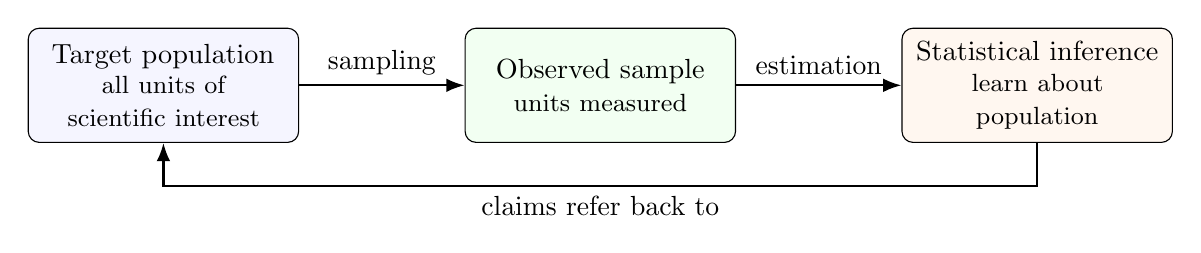
\begin{tikzpicture}[
  >=Latex,
  box/.style={
    draw,
    rounded corners,
    align=center,
    minimum height=1.45cm,
    text width=3.2cm
  },
  arrow/.style={->, thick}
]

  \node[box, fill=blue!4] (pop)
    {Target population\\\small all units of\\\small scientific interest};

  \node[box, fill=green!5, right=2.1cm of pop] (sample)
    {Observed sample\\\small units measured};

  \node[box, fill=orange!6, right=2.1cm of sample] (inference)
    {Statistical inference\\\small learn about\\\small population};

  \draw[arrow] (pop) -- node[above]{sampling} (sample);
  \draw[arrow] (sample) -- node[above]{estimation} (inference);

  \draw[arrow]
    (inference.south) -- ++(0,-0.55)
    -- node[below]{claims refer back to}
    ($(pop.south)+(0,-0.55)$)
    -- (pop.south);

\end{tikzpicture}
\caption{A sample is a finite piece of evidence about a larger target population.}
\end{figure}

\subsection{Target Parameter and Estimand}

After specifying the population, the next task is to specify the number, function, or distributional feature we want to learn.

\begin{definition}[Target parameter]
A \emph{target parameter} is a well-defined summary of the target population distribution. It is the quantity the analysis aims to learn. The word \emph{estimand} is often used synonymously, especially when emphasizing the quantity to be estimated.
\end{definition}

Examples include:
\begin{itemize}
  \item the population mean systolic blood pressure, $\E(W)$;
  \item the population prevalence of HIV infection, $\Prob(Y=1)$;
  \item the difference in mean blood pressure between people observed to take statins and people observed not to take statins, $\E(Y\given A=1)-\E(Y\given A=0)$;
  \item a regression function such as $w \mapsto \E(Y\given W=w)$.
\end{itemize}

A parameter is not the same thing as an observed data point. If one patient has systolic blood pressure 135, that is a measurement. The population mean systolic blood pressure is a property of the distribution of blood pressure in the population. It would still be well-defined even before drawing a sample.

\begin{example}[A descriptive parameter]
Let $W$ denote age and $Y$ denote systolic blood pressure for members of a target population. The parameter $\E(Y)$ is the average systolic blood pressure in that population. The parameter $\E(Y\given W\ge 65)$ is the average systolic blood pressure among the subgroup of the population aged at least 65.
\end{example}

At this point in the course, most parameters are descriptive statistical parameters. Later, causal inference will introduce counterfactual parameters such as $\E\{\Ya{1}\}-\E\{\Ya{0}\}$, which describe populations under interventions. The same discipline applies: first define the population, then define the parameter.

\subsection{Data as a Sample from a Population}

Let $O$ denote the full observed data record for one unit. In a simple study we may observe
\[
O=(W,A,Y),
\]
where $W$ is a vector of baseline covariates, $A$ is an exposure or treatment, and $Y$ is an outcome. A sample of size $n$ is written
\[
O_1,\ldots,O_n.
\]
A common statistical model assumes that these observations are independent and identically distributed:
\[
O_1,\ldots,O_n \iid P,
\]
where $P$ is the population distribution.

\begin{definition}[Iid sample]
The observations $O_1,\ldots,O_n$ are \emph{independent and identically distributed}, written $O_i \iid P$, if each observation has the same population distribution $P$ and the value of one observation does not affect the distribution of another.
\end{definition}

The iid assumption is a mathematical idealization. It is reasonable for some sampling schemes and unreasonable for others. For example, measurements from unrelated patients sampled independently from a clinic may be close to iid. Measurements from repeated visits of the same patient are not iid unless the unit is redefined or the dependence is modeled.

The distribution $P$ determines the target parameter. For instance, if the parameter is the population mean of $Y$, then
\[
\psi(P)=\E_P(Y).
\]
The notation $\psi(P)$ reminds us that a parameter is a function of the population distribution. If the population distribution changed, the parameter would generally change.

\subsection{Point Estimates and Estimators}

Because the population distribution $P$ is unknown, the target parameter $\psi(P)$ is unknown. Statistical inference uses the sample to construct an estimate.

\begin{definition}[Estimator and point estimate]
An \emph{estimator} is a rule or algorithm that maps a data set to a numerical estimate of a target parameter. A \emph{point estimate} is the numerical value produced by the estimator in the observed data.
\end{definition}

For example, suppose the target parameter is the population mean $\psi=\E(Y)$. The sample mean estimator is
\[
\hat\psi_n=\frac{1}{n}\sum_{i=1}^n Y_i.
\]
The expression $\hat\psi_n$ is the estimator as a formula. After observing the actual $Y_1,\ldots,Y_n$, the resulting number is the point estimate.

\begin{estimationbox}
For the population mean $\psi=\E(Y)$:
\[
\text{estimand: } \psi=\E(Y), \qquad
\text{estimator: } \hat\psi_n=\frac{1}{n}\sum_{i=1}^n Y_i.
\]
The estimator is the recipe. The point estimate is the recipe's output on the observed data.
\end{estimationbox}

The distinction between estimand, estimator, and estimate is essential.
\begin{itemize}
  \item The estimand is the population quantity we want.
  \item The estimator is the method used to learn it from data.
  \item The estimate is the number obtained in this particular sample.
\end{itemize}

\subsection{Standard Errors}

If the study were repeated on a new random sample from the same population, the estimate would usually change. A standard error describes this repeated-sampling variability.

\begin{definition}[Standard error]
The \emph{standard error} of an estimator $\hat\psi_n$ is the standard deviation of its sampling distribution:
\[
\operatorname{SE}(\hat\psi_n)=\sqrt{\Var(\hat\psi_n)}.
\]
An \emph{estimated standard error} is a data-based estimate of this quantity.
\end{definition}

For the sample mean under iid sampling with $\Var(Y)=\sigma^2<\infty$,
\[
\Var(\hat\psi_n)
=\Var\left(\frac{1}{n}\sum_{i=1}^n Y_i\right)
=\frac{1}{n^2}\sum_{i=1}^n \Var(Y_i)
=\frac{n\sigma^2}{n^2}
=\frac{\sigma^2}{n}.
\]
Thus
\[
\operatorname{SE}(\hat\psi_n)=\frac{\sigma}{\sqrt n}.
\]
Since $\sigma$ is unknown, it is commonly replaced by the sample standard deviation $s_n$, yielding
\[
\widehat{\operatorname{SE}}(\hat\psi_n)=\frac{s_n}{\sqrt n}.
\]

The standard error is not the same as the standard deviation of $Y$. The standard deviation of $Y$ describes variability among individuals in the population. The standard error describes variability of the estimator across repeated samples.

\subsection{Confidence Intervals}

A point estimate gives one best guess. A confidence interval gives a range of values that accounts for sampling variability.

Many estimators used in large samples are approximately Normal:
\[
\hat\psi_n \approx \operatorname{Normal}\{\psi,\operatorname{SE}(\hat\psi_n)^2\}.
\]
When an estimator is approximately Normal and its standard error can be estimated, a common Wald-style $95\%$ confidence interval is
\[
\hat\psi_n \pm 1.96\,\widehat{\operatorname{SE}}(\hat\psi_n).
\]

\begin{definition}[Frequentist confidence interval]
A procedure for constructing $95\%$ confidence intervals has $95\%$ coverage if, under repeated sampling from the same population, approximately $95\%$ of the intervals it produces contain the true target parameter.
\end{definition}

The interpretation is about the procedure, not about the fixed realized interval. In frequentist inference the parameter $\psi$ is treated as fixed. The random object is the interval, because the interval changes from sample to sample.

\begin{figure}[H]
\centering
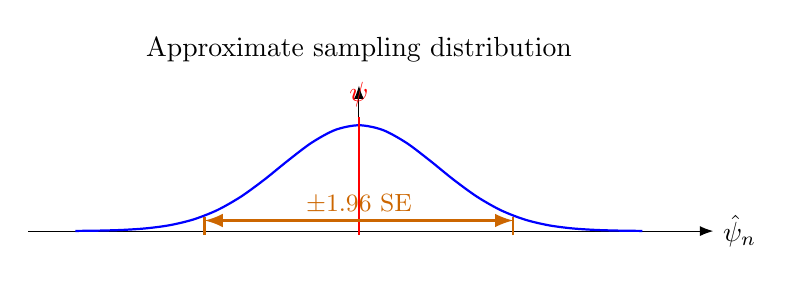
\begin{tikzpicture}[x=1.0cm,y=0.42cm,>=Latex]

  % axes
  \draw[->] (-4.2,0) -- (4.5,0) node[right] {$\hat\psi_n$};
  \draw[->] (0,0) -- (0,4.4);

  % normal curve
  \draw[
    domain=-3.6:3.6,
    smooth,
    variable=\x,
    blue,
    thick
  ]
  plot ({\x},{3.2*exp(-0.5*\x*\x)});

  % true parameter line
  \draw[red,thick]
    (0,-0.12) -- (0,3.45)
    node[above] {$\psi$};

  % CI markers
  \draw[orange!80!black,thick]
    (-1.96,-0.12) -- (-1.96,0.42);

  \draw[orange!80!black,thick]
    (1.96,-0.12) -- (1.96,0.42);

  % interval arrow
  \draw[<->,orange!80!black,thick]
    (-1.96,0.32)
    -- 
    (1.96,0.32);

  % interval label BELOW the line
  \node[
    orange!80!black,
    font=\small
  ]
  at (0,0.82)
  {$\pm 1.96\,\operatorname{SE}$};

  % top title with proper spacing
  \node[align=center]
    at (0,5.5)
    {Approximate sampling distribution};

\end{tikzpicture}

\caption{
A Wald interval uses the approximate Normal sampling distribution of the estimator.
}
\end{figure}

\subsection{Hypothesis Tests}

A hypothesis test turns data into a decision about a proposed value or claim.

\begin{definition}[Null and alternative hypotheses]
A \emph{null hypothesis} $H_0$ is a default claim about the target parameter, often representing no difference or no association. An \emph{alternative hypothesis} $H_1$ is the claim against which the null is compared.
\end{definition}

For example, if $\psi$ is a difference in population means, a common null hypothesis is
\[
H_0:\psi=0,
\]
with a two-sided alternative
\[
H_1:\psi\ne 0.
\]
If $\hat\psi_n$ is approximately Normal, a Wald test statistic is
\[
Z=\frac{\hat\psi_n-\psi_0}{\widehat{\operatorname{SE}}(\hat\psi_n)},
\]
where $\psi_0$ is the value specified by the null hypothesis. Under $H_0$ and appropriate regularity conditions, $Z$ is approximately standard Normal. Large values of $\abs{Z}$ are evidence against $H_0$.

The $p$-value for a two-sided Wald test is
\[
p=2\{1-\Phi(\abs{Z})\},
\]
where $\Phi$ is the standard Normal cumulative distribution function.

\begin{keyidea}
Point estimates, standard errors, confidence intervals, and hypothesis tests are all tools for learning about a target parameter. None of them is meaningful until the target population and target parameter have been clearly defined.
\end{keyidea}

\lecture{1.2}{Frequentist and Bayesian Perspectives}
\label{lec:1-2}

\subsection{Frequentist Interpretation of Probability}

In the frequentist view, probabilities describe long-run relative frequencies in a repeatable process or proportions in a target population. If $A$ is an indicator that a person received a monoclonal antibody infusion and $Y$ is an indicator of HIV infection, then
\[
\Prob(A=1,Y=1)
\]
can be read as the proportion of the target population for whom both $A=1$ and $Y=1$.

This interpretation also applies to conditional probabilities. The probability
\[
\Prob(Y=1\given A=1)
\]
is the proportion infected among the subgroup who received monoclonal antibodies. The conditioning event defines the subgroup; the probability describes the fraction of that subgroup with the outcome.

For continuous variables the exact phrase "proportion with $W=w$" may be inappropriate because $\Prob(W=w)$ can equal zero. In that setting probability is described by densities, distribution functions, and probabilities of intervals such as $\Prob(60\le W\le 70)$. The conceptual role is the same: probability describes how values are distributed in a population or under a random experiment.

\subsection{Bayesian Updating}

The Bayesian view treats unknown quantities as objects about which uncertainty can be expressed probabilistically. A Bayesian analysis begins with a prior distribution, combines it with the likelihood supplied by the data, and obtains a posterior distribution.

\begin{definition}[Bayesian update]
Let $\theta$ denote an unknown parameter and let $O_1,\ldots,O_n$ denote observed data. A Bayesian analysis specifies a prior density $\pi(\theta)$ and a likelihood $L(\theta;O_1,\ldots,O_n)$. The posterior density is
\[
\pi(\theta\given O_1,\ldots,O_n)
=
\frac{L(\theta;O_1,\ldots,O_n)\pi(\theta)}
{\int L(t;O_1,\ldots,O_n)\pi(t)\,dt}.
\]
\end{definition}

In words, the posterior distribution is the updated state of uncertainty after seeing the data. The denominator makes the posterior integrate to one. It also shows a central feature of Bayesian inference: prior beliefs and the likelihood both contribute to the final answer.

For example, if $\theta$ is the prevalence of a disease, a Bayesian credible interval might be interpreted as an interval containing $\theta$ with posterior probability $0.95$, conditional on the model and prior. This differs from a frequentist confidence interval, whose $95\%$ statement concerns repeated-sampling coverage of the interval construction procedure.

\subsection{Repeated-Sampling Properties}

Frequentist inference evaluates statistical procedures by imagining repeated samples from the same population. If the study were repeated many times, each repetition would produce a new data set, a new point estimate, a new confidence interval, and perhaps a new hypothesis test decision.

\begin{figure}[H]
\centering
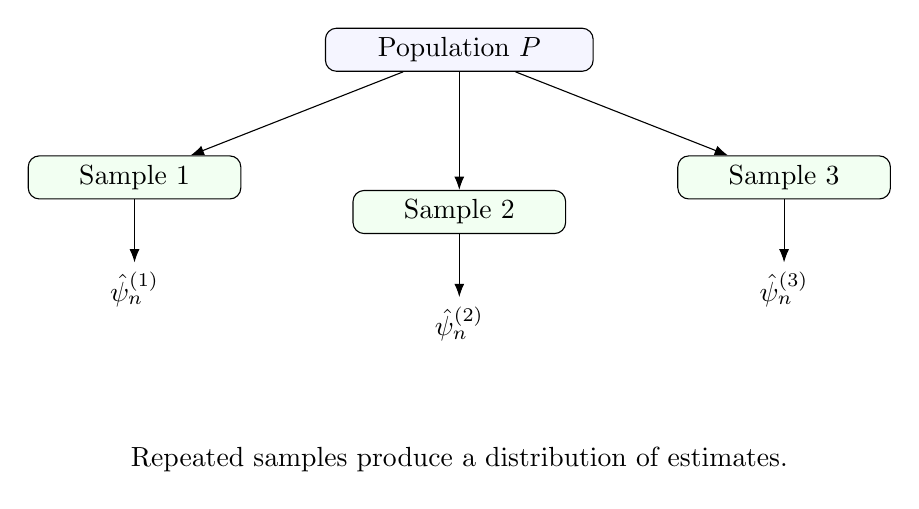
\begin{tikzpicture}[node distance=1.5cm,>=Latex]
  \node[draw, rounded corners, fill=blue!4, minimum width=3.4cm] (pop) {Population $P$};
  \node[draw, rounded corners, fill=green!5, below left=of pop, minimum width=2.7cm] (s1) {Sample 1};
  \node[draw, rounded corners, fill=green!5, below=of pop, minimum width=2.7cm] (s2) {Sample 2};
  \node[draw, rounded corners, fill=green!5, below right=of pop, minimum width=2.7cm] (s3) {Sample 3};
  \node[below=.8cm of s1] (e1) {$\hat\psi_n^{(1)}$};
  \node[below=.8cm of s2] (e2) {$\hat\psi_n^{(2)}$};
  \node[below=.8cm of s3] (e3) {$\hat\psi_n^{(3)}$};
  \draw[->] (pop) -- (s1);
  \draw[->] (pop) -- (s2);
  \draw[->] (pop) -- (s3);
  \draw[->] (s1) -- (e1);
  \draw[->] (s2) -- (e2);
  \draw[->] (s3) -- (e3);
  \node[align=center, below=1.1cm of e2] {Repeated samples produce a distribution of estimates.};
\end{tikzpicture}
\caption{Frequentist properties describe how a procedure behaves over repeated samples.}
\end{figure}

The phrase "good procedure" means that the procedure reliably achieves its stated goal over these repetitions. A good estimator is close to the truth on average or in large samples. A good confidence interval procedure contains the true parameter at its advertised rate. A good test rejects false null hypotheses often while controlling false rejection under the null.

\subsection{Bias}

\begin{definition}[Bias]
The finite-sample bias of an estimator $\hat\psi_n$ for a parameter $\psi$ is
\[
\Bias(\hat\psi_n)=\E(\hat\psi_n)-\psi,
\]
where the expectation is taken over repeated samples from the population.
\end{definition}

Bias is an average error across repeated experiments. It is not the error in one realized data set. An estimator can be biased and still sometimes be close to the truth; it can also be unbiased and still be highly variable.

\begin{example}[Bias of the sample mean]
If $Y_1,\ldots,Y_n \iid P$ and $\psi=\E(Y)$, then the sample mean is unbiased:
\[
\E(\hat\psi_n)
=\E\left(\frac{1}{n}\sum_{i=1}^nY_i\right)
=\frac{1}{n}\sum_{i=1}^n\E(Y_i)
=\frac{1}{n}\sum_{i=1}^n\psi
=\psi.
\]
Therefore $\Bias(\hat\psi_n)=0$.
\end{example}

Large-sample theory often focuses on whether the bias disappears as $n$ grows. An estimator is consistent if it converges in probability to the truth:
\[
\hat\psi_n \overset{P}{\longrightarrow} \psi.
\]
Consistency is stronger than saying the estimator is approximately unbiased in large samples, because it also requires the estimator's variability to vanish.

\subsection{Sampling Distribution}

\begin{definition}[Sampling distribution]
The \emph{sampling distribution} of an estimator is the probability distribution of the estimator over repeated samples from the same population.
\end{definition}

The sampling distribution answers the question: if we repeatedly collected samples of size $n$ and computed the same estimator each time, what values would the estimator take and how often?

For the sample mean, the central limit theorem gives an approximate answer. If $Y_1,\ldots,Y_n$ are iid with mean $\psi$ and variance $\sigma^2<\infty$, then
\[
\frac{\hat\psi_n-\psi}{\sigma/\sqrt n}
\overset{d}{\longrightarrow}
\operatorname{Normal}(0,1).
\]
Equivalently, for large $n$,
\[
\hat\psi_n \approx \operatorname{Normal}\left(\psi,\frac{\sigma^2}{n}\right).
\]
This approximation is the basis for many standard errors, confidence intervals, and Wald tests.

\subsection{Coverage Probability}

Suppose an interval procedure maps each data set to an interval $C_n$. For example,
\[
C_n=\left[
\hat\psi_n-1.96\,\widehat{\operatorname{SE}}(\hat\psi_n),
\hat\psi_n+1.96\,\widehat{\operatorname{SE}}(\hat\psi_n)
\right].
\]

\begin{definition}[Coverage probability]
The coverage probability of an interval procedure $C_n$ is
\[
\Prob\{\psi\in C_n\},
\]
where the probability is over repeated samples. A nominal $95\%$ confidence interval procedure aims to have coverage probability close to $0.95$.
\end{definition}

Coverage is a property of the procedure, not a property of the one interval obtained in the observed data. Once a particular interval has been computed, it either contains the fixed parameter or it does not. The frequentist probability statement refers to what would happen if the entire data-generating process were repeated.

\subsection{Power}

Hypothesis testing has its own repeated-sampling properties. Consider a test of
\[
H_0:\psi=\psi_0
\]
against some alternative. A test is a rule that rejects or fails to reject $H_0$.

\begin{definition}[Type I error and power]
The \emph{Type I error rate} is the probability of rejecting $H_0$ when $H_0$ is true. The \emph{power} of a test at a particular alternative value $\psi\ne\psi_0$ is the probability of rejecting $H_0$ when that alternative is true.
\end{definition}

Power depends on the true effect size, the sample size, the variability of the estimator, and the rejection threshold. Larger sample sizes often increase power because they reduce standard errors, making it easier to distinguish a real difference from sampling noise.

\begin{keyidea}
Frequentist and Bayesian analyses answer uncertainty questions differently. Frequentist statements evaluate procedures under repeated sampling. Bayesian statements update probability distributions for unknown quantities conditional on a prior, likelihood, and observed data.
\end{keyidea}

\lecture{1.3}{Probability Foundations}
\label{lec:1-3}

\subsection{Joint Distributions}

Probability distributions describe how variables vary in a population. When more than one variable is considered at the same time, the relevant object is a joint distribution.

\begin{definition}[Joint distribution]
For discrete variables $X$ and $Y$, the \emph{joint distribution} assigns probabilities
\[
\Prob(X=x,Y=y)
\]
to every possible pair of values $(x,y)$. For continuous variables, the joint distribution is described by a joint density or by probabilities of regions.
\end{definition}

The joint distribution contains information about each variable separately and about how the variables relate to each other. If $A$ denotes monoclonal antibody receipt and $Y$ denotes HIV infection status, then
\[
\Prob(A=1,Y=1)
\]
is the proportion of the target population who both received monoclonal antibodies and are HIV infected.

If $W$ denotes age, then
\[
\Prob(W=65,A=1,Y=0)
\]
is the proportion of the population who are exactly 65 years old, received monoclonal antibodies, and are not HIV infected. For continuous age, one would usually use an interval such as $\Prob(65\le W<66,A=1,Y=0)$.

\subsection{Marginal Distributions}

A marginal distribution describes one variable or a subset of variables without conditioning on the remaining variables.

\begin{definition}[Marginal distribution]
For discrete variables $X$ and $Y$, the marginal distribution of $X$ is obtained from the joint distribution by summing over all possible values of $Y$:
\[
\Prob(X=x)=\sum_y \Prob(X=x,Y=y).
\]
\end{definition}

This operation is called marginalization. It removes a variable by adding over its possible values.

\begin{example}[Marginalizing over treatment]
Let $Y$ be HIV infection status and $A$ be monoclonal antibody receipt. The population prevalence of HIV infection is
\[
\Prob(Y=1)
=\Prob(Y=1,A=0)+\Prob(Y=1,A=1)
=\sum_{a=0}^1 \Prob(Y=1,A=a).
\]
The total infected group is partitioned into infected nonrecipients and infected recipients.
\end{example}

\begin{figure}[H]
\centering
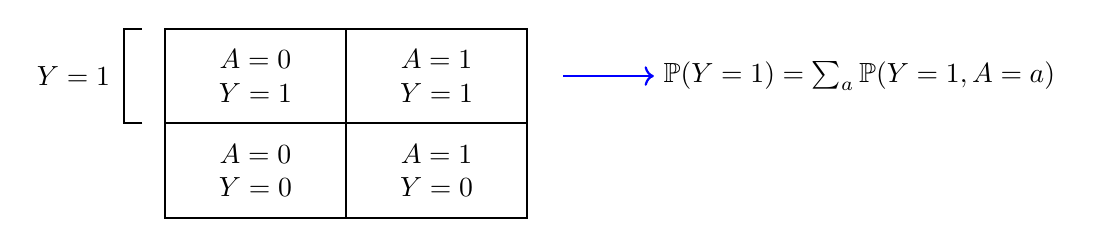
\begin{tikzpicture}[x=1.15cm,y=0.8cm]
  \draw[thick] (0,0) rectangle (4,3);
  \draw[thick] (2,0) -- (2,3);
  \draw[thick] (0,1.5) -- (4,1.5);
  \node at (1,2.25) {$A=0$\\$Y=1$};
  \node at (3,2.25) {$A=1$\\$Y=1$};
  \node at (1,.75) {$A=0$\\$Y=0$};
  \node at (3,.75) {$A=1$\\$Y=0$};
  \draw[thick] (-.25,1.5) -- (-.45,1.5) -- (-.45,3) -- (-.25,3);
  \node[left] at (-.5,2.25) {$Y=1$};
  \draw[->, thick, blue] (4.4,2.25) -- (5.4,2.25);
  \node[right] at (5.4,2.25) {$\Prob(Y=1)=\sum_a \Prob(Y=1,A=a)$};
\end{tikzpicture}
\caption{A marginal probability is obtained by adding joint probabilities over the variables being removed.}
\end{figure}

\subsection{Conditional Distributions}

Conditional probability describes a distribution inside a subgroup.

\begin{definition}[Conditional distribution]
For discrete variables $X$ and $Y$ with $\Prob(Y=y)>0$,
\[
\Prob(X=x\given Y=y)
=
\frac{\Prob(X=x,Y=y)}{\Prob(Y=y)}.
\]
\end{definition}

The denominator restricts attention to the subgroup with $Y=y$. The numerator counts the part of that subgroup that also has $X=x$. Thus conditional probability is a subgroup proportion.

\begin{example}[HIV infection among monoclonal recipients]
The probability of HIV infection among monoclonal antibody recipients is
\[
\Prob(Y=1\given A=1)
=
\frac{\Prob(Y=1,A=1)}{\Prob(A=1)}.
\]
This is not the fraction infected in the whole population. It is the fraction infected among the recipient subgroup.
\end{example}

With covariates, conditioning can define very specific subgroups. If $W=(W_1,W_2,W_3)$ represents age, BMI, and profession, then $W=w=(65,28.5,\text{nurse})$ defines the subgroup of 65-year-old nurses with BMI 28.5. A probability such as
\[
\Prob(Y=1\given A=1,W=w)
\]
is the probability of infection among monoclonal recipients in that covariate-defined subgroup.

\subsection{Chain Rule Factorization}

The definition of conditional probability can be rearranged to express a joint distribution as a product.

\begin{proposition}[Chain rule for two variables]
If $\Prob(X=x)>0$ and $\Prob(Y=y)>0$, then
\[
\Prob(X=x,Y=y)
=\Prob(X=x)\Prob(Y=y\given X=x)
=\Prob(Y=y)\Prob(X=x\given Y=y).
\]
\end{proposition}

\begin{proof}
By the definition of conditional probability,
\[
\Prob(Y=y\given X=x)
=\frac{\Prob(X=x,Y=y)}{\Prob(X=x)}.
\]
Multiplying both sides by $\Prob(X=x)$ gives
\[
\Prob(X=x)\Prob(Y=y\given X=x)=\Prob(X=x,Y=y).
\]
The second factorization follows by the same argument with $X$ and $Y$ interchanged.
\end{proof}

For three variables, repeated application gives
\[
\Prob(W=w,A=a,Y=y)
=
\Prob(W=w)\Prob(A=a\given W=w)\Prob(Y=y\given A=a,W=w).
\]
This factorization is a purely probabilistic identity. It does not by itself imply any causal ordering.

\subsection{Bayes Rule}

Bayes rule follows by combining the two chain rule factorizations.

\begin{proposition}[Bayes rule]
If $\Prob(Y=y)>0$, then
\[
\Prob(X=x\given Y=y)
=
\frac{\Prob(Y=y\given X=x)\Prob(X=x)}{\Prob(Y=y)}.
\]
Moreover,
\[
\Prob(Y=y)=\sum_x \Prob(Y=y\given X=x)\Prob(X=x)
\]
in the discrete case.
\end{proposition}

\begin{proof}
The chain rule gives
\[
\Prob(X=x,Y=y)=\Prob(Y=y\given X=x)\Prob(X=x).
\]
Substitute this expression into the definition
\[
\Prob(X=x\given Y=y)=\frac{\Prob(X=x,Y=y)}{\Prob(Y=y)}
\]
to obtain Bayes rule. The expression for $\Prob(Y=y)$ follows by marginalizing over $X$ and then applying the chain rule:
\[
\Prob(Y=y)
=\sum_x\Prob(X=x,Y=y)
=\sum_x\Prob(Y=y\given X=x)\Prob(X=x).
\]
\end{proof}

\subsection{From Joint to Marginal Probabilities}

The operation from joint to marginal probabilities is adding or integrating. For discrete variables,
\[
\Prob(X=x)=\sum_y \Prob(X=x,Y=y).
\]
For continuous variables with joint density $f_{X,Y}$,
\[
f_X(x)=\int f_{X,Y}(x,y)\,dy.
\]
The same principle applies to mixed or higher-dimensional data. For example,
\[
\Prob(W=25,A=1)
=
\sum_{y=0}^1 \Prob(W=25,A=1,Y=y),
\]
and
\[
\Prob(W=25)
=
\sum_{a=0}^1\sum_{y=0}^1 \Prob(W=25,A=a,Y=y).
\]

The idea is simple: to ignore a variable, add over every way that variable could have occurred.

\subsection{Conditional Probability as Subgroup Proportion}

The most important intuition in this lecture is that conditioning defines a subgroup.

\begin{keyidea}
Conditional probability equals a proportion within a subgroup:
\[
\Prob(\text{characteristic}\given \text{subgroup})
=
\frac{\Prob(\text{characteristic and subgroup})}
{\Prob(\text{subgroup})}.
\]
\end{keyidea}

For instance,
\[
\Prob(Y=1\given W=25,A=1)
=
\frac{\Prob(Y=1,W=25,A=1)}{\Prob(W=25,A=1)}.
\]
The denominator is the proportion of the whole population who are 25-year-old monoclonal recipients. The numerator is the proportion of the whole population who are 25-year-old monoclonal recipients and HIV infected. Dividing converts the whole-population proportion into a within-subgroup proportion.

This subgroup interpretation will be used constantly in causal inference. When we later write expressions such as $\E(Y\given A=1,W=w)$ or $\Prob(A=1\given W=w)$, the conditioning variables define the subgroup in which an outcome mean or treatment probability is being described.

\lecture{1.4}{Independence and Conditional Independence}
\label{lec:1-4}

\subsection{Definition of Independence}

Independence formalizes the idea that learning one piece of information does not change what we know about another.

\begin{definition}[Independence]
Events $B$ and $C$ are independent if
\[
\Prob(B,C)=\Prob(B)\Prob(C).
\]
Equivalently, when $\Prob(C)>0$ and $\Prob(B)>0$,
\[
\Prob(B\given C)=\Prob(B)
\qquad\text{and}\qquad
\Prob(C\given B)=\Prob(C).
\]
For random variables $X$ and $Y$, we write $X\ci Y$ if all events determined by $X$ are independent of all events determined by $Y$.
\end{definition}

The equivalence follows directly from conditional probability. If $\Prob(B,C)=\Prob(B)\Prob(C)$, then
\[
\Prob(B\given C)=\frac{\Prob(B,C)}{\Prob(C)}
=\frac{\Prob(B)\Prob(C)}{\Prob(C)}
=\Prob(B).
\]
Thus conditioning on $C$ does not change the probability of $B$.

\begin{keyidea}
Independence means that one variable carries no information about the other in the population.
\end{keyidea}

\subsection{Definition of Conditional Independence}

Conditional independence is independence within strata of another variable.

\begin{definition}[Conditional independence]
Events $B$ and $C$ are conditionally independent given $D$ if
\[
\Prob(B,C\given D)=\Prob(B\given D)\Prob(C\given D)
\]
whenever the conditioning probabilities are well-defined. Equivalently,
\[
\Prob(B\given C,D)=\Prob(B\given D).
\]
For random variables, we write $X\ci Y\given Z$.
\end{definition}

Plainly, $X\ci Y\given Z$ means that after restricting to people with the same value of $Z$, knowing $Y$ gives no additional information about $X$.

Conditional independence is not the same as marginal independence. It is possible for two variables to be associated in the full population but independent within strata of a third variable. It is also possible for two variables to be independent in the full population but associated after conditioning.

\subsection{Independence in Randomized Trials}

Consider a randomized trial in which $A$ indicates assignment to a vaccine arm, with
\[
\Prob(A=1)=\frac{1}{2}
\]
for every participant. Let $W$ denote age. Because the treatment assignment is generated by a random device that ignores age,
\[
\Prob(A=1\given W=w)=\Prob(A=1)=\frac{1}{2}
\]
for every age $w$ in the trial population. Hence $A\ci W$.

\begin{assumptionbox}
In an individually randomized trial with equal allocation, treatment assignment is independent of baseline covariates:
\[
A\ci W.
\]
In plain language, baseline characteristics do not help predict treatment assignment because the randomization mechanism did not use them.
\end{assumptionbox}

This independence is a design property. It is not discovered by observing that the treatment groups look similar in one finite sample. In a small randomized trial the realized treatment group may contain older participants by chance, but the assignment mechanism is still independent of age.

\subsection{Stratified Randomization}

Now suppose the trial uses stratified randomization by age. Participants younger than 65 receive vaccine with probability $1/2$, while participants aged at least 65 receive vaccine with probability $2/3$:
\[
\Prob(A=1\given W<65)=\frac{1}{2},
\qquad
\Prob(A=1\given W\ge 65)=\frac{2}{3}.
\]
In this design, $A$ and $W$ are not marginally independent. Knowing that someone is at least 65 changes the probability of treatment assignment.

However, within age strata, the assignment may still be randomized with respect to other baseline covariates. Let $Z$ denote congestive heart failure status. If the randomization rule uses age but not $Z$, then
\[
A\ci Z\given W.
\]
Among people of the same age stratum, knowing congestive heart failure status gives no additional information about treatment assignment.

\begin{figure}[H]
\centering
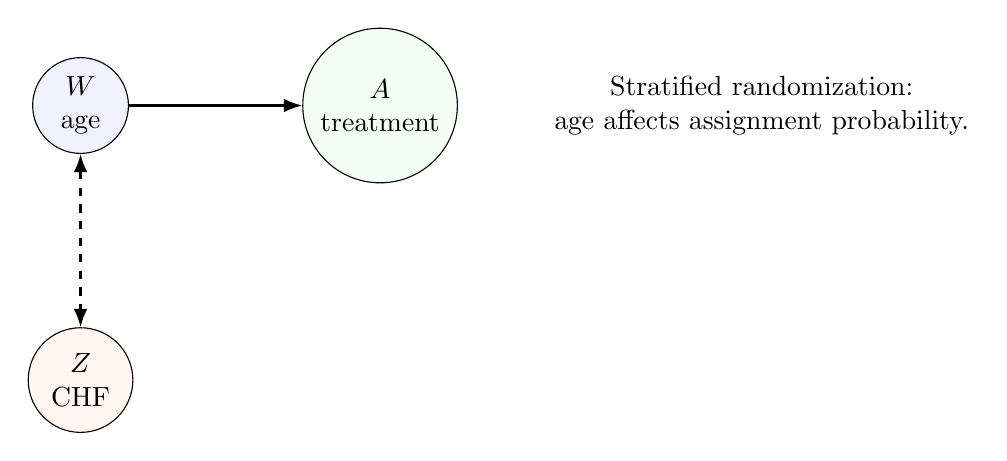
\begin{tikzpicture}[node distance=2.2cm,>=Latex]
  \node[draw, circle, fill=blue!5] (W) {$W$\\age};
  \node[draw, circle, fill=green!5, right=of W] (A) {$A$\\treatment};
  \node[draw, circle, fill=orange!6, below=of W] (Z) {$Z$\\CHF};
  \draw[->, thick] (W) -- (A);
  \draw[<->, thick, dashed] (W) -- (Z);
  \node[align=center, right=1.1cm of A] {Stratified randomization:\\age affects assignment probability.};
\end{tikzpicture}
\caption{In a stratified trial, treatment assignment can depend on the stratifying variable while remaining independent of other covariates within strata.}
\end{figure}

\subsection{Why Conditioning Can Remove Information}

Conditioning can remove information because it compares units only within a fixed subgroup. In the stratified randomization example, congestive heart failure status may be associated with age. In the full population, learning $Z$ tells us something about likely age, and age tells us something about treatment probability. Therefore $Z$ can be informative about $A$ marginally.

Once we condition on age, that indirect information path is removed. Among participants in the same age stratum, $Z$ no longer conveys information about the randomization probability. This is why
\[
A\nci Z
\qquad\text{but}\qquad
A\ci Z\given W
\]
can both be true.

The following table gives a concrete illustration:
\[
\begin{array}{c|cc}
& \Prob(A=1\given W,Z=0) & \Prob(A=1\given W,Z=1)\\
\hline
W<65 & 1/2 & 1/2\\
W\ge 65 & 2/3 & 2/3
\end{array}
\]
Within each age stratum, the treatment probability does not depend on $Z$. If people with $Z=1$ are more often in the older stratum, then $\Prob(A=1\given Z=1)$ can still exceed $\Prob(A=1\given Z=0)$ marginally.

\subsection{Why Conditional Independence Matters for Causal Inference}

Causal inference often requires comparing treated and untreated people who are similar with respect to variables that affect treatment and outcome. The mathematical language for this idea is conditional independence.

In later chapters, a central causal assumption for a binary treatment will take the form
\[
\Ya{a}\ci A\given W,
\qquad a\in\{0,1\}.
\]
This says that, among people with the same covariates $W$, treatment assignment $A$ carries no additional information about the counterfactual outcome under treatment level $a$. This is a causal version of "as-if randomized within strata of $W$."

The probability concepts in this lecture are therefore not merely technical preliminaries. They are the language used to state whether observed data can support causal comparisons.

\begin{keyidea}
Marginal independence asks whether two variables are unrelated in the whole population. Conditional independence asks whether they are unrelated after comparing only units in the same stratum of the conditioning variables.
\end{keyidea}

\lecture{1.5}{Expectation and Conditional Expectation}
\label{lec:1-5}

\subsection{Expected Value}

The expected value is the population average of a random variable.

\begin{definition}[Expected value]
For a discrete random variable $W$, the expected value, expectation, or mean is
\[
\E(W)=\sum_w w\,\Prob(W=w),
\]
where the sum is over all possible values of $W$. For a continuous random variable with density $f_W$, the expected value is
\[
\E(W)=\int w f_W(w)\,dw,
\]
provided the integral is well-defined.
\end{definition}

The discrete formula says: multiply each possible value by the proportion of the population with that value, then add across values. If $W$ is age, $\E(W)$ is the average age in the target population. If $W$ is systolic blood pressure, $\E(W)$ is the population mean systolic blood pressure.

\subsection{Expectation of Transformations}

Expectations can also be taken after transforming variables.

\begin{definition}[Expectation of a transformation]
For a function $f$, the expectation of $f(W)$ is
\[
\E\{f(W)\}=\sum_w f(w)\Prob(W=w)
\]
in the discrete case, or
\[
\E\{f(W)\}=\int f(w)f_W(w)\,dw
\]
in the continuous case.
\end{definition}

Examples include:
\[
\E(W^2), \qquad \E\{\log(W)\}, \qquad \E\{\ind(W\ge 65)\}.
\]
The last example is especially important because indicator functions convert events into numerical variables.

\subsection{Binary Variables and Probabilities}

If $Y$ is binary, with possible values 0 and 1, then its expectation equals the probability that it is 1:
\[
\E(Y)
=\sum_{y=0}^1 y\Prob(Y=y)
=0\cdot \Prob(Y=0)+1\cdot \Prob(Y=1)
=\Prob(Y=1).
\]
More generally, for any event $B$,
\[
\E\{\ind(B)\}=\Prob(B).
\]

\begin{keyidea}
Means and probabilities are not separate ideas for binary variables. The mean of a 0/1 variable is the proportion of the population with value 1.
\end{keyidea}

This fact is used constantly. If $Y$ is a disease indicator, then $\E(Y)$ is disease prevalence. If $A$ is a treatment indicator, then $\E(A)$ is the proportion treated.

\subsection{Conditional Expectation as Subgroup Mean}

Conditional expectation is the mean within a subgroup.

\begin{definition}[Conditional expectation for a discrete conditioning event]
For a discrete variable $W$ and an event $A=a$ with $\Prob(A=a)>0$,
\[
\E(W\given A=a)=\sum_w w\,\Prob(W=w\given A=a).
\]
\end{definition}

For example, if $W$ is age and $A=1$ indicates monoclonal antibody receipt, then
\[
\E(W\given A=1)
\]
is the average age among monoclonal antibody recipients. It is not the average age in the whole population.

If $Y$ is binary, then
\[
\E(Y\given A=1)=\Prob(Y=1\given A=1).
\]
Thus the conditional mean of a binary outcome is a conditional probability.

\subsection{Conditional Mean as a Function}

A conditional mean can be viewed as a function of the conditioning variables. The notation
\[
\E(W\given A)
\]
does not represent a single number until $A$ is fixed. It is a random variable whose value depends on the subgroup to which the unit belongs:
\[
\E(W\given A)
=
\begin{cases}
\E(W\given A=0), & A=0,\\
\E(W\given A=1), & A=1.
\end{cases}
\]

In contrast, $\E(W\given A=a)$ is a number once $a$ is specified.

\begin{figure}[H]
\centering
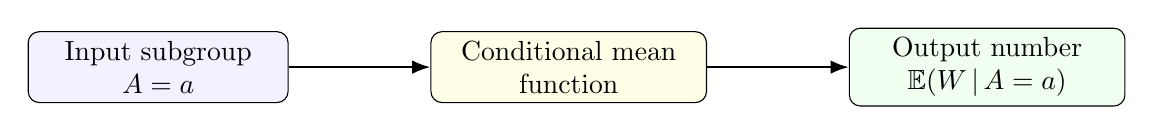
\begin{tikzpicture}[node distance=1.8cm,>=Latex]
  \node[draw, rounded corners, fill=blue!5, minimum width=3.3cm] (input) {Input subgroup\\$A=a$};
  \node[draw, rounded corners, fill=yellow!10, right=of input, minimum width=3.5cm] (machine) {Conditional mean\\function};
  \node[draw, rounded corners, fill=green!6, right=of machine, minimum width=3.5cm] (output) {Output number\\$\E(W\given A=a)$};
  \draw[->, thick] (input) -- (machine);
  \draw[->, thick] (machine) -- (output);
\end{tikzpicture}
\caption{A conditional expectation can be understood as a function that maps subgroup labels to subgroup means.}
\end{figure}

\subsection{Interpreting $\E(Y\given A,W)$}

The expression $\E(Y\given A,W)$ is a conditional mean function of both treatment and covariates. If $A$ is binary and $W$ is age, then
\[
(a,w)\mapsto \E(Y\given A=a,W=w)
\]
maps each treatment-age subgroup to the mean outcome in that subgroup.

If $Y$ is binary, then
\[
\E(Y\given A=a,W=w)=\Prob(Y=1\given A=a,W=w).
\]
For instance,
\[
\E(Y\given A=1,W=65)
\]
is the outcome prevalence among treated 65-year-olds. It should not be interpreted as the outcome that would occur if a particular person were treated. It is a descriptive mean among people actually observed with $A=1$ and $W=65$.

\begin{remark}
The expression $\E(Y\given A,W)$ is often estimated by regression. A fitted regression model is therefore best understood as an estimated conditional mean function. This interpretation is more fundamental for this course than interpreting individual regression coefficients.
\end{remark}

\lecture{1.6}{The Tower Rule}
\label{lec:1-6}

\subsection{Plain-Language Statement of the Tower Rule}

The tower rule is one of the most useful identities in probability and statistics. It says that an overall mean can be recovered by averaging subgroup means, using the subgroup sizes as weights.

\begin{keyidea}
The marginal mean equals the average of conditional means, weighted by subgroup prevalence.
\end{keyidea}

Suppose $W$ is systolic blood pressure and $A$ is sex at birth, coded as $A=0$ for one group and $A=1$ for another. Every person belongs to exactly one subgroup defined by $A$. If we know the mean blood pressure in each subgroup and the fraction of the population in each subgroup, then we can reconstruct the overall population mean.

In words:
\[
\text{overall mean}
=
\sum_{\text{subgroups}}
(\text{mean within subgroup})(\text{fraction in subgroup}).
\]

\subsection{Weighted Averages of Subgroup Means}

For a discrete grouping variable $A$, the tower rule is
\[
\E(W)=\sum_a \E(W\given A=a)\Prob(A=a).
\]
The weights $\Prob(A=a)$ must add to one. The quantities $\E(W\given A=a)$ are subgroup-specific means. The formula is therefore a weighted average of subgroup means.

\begin{figure}[H]
\centering
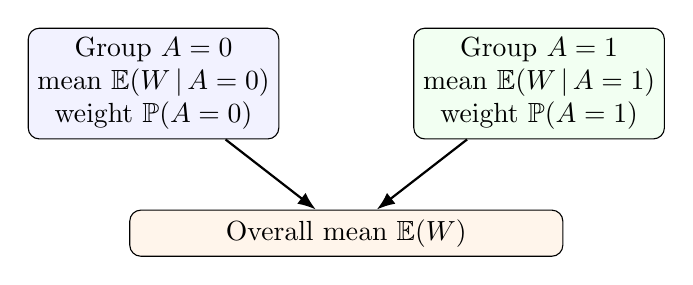
\begin{tikzpicture}[node distance=1.7cm,>=Latex]
  \node[draw, rounded corners, fill=blue!5, minimum width=3.0cm] (g0) {Group $A=0$\\mean $\E(W\given A=0)$\\weight $\Prob(A=0)$};
  \node[draw, rounded corners, fill=green!5, right=of g0, minimum width=3.0cm] (g1) {Group $A=1$\\mean $\E(W\given A=1)$\\weight $\Prob(A=1)$};
  \node[draw, rounded corners, fill=orange!8, below=1.6cm of $(g0)!0.5!(g1)$, minimum width=5.5cm] (overall) {Overall mean $\E(W)$};
  \draw[->, thick] (g0) -- (overall);
  \draw[->, thick] (g1) -- (overall);
\end{tikzpicture}
\caption{The tower rule combines subgroup means according to subgroup prevalence.}
\end{figure}

The rule is not an approximation. It is an identity, provided the expectations exist.

\subsection{Numeric Example}

Suppose the population is split into two groups:
\[
\Prob(A=0)=0.6,\qquad \Prob(A=1)=0.4.
\]
Suppose the subgroup means of systolic blood pressure are
\[
\E(W\given A=0)=120,
\qquad
\E(W\given A=1)=130.
\]
Then
\[
\E(W)
=\E(W\given A=0)\Prob(A=0)
+\E(W\given A=1)\Prob(A=1).
\]
Substituting the numbers,
\[
\E(W)
=120(0.6)+130(0.4)
=72+52
=124.
\]
The overall mean is 124. The group representing $60\%$ of the population contributes $60\%$ of its mean, and the group representing $40\%$ contributes $40\%$ of its mean.

\subsection{Probability Notation}

The same idea can be written compactly. For discrete $A$,
\[
\E(W)=\sum_a \E(W\given A=a)\Prob(A=a).
\]
For continuous $A$, the sum is replaced by an integral:
\[
\E(W)=\int \E(W\given A=a) f_A(a)\,da,
\]
where $f_A$ is the density of $A$.

When $A$ has three values, say $0,1,2$, the formula is
\[
\E(W)
=
\E(W\given A=0)\Prob(A=0)
+\E(W\given A=1)\Prob(A=1)
+\E(W\given A=2)\Prob(A=2).
\]

\subsection{Shorthand Form: $\E(W)=\E\{\E(W\given A)\}$}

The tower rule is often written as
\[
\E(W)=\E\{\E(W\given A)\}.
\]
This notation has two layers:
\begin{itemize}
  \item The inner expression $\E(W\given A)$ is a function of $A$. It assigns each subgroup its subgroup mean.
  \item The outer expectation averages that function over the population distribution of $A$.
\end{itemize}

For binary $A$,
\[
\E(W\given A)
=
\begin{cases}
\E(W\given A=0), & A=0,\\
\E(W\given A=1), & A=1.
\end{cases}
\]
Therefore
\[
\E\{\E(W\given A)\}
=
\E(W\given A=0)\Prob(A=0)
+\E(W\given A=1)\Prob(A=1).
\]

\subsection{Common Mistakes}

A common mistake is to confuse $\E(W\given A)$ with $\E(W)$. The conditional mean $\E(W\given A)$ is generally a random variable because it depends on $A$. The marginal mean $\E(W)$ is a single number.

Another common mistake is to omit the subgroup weights. If the subgroup means are 120 and 130, the overall mean is not necessarily $(120+130)/2$. That unweighted average is correct only if the two subgroups are equally prevalent. The correct weights are the population proportions $\Prob(A=a)$.

\begin{remark}
Conditioning creates subgroup-specific quantities. To return to a marginal quantity, we must average over the distribution of the conditioning variable.
\end{remark}

\subsection{Proof of the Tower Rule}

\begin{theorem}[Tower rule for a discrete grouping variable]
Let $W$ be a discrete random variable with finite expectation and let $A$ be a discrete random variable. Then
\[
\E(W)=\sum_a \E(W\given A=a)\Prob(A=a)
=\E\{\E(W\given A)\}.
\]
\end{theorem}

\begin{proof}
Start from the definition of expectation:
\[
\E(W)=\sum_w w\Prob(W=w).
\]
Marginalize over $A$:
\[
\Prob(W=w)=\sum_a \Prob(W=w,A=a).
\]
Substitute this into the expectation:
\[
\E(W)
=\sum_w w\sum_a \Prob(W=w,A=a).
\]
Switch the order of summation:
\[
\E(W)
=\sum_a\sum_w w\Prob(W=w,A=a).
\]
Use the chain rule $\Prob(W=w,A=a)=\Prob(W=w\given A=a)\Prob(A=a)$:
\[
\E(W)
=\sum_a\sum_w w\Prob(W=w\given A=a)\Prob(A=a).
\]
Because $\Prob(A=a)$ does not depend on $w$, move it outside the inner sum:
\[
\E(W)
=\sum_a \Prob(A=a)\sum_w w\Prob(W=w\given A=a).
\]
The inner sum is the conditional expectation $\E(W\given A=a)$, so
\[
\E(W)=\sum_a \E(W\given A=a)\Prob(A=a).
\]
The final expression is exactly $\E\{\E(W\given A)\}$.
\end{proof}

\subsection{Practice Problems}

\begin{exercise}[Three groups]
Let $A\in\{0,1,2\}$ with
\[
\Prob(A=0)=0.2,\qquad
\Prob(A=1)=0.5,\qquad
\Prob(A=2)=0.3.
\]
Suppose
\[
\E(W\given A=0)=9,\qquad
\E(W\given A=1)=10,\qquad
\E(W\given A=2)=14.
\]
Compute $\E(W)$.
\end{exercise}

\begin{proof}[Solution]
Apply the tower rule:
\[
\E(W)
=9(0.2)+10(0.5)+14(0.3)
=1.8+5+4.2
=11.
\]
\end{proof}

\begin{exercise}[Conditioning on two variables]
Let $A$ and $Z$ be discrete. Express $\E(W)$ using subgroup means defined by both $A$ and $Z$.
\end{exercise}

\begin{proof}[Solution]
The joint groups are defined by pairs $(a,z)$. The tower rule gives
\[
\E(W)
=
\sum_a\sum_z \E(W\given A=a,Z=z)\Prob(A=a,Z=z).
\]
Equivalently,
\[
\E(W)=\E\{\E(W\given A,Z)\}.
\]
\end{proof}

\begin{exercise}[A conditional version]
Let $A$ and $Z$ be discrete. Express $\E(W\given A=1)$ using subgroup means defined by $Z$ among those with $A=1$.
\end{exercise}

\begin{proof}[Solution]
Within the subgroup $A=1$, average over the distribution of $Z$ in that subgroup:
\[
\E(W\given A=1)
=
\sum_z \E(W\given A=1,Z=z)\Prob(Z=z\given A=1).
\]
This is the tower rule applied inside the $A=1$ subpopulation.
\end{proof}

\lecture{1.7}{Regression as Conditional Expectation Estimation}
\label{lec:1-7}

\subsection{Regression as Estimation of $\E(Y\given A,W)$}

In this course, regression will be used primarily as a tool for estimating conditional expectations. This is broader than the common habit of treating regression coefficients as the main scientific output.

\begin{definition}[Regression function]
For outcome $Y$, treatment or exposure $A$, and covariates $W$, the regression function is the conditional mean
\[
\Qbar(a,w)=\E(Y\given A=a,W=w).
\]
An estimator of this function will be denoted $\hat Q_n(a,w)$ or $\Qbar_n(a,w)$.
\end{definition}

The regression function is a machine: input a subgroup specification $(a,w)$, output the mean of $Y$ among units in that subgroup.

\begin{estimationbox}
Regression workflow for estimating $\E(Y\given A,W)$:
\begin{enumerate}
  \item Choose a regression method and a set of predictors involving $A$ and $W$.
  \item Fit the regression using the observed data $(Y_i,A_i,W_i)$.
  \item Obtain an estimated function $\Qbar_n(a,w)$.
  \item Evaluate $\Qbar_n(a,w)$ at covariate and treatment values of scientific interest.
\end{enumerate}
\end{estimationbox}

\subsection{Linear Regression}

A main-terms linear regression model for a scalar covariate $W$ is
\[
\E(Y\given A,W)=\beta_0+\beta_1A+\beta_2W.
\]
After fitting the model, the estimated regression function is
\[
\Qbar_n(a,w)=\hat\beta_0+\hat\beta_1a+\hat\beta_2w.
\]

For example, if the fitted coefficients are
\[
\hat\beta_0=3.27,\qquad
\hat\beta_1=0.17,\qquad
\hat\beta_2=-0.18,
\]
then
\[
\Qbar_n(a,w)=3.27+0.17a-0.18w.
\]
The estimated mean outcome for untreated people in age group 4 is
\[
\Qbar_n(0,4)=3.27+0.17(0)-0.18(4)=2.55.
\]
The estimated mean outcome for treated people in age group 7 is
\[
\Qbar_n(1,7)=3.27+0.17(1)-0.18(7)=2.18.
\]

The coefficient $\hat\beta_1$ is the modeled difference between treatment groups holding $W$ fixed by one unit of the model. Whether that coefficient is itself a meaningful scientific estimand depends on the question and on the model. The safer general view is that the fitted model estimates a conditional mean function.

\subsection{Logistic Regression}

When the outcome is binary, a conditional mean must lie between 0 and 1. Logistic regression ensures this by modeling the log-odds and then transforming back to a probability.

\begin{definition}[Expit function]
The expit function is
\[
\expit(x)=\frac{\exp(x)}{1+\exp(x)}
=\frac{1}{1+\exp(-x)}.
\]
It maps every real number to a value in $(0,1)$.
\end{definition}

A main-terms logistic regression model is
\[
\E(Y\given A,W)
=\Prob(Y=1\given A,W)
=\expit(\gamma_0+\gamma_1A+\gamma_2W).
\]
After fitting,
\[
\Qbar_n(a,w)=\expit(\hat\gamma_0+\hat\gamma_1a+\hat\gamma_2w).
\]

If logistic regression is used to estimate the treatment mechanism rather than the outcome regression, one might write
\[
g(w)=\Prob(A=1\given W=w)
=\expit(\alpha_0+\alpha_1w),
\]
with fitted estimator
\[
g_n(w)=\expit(\hat\alpha_0+\hat\alpha_1w).
\]
For example, if $\hat\alpha_0=-0.44$ and $\hat\alpha_1=0.07$, then
\[
g_n(2)=\expit(-0.44+0.07\cdot 2)\approx 0.43,
\]
and
\[
g_n(5)=\expit(-0.44+0.07\cdot 5)\approx 0.48.
\]

\subsection{Generalized Linear Models}

Linear and logistic regression are examples of generalized linear models (GLMs). A GLM specifies a conditional mean through a link function:
\[
h\{\E(Y\given X)\}=\eta(X),
\]
where $X$ denotes predictors, $h$ is the link function, and $\eta(X)$ is a linear predictor.

For linear regression, $h(u)=u$, so
\[
\E(Y\given X)=\eta(X).
\]
For logistic regression, $h(u)=\logit(u)$, so
\[
\logit\{\E(Y\given X)\}=\eta(X),
\qquad
\E(Y\given X)=\expit\{\eta(X)\}.
\]

In causal inference applications, GLMs are often used as nuisance regressions: intermediate models needed to estimate a target causal parameter. The final target is often not a regression coefficient.

\subsection{Main-Terms Models}

A main-terms model includes predictors additively on the scale of the linear predictor. With scalar $W$,
\[
\eta(A,W)=\beta_0+\beta_1A+\beta_2W.
\]
For several covariates $W=(W_1,\ldots,W_p)$,
\[
\eta(A,W)=\beta_0+\beta_1A+\beta_2W_1+\cdots+\beta_{p+1}W_p.
\]

Main-terms models borrow information across subgroups by imposing a simple structure. In the linear model above, the difference between $A=1$ and $A=0$ is the same at every value of $W$:
\[
\Qbar_n(1,w)-\Qbar_n(0,w)=\hat\beta_1.
\]
That restriction can be useful when data are limited, but it can be wrong if treatment-outcome associations vary across covariate values.

\subsection{Interaction Models}

Interaction models allow the relationship between one predictor and the outcome to depend on another predictor. A linear model with an $A$ by $W$ interaction is
\[
\E(Y\given A,W)=\beta_0+\beta_1A+\beta_2W+\beta_3AW.
\]
The fitted function is
\[
\Qbar_n(a,w)=\hat\beta_0+\hat\beta_1a+\hat\beta_2w+\hat\beta_3aw.
\]
Now the fitted difference between treatment groups at covariate value $w$ is
\[
\Qbar_n(1,w)-\Qbar_n(0,w)=\hat\beta_1+\hat\beta_3w.
\]
Thus the treatment contrast on the outcome scale is allowed to vary with $W$.

Polynomial terms are another way to add flexibility:
\[
\eta(A,W)=\beta_0+\beta_1A+\beta_2W+\beta_3W^2.
\]
The choice of regression formula determines what patterns can and cannot be represented by the fitted conditional mean.

\subsection{Using \texttt{glm} in R}

The R function \texttt{glm} fits generalized linear models. Suppose a data frame \texttt{covid19} contains:
\begin{itemize}
  \item \texttt{out}: an outcome variable $Y$;
  \item \texttt{treat}: a binary treatment variable $A$;
  \item \texttt{age\_grp}: an age group covariate $W$.
\end{itemize}

A main-terms linear regression for $\E(Y\given A,W)$ is fit by:
\begin{lstlisting}[language=R]
fit1 <- glm(out ~ treat + age_grp, data = covid19)
coef(fit1)
\end{lstlisting}

If the coefficient output is approximately
\begin{lstlisting}
(Intercept)      treat    age_grp
     3.2714     0.1692    -0.1780
\end{lstlisting}
then the fitted conditional mean is
\[
\Qbar_n(a,w)=3.2714+0.1692a-0.1780w.
\]

A main-terms logistic regression for the treatment probability $\Prob(A=1\given W)$ is fit by:
\begin{lstlisting}[language=R]
fit2 <- glm(treat ~ age_grp, data = covid19, family = binomial())
coef(fit2)
\end{lstlisting}

If the fitted coefficients are approximately $-0.4391$ for the intercept and $0.0729$ for \texttt{age\_grp}, then
\[
g_n(w)=\expit(-0.4391+0.0729w).
\]

\subsection{Prediction with \texttt{newdata}}

After fitting a regression, \texttt{predict} evaluates the fitted conditional mean at specified covariate values. For example:
\begin{lstlisting}[language=R]
aw_values <- data.frame(
  treat = c(0, 1),
  age_grp = c(4, 7)
)

predict(fit1, newdata = aw_values, type = "response")
\end{lstlisting}

The object \texttt{aw\_values} contains two subgroup specifications: $(A=0,W=4)$ and $(A=1,W=7)$. The call to \texttt{predict} returns the fitted means $\Qbar_n(0,4)$ and $\Qbar_n(1,7)$.

For logistic regression, \texttt{type = "response"} returns probabilities rather than log-odds:
\begin{lstlisting}[language=R]
w_values <- data.frame(age_grp = c(2, 5))
predict(fit2, newdata = w_values, type = "response")
\end{lstlisting}

These are estimates of $\Prob(A=1\given W=2)$ and $\Prob(A=1\given W=5)$ under the fitted logistic model.

\subsection{Regression Output as Subgroup Mean Estimates}

Regression output should be translated back into conditional mean estimates. Coefficients are ingredients for constructing the function $\Qbar_n$ or $g_n$.

\begin{keyidea}
A fitted regression is an estimated function. It takes subgroup-defining variables as input and returns an estimated subgroup mean or subgroup probability.
\end{keyidea}

Sometimes we need a function such as
\[
w\mapsto \E(Y\given A=1,W=w)
\]
rather than the full function $(a,w)\mapsto \E(Y\given A=a,W=w)$. There are two common approaches.

\paragraph{Pooling.}
Fit a regression using all observations and include $A$ and $W$ as predictors. If
\[
\Qbar_n(a,w)=\hat\beta_0+\hat\beta_1a+\hat\beta_2w,
\]
then estimate the treated conditional mean by setting $a=1$:
\[
\Qbar_{n,1}(w)=\Qbar_n(1,w)=\hat\beta_0+\hat\beta_1+\hat\beta_2w.
\]

\paragraph{Stratifying.}
Restrict the data to observations with $A=1$ and regress $Y$ on $W$ in that subset. A main-terms stratified fit might yield
\[
\Qbar_{n,1}(w)=\hat\eta_0+\hat\eta_1w.
\]

Pooling borrows information across treatment groups through the model structure. Stratifying avoids imposing a common structure across treatment groups but may use less data. Later causal estimators will use both ideas, often with more flexible regression methods.

\begin{remark}
Regression coefficients can be scientifically meaningful in special settings, but the general causal inference workflow is different: define the target estimand first, identify it in terms of observed-data quantities, and then use regression as needed to estimate those quantities.
\end{remark}


\chapterheading{2}{Asking Causal Questions}
\lecture{2.1}{From Association to Causation}
\label{lec:2-1}

\subsection{Motivating Example: Early Imaging for Back Pain}

Consider older adults who visit primary care for a new episode of back pain. A clinically natural question is whether early lumbar spinal imaging improves later outcomes. The exposure $A$ might indicate whether a patient received imaging within six weeks of the index visit. Outcomes $Y$ might include pain, disability, depression, anxiety, and later health care utilization, measured over months of follow-up.

This setting is useful because the causal question sounds simple, but the data-generating process is not simple. Physicians do not order early imaging at random. They may be more likely to order imaging for patients with severe pain, neurological symptoms, prior cancer, anxiety about serious disease, unusual examination findings, better insurance access, or preferences for aggressive diagnostic workups. Many of these same factors can also predict later disability and health care use.

\begin{figure}[H]
\centering
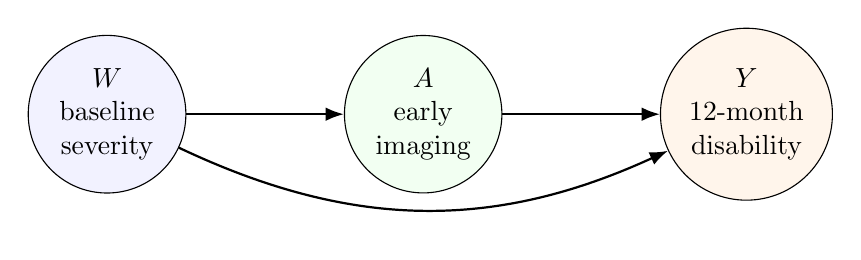
\begin{tikzpicture}[node distance=2.0cm,>=Latex]
  \node[draw, circle, fill=blue!5] (W) {$W$\\baseline\\severity};
  \node[draw, circle, fill=green!5, right=of W] (A) {$A$\\early\\imaging};
  \node[draw, circle, fill=orange!8, right=of A] (Y) {$Y$\\12-month\\disability};
  \draw[->, thick] (W) -- (A);
  \draw[->, thick] (W) to[bend right=25] (Y);
  \draw[->, thick] (A) -- (Y);
\end{tikzpicture}
\caption{A simplified causal story for early imaging. Baseline factors may affect both imaging and later disability.}
\end{figure}

The diagram is not a conclusion from the data. It is a scientific description of what might be happening. The arrow $W\to A$ says that baseline factors influence the probability of imaging. The arrow $W\to Y$ says that the same or related baseline factors influence disability. The arrow $A\to Y$ is the possible causal effect of imaging that motivates the study.

\subsection{Associative Analysis}

An associative analysis summarizes relationships in the observed population. For example, one might compare
\[
\E(Y\given A=1)
\quad\text{and}\quad
\E(Y\given A=0),
\]
the average disability score among patients who were observed to receive early imaging and the average disability score among patients who were observed not to receive early imaging.

\begin{definition}[Association]
An \emph{association} is a contrast between features of the observed data distribution, such as
\[
\E(Y\given A=1)-\E(Y\given A=0).
\]
It describes how outcomes differ between groups as they actually occurred.
\end{definition}

The observed mean difference
\[
\E(Y\given A=1)-\E(Y\given A=0)
\]
is meaningful as a descriptive parameter. It answers: among patients in the target population, how do observed outcomes differ between those who did and did not receive early imaging?

It does not by itself answer: what would happen if the imaging decision were changed? If patients receiving early imaging tend to have worse baseline symptoms, then the observed imaging group may have worse later disability even if imaging itself has no harmful effect.

\subsection{Causal Analysis}

Causal analysis asks questions about populations under interventions. Instead of comparing patients as they happened to be treated, we compare hypothetical worlds in which treatment assignment is deliberately changed.

\begin{definition}[Causal analysis]
A \emph{causal analysis} targets a feature of a population under one or more interventions. For a binary treatment $A$, a causal analysis might compare the mean outcome if everyone received $A=1$ with the mean outcome if everyone received $A=0$.
\end{definition}

For the back pain example, the causal question might be:
\begin{quote}
What would be the average 12-month disability score if all eligible older adults with a new primary care visit for back pain received early imaging, compared with if none received early imaging?
\end{quote}

This question is not merely about the subgroup who actually received imaging. It is about the same target population under two alternative interventions.

\begin{keyidea}
Associative analysis compares observed groups. Causal analysis compares intervention-generated worlds.
\end{keyidea}

\subsection{Population under Intervention}

To formalize the difference, imagine two intervention regimes:
\[
\doop(A=1): \text{ assign everyone to early imaging},
\]
and
\[
\doop(A=0): \text{ assign everyone to no early imaging}.
\]
The notation $\doop(A=a)$ emphasizes that the treatment value is set by intervention rather than merely observed.

Let $\E_{\doop(A=1)}(Y)$ denote the mean disability score in the population under the intervention assigning everyone to early imaging. Let $\E_{\doop(A=0)}(Y)$ denote the corresponding mean under no early imaging. A causal contrast is
\[
\E_{\doop(A=1)}(Y)-\E_{\doop(A=0)}(Y).
\]

\begin{figure}[H]
\centering
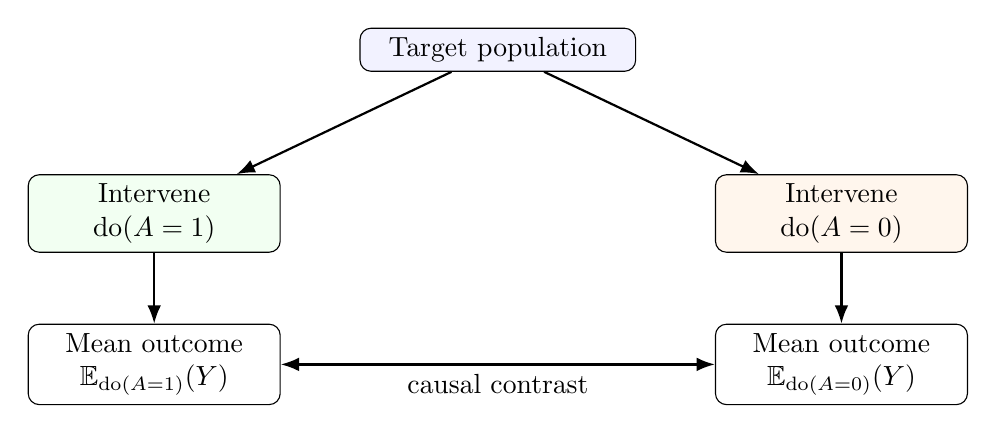
\begin{tikzpicture}[node distance=1.2cm,>=Latex]
  \node[draw, rounded corners, fill=blue!5, minimum width=3.5cm] (pop) {Target population};
  \node[draw, rounded corners, fill=green!5, below left=1.3cm and 1.0cm of pop, minimum width=3.2cm] (world1) {Intervene\\$\doop(A=1)$};
  \node[draw, rounded corners, fill=orange!7, below right=1.3cm and 1.0cm of pop, minimum width=3.2cm] (world0) {Intervene\\$\doop(A=0)$};
  \node[draw, rounded corners, below=.9cm of world1, minimum width=3.2cm] (y1) {Mean outcome\\$\E_{\doop(A=1)}(Y)$};
  \node[draw, rounded corners, below=.9cm of world0, minimum width=3.2cm] (y0) {Mean outcome\\$\E_{\doop(A=0)}(Y)$};
  \draw[->, thick] (pop) -- (world1);
  \draw[->, thick] (pop) -- (world0);
  \draw[->, thick] (world1) -- (y1);
  \draw[->, thick] (world0) -- (y0);
  \draw[<->, thick] (y1) -- node[below]{causal contrast} (y0);
\end{tikzpicture}
\caption{A causal contrast compares the same population under different interventions.}
\end{figure}

\subsection{Why Data Alone Cannot Answer Causal Questions}

The observed data contain outcomes under the treatment decisions that actually occurred. They do not automatically contain outcomes under alternative treatment policies. If a patient received imaging, we observe that patient's outcome after imaging. We do not also observe that same patient's outcome under no imaging at the same time and in the same circumstances.

This is the central reason causal inference requires assumptions. The data may show that early imaging patients had higher health care utilization. That observed association could reflect a causal effect of imaging, but it could also reflect that patients selected for imaging had more severe or concerning presentations.

Randomized trials help because the treatment assignment mechanism is controlled by design. Even then, the causal question may go beyond the literal trial data. Participants may not adhere to assigned treatment, clinicians may deviate from protocol, and follow-up may be incomplete. A question such as "what would happen if everyone complied and no one dropped out?" still refers to a hypothetical intervention.

\subsection{Untestable Assumptions}

\begin{assumptionbox}
Causal inference from observational data, and from many randomized trials with nonadherence or missingness, requires assumptions that cannot be verified from the observed data distribution alone. These assumptions connect observed outcomes to outcomes that would have been seen under interventions.
\end{assumptionbox}

Untestable does not mean arbitrary. Good causal assumptions come from design knowledge, biology, clinical expertise, institutional knowledge, measurement details, and transparent reasoning. The point is that the observed data distribution cannot, by itself, distinguish all causal explanations that generate the same associations.

For the early imaging example, investigators must reason about questions such as:
\begin{itemize}
  \item Which baseline factors influence a clinician's decision to order imaging?
  \item Which baseline factors also influence later disability or health care use?
  \item Were those factors measured well enough to compare like with like?
  \item Is "early imaging" a sufficiently precise intervention?
\end{itemize}

The rest of the course develops a formal language for asking these questions, stating the necessary assumptions, and determining when causal parameters can be learned from observed data.

\lecture{2.2}{The Roadmap for Causal Analysis}
\label{lec:2-2}

\subsection{Overview}

Causal analysis is easiest to learn as a sequence of distinct tasks. Mixing these tasks is a common source of confusion. For example, fitting a regression model before defining the causal question often leads to interpreting a convenient coefficient rather than estimating a meaningful causal parameter.

\begin{keyidea}
The causal roadmap separates scientific definition, causal identification, statistical estimation, and interpretation. Each step answers a different question.
\end{keyidea}

\begin{figure}[H]
\centering
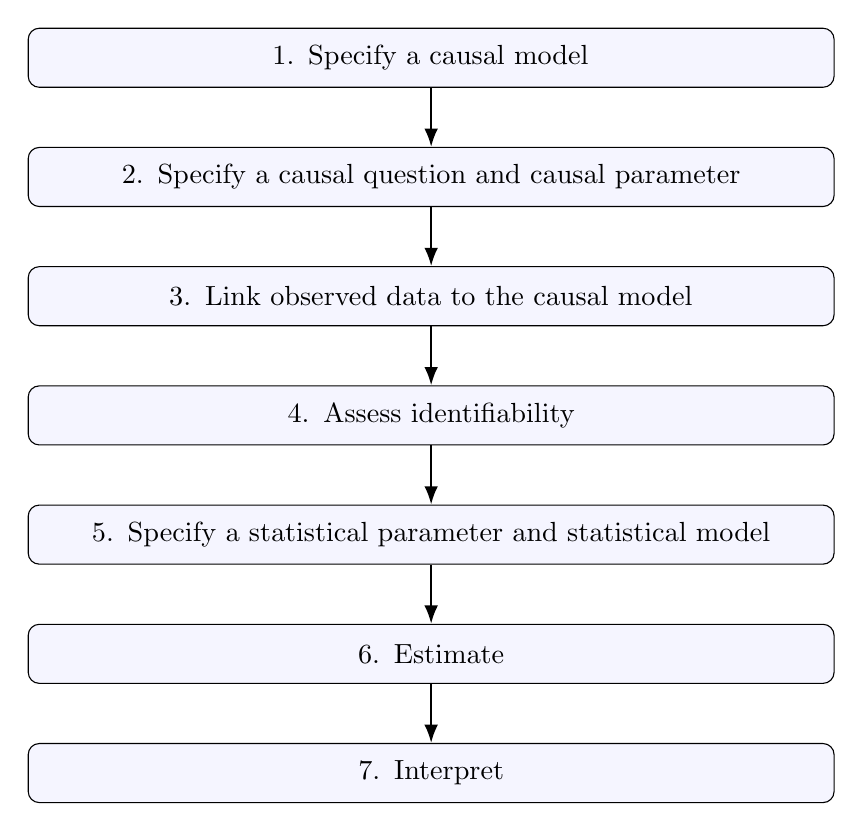
\begin{tikzpicture}[node distance=.75cm,>=Latex]
  \tikzset{box/.style={draw, rounded corners, fill=blue!4, text width=10cm, minimum height=.75cm}}
  \node[box] (s1) {1. Specify a causal model};
  \node[box, below=of s1] (s2) {2. Specify a causal question and causal parameter};
  \node[box, below=of s2] (s3) {3. Link observed data to the causal model};
  \node[box, below=of s3] (s4) {4. Assess identifiability};
  \node[box, below=of s4] (s5) {5. Specify a statistical parameter and statistical model};
  \node[box, below=of s5] (s6) {6. Estimate};
  \node[box, below=of s6] (s7) {7. Interpret};
  \foreach \a/\b in {s1/s2,s2/s3,s3/s4,s4/s5,s5/s6,s6/s7}
    \draw[->, thick] (\a) -- (\b);
\end{tikzpicture}
\caption{A practical roadmap for causal analysis.}
\end{figure}

\subsection{Specify a Causal Model}

A causal model represents scientific knowledge about how variables in the system relate to one another. At this stage we ask questions such as:
\begin{itemize}
  \item What factors affect whether a patient receives early imaging?
  \item What factors affect later disability?
  \item Which variables occur before treatment, during follow-up, or after the outcome?
  \item Which important causes were not measured?
\end{itemize}

In this course, causal models will often be represented by directed acyclic graphs (DAGs) and single world intervention graphs (SWIGs). The graph is not just a picture. It encodes assumptions about causes, noncauses, and conditional independencies.

\subsection{Specify a Causal Question and Parameter}

The causal question must state the intervention and the outcome. A vague question such as "Does imaging help?" is not yet a causal parameter. A more precise version is:
\begin{quote}
Among older adults with a new primary care visit for back pain, what is the difference in mean 12-month disability if everyone received lumbar imaging within six weeks versus if no one received lumbar imaging within six weeks?
\end{quote}

Using potential outcome notation, this question could be represented by
\[
\psi=\E\{\Yone\}-\E\{\Yzero\},
\]
where $\Yone$ is the outcome that would be observed under early imaging and $\Yzero$ is the outcome that would be observed under no early imaging.

\begin{definition}[Causal parameter]
A \emph{causal parameter} is a summary of the distribution of counterfactual variables in a target population. It is the causal estimand.
\end{definition}

\subsection{Link Observed Data to the Causal Model}

The causal model describes variables that may include both observed and unobserved quantities. The observed data describe what was actually measured. A common observed data structure for a point-treatment study is
\[
O=(W,A,Y),
\]
where $W$ denotes baseline covariates, $A$ observed treatment, and $Y$ observed outcome.

The analyst must state how these observed variables correspond to nodes in the causal model. If the graph contains an unmeasured severity variable $U$, the observed data do not include $U$. If the graph contains a broad baseline node $W$, the analyst must clarify which measured variables are included in $W$.

This step also includes assumptions that connect observed outcomes to counterfactual outcomes, especially consistency, introduced later in this chapter.

\subsection{Assess Identifiability}

Identification asks whether the causal parameter can be expressed as a function of the observed data distribution under the stated causal model.

\begin{definition}[Identifiability]
A causal parameter is \emph{identifiable} from the observed data distribution under a set of assumptions if all causal models satisfying those assumptions and producing the same observed data distribution imply the same value of the causal parameter.
\end{definition}

Plainly, identifiability asks: if we had infinite observed data from this study design, would the causal question be answerable? This question comes before estimation. No estimator, no matter how flexible, can recover a causal parameter that is not identified without additional assumptions.

\begin{identificationbox}
Identification is the bridge from counterfactual quantities to observed-data quantities. A typical goal is to replace a causal expression such as $\E\{\Ya{a}\}$ with an observed-data expression such as $\E\{\E(Y\given A=a,W)\}$ under appropriate assumptions.
\end{identificationbox}

\subsection{Specify Statistical Parameter and Model}

Once a causal parameter has been identified, the target becomes a statistical parameter of the observed data distribution. For example, an identification result might show that
\[
\E\{\Ya{a}\}=\E\{\E(Y\given A=a,W)\}.
\]
The right-hand side is an observed-data parameter. It depends on the distribution of $(W,A,Y)$, not directly on unobserved counterfactuals.

The statistical model describes what is assumed about the observed data distribution. A nonparametric model makes few restrictions. A parametric model might assume a specific logistic regression or linear regression form. The choice of statistical model affects estimation and inference, but it is conceptually separate from the causal identification assumptions.

\subsection{Estimate}

Estimation uses the finite sample to approximate the statistical parameter. If the identified parameter involves the conditional mean $\E(Y\given A=a,W)$, then an estimator may require fitting an outcome regression. If it involves $\Prob(A=a\given W)$, then an estimator may require fitting a propensity score.

\begin{estimationbox}
The estimation step answers a statistical question: given the identified observed-data parameter and a sample $O_1,\ldots,O_n$, how should we compute a numerical estimate and quantify uncertainty?
\end{estimationbox}

Estimation should not change the estimand. A regression coefficient may be easy to estimate, but it is not automatically the causal parameter. The target parameter should be defined before the estimator is chosen.

\subsection{Interpret}

The final step translates the estimate back into the scientific question while respecting the assumptions and limitations. Interpretation should state:
\begin{itemize}
  \item the target population;
  \item the intervention being compared;
  \item the outcome and time scale;
  \item the causal assumptions required;
  \item the statistical uncertainty;
  \item limitations from measurement, missing data, adherence, and generalizability.
\end{itemize}

A careful interpretation might say that the result estimates the mean difference in 12-month disability under two specified imaging policies, among patients represented by the study population, assuming the measured covariates were sufficient to control confounding, treatment was well-defined, and follow-up bias was adequately handled.

\lecture{2.3}{Causal Models and DAGs}
\label{lec:2-3}

\subsection{Why Graphical Models}

Causal questions require assumptions about how variables relate to one another. Graphical models provide a compact way to state those assumptions before analyzing the data.

Graphs are useful for three reasons. First, they force the analyst to name the variables believed to be relevant. Second, they make assumed causal relationships visible. Third, they translate scientific claims into mathematical restrictions that can be studied systematically.

\begin{keyidea}
A causal graph is a disciplined way to draw assumptions before drawing conclusions.
\end{keyidea}

For example, in a study of antihistamine use and asthma incidence among children, suppose:
\begin{itemize}
  \item $X_1$ is air pollution level;
  \item $X_2$ is biological sex;
  \item $X_3$ is bronchial reactivity;
  \item $A$ is antihistamine treatment;
  \item $Y$ is asthma incidence.
\end{itemize}
Subject-matter knowledge may suggest that pollution influences bronchial reactivity and antihistamine use, sex influences bronchial reactivity and asthma, and antihistamine use may influence asthma.

\subsection{Directed Acyclic Graphs}

\begin{definition}[Directed acyclic graph]
A \emph{directed acyclic graph} (DAG) is a graph consisting of nodes and directed edges, with no directed cycle. A directed cycle is a path following arrow directions that starts and ends at the same node.
\end{definition}

"Directed" means arrows have arrowheads. "Acyclic" means a variable cannot be its own cause through a sequence of arrows such as $A\to B\to C\to A$.

\begin{figure}[H]
\centering
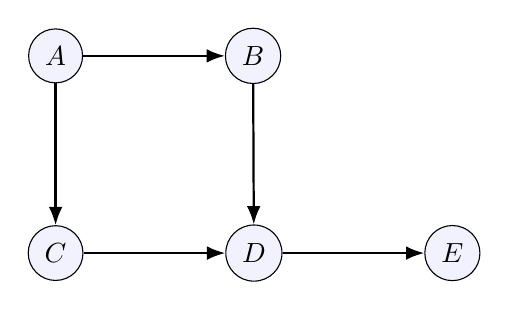
\begin{tikzpicture}[node distance=1.8cm,>=Latex]
  \node[draw, circle, fill=blue!5] (A) {$A$};
  \node[draw, circle, fill=blue!5, right=of A] (B) {$B$};
  \node[draw, circle, fill=blue!5, below=of A] (C) {$C$};
  \node[draw, circle, fill=blue!5, right=of C] (D) {$D$};
  \node[draw, circle, fill=blue!5, right=of D] (E) {$E$};
  \draw[->, thick] (A) -- (B);
  \draw[->, thick] (A) -- (C);
  \draw[->, thick] (B) -- (D);
  \draw[->, thick] (C) -- (D);
  \draw[->, thick] (D) -- (E);
\end{tikzpicture}
\caption{A directed acyclic graph with five nodes.}
\end{figure}

\subsection{Nodes and Edges}

\begin{definition}[Nodes and edges]
The \emph{nodes} or \emph{vertices} of a DAG represent variables. A \emph{directed edge} $X\to Y$ is an arrow from node $X$ to node $Y$. Two nodes are \emph{adjacent} if they are connected by an edge.
\end{definition}

A node can represent a scalar variable, such as treatment $A$, or a vector of variables, such as
\[
W=(W_1,\ldots,W_{30}),
\]
where $W$ is a baseline survey with 30 items. Whether variables should be collapsed into one node depends on the scientific question. If one survey item is the exposure of interest, it should not be hidden inside a broad $W$ node.

\subsection{Parents, Children, Ancestors, Descendants}

\begin{definition}[Family relationships in a DAG]
If $X\to Y$, then $X$ is a \emph{parent} of $Y$ and $Y$ is a \emph{child} of $X$. An \emph{ancestor} of $Y$ is any node with a directed path into $Y$. A \emph{descendant} of $X$ is any node reached by a directed path out of $X$.
\end{definition}

In the five-node graph above,
\[
\pa(D)=\{B,C\},
\qquad
\ch(A)=\{B,C\}.
\]
The ancestors of $E$ are $A,B,C,D$, and the descendants of $A$ are $B,C,D,E$.

\subsection{Causal Meaning of Arrows}

A causal DAG gives arrows a causal interpretation. An arrow $X\to Y$ means that $X$ is a direct cause of $Y$ relative to the variables included in the graph.

"Direct" is relative to the graph. If $X\to M\to Y$ and there is no arrow $X\to Y$, the graph says that $X$ may affect $Y$ through $M$ but has no direct effect on $Y$ not mediated by $M$, among the variables represented.

For the antihistamine example, one possible DAG is:

\begin{figure}[H]
\centering
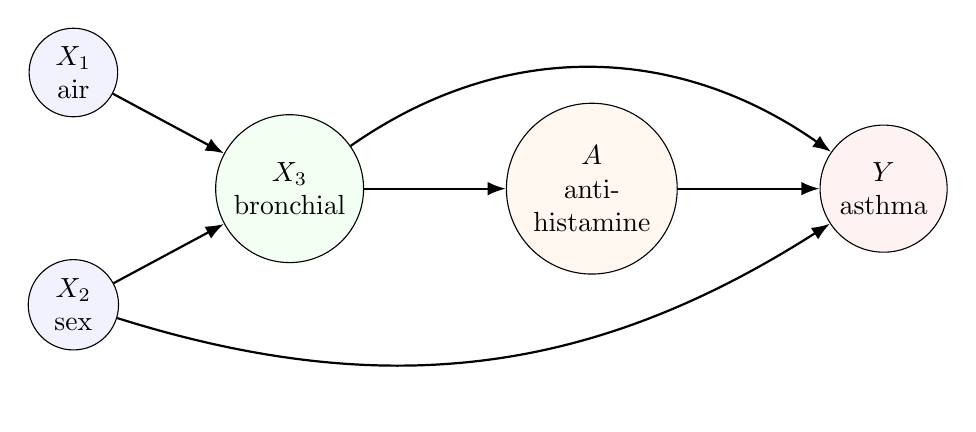
\begin{tikzpicture}[node distance=1.8cm,>=Latex]
  \node[draw, circle, fill=blue!5] (X1) {$X_1$\\air};
  \node[draw, circle, fill=blue!5, below=of X1] (X2) {$X_2$\\sex};
  \node[draw, circle, fill=green!5, right=1.8cm of $(X1)!0.5!(X2)$] (X3) {$X_3$\\bronchial};
  \node[draw, circle, fill=orange!6, right=of X3] (A) {$A$\\anti-\\histamine};
  \node[draw, circle, fill=red!5, right=of A] (Y) {$Y$\\asthma};
  \draw[->, thick] (X1) -- (X3);
  \draw[->, thick] (X2) -- (X3);
  \draw[->, thick] (X3) -- (A);
  \draw[->, thick]
  (X3) to[out=35,in=145]
  (Y);
  \draw[->, thick] (X2) to[bend right=25] (Y);
  \draw[->, thick] (A) -- (Y);
\end{tikzpicture}
\caption{A possible causal DAG for antihistamine treatment and asthma.}
\end{figure}

\subsection{Meaning of Absent Arrows}

Absent arrows are as important as present arrows. If a causal DAG omits $X\to Y$, it asserts that $X$ has no direct causal effect on $Y$ once the other variables in the graph are included.

For example, if the graph includes $X_1\to X_3\to Y$ but no $X_1\to Y$, it says that air pollution affects asthma only through the represented intermediate variables, not directly. This is a strong scientific claim.

If the analyst is unsure whether a direct effect exists, a conservative strategy is to leave the arrow in. Removing an arrow encodes knowledge; it should not be done merely to simplify the graph.

\subsection{DAGs as Scientific Assumptions}

A DAG is not estimated mechanically from the data in the ordinary causal workflow. It represents assumptions supplied by design knowledge and subject-matter reasoning. Data can sometimes contradict implications of a DAG, but many causal features of a DAG are not testable from observed data alone.

\begin{assumptionbox}
Using a causal DAG means accepting the causal claims encoded by its arrows and missing arrows. The graph is part of the causal model, not a decorative summary of associations.
\end{assumptionbox}

DAG construction should therefore be collaborative. Domain experts often know mechanisms that are invisible in a spreadsheet. A useful graph may also reveal discomfort: important variables were not measured, intervention timing is unclear, or some arrows cannot be confidently removed. That discomfort is scientifically productive because it clarifies what the data can and cannot support.

\lecture{2.4}{DAGs and Conditional Independencies}
\label{lec:2-4}

\subsection{DAG Factorization}

DAGs are useful because they connect causal structure to probabilistic structure. For any ordered variables $A,B,C,D,E$, the chain rule always gives
\[
\Prob(A,B,C,D,E)
=
\Prob(A)\Prob(B\given A)\Prob(C\given A,B)\Prob(D\given A,B,C)\Prob(E\given A,B,C,D).
\]
This identity is true for any joint distribution and does not require a graph.

Now consider the DAG
\[
A\to B,\quad A\to C,\quad B\to D,\quad C\to D,\quad D\to E.
\]
The parent sets are
\[
\pa(A)=\emptyset,\quad
\pa(B)=\{A\},\quad
\pa(C)=\{A\},\quad
\pa(D)=\{B,C\},\quad
\pa(E)=\{D\}.
\]
The DAG factorization is
\[
\Prob(A,B,C,D,E)
=
\Prob(A)\Prob(B\given A)\Prob(C\given A)\Prob(D\given B,C)\Prob(E\given D).
\]

\begin{definition}[DAG factorization]
A distribution is said to factorize according to a DAG if its joint density or mass function can be written as
\[
p(v)=\prod_{j=1}^m p(v_j\given \pa(v_j)),
\]
where $\pa(v_j)$ denotes the parents of node $V_j$ in the graph.
\end{definition}

When we use a DAG to read conditional independencies, we are assuming that the
relevant distribution is Markov with respect to the DAG, equivalently that it
satisfies this factorization.

\begin{figure}[H]
\centering
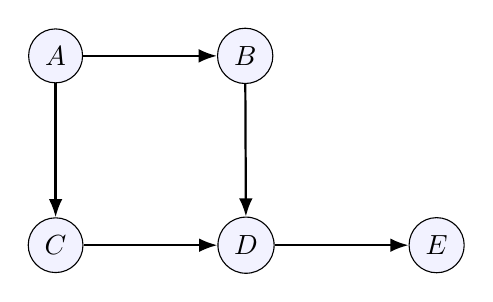
\begin{tikzpicture}[node distance=1.7cm,>=Latex]
  \node[draw, circle, fill=blue!5] (A) {$A$};
  \node[draw, circle, fill=blue!5, right=of A] (B) {$B$};
  \node[draw, circle, fill=blue!5, below=of A] (C) {$C$};
  \node[draw, circle, fill=blue!5, right=of C] (D) {$D$};
  \node[draw, circle, fill=blue!5, right=of D] (E) {$E$};
  \draw[->, thick] (A) -- (B);
  \draw[->, thick] (A) -- (C);
  \draw[->, thick] (B) -- (D);
  \draw[->, thick] (C) -- (D);
  \draw[->, thick] (D) -- (E);
\end{tikzpicture}
\caption{This DAG implies that each node's distribution depends on its parents, not on all earlier variables.}
\end{figure}

\subsection{Conditional Independence Implied by Missing Arrows}

The factorization above removes variables from conditioning sets. For example, the chain rule term
\[
\Prob(C\given A,B)
\]
is replaced by
\[
\Prob(C\given A).
\]
This replacement encodes
\[
C\ci B\given A.
\]
Similarly,
\[
\Prob(E\given A,B,C,D)=\Prob(E\given D)
\]
encodes that $E$ is conditionally independent of $A,B,C$ given $D$:
\[
E\ci (A,B,C)\given D.
\]

Under this Markov/factorization assumption, these conditional independencies
follow from missing arrows and the parent structure of the graph. Chapter 3 will
introduce d-separation, the graphical rule for reading such independencies
systematically.

\begin{keyidea}
A DAG does two things at once: it describes causal relationships and implies conditional independence restrictions on the joint distribution.
\end{keyidea}

\subsection{Including Measured and Unmeasured Variables}

A causal graph should not be restricted to variables that happen to appear in the data set. If an unmeasured factor affects both treatment and outcome, omitting it from the graph hides a threat to causal interpretation.

\begin{figure}[H]
\centering
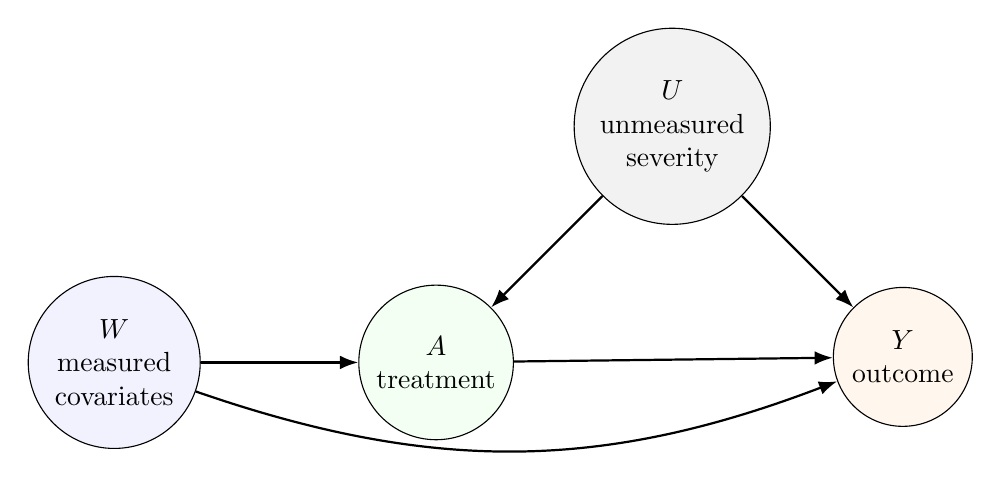
\begin{tikzpicture}[node distance=2.0cm,>=Latex]
  \node[draw, circle, fill=gray!10] (U) {$U$\\unmeasured\\severity};
  \node[draw, circle, fill=green!5, below left=of U] (A) {$A$\\treatment};
  \node[draw, circle, fill=orange!7, below right=of U] (Y) {$Y$\\outcome};
  \node[draw, circle, fill=blue!5, left=of A] (W) {$W$\\measured\\covariates};
  \draw[->, thick] (U) -- (A);
  \draw[->, thick] (U) -- (Y);
  \draw[->, thick] (W) -- (A);
  \draw[->, thick] (W) to[bend right=20] (Y);
  \draw[->, thick] (A) -- (Y);
\end{tikzpicture}
\caption{Unmeasured variables should appear in causal graphs when they are part of the scientific system.}
\end{figure}

The node $U$ may never be observed, but it matters. If severe symptoms drive both imaging and later disability, then a graph without $U$ may falsely suggest that measured covariates are sufficient for causal adjustment.

\subsection{Collapsing Variables into Nodes}

Sometimes a node represents a vector. For instance, $W$ may stand for age, sex, baseline pain score, comorbidities, insurance status, and prior utilization:
\[
W=(W_1,\ldots,W_p).
\]
This is convenient when the internal relationships among the $W_j$ variables are not central to the causal question.

Collapsing is inappropriate when the relationships inside the vector matter. If one component of $W$ is the exposure, mediator, or outcome, it should receive its own node. If temporal ordering among components matters, collapsing them can hide causal feedback.

\subsection{Representing Time to Avoid Cycles}

Many real systems appear cyclic when described coarsely. Infection can cause malnutrition, and malnutrition can increase susceptibility to infection. A DAG cannot contain a cycle, so the solution is to represent the process over time:
\[
\text{infection}_1 \to \text{malnutrition}_2 \to \text{infection}_3,
\]
and
\[
\text{malnutrition}_1 \to \text{infection}_2 \to \text{malnutrition}_3.
\]

\begin{figure}[H]
\centering
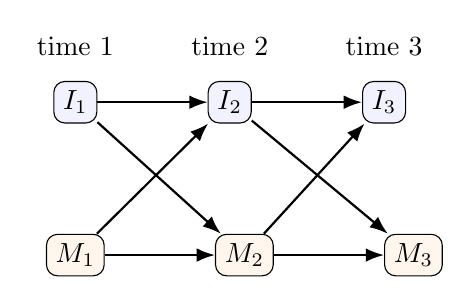
\begin{tikzpicture}[node distance=1.4cm,>=Latex]
  \node[draw, rounded corners, fill=blue!5] (I1) {$I_1$};
  \node[draw, rounded corners, fill=orange!7, below=of I1] (M1) {$M_1$};
  \node[draw, rounded corners, fill=blue!5, right=of I1] (I2) {$I_2$};
  \node[draw, rounded corners, fill=orange!7, right=of M1] (M2) {$M_2$};
  \node[draw, rounded corners, fill=blue!5, right=of I2] (I3) {$I_3$};
  \node[draw, rounded corners, fill=orange!7, right=of M2] (M3) {$M_3$};
  \draw[->, thick] (I1) -- (I2);
  \draw[->, thick] (I2) -- (I3);
  \draw[->, thick] (M1) -- (M2);
  \draw[->, thick] (M2) -- (M3);
  \draw[->, thick] (I1) -- (M2);
  \draw[->, thick] (M1) -- (I2);
  \draw[->, thick] (I2) -- (M3);
  \draw[->, thick] (M2) -- (I3);
  \node[above=.2cm of I1] {time 1};
  \node[above=.2cm of I2] {time 2};
  \node[above=.2cm of I3] {time 3};
\end{tikzpicture}
\caption{Feedback over time can be represented without cycles by indexing variables by time.}
\end{figure}

\subsection{Building DAGs with Subject-Matter Knowledge}

DAG building should start from the scientific system, not from the available columns in the data set. A useful workflow is:
\begin{enumerate}
  \item List the exposure, outcome, and variables known or suspected to affect either.
  \item Order variables temporally when possible.
  \item Begin with a rich graph containing plausible arrows.
  \item Remove an arrow only when there is a substantive reason to believe the direct effect is absent.
  \item Mark which variables are measured and which are unmeasured.
  \item Revisit the graph with subject-matter experts.
\end{enumerate}

If the graph shows that key variables were not measured, that is not a failure of graphing. It is useful information. The conclusion may be that the current study needs stronger assumptions, a different target question, sensitivity analysis, or more cautious interpretation as an association.

\lecture{2.5}{Counterfactual Variables}
\label{lec:2-5}

\subsection{Ideal Experiments}

A causal question is easiest to understand by first imagining an ideal experiment. Suppose we want to know whether early imaging affects 12-month back pain-related disability. In an ideal experiment with unlimited control, we could take the target population and create two worlds:
\begin{itemize}
  \item in one world, every eligible patient receives early imaging;
  \item in another world, no eligible patient receives early imaging.
\end{itemize}
We would then compare the outcomes in these two worlds.

This thought experiment is not meant to be physically possible. Its purpose is to clarify the intervention and the outcome. A causal question is a question about what would happen under actions, not merely about what happened under observed decisions.

\begin{figure}[H]
\centering
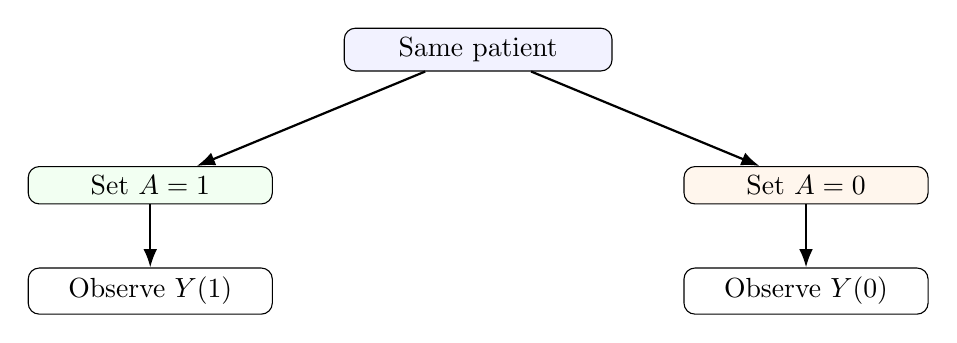
\begin{tikzpicture}[node distance=1.1cm,>=Latex]
  \node[draw, rounded corners, fill=blue!5, minimum width=3.4cm] (unit) {Same patient};
  \node[draw, rounded corners, fill=green!5, below left=1.2cm and .9cm of unit, minimum width=3.1cm] (a1) {Set $A=1$};
  \node[draw, rounded corners, fill=orange!7, below right=1.2cm and .9cm of unit, minimum width=3.1cm] (a0) {Set $A=0$};
  \node[draw, rounded corners, below=.8cm of a1, minimum width=3.1cm] (y1) {Observe $\Yone$};
  \node[draw, rounded corners, below=.8cm of a0, minimum width=3.1cm] (y0) {Observe $\Yzero$};
  \draw[->, thick] (unit) -- (a1);
  \draw[->, thick] (unit) -- (a0);
  \draw[->, thick] (a1) -- (y1);
  \draw[->, thick] (a0) -- (y0);
\end{tikzpicture}
\caption{Counterfactual thinking compares outcomes for the same unit under alternative interventions.}
\end{figure}

\subsection{Interventions}

\begin{definition}[Intervention]
An \emph{intervention} is an action or policy that sets, modifies, or otherwise changes a variable in the causal system. In notation, $\doop(A=a)$ denotes an intervention setting $A$ to value $a$.
\end{definition}

An intervention is not the same as conditioning. The expression $\E(Y\given A=a)$ describes the mean outcome among people who were observed with $A=a$. The expression $\E\{\Ya{a}\}$ describes the mean outcome that would be observed if the intervention set $A=a$ for the relevant population.

Conditioning selects a subgroup. Intervening changes the data-generating process.

\subsection{Potential Outcomes $\Ya{a}$}

\begin{definition}[Potential outcome]
For a treatment or exposure $A$ and outcome $Y$, the potential outcome $\Ya{a}$ is the outcome that would be observed for a unit under an intervention setting $A=a$.
\end{definition}

The notation $\Ya{a}$ is also called counterfactual notation. It is "counterfactual" when $a$ differs from the treatment value actually received, but it is useful to define potential outcomes for all intervention levels regardless of what was observed.

If $A$ is early imaging and $Y$ is 12-month disability, then:
\[
\Yone = \text{disability that would be observed if the patient received early imaging},
\]
\[
\Yzero = \text{disability that would be observed if the patient did not receive early imaging}.
\]

\subsection{Binary Treatment Potential Outcomes}

For a binary treatment $A\in\{0,1\}$, each unit has two potential outcomes:
\[
\Yzero,\qquad \Yone.
\]
The observed data contain only one observed outcome $Y$. If the patient actually received $A=1$, then under consistency we observe $\Yone$. If the patient actually received $A=0$, then we observe $\Yzero$. The other potential outcome remains unobserved.

\[
\begin{array}{c|ccc}
\text{patient} & A & \Yone & \Yzero\\
\hline
1 & 1 & 1 & 1\\
2 & 0 & 0 & 0\\
3 & 0 & 0 & 1\\
4 & 1 & 1 & 0\\
5 & 1 & 1 & 0
\end{array}
\]

The table is conceptual. In real observed data, both potential outcome columns are not jointly observed for every patient.

\subsection{No Interference}

The notation $\Ya{a}$ assumes that one unit's potential outcome depends only on that unit's assigned treatment level, not on treatments assigned to other units.

\begin{assumptionbox}
\textbf{No interference.} For unit $i$, the potential outcome under treatment $a$ is $Y_i(a)$ and does not depend on the treatment values assigned to other units:
\[
Y_i(a_1,\ldots,a_n)=Y_i(a_i)
\]
for all treatment vectors $(a_1,\ldots,a_n)$, whenever the simplified notation is used.
\end{assumptionbox}

Plainly, no interference says that my outcome under treatment does not change depending on your treatment.

\subsection{Interference Examples}

No interference can fail in infectious disease studies. Suppose households contain two people and $A_i$ indicates flu vaccination for person $i$. Person 1's flu infection outcome may depend on whether person 2 is vaccinated. Then the relevant potential outcome is
\[
Y_1(a_1,a_2),
\]
not merely $Y_1(a_1)$.

For a two-person household, the potential outcomes for person 1 might include
\[
Y_1(1,1),\quad Y_1(1,0),\quad Y_1(0,1),\quad Y_1(0,0).
\]
The second argument matters because vaccinating the housemate could reduce exposure to infection.

Interference can also arise through social networks, classrooms, neighborhoods, clinics, or markets. Vaccines, infectious disease transmission, peer education, and price interventions are common examples.

\subsection{Individual Causal Effects}

\begin{definition}[Individual causal effect]
For a binary treatment, an \emph{individual causal effect} is a contrast between the two potential outcomes for the same unit, such as
\[
Y_i(1)-Y_i(0)
\]
or, when meaningful,
\[
\frac{Y_i(1)}{Y_i(0)}.
\]
\end{definition}

For a binary adverse outcome, four qualitative types are possible:
\[
\begin{array}{c|ccc}
\text{type} & Y_i(1) & Y_i(0) & Y_i(1)-Y_i(0)\\
\hline
\text{doomed} & 1 & 1 & 0\\
\text{invincible} & 0 & 0 & 0\\
\text{helped} & 0 & 1 & -1\\
\text{harmed} & 1 & 0 & 1
\end{array}
\]
This table is conceptually useful, but it also reveals the central difficulty.

\subsection{Fundamental Problem of Causal Inference}

\begin{definition}[Fundamental problem of causal inference]
For a given unit at a given time, we can observe the outcome under the treatment actually received, but not under all alternative treatment levels. Therefore individual causal effects are generally not directly observable.
\end{definition}

If a patient receives early imaging, we observe the patient's outcome under imaging. We do not observe the same patient's outcome at the same time under no imaging. This is why causal inference usually targets population-level summaries rather than individual causal effects.

\begin{keyidea}
The causal problem is missing data at the level of potential outcomes. Each unit has multiple potential outcomes, but the observed data reveal at most one of them.
\end{keyidea}

\lecture{2.6}{Causal Parameters and Causal Effects}
\label{lec:2-6}

\subsection{Population-Level Causal Parameters}

Because individual causal effects are generally unobservable, causal inference usually focuses on population-level summaries of potential outcomes.

\begin{definition}[Population-level causal parameter]
A \emph{population-level causal parameter} is a summary of the distribution of one or more potential outcomes in a target population.
\end{definition}

Examples include:
\[
\E\{\Yone\},\qquad
\E\{\Yzero\},\qquad
\Prob(\Yone=1),\qquad
\operatorname{median}\{\Yone\}.
\]
These are not summaries of the observed treatment groups. They are summaries of outcomes under specified interventions.

\subsection{Average Causal Effect}

The most common causal effect compares average potential outcomes under two interventions.

\begin{definition}[Average causal effect]
For two treatment levels $a$ and $a'$, the \emph{average causal effect} on the additive scale is
\[
\E\{\Ya{a}\}-\E\{\Ya{a'}\}.
\]
\end{definition}

For the early imaging example, the average causal effect of imaging versus no imaging on disability is
\[
\E\{\Yone\}-\E\{\Yzero\}.
\]
If higher values of $Y$ indicate worse disability, then a positive value means the mean disability would be higher under early imaging than under no early imaging. A negative value means the mean disability would be lower under early imaging.

\subsection{Average Treatment Effect}

For binary treatment, the average causal effect is often called the average treatment effect.

\begin{definition}[Average treatment effect]
For binary treatment $A\in\{0,1\}$, the \emph{average treatment effect} is
\[
\ATE=\E(\Yone-\Yzero).
\]
When expectations are finite,
\[
\ATE=\E(\Yone)-\E(\Yzero).
\]
\end{definition}

The second equality is a consequence of linearity of expectation:
\[
\E(\Yone-\Yzero)
=\E(\Yone)+\E(-\Yzero)
=\E(\Yone)-\E(\Yzero).
\]
This equality is important because it shows that the ATE can be expressed using the two marginal mean potential outcomes.

\subsection{Marginal Distributions of Counterfactuals}

The ATE depends only on the marginal distributions of $\Yone$ and $\Yzero$. To see this, suppose the potential outcomes are discrete. Then
\[
\E(\Yone-\Yzero)
=
\sum_{y_0}\sum_{y_1}(y_1-y_0)
\Prob(\Yone=y_1,\Yzero=y_0).
\]
Distribute the sum:
\[
=
\sum_{y_0}\sum_{y_1}y_1\Prob(\Yone=y_1,\Yzero=y_0)
-
\sum_{y_0}\sum_{y_1}y_0\Prob(\Yone=y_1,\Yzero=y_0).
\]
For the first term, move $y_1$ outside the sum over $y_0$:
\[
\sum_{y_1}y_1\sum_{y_0}\Prob(\Yone=y_1,\Yzero=y_0)
=
\sum_{y_1}y_1\Prob(\Yone=y_1)
=
\E(\Yone).
\]
For the second term,
\[
\sum_{y_0}y_0\sum_{y_1}\Prob(\Yone=y_1,\Yzero=y_0)
=
\sum_{y_0}y_0\Prob(\Yzero=y_0)
=
\E(\Yzero).
\]
Therefore
\[
\E(\Yone-\Yzero)=\E(\Yone)-\E(\Yzero).
\]

\begin{identificationbox}
This derivation is not yet an identification result from observed data. It is a counterfactual distribution result: the additive ATE depends only on the marginal distributions of $\Yone$ and $\Yzero$, not on their joint distribution.
\end{identificationbox}

\subsection{Cross-World Quantities}

Some causal quantities depend on the joint distribution of potential outcomes under incompatible interventions. For example,
\[
\E\left(\frac{\Yone}{\Yzero}\right)
\]
requires the pair $(\Yone,\Yzero)$ for the same unit.

For discrete potential outcomes,
\[
\E\left(\frac{\Yone}{\Yzero}\right)
=
\sum_{y_0}\sum_{y_1}
\frac{y_1}{y_0}
\Prob(\Yone=y_1,\Yzero=y_0),
\]
when the ratio is well-defined. This expression depends on the joint probabilities $\Prob(\Yone=y_1,\Yzero=y_0)$, not merely the separate marginal distributions.

\subsection{Why Cross-World Assumptions Are Problematic}

The problem is that no ordinary experiment can observe both $\Yone$ and $\Yzero$ for the same unit at the same time. An experiment assigning everyone to $A=1$ can reveal features of the distribution of $\Yone$. An experiment assigning everyone to $A=0$ can reveal features of the distribution of $\Yzero$. Neither experiment reveals how $\Yone$ and $\Yzero$ are paired within individuals.

Any claim about their joint distribution requires assumptions linking outcomes across mutually exclusive worlds. These are called cross-world assumptions. Such assumptions may be mathematically convenient, but they are often difficult to justify scientifically.

\begin{keyidea}
Causal parameters based on marginal distributions of potential outcomes are usually preferable because they correspond more directly to ideal experiments. Parameters requiring the joint distribution of incompatible potential outcomes demand stronger cross-world assumptions.
\end{keyidea}

\subsection{Risk Differences, Ratios, and Other Contrasts}

When $Y$ is binary, $\E\{\Ya{a}\}=\Prob\{\Ya{a}=1\}$ is the risk under intervention $a$. Several contrasts are common:
\[
\text{Risk difference}=
\Prob(\Yone=1)-\Prob(\Yzero=1),
\]
\[
\text{Risk ratio}=
\frac{\Prob(\Yone=1)}{\Prob(\Yzero=1)},
\]
\[
\text{Odds ratio}=
\frac{\Prob(\Yone=1)/\Prob(\Yone=0)}
{\Prob(\Yzero=1)/\Prob(\Yzero=0)}.
\]

For continuous outcomes, one may compare means, medians, variances, quantiles, or probabilities of exceeding a clinically meaningful threshold:
\[
\Prob(\Yone>c)-\Prob(\Yzero>c).
\]
The best contrast depends on the scientific question, the outcome scale, and interpretability.

\lecture{2.7}{Marginal and Conditional Causal Effects}
\label{lec:2-7}

\subsection{Marginal ATE}

The marginal average treatment effect summarizes the effect in the entire target population:
\[
\ATE=\E(\Yone-\Yzero).
\]
It averages over all sources of variation in the population, including baseline covariates. In the early imaging example, the marginal ATE answers:
\begin{quote}
What is the average difference in disability if everyone in the target population received early imaging versus if no one received early imaging?
\end{quote}

The marginal ATE is often the primary public health or policy estimand because it describes the average impact of a population-level intervention.

\subsection{Conditional ATE}

A conditional average treatment effect restricts the comparison to a subgroup defined by covariates.

\begin{definition}[Conditional average treatment effect]
For covariates $W$, the \emph{conditional average treatment effect} at covariate value $w$ is
\[
\CATE(w)=\E(\Yone-\Yzero\given W=w).
\]
\end{definition}

If $W$ is baseline pain severity, then $\CATE(w)$ is the average effect of early imaging among patients with baseline pain severity $w$.

\subsection{Subgroup-Specific Causal Effects}

Subgroup-specific causal effects are conditional effects for scientifically meaningful groups. If $W$ is categorical, such as low, moderate, and severe baseline pain, then
\[
\E(\Yone-\Yzero\given W=\text{severe})
\]
is the ATE among patients with severe baseline pain.

The marginal ATE is a weighted average of conditional ATEs:
\[
\ATE
=\E\{\E(\Yone-\Yzero\given W)\}.
\]
For discrete $W$,
\[
\ATE
=
\sum_w \E(\Yone-\Yzero\given W=w)\Prob(W=w).
\]
This is the tower rule applied to the individual-level contrast $\Yone-\Yzero$.

\subsection{Causal Effect Modification}

\begin{definition}[Causal effect modification]
There is \emph{causal effect modification} by $W$ on the additive scale if
\[
\E(\Yone-\Yzero\given W=w)
\]
varies with $w$.
\end{definition}

For example, early imaging might have little average effect among patients with mild baseline pain but a different effect among patients with severe neurological symptoms. If the conditional causal effect differs across baseline severity levels, severity modifies the causal effect.

\begin{example}[A finite population]
Suppose a population of ten individuals has potential outcomes shown below.
\[
\begin{array}{c|ccc|c}
\text{ID} & W & \Yone & \Yzero & \Yone-\Yzero\\
\hline
1 & 2 & 2 & 3 & -1\\
2 & 1 & 10 & 5 & 5\\
3 & 1 & 8 & 7 & 1\\
4 & 1 & 6 & 3 & 3\\
5 & 0 & 2 & 0 & 2\\
6 & 2 & 3 & 6 & -3\\
7 & 0 & 4 & 0 & 4\\
8 & 1 & 0 & 5 & -5\\
9 & 2 & 7 & 0 & 7\\
10 & 0 & 6 & 9 & -3
\end{array}
\]
The marginal ATE is the average of the ten individual contrasts:
\[
\ATE=\frac{-1+5+1+3+2-3+4-5+7-3}{10}=1.
\]
The conditional effects are
\[
\CATE(0)=\frac{2+4-3}{3}=1,
\]
\[
\CATE(1)=\frac{5+1+3-5}{4}=1,
\]
\[
\CATE(2)=\frac{-1-3+7}{3}=1.
\]
In this example the marginal and subgroup effects are all equal on the additive scale, so there is no additive effect modification by $W$.
\end{example}

\subsection{Difference between Statistical Interaction and Causal Effect Heterogeneity}

Statistical interaction refers to variation in an observed-data association across levels of a covariate. For example, a regression model might show that
\[
\E(Y\given A=1,W=w)-\E(Y\given A=0,W=w)
\]
varies with $w$.

Causal effect heterogeneity refers to variation in a counterfactual contrast:
\[
\E(\Yone-\Yzero\given W=w).
\]
These are not the same object. Observed statistical interactions can arise from confounding, selection, measurement, or model scale. Conversely, causal effect heterogeneity can exist even when a particular regression model fails to show an interaction.

\begin{keyidea}
Effect modification is scale-specific and causal. It concerns whether a causal contrast, such as a risk difference or mean difference, varies across subgroups.
\end{keyidea}

\lecture{2.8}{From DAGs to SWIGs}
\label{lec:2-8}

\subsection{Single World Intervention Graphs}

DAGs represent causal relationships among observed or naturally occurring variables. Potential outcomes such as $\Ya{a}$ do not appear directly on an ordinary DAG. Single World Intervention Graphs, or SWIGs, extend DAGs so that counterfactual variables can be represented graphically.

\begin{definition}[Single World Intervention Graph]
A \emph{Single World Intervention Graph} is a graph obtained from a causal DAG by splitting intervention nodes into a random part and a fixed intervention part, then relabeling downstream variables as counterfactual variables under that intervention.
\end{definition}

"Single world" emphasizes that the graph represents one intervention world at a time. A SWIG for $A=1$ and a SWIG for $A=0$ are distinct intervention worlds.

\subsection{Splitting Treatment Nodes}

Suppose the original DAG is
\[
W\to A\to Y,\qquad W\to Y.
\]
To construct the SWIG for intervention $A=a$, split the node $A$ into:
\begin{itemize}
  \item a random part $A$, representing the treatment the unit would naturally receive;
  \item a fixed part $a$, representing the value imposed by intervention.
\end{itemize}
Incoming arrows into $A$ go to the random part. Outgoing arrows from $A$ leave the fixed part.

\begin{figure}[H]
\centering
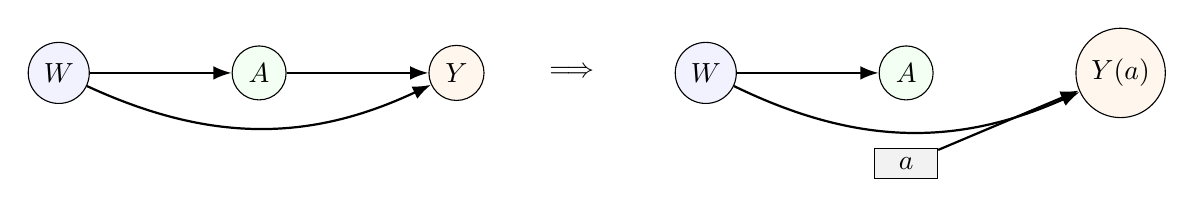
\begin{tikzpicture}[node distance=1.8cm,>=Latex]
  \node[draw, circle, fill=blue!5] (W1) {$W$};
  \node[draw, circle, fill=green!5, right=of W1] (A1) {$A$};
  \node[draw, circle, fill=orange!7, right=of A1] (Y1) {$Y$};
  \draw[->, thick] (W1) -- (A1);
  \draw[->, thick] (A1) -- (Y1);
  \draw[->, thick] (W1) to[bend right=25] (Y1);
  \node[right=.7cm of Y1] (arrow) {$\Longrightarrow$};
  \node[draw, circle, fill=blue!5, right=.9cm of arrow] (W2) {$W$};
  \node[draw, circle, fill=green!5, right=of W2] (A2) {$A$};
  \node[draw, rectangle, fill=gray!10, below=.6cm of A2, minimum width=.8cm] (a) {$a$};
  \node[draw, circle, fill=orange!7, right=of A2] (Y2) {$\Ya{a}$};
  \draw[->, thick] (W2) -- (A2);
  \draw[->, thick] (a) -- (Y2);
  \draw[->, thick] (W2) to[bend right=25] (Y2);
\end{tikzpicture}
\caption{A DAG is converted to a SWIG by splitting the intervened treatment node.}
\end{figure}

\subsection{Fixed Intervention Nodes}

The fixed node $a$ is not random. It represents the intervention value. Because it is fixed by the analyst's hypothetical intervention, it has no probability distribution in the intervention world.

The fixed node inherits outgoing arrows from the original treatment node. If $A$ had an arrow to $Y$ in the DAG, then $a$ has an arrow to $\Ya{a}$ in the SWIG. If $A$ had an arrow to a mediator $M$, then $a$ has an arrow to the counterfactual mediator $\M(a)$.

\subsection{Random Counterfactual Nodes}

Downstream nodes are relabeled as counterfactuals. If $Y$ is downstream of $A$, then under intervention $A=a$ the outcome node becomes $\Ya{a}$. If $M$ is downstream of $A$, it becomes $M(a)$.

Nodes not downstream of the intervention keep their original labels. In the graph above, $W$ is a baseline covariate before $A$, so it remains $W$.

\subsection{Constructing SWIGs from DAGs}

The construction rule is:
\begin{enumerate}
  \item Start with a causal DAG.
  \item Choose the node or nodes to intervene on.
  \item Split each intervention node into a random part and fixed part.
  \item Send incoming arrows to the random part.
  \item Send outgoing arrows from the fixed part.
  \item Relabel downstream nodes as counterfactual variables under the intervention.
\end{enumerate}

For a mediation DAG $A\to M\to Y$ with also $A\to Y$, intervening on $A=a$ gives:

\begin{figure}[H]
\centering
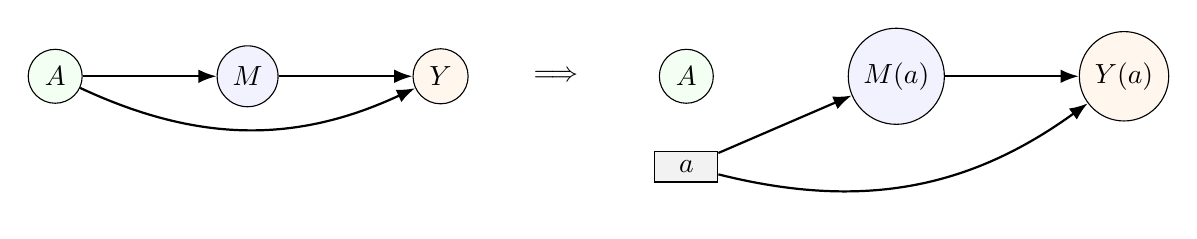
\begin{tikzpicture}[node distance=1.7cm,>=Latex]
  \node[draw, circle, fill=green!5] (A) {$A$};
  \node[draw, circle, fill=blue!5, right=of A] (M) {$M$};
  \node[draw, circle, fill=orange!7, right=of M] (Y) {$Y$};
  \draw[->, thick] (A) -- (M);
  \draw[->, thick] (M) -- (Y);
  \draw[->, thick] (A) to[bend right=25] (Y);
  \node[right=.7cm of Y] (arr) {$\Longrightarrow$};
  \node[draw, circle, fill=green!5, right=.9cm of arr] (Ar) {$A$};
  \node[draw, rectangle, fill=gray!10, below=.6cm of Ar, minimum width=.8cm] (a) {$a$};
  \node[draw, circle, fill=blue!5, right=of Ar] (Ma) {$M(a)$};
  \node[draw, circle, fill=orange!7, right=of Ma] (Ya) {$Y(a)$};
  \draw[->, thick] (a) -- (Ma);
  \draw[->, thick] (Ma) -- (Ya);
  \draw[->, thick] (a) to[bend right=25] (Ya);
\end{tikzpicture}
\caption{A mediation DAG and the SWIG under intervention $A=a$.}
\end{figure}

If we intervene on both treatment and mediator, setting $A=a$ and $M=m$, the downstream outcome becomes $Y(a,m)$.

\subsection{Reading Counterfactual Quantities from SWIGs}

SWIGs help identify which counterfactual variables are generated by a particular intervention. In the simple treatment graph, the SWIG for $A=a$ contains $\Ya{a}$, so $\E\{\Ya{a}\}$ is a natural causal parameter.

In the mediation graph, the SWIG for $A=a$ contains $M(a)$ and $Y(a)$. A SWIG for the joint intervention $(A=a,M=m)$ contains $Y(a,m)$. These are different causal questions:
\[
Y(a) \quad\text{allows the mediator to respond naturally to } A=a,
\]
whereas
\[
Y(a,m) \quad\text{sets both treatment and mediator}.
\]

\begin{keyidea}
SWIGs make the intervention explicit. Different interventions on the same original DAG can generate different counterfactual variables and therefore different causal questions.
\end{keyidea}

\lecture{2.9}{Types of Interventions and Consistency}
\label{lec:2-9}

\subsection{Static Interventions}

The simplest interventions are static interventions.

\begin{definition}[Static intervention]
A \emph{static intervention} assigns the same fixed treatment value or treatment regime to every unit in the target population.
\end{definition}

For a binary point treatment, examples are:
\[
\doop(A=1): \text{ assign everyone to treatment},
\]
\[
\doop(A=0): \text{ assign everyone to no treatment}.
\]
The corresponding potential outcomes are $\Yone$ and $\Yzero$.

Not all interventions are static. A stochastic intervention assigns treatment according to a specified probability distribution. A dynamic intervention assigns treatment according to a rule depending on a person's evolving history. For example, an HIV treatment rule might switch therapy when CD4 count falls below a threshold.

\subsection{Well-Defined Interventions}

A causal question is only as clear as its intervention.

\begin{definition}[Well-defined intervention]
An intervention is \emph{well-defined} if it specifies the action sufficiently clearly that the relevant potential outcome has a stable meaning across units and settings.
\end{definition}

"Early imaging" may be ambiguous. Does it mean recommending imaging, ordering imaging, completing imaging, obtaining MRI only, obtaining any lumbar imaging, or ensuring imaging within a particular number of days? These versions may have different effects.

Similarly, "the effect of BMI" is ambiguous unless the intervention is specified. Reducing BMI by diet, exercise, medication, or surgery may have different biological and social consequences. A causal question should describe the action, not only the variable label.

\begin{assumptionbox}
When using potential outcome notation $\Ya{a}$, we assume that the intervention level $a$ is defined clearly enough that the counterfactual outcome is meaningful. Ambiguous treatment versions can make consistency and interpretation fail.
\end{assumptionbox}

\subsection{Hypothetical Interventions}

Some interventions are hypothetical but still useful. A policy may not yet exist, or a trial may not be feasible, but the intervention can be described coherently enough to define a causal parameter.

For example, one might ask what would happen if all eligible patients received a reminder phone call, even if such a reminder system has not yet been implemented. The intervention is hypothetical but imaginable.

Other questions are more difficult. Asking for "the causal effect of race" is problematic if no well-defined intervention on race is specified. More precise questions may target interventions on discriminatory treatment, names on resumes, neighborhood assignment, income, educational access, or other manipulable social conditions. These questions may not capture every meaning of race, but they define clearer intervention contrasts.

\subsection{Manipulability}

Some scholars argue that causal effects should be defined only for variables that are manipulable. Others allow causal questions about nonmanipulable attributes if the counterfactual contrast is scientifically meaningful and carefully interpreted.

The practical lesson is not that every variable must be physically manipulable in a laboratory. The lesson is that the analyst must say what intervention, policy, or hypothetical change gives meaning to the potential outcome.

\begin{keyidea}
Causal inference is about effects of interventions. When the intervention is vague, the causal parameter is vague.
\end{keyidea}

\subsection{Causal Consistency}

Consistency links potential outcomes to observed outcomes.

\begin{assumptionbox}
\textbf{Causal consistency.} If a unit is observed to receive treatment level $A=a$, then its observed outcome equals its potential outcome under that treatment level:
\[
Y=\Ya{a}\quad\text{for units with }A=a.
\]
For binary treatment, this can be written as
\[
Y=A\Yone+(1-A)\Yzero.
\]
\end{assumptionbox}

The binary formula is worth unpacking. If $A=1$, then
\[
A\Yone+(1-A)\Yzero=1\cdot \Yone+0\cdot \Yzero=\Yone.
\]
If $A=0$, then
\[
A\Yone+(1-A)\Yzero=0\cdot \Yone+1\cdot \Yzero=\Yzero.
\]
Thus the formula says exactly that the observed outcome is the potential outcome corresponding to the treatment actually received.

\begin{example}[Observed and ideal data]
In an ideal data table for binary treatment, each patient has $A$, $\Yzero$, and $\Yone$:
\[
\begin{array}{c|ccc}
\text{ID} & A & \Yzero & \Yone\\
\hline
1 & 1 & 1 & 0\\
2 & 0 & 0 & 0\\
3 & 0 & 1 & 1\\
4 & 1 & 0 & 1
\end{array}
\]
The observed data contain $A$ and $Y$:
\[
\begin{array}{c|cc}
\text{ID} & A & Y\\
\hline
1 & 1 & 0\\
2 & 0 & 0\\
3 & 0 & 1\\
4 & 1 & 1
\end{array}
\]
For each row, the observed $Y$ equals the potential outcome under the observed treatment.
\end{example}

\subsection{Statistical Consistency vs Causal Consistency}

Causal consistency is different from statistical consistency. Statistical consistency is a property of an estimator:
\[
\hat\psi_n \overset{P}{\longrightarrow} \psi.
\]
It says that, with increasing sample size, the estimator approaches the target parameter.

Causal consistency is an assumption about the relationship between observed outcomes and potential outcomes. It says that the observed outcome under the observed treatment agrees with the corresponding counterfactual outcome.

The two ideas share a word but belong to different parts of the roadmap. Statistical consistency concerns estimation. Causal consistency concerns the definition and linkage of causal and observed data.

\subsection{Measured and Unmeasured Variables}

Before assessing whether a causal parameter can be identified, the analyst must mark which variables in the causal model are measured. A SWIG or DAG may include:
\begin{itemize}
  \item measured baseline covariates $W$;
  \item measured treatment $A$;
  \item measured outcome $Y$;
  \item unmeasured common causes $U$;
  \item post-treatment variables $Z$ or mediators $M$.
\end{itemize}

\begin{figure}[H]
\centering
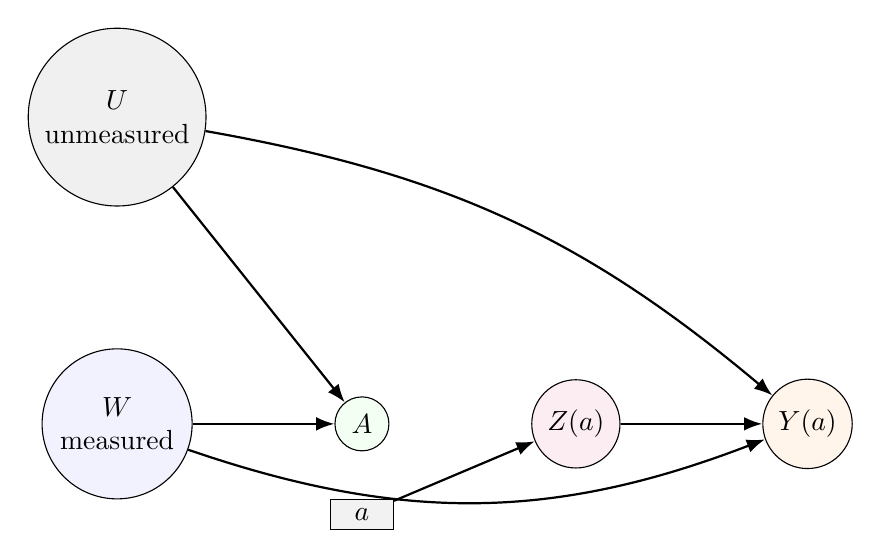
\begin{tikzpicture}[node distance=1.8cm,>=Latex]
  \node[draw, circle, fill=blue!5] (W) {$W$\\measured};
  \node[draw, circle, fill=gray!12, above=of W] (U) {$U$\\unmeasured};
  \node[draw, circle, fill=green!5, right=of W] (A) {$A$};
  \node[draw, rectangle, fill=gray!10, below=.6cm of A, minimum width=.8cm] (a) {$a$};
  \node[draw, circle, fill=purple!7, right=of A] (Z) {$Z(a)$};
  \node[draw, circle, fill=orange!8, right=of Z] (Y) {$Y(a)$};
  \draw[->, thick] (W) -- (A);
  \draw[->, thick] (U) -- (A);
  \draw[->, thick] (U) to[bend left=15] (Y);
  \draw[->, thick] (W) to[bend right=20] (Y);
  \draw[->, thick] (a) -- (Z);
  \draw[->, thick] (Z) -- (Y);
\end{tikzpicture}
\caption{A SWIG can distinguish measured covariates, unmeasured variables, fixed interventions, and counterfactual descendants.}
\end{figure}

This distinction will matter for identification. If all common causes of treatment and outcome are measured, one set of identification strategies may be plausible. If important common causes are unmeasured, different strategies or stronger assumptions may be required.

\begin{keyidea}
Chapter 2 defines the language of causal questions: interventions, potential outcomes, causal parameters, graphs, SWIGs, and consistency. Chapter 3 asks when these causal quantities can be learned from observed data.
\end{keyidea}


\chapterheading{3}{Identification of Causal Parameters and the ATE}
\lecture{3.1}{What Is Causal Identification?}
\label{lec:3-1}

\subsection{Counterfactual Distribution vs Observed Data Distribution}

Chapter 2 introduced causal parameters as summaries of counterfactual variables. For a binary treatment $A$, the average treatment effect is
\[
\ATE=\E(\Yone-\Yzero)=\E(\Yone)-\E(\Yzero).
\]
This parameter is defined in terms of the joint scientific object containing potential outcomes. The observed data, however, usually have the form
\[
O=(W,A,Y),
\]
where $W$ denotes measured covariates, $A$ the treatment actually received, and $Y$ the outcome actually observed.

\begin{definition}[Counterfactual distribution]
The \emph{counterfactual distribution} is the probability distribution of variables such as $\Yzero$, $\Yone$, and possibly other counterfactual quantities under interventions.
\end{definition}

\begin{definition}[Observed data distribution]
The \emph{observed data distribution} is the probability distribution of the variables actually measured in the study, such as $P(W,A,Y)$.
\end{definition}

These are different objects. The causal parameter $\E(\Yone)$ lives in the counterfactual distribution. A statistical parameter such as $\E\{\E(Y\given A=1,W)\}$ lives in the observed data distribution.

\subsection{Identification as a Bridge}

Identification asks whether a causal parameter can be rewritten using only the observed data distribution, under clearly stated assumptions.

\begin{definition}[Causal identification]
A causal parameter $\psi$ is \emph{identified} under a causal model if $\psi$ is equal to a functional of the observed data distribution $P(O)$ for every data-generating process satisfying the assumptions in that causal model.
\end{definition}

Informally, identification means we can write an equality of the form
\[
\text{counterfactual quantity}
\quad
\overset{\text{assumptions}}{=}
\quad
\text{observed-data quantity}.
\]
For example, later in this chapter we will derive
\[
\E\{\Ya{a}\}
=
\E\{\E(Y\given A=a,W)\},
\]
under consistency, conditional randomization, and positivity. The left side is causal. The right side is a statistical parameter of the observed distribution.

\begin{figure}[H]
\centering
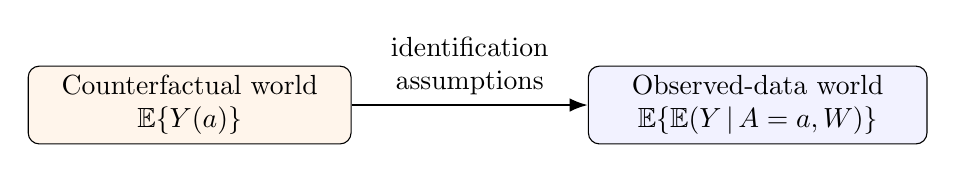
\begin{tikzpicture}[node distance=3cm,>=Latex]
  \node[draw, rounded corners, fill=orange!8, minimum width=4.1cm] (cf) {Counterfactual world\\$\E\{\Ya{a}\}$};
  \node[draw, rounded corners, fill=blue!5, right=of cf, minimum width=4.3cm] (obs) {Observed-data world\\$\E\{\E(Y\given A=a,W)\}$};
  \draw[->, thick] (cf) -- node[above]{identification\\assumptions} (obs);
\end{tikzpicture}
\caption{Identification connects a causal estimand to an observed-data parameter.}
\end{figure}

\subsection{Identifiability in the Causal Roadmap}

Identification is the fourth step in the causal roadmap:
\begin{enumerate}
  \item specify a causal model;
  \item specify a causal question and causal parameter;
  \item specify observed data and link them to the causal model;
  \item assess identifiability;
  \item specify a statistical parameter and model;
  \item estimate;
  \item interpret.
\end{enumerate}

The ordering matters. Before estimating, we must know what observed-data parameter represents the causal parameter. Otherwise we may estimate a precise but irrelevant quantity.

\begin{identificationbox}
Identification is a large-sample, infinite-data question. It asks: if we knew the entire observed data distribution exactly, could we determine the causal parameter under the stated assumptions?
\end{identificationbox}

\subsection{Why Identification Precedes Estimation}

Estimation concerns finite-sample uncertainty. Identification concerns whether the target is learnable from the observed data distribution at all. If a causal parameter is not identified, collecting more observations from the same observed data distribution does not solve the problem. Infinite data would reveal the observed distribution perfectly, but the causal parameter could still remain ambiguous.

This distinction is central:
\begin{itemize}
  \item \emph{Identification problem}: the observed data do not contain enough information, under current assumptions, to determine the causal parameter.
  \item \emph{Estimation problem}: the causal parameter has been written as an observed-data parameter, and we need to estimate it from a finite sample.
\end{itemize}

Machine learning can help estimate complex functions such as $\E(Y\given A,W)$ or $\Prob(A=1\given W)$. It cannot, by itself, create identification. Identification comes from the causal model and assumptions.

\begin{keyidea}
Identification tells us what to estimate. Estimation tells us how to approximate that identified statistical target using finite data.
\end{keyidea}

\lecture{3.2}{Confounding and Exchangeability}
\label{lec:3-2}

\subsection{Classical Confounder Definition}

The classical epidemiologic description says that a confounder is a variable associated with both exposure and outcome, and not on the causal pathway from exposure to outcome. For example, baseline disease severity may affect both whether a patient receives a risky cancer treatment and whether the patient dies of cancer. Disease severity can therefore confound the treatment-outcome association.

\begin{figure}[H]
\centering
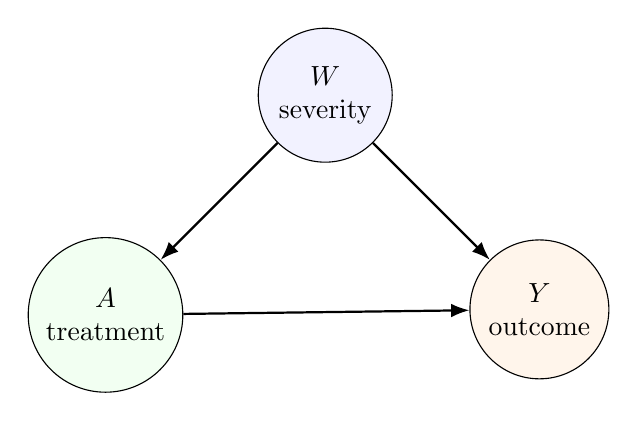
\begin{tikzpicture}[node distance=2.1cm,>=Latex]
  \node[draw, circle, fill=blue!5] (W) {$W$\\severity};
  \node[draw, circle, fill=green!5, below left=of W] (A) {$A$\\treatment};
  \node[draw, circle, fill=orange!8, below right=of W] (Y) {$Y$\\outcome};
  \draw[->, thick] (W) -- (A);
  \draw[->, thick] (W) -- (Y);
  \draw[->, thick] (A) -- (Y);
\end{tikzpicture}
\caption{A classical confounding structure: $W$ is a common cause of treatment and outcome.}
\end{figure}

This definition is useful but incomplete. In complex problems, variables can be time-varying, affected by prior treatment, measured with error, or unmeasured. A more general definition uses counterfactual independence.

\subsection{Counterfactual Independence Definition}

\begin{definition}[No unmeasured confounding for a point treatment]
For a binary treatment $A$, there is no unmeasured confounding given covariates $W$ if
\[
\Yzero \ci A \given W
\qquad\text{and}\qquad
\Yone \ci A \given W.
\]
Equivalently, for $a\in\{0,1\}$,
\[
\Ya{a}\ci A\given W.
\]
\end{definition}

In words, among people with the same covariates $W$, the treatment actually received carries no additional information about the potential outcomes. Within covariate strata, treated and untreated people are exchangeable with respect to what would happen under either treatment.

\subsection{Randomization}

In an ideal randomized trial, treatment assignment is generated by a random device that does not use patient prognosis. If treatment is randomized unconditionally, then
\[
\Yzero \ci A
\qquad\text{and}\qquad
\Yone \ci A.
\]
This means that the treated and untreated groups have the same distribution of potential outcomes before treatment is assigned, up to random sampling variation.

\begin{assumptionbox}
\textbf{Randomization condition.} For a binary point treatment,
\[
\Ya{a}\ci A,\qquad a=0,1.
\]
Plainly, treatment assignment gives no information about what the outcome would be under either treatment level.
\end{assumptionbox}

\subsection{Conditional Randomization}

In observational studies, unconditional randomization is usually implausible. Treatment decisions often depend on covariates. A weaker assumption is that treatment is randomized within strata of measured covariates:
\[
\Ya{a}\ci A\given W,\qquad a=0,1.
\]

This is plausible when $W$ contains all common causes of treatment and outcome needed to make treatment assignment as-if random. For example, if physicians choose early imaging based on baseline pain, neurological symptoms, age, cancer history, and prior utilization, then those variables must be included in $W$ for conditional randomization to be plausible.

\begin{assumptionbox}
\textbf{Conditional randomization.} For every treatment level $a$,
\[
\Ya{a}\ci A\given W.
\]
This says treatment is as-if randomized among people with the same $W$.
\end{assumptionbox}

\subsection{Ignorability}

The terms \emph{ignorability}, \emph{conditional ignorability}, and \emph{no unmeasured confounding} are often used for the same counterfactual independence condition. The idea is that after conditioning on $W$, the treatment assignment mechanism can be ignored for the purpose of identifying the distribution of $\Ya{a}$.

The word "ignored" should not be misunderstood. We do not ignore treatment assignment in estimation. Rather, the assumption says that the remaining dependence between treatment and potential outcomes has been removed by conditioning on $W$.

\subsection{Exchangeability}

Exchangeability is another name for the same idea, emphasizing comparability of groups.

\begin{definition}[Exchangeability]
Treated and untreated groups are \emph{exchangeable} with respect to potential outcomes, possibly conditional on $W$, if their potential outcome distributions are the same:
\[
\Ya{a}\ci A\given W.
\]
\end{definition}

If exchangeability holds, then within a stratum $W=w$, the observed outcomes among people with $A=a$ can represent the potential outcomes under $a$ for everyone in that stratum.

\subsection{Why Ignorability Cannot Be Empirically Verified}

Ignorability involves potential outcomes that are not jointly observed. Among treated people we observe outcomes under treatment, but not what their outcomes would have been without treatment. Among untreated people we observe outcomes without treatment, but not what their outcomes would have been under treatment.

Therefore, the condition
\[
\Ya{a}\ci A\given W
\]
cannot be tested directly from the observed data. We can check whether measured covariates are balanced across treatment groups. We can check whether some covariates predict treatment. But we cannot check whether all unmeasured causes of the outcome have been controlled.

\begin{keyidea}
Exchangeability is a causal assumption, not an empirical fact discovered by a balance table. Balance diagnostics can reveal problems, but they cannot prove that ignorability holds.
\end{keyidea}

\lecture{3.3}{d-Separation in DAGs}
\label{lec:3-3}

\subsection{Paths}

d-Separation is a graphical rule for reading conditional independence statements
from a DAG. It answers questions such as whether $X\ci Y\given Z$ is implied by
a graph, under the assumption that the distribution is Markov with respect to the
DAG.

\begin{definition}[Path]
A \emph{path} between two nodes is a sequence of adjacent nodes connecting them, with no node repeated. The arrows on the path do not need to point in the same direction.
\end{definition}

For example, in $A\to B\to D\leftarrow F$, the sequence $A,B,D,F$ is a path from $A$ to $F$, even though the last arrow points into $D$.

\subsection{Forks}

A fork has the form
\[
X\leftarrow Z\to Y.
\]
Here $Z$ is a common cause of $X$ and $Y$.

\begin{figure}[H]
\centering
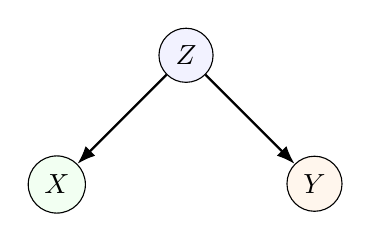
\begin{tikzpicture}[node distance=1.6cm,>=Latex]
  \node[draw, circle, fill=blue!5] (Z) {$Z$};
  \node[draw, circle, fill=green!5, below left=of Z] (X) {$X$};
  \node[draw, circle, fill=orange!7, below right=of Z] (Y) {$Y$};
  \draw[->, thick] (Z) -- (X);
  \draw[->, thick] (Z) -- (Y);
\end{tikzpicture}
\caption{A fork: $X$ and $Y$ share a common cause $Z$.}
\end{figure}

Forks are open unless we condition on the middle node. Thus typically
\[
X\nci Y,
\qquad
X\ci Y\given Z
\]
as implied by this simple graph. Intuitively, warm weather may cause both ice cream sales and visits to the beach. Conditioning on weather removes the common-cause explanation for their association.

\subsection{Chains}

A chain has the form
\[
X\to Z\to Y
\]
or
\[
X\leftarrow Z\leftarrow Y.
\]
The middle node transmits association along a directed pathway.

\begin{figure}[H]
\centering
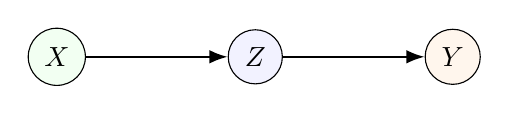
\begin{tikzpicture}[node distance=1.8cm,>=Latex]
  \node[draw, circle, fill=green!5] (X) {$X$};
  \node[draw, circle, fill=blue!5, right=of X] (Z) {$Z$};
  \node[draw, circle, fill=orange!7, right=of Z] (Y) {$Y$};
  \draw[->, thick] (X) -- (Z);
  \draw[->, thick] (Z) -- (Y);
\end{tikzpicture}
\caption{A chain: association flows through the middle node $Z$.}
\end{figure}

Chains are open unless we condition on the middle node:
\[
X\nci Y,
\qquad
X\ci Y\given Z.
\]
If $X$ affects $Y$ only through $Z$, then once $Z$ is known, $X$ provides no additional information about $Y$.

\subsection{Colliders}

A collider has the form
\[
X\to Z\leftarrow Y.
\]
The arrows on the path collide at $Z$.

\begin{figure}[H]
\centering
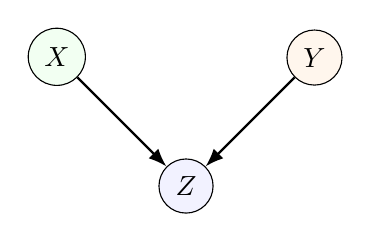
\begin{tikzpicture}[node distance=1.6cm,>=Latex]
  \node[draw, circle, fill=blue!5] (Z) {$Z$};
  \node[draw, circle, fill=green!5, above left=of Z] (X) {$X$};
  \node[draw, circle, fill=orange!7, above right=of Z] (Y) {$Y$};
  \draw[->, thick] (X) -- (Z);
  \draw[->, thick] (Y) -- (Z);
\end{tikzpicture}
\caption{A collider: $Z$ is a common effect of $X$ and $Y$.}
\end{figure}

Colliders behave differently from forks and chains. A collider blocks the path unless we condition on the collider or one of its descendants:
\[
X\ci Y,
\qquad
X\nci Y\given Z.
\]
For example, a car failing to start may be caused by a dead battery or an empty fuel tank. Before knowing whether the car starts, battery status and fuel status might be independent. After learning the car failed to start, evidence that the battery is fine makes an empty fuel tank more likely.

\subsection{Collider Descendants}

Conditioning on a descendant of a collider can also open the path. If
\[
X\to Z\leftarrow Y,\qquad Z\to D,
\]
then conditioning on $D$ can induce dependence between $X$ and $Y$.

The reason is that $D$ carries information about the collider $Z$. If $D$ is "taken to the mechanic" and $Z$ is "car fails to start," then observing $D$ gives partial information about $Z$, which can create dependence between the causes of $Z$.

\subsection{Blocking and Opening Paths}

A path is blocked by a conditioning set $S$ if at least one of the following occurs:
\begin{itemize}
  \item the path contains a chain or fork whose middle node is in $S$;
  \item the path contains a collider such that neither the collider nor any descendant of the collider is in $S$.
\end{itemize}

Equivalently:
\begin{itemize}
  \item conditioning on non-colliders blocks paths;
  \item conditioning on colliders or their descendants opens paths.
\end{itemize}

\subsection{d-Separation Rules}

\begin{definition}[d-separation]
Two nodes $X$ and $Y$ are \emph{d-separated} by a set $S$ if every path between $X$ and $Y$ is blocked by $S$. If at least one path remains open, $X$ and $Y$ are \emph{d-connected} given $S$.
\end{definition}

If a DAG represents the data-generating process and $X$ and $Y$ are d-separated by $S$, then the graph implies
\[
X\ci Y\given S.
\]

\subsection{Practice Examples}

Consider the DAG:
\[
A\to B,\quad A\to C,\quad B\to D,\quad C\to D,\quad F\to D,\quad D\to E.
\]

\begin{figure}[H]
\centering
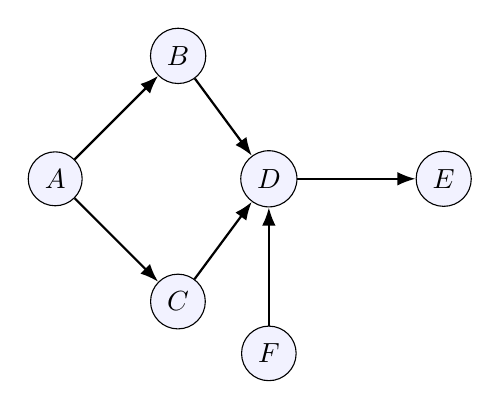
\begin{tikzpicture}[node distance=1.5cm,>=Latex]
  \node[draw, circle, fill=blue!5] (A) {$A$};
  \node[draw, circle, fill=blue!5, above right=of A] (B) {$B$};
  \node[draw, circle, fill=blue!5, below right=of A] (C) {$C$};
  \node[draw, circle, fill=blue!5, right=2cm of A] (D) {$D$};
  \node[draw, circle, fill=blue!5, right=of D] (E) {$E$};
  \node[draw, circle, fill=blue!5, below=of D] (F) {$F$};
  \draw[->, thick] (A) -- (B);
  \draw[->, thick] (A) -- (C);
  \draw[->, thick] (B) -- (D);
  \draw[->, thick] (C) -- (D);
  \draw[->, thick] (F) -- (D);
  \draw[->, thick] (D) -- (E);
\end{tikzpicture}
\caption{Practice DAG for d-separation.}
\end{figure}

Is $A\ci E\given C$? No. The path $A\to B\to D\to E$ remains open.

Is $A\ci F$? Yes. The paths $A\to B\to D\leftarrow F$ and $A\to C\to D\leftarrow F$ are both blocked at the collider $D$.

Is $B\ci C\given A$? Yes. The fork path $B\leftarrow A\to C$ is blocked by conditioning on $A$, and the path $B\to D\leftarrow C$ is blocked by collider $D$.

Is $B\ci C\given A,D$? No. Conditioning on collider $D$ opens $B\to D\leftarrow C$.

\lecture{3.4}{d-Separation in SWIGs}
\label{lec:3-4}

\subsection{Paths in SWIGs}

SWIGs contain both random nodes and fixed intervention nodes. d-Separation in a SWIG is read using paths among the random nodes, excluding the fixed intervention labels such as $a$.

\begin{definition}[Path in a SWIG]
A \emph{path} between two random nodes in a SWIG is a sequence of adjacent random nodes connecting them. Fixed intervention nodes are not included as nodes on the path.
\end{definition}

For identification of the ATE, the key graphical question is often whether
\[
\Ya{a}\ci A\given W
\]
is implied by the SWIG. This is a statement about independence between the random treatment node $A$ and the random counterfactual outcome node $\Ya{a}$.

\subsection{Fixed Intervention Nodes}

The fixed node $a$ represents an intervention setting $A=a$. It is not random and therefore is not conditioned on in the same way as a random variable. It inherits arrows that leave the original treatment node.

\begin{figure}[H]
\centering
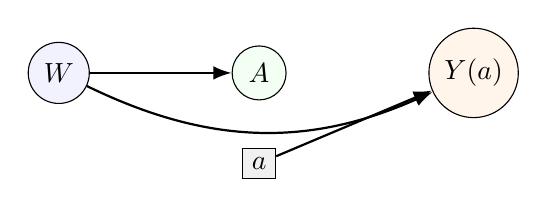
\begin{tikzpicture}[node distance=1.8cm,>=Latex]
  \node[draw, circle, fill=blue!5] (W) {$W$};
  \node[draw, circle, fill=green!5, right=of W] (A) {$A$};
  \node[draw, rectangle, fill=gray!12, below=.6cm of A] (a) {$a$};
  \node[draw, circle, fill=orange!8, right=of A] (Y) {$\Ya{a}$};
  \draw[->, thick] (W) -- (A);
  \draw[->, thick] (W) to[bend right=25] (Y);
  \draw[->, thick] (a) -- (Y);
\end{tikzpicture}
\caption{The fixed node $a$ is not part of random-variable paths, but it defines the intervention world.}
\end{figure}

The path from $A$ to $\Ya{a}$ through $W$ is
\[
A\leftarrow W\to \Ya{a}.
\]
The arrow from $a$ to $\Ya{a}$ does not create a random path from $A$ to $\Ya{a}$ because $a$ is fixed.

\subsection{Colliders and Non-Colliders in SWIGs}

As in DAGs, whether a node is a collider depends on the particular path. A random node $V$ is a collider on a path if the two adjacent arrows on that path both point into $V$:
\[
\cdots \to V \leftarrow \cdots.
\]
Otherwise, $V$ is a non-collider on that path.

A node can be a collider on one path and a non-collider on another. Consider paths between $A$ and $\Ya{a}$ in a SWIG with nodes $W,H,Z$. A node $Z$ may be a collider on
\[
\Ya{a}\leftarrow H\to Z\leftarrow W\to A,
\]
but a non-collider on
\[
\Ya{a}\leftarrow Z\leftarrow A.
\]
The path determines the role.

\subsection{Unconditional d-Separation}

A path d-connects two random nodes unconditionally if it has no closed collider and no conditioned non-collider. With no conditioning set, forks and chains are open, while colliders are closed.

Common open unconditional paths include:
\[
X\to \cdots \to Y,
\qquad
X\leftarrow \cdots \leftarrow Y,
\qquad
X\leftarrow \cdots \leftarrow T\to \cdots \to Y.
\]
The third form is a shared common cause path.

In the SWIG
\[
A\leftarrow W\to \Ya{a},
\]
$A$ and $\Ya{a}$ are not unconditionally d-separated because the fork through $W$ is open. This represents confounding by $W$.

\subsection{Conditional d-Separation}

\begin{definition}[Conditional d-separation in a SWIG]
A path between random nodes is open given a conditioning set $S$ if every non-collider on the path is not in $S$, and every collider on the path is either in $S$ or has a descendant in $S$. Two nodes are d-separated by $S$ if every path between them is blocked by $S$.
\end{definition}

This is the same logic as for DAGs, applied to random nodes in the SWIG. Fixed nodes define interventions but are excluded from conditioning sets.

\subsection{Reading $\Ya{a}\ci A\given W$}

The core use of SWIG d-separation in this chapter is to assess conditional randomization. In the confounding SWIG:

\begin{figure}[H]
\centering
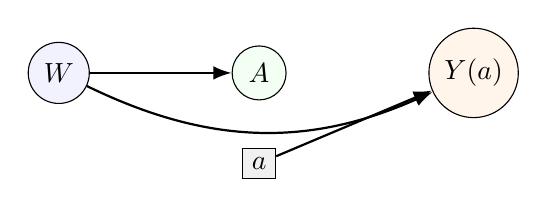
\begin{tikzpicture}[node distance=1.8cm,>=Latex]
  \node[draw, circle, fill=blue!5] (W) {$W$};
  \node[draw, circle, fill=green!5, right=of W] (A) {$A$};
  \node[draw, rectangle, fill=gray!12, below=.6cm of A] (a) {$a$};
  \node[draw, circle, fill=orange!8, right=of A] (Y) {$\Ya{a}$};
  \draw[->, thick] (W) -- (A);
  \draw[->, thick] (W) to[bend right=25] (Y);
  \draw[->, thick] (a) -- (Y);
\end{tikzpicture}
\caption{Conditioning on $W$ blocks the backdoor path from $A$ to $\Ya{a}$.}
\end{figure}

The only random path between $A$ and $\Ya{a}$ is
\[
A\leftarrow W\to \Ya{a}.
\]
This is a fork. Without conditioning, the path is open. Conditioning on $W$ blocks the path. Therefore the SWIG implies
\[
\Ya{a}\ci A\given W.
\]

\begin{keyidea}
In a SWIG, conditional randomization is a d-separation statement between the random treatment node $A$ and the counterfactual outcome node $\Ya{a}$.
\end{keyidea}

If an unmeasured variable $U$ also points to both $A$ and $\Ya{a}$, then the path
\[
A\leftarrow U\to \Ya{a}
\]
remains open after conditioning on measured $W$. In that case the graph does not support $\Ya{a}\ci A\given W$.

\lecture{3.5}{Assumptions for Identifying the ATE}
\label{lec:3-5}

\subsection{Consistency}

To identify the ATE, the observed outcome must be linked to the relevant potential outcome.

\begin{assumptionbox}
\textbf{Consistency.} If a unit is observed with $A=a$, then
\[
Y=\Ya{a}.
\]
For binary $A$,
\[
Y=A\Yone+(1-A)\Yzero.
\]
\end{assumptionbox}

Consistency requires that the treatment versions represented by $A=a$ are well-defined enough that the observed treatment corresponds to the intervention used to define $\Ya{a}$.

\subsection{Conditional Randomization}

The second assumption is conditional randomization, also called conditional exchangeability or conditional ignorability.

\begin{assumptionbox}
\textbf{Conditional randomization.} For $a\in\{0,1\}$,
\[
\Ya{a}\ci A\given W.
\]
Within strata of measured covariates $W$, the observed treatment carries no information about the potential outcome under treatment level $a$.
\end{assumptionbox}

This assumption is usually the hardest to justify in observational studies. It says that $W$ contains enough information to control confounding.

\subsection{Positivity}

Even if treatment is as-if randomized within covariate strata, we must have observed treatment variation within those strata.

\begin{assumptionbox}
\textbf{Positivity.} For each treatment level $a\in\{0,1\}$,
\[
\Prob(A=a\given W=w)>0
\]
for every covariate value $w$ with $\Prob(W=w)>0$.
\end{assumptionbox}

In words, every covariate subgroup in the target population must have some chance of receiving each treatment level. If no mildly ill patients ever receive a risky experimental treatment, then the observed data contain no direct information about outcomes under that treatment for mildly ill patients.

\subsection{Why Positivity Is Partly Empirically Checkable}

Unlike exchangeability, positivity is stated in terms of the observed data distribution. It involves $\Prob(A=a\given W=w)$, not counterfactual outcomes. Therefore it can be partly checked.

For discrete $W$, one can inspect whether each covariate stratum contains both treated and untreated observations. For continuous or high-dimensional $W$, exact strata may be sparse, so analysts examine estimated propensity scores
\[
g_a(W)=\Prob(A=a\given W)
\]
and check whether they are close to zero.

Empirical checks are not perfect. A finite sample may fail to show a treatment level in a subgroup even if the population probability is positive. Conversely, a few observations in a subgroup do not guarantee enough information for stable estimation. Still, positivity has observable implications.

\subsection{Why Positivity Matters for Observed Conditional Means}

The G-computation formula will involve terms such as
\[
\E(Y\given A=a,W=w).
\]
This conditional mean is defined from the observed data distribution only when $\Prob(A=a,W=w)>0$. Since
\[
\Prob(A=a,W=w)=\Prob(A=a\given W=w)\Prob(W=w),
\]
if $\Prob(W=w)>0$ but $\Prob(A=a\given W=w)=0$, then the subgroup $(A=a,W=w)$ does not exist in the observed population. The conditional mean cannot be learned from observed outcomes.

\begin{keyidea}
Exchangeability says treated and untreated people are comparable within $W$ strata. Positivity says both treated and untreated people actually exist within those strata.
\end{keyidea}

\lecture{3.6}{G-Computation Identification Formula}
\label{lec:3-6}

\subsection{Derivation of $\E\{\Ya{a}\}$}

Assume consistency, conditional randomization, and positivity. For a discrete covariate vector $W$, begin with the counterfactual mean:
\[
\E\{\Ya{a}\}.
\]
Apply the tower rule by averaging over covariate strata:
\[
\E\{\Ya{a}\}
=
\sum_w \E\{\Ya{a}\given W=w\}\Prob(W=w).
\]
Use conditional randomization, $\Ya{a}\ci A\given W$, to add the event $A=a$ inside the conditional expectation:
\[
\E\{\Ya{a}\given W=w\}
=
\E\{\Ya{a}\given A=a,W=w\}.
\]
Then use consistency. Among units with $A=a$, the observed outcome equals $\Ya{a}$:
\[
\E\{\Ya{a}\given A=a,W=w\}
=
\E(Y\given A=a,W=w).
\]
Substituting gives
\[
\E\{\Ya{a}\}
=
\sum_w \E(Y\given A=a,W=w)\Prob(W=w).
\]
Equivalently,
\[
\E\{\Ya{a}\}
=
\E\{\E(Y\given A=a,W)\}.
\]

\begin{identificationbox}
\textbf{G-computation identification formula.} Under consistency, conditional randomization, and positivity,
\[
\E\{\Ya{a}\}
=
\E\{\E(Y\given A=a,W)\}.
\]
Therefore
\[
\ATE
=
\E\{\E(Y\given A=1,W)-\E(Y\given A=0,W)\}.
\]
\end{identificationbox}

\subsection{Role of the Tower Rule}

The tower rule is the first step:
\[
\E\{\Ya{a}\}
=\sum_w \E\{\Ya{a}\given W=w\}\Prob(W=w).
\]
It says that the population mean counterfactual outcome is a weighted average of covariate-specific counterfactual means. The weights are the covariate distribution in the whole target population.

\subsection{Role of Conditional Randomization}

Conditional randomization justifies replacing the counterfactual mean in the whole $W=w$ stratum with the counterfactual mean among the observed treatment subgroup:
\[
\E\{\Ya{a}\given W=w\}
=
\E\{\Ya{a}\given A=a,W=w\}.
\]
In words, within the stratum $W=w$, people who actually received $A=a$ are representative of everyone in that stratum with respect to $\Ya{a}$.

\subsection{Role of Consistency}

Consistency changes the counterfactual outcome into an observed outcome among those who received $A=a$:
\[
\E\{\Ya{a}\given A=a,W=w\}
=
\E(Y\given A=a,W=w).
\]
This is where the expression becomes fully observed-data based.

\subsection{Interpretation as Standardization}

The formula
\[
\sum_w \E(Y\given A=a,W=w)\Prob(W=w)
\]
standardizes treatment-specific outcome means to the covariate distribution of the whole population.

For each $w$:
\begin{enumerate}
  \item compute the average observed outcome among people with $A=a$ and $W=w$;
  \item weight that subgroup mean by the population prevalence $\Prob(W=w)$;
  \item sum over all covariate strata.
\end{enumerate}

\subsection{G-Computation Intuition}

Within each $W=w$ stratum, conditional randomization makes the observed comparison between $A=1$ and $A=0$ fair. The subgroup-specific causal contrast is
\[
\E(Y\given A=1,W=w)-\E(Y\given A=0,W=w).
\]
The population ATE averages these fair subgroup comparisons using the target population distribution of $W$:
\[
\ATE
=
\sum_w
\left\{
\E(Y\given A=1,W=w)-\E(Y\given A=0,W=w)
\right\}\Prob(W=w).
\]

\subsection{Worked Discrete Example}

Let $Y$ indicate death due to cancer, let $A=1$ denote a risky treatment and
$A=0$ denote standard treatment, and let $W=1$ denote severe disease. Consider a
population of 320 people with the following observed counts:
\[
\begin{array}{c|cc|cc}
& \multicolumn{2}{c|}{W=0} & \multicolumn{2}{c}{W=1}\\
& A=0 & A=1 & A=0 & A=1\\
\hline
Y=1 & 60 & 10 & 30 & 60\\
Y=0 & 60 & 30 & 10 & 60
\end{array}
\]
Each covariate stratum contains people at both treatment levels, so positivity holds:
\[
\Prob(A=a\given W=w)>0
\qquad\text{for all }a\in\{0,1\},\;w\in\{0,1\}.
\]
Suppose conditional randomization and consistency are also valid. Then the observed
conditional outcome means identify the stratum-specific counterfactual risks.

For the risky treatment,
\[
\E(Y\given A=1,W=0)=\frac{10}{10+30}=0.25,
\]
and
\[
\E(Y\given A=1,W=1)=\frac{60}{60+60}=0.50.
\]
Because the population has 160 people with $W=0$ and 160 people with $W=1$,
\[
\Prob(W=0)=\Prob(W=1)=0.50.
\]
Therefore
\[
\E\{\Yone\}
=0.25(0.50)+0.50(0.50)=0.375.
\]
For standard treatment,
\[
\E(Y\given A=0,W=0)=\frac{60}{60+60}=0.50,
\qquad
\E(Y\given A=0,W=1)=\frac{30}{30+10}=0.75,
\]
so
\[
\E\{\Yzero\}
=0.50(0.50)+0.75(0.50)=0.625.
\]
The identified ATE on the risk-difference scale is
\[
\E\{\Yone\}-\E\{\Yzero\}=0.375-0.625=-0.25.
\]
Because $Y=1$ means death, this negative value means the risky treatment lowers
the death risk by 25 percentage points in this population under the stated
assumptions.

\subsection{Why Naive Mean Differences Are Unfair}

The naive observed mean difference is
\[
\E(Y\given A=1)-\E(Y\given A=0).
\]
By the tower rule,
\[
\E(Y\given A=1)
=
\sum_w \E(Y\given A=1,W=w)\Prob(W=w\given A=1),
\]
and
\[
\E(Y\given A=0)
=
\sum_w \E(Y\given A=0,W=w)\Prob(W=w\given A=0).
\]
Thus the treated mean is averaged over the covariate distribution among treated people, while the untreated mean is averaged over the covariate distribution among untreated people. If treatment groups have different covariate distributions, the comparison mixes treatment differences with covariate-composition differences.

In the cancer example above, the risky treatment group has more severe patients:
\[
\Prob(W=1\given A=1)=\frac{120}{160}=0.75,
\qquad
\Prob(W=1\given A=0)=\frac{40}{160}=0.25.
\]
The naive risks are
\[
\E(Y\given A=1)=\frac{10+60}{160}=0.4375,
\qquad
\E(Y\given A=0)=\frac{60+30}{160}=0.5625,
\]
so the naive difference is $-0.125$, only half as large in magnitude as the
standardized contrast $-0.25$. The naive comparison is unfair to the risky
treatment because it averages the risky-treatment outcomes over a much sicker
covariate distribution.

\begin{keyidea}
G-computation keeps the comparison fair by using the same covariate distribution, $\Prob(W=w)$, for both treatment levels.
\end{keyidea}

\lecture{3.7}{Other Causal Estimands}
\label{lec:3-7}

\subsection{Conditional Average Treatment Effect}

Suppose $W=(X,Z)$, where $X$ defines a subgroup of scientific interest and $Z$ contains additional covariates needed for confounding control. The conditional average treatment effect as a function of $X$ is
\[
\CATE(x)=\E(\Yone-\Yzero\given X=x).
\]
Under the same consistency, conditional randomization, and positivity assumptions, with randomization conditional on $(X,Z)$, the G-computation formula becomes
\[
\begin{aligned}
\CATE(x)
&=
\sum_z
\Big[
\E(Y\given A=1,X=x,Z=z)
-
\E(Y\given A=0,X=x,Z=z)
\Big] \\
&\qquad {}\times \Prob(Z=z\given X=x).
\end{aligned}
\]

The logic is the same as for the ATE. Within each $(X=x,Z=z)$ stratum, the treatment comparison is fair. Then we average over the distribution of $Z$ among people with $X=x$.

\subsection{Effect Heterogeneity}

\begin{definition}[Effect heterogeneity]
There is effect heterogeneity by $X$ on the additive scale if
\[
\CATE(x)=\E(\Yone-\Yzero\given X=x)
\]
varies with $x$.
\end{definition}

On a ratio scale, one might define
\[
\frac{\E(\Yone\given X=x)}{\E(\Yzero\given X=x)}
\]
and say there is heterogeneity if this ratio varies with $x$. Effect heterogeneity is therefore scale-specific.

\subsection{Average Treatment Effect among the Treated}

Sometimes the causal effect in the whole population is not the most relevant target. If an intervention can only be applied to people who would naturally seek it, the effect among those actually treated may be more meaningful.

\begin{definition}[Average treatment effect among the treated]
For binary treatment,
\[
\ATT=\E(\Yone-\Yzero\given A=1).
\]
\end{definition}

Under standard assumptions,
\[
\ATT
=
\sum_w
\left\{
\E(Y\given A=1,W=w)-\E(Y\given A=0,W=w)
\right\}
\Prob(W=w\given A=1).
\]
The weighting distribution is now the covariate distribution among treated people, not the full population distribution.

\subsection{Average Treatment Effect among Controls}

\begin{definition}[Average treatment effect among controls]
For binary treatment,
\[
\ATC=\E(\Yone-\Yzero\given A=0).
\]
\end{definition}

The identified G-computation expression is
\[
\ATC
=
\sum_w
\left\{
\E(Y\given A=1,W=w)-\E(Y\given A=0,W=w)
\right\}
\Prob(W=w\given A=0).
\]
This estimand answers what the average effect would be among people who were not treated in the observed world.

\subsection{Relationship among ATE, ATT, and ATC}

The ATE is a weighted combination of ATT and ATC. Apply the tower rule to $\Yone-\Yzero$ conditioning on $A$:
\[
\ATE
=
\E(\Yone-\Yzero)
=
\E\{\E(\Yone-\Yzero\given A)\}.
\]
Since $A$ is binary,
\[
\ATE
=
\E(\Yone-\Yzero\given A=1)\Prob(A=1)
+
\E(\Yone-\Yzero\given A=0)\Prob(A=0).
\]
Therefore
\[
\ATE=\ATT\Prob(A=1)+\ATC\Prob(A=0).
\]

\begin{keyidea}
ATE, ATT, and ATC differ in the population over which subgroup-specific effects are averaged.
\end{keyidea}

\subsection{Causal Effect Interaction}

With two binary treatments $A_1$ and $A_2$, potential outcomes are written
\[
Y(a_1,a_2).
\]
There is additive interaction if the joint effect differs from the sum of the separate effects:
\[
\E\{Y(1,1)-Y(0,0)\}
\ne
\E\{Y(1,0)-Y(0,0)\}
+
\E\{Y(0,1)-Y(0,0)\}.
\]
For example, chemotherapy and radiation may have a joint effect that is larger or smaller than the sum of their individual effects.

On a ratio scale, interaction is defined differently:
\[
\frac{\E\{Y(1,1)\}}{\E\{Y(0,0)\}}
\ne
\frac{\E\{Y(1,0)\}}{\E\{Y(0,0)\}}
\times
\frac{\E\{Y(0,1)\}}{\E\{Y(0,0)\}}.
\]
The choice of additive or multiplicative scale should be driven by the scientific question.

\lecture{3.8}{IPTW Identification Formula}
\label{lec:3-8}

\subsection{Inverse Probability Weighting}

G-computation identifies counterfactual means by standardizing conditional outcome means. Inverse probability of treatment weighting, or IPTW, identifies the same counterfactual means by reweighting observed outcomes.

\begin{definition}[IPTW identification formula]
Under consistency, conditional randomization, and positivity,
\[
\E\{\Ya{a}\}
=
\E\left\{
\frac{\ind(A=a)Y}{\Prob(A=a\given W)}
\right\}.
\]
\end{definition}

Only people who actually received $A=a$ contribute to the numerator, because $\ind(A=a)=0$ for everyone else. Those who did receive $A=a$ are weighted by the inverse of their probability of receiving that treatment.

\subsection{Propensity Score}

\begin{definition}[Propensity score]
For binary treatment, the propensity score is
\[
g(W)=\Prob(A=1\given W).
\]
More generally, write
\[
g_a(W)=\Prob(A=a\given W).
\]
\end{definition}

The IPTW formula for treatment level $a$ uses $g_a(W)$:
\[
\E\{\Ya{a}\}
=
\E\left\{\frac{\ind(A=a)Y}{g_a(W)}\right\}.
\]

\subsection{IPTW Derivation}

We derive the observed-data equality. Start with
\[
\E\left\{\frac{\ind(A=a)Y}{g_a(W)}\right\}.
\]
Apply the tower rule conditioning on $A$ and $W$:
\[
=
\E\left[
\E\left\{
\frac{\ind(A=a)Y}{g_a(W)}
\given A,W
\right\}
\right].
\]
Inside the conditional expectation, $\ind(A=a)$ and $g_a(W)$ are known:
\[
=
\E\left[
\frac{\ind(A=a)}{g_a(W)}
\E(Y\given A,W)
\right].
\]
Because the indicator is zero unless $A=a$,
\[
=
\E\left[
\frac{\ind(A=a)}{g_a(W)}
\E(Y\given A=a,W)
\right].
\]
Apply the tower rule again, now conditioning on $W$:
\[
=
\E\left[
\E\left\{
\frac{\ind(A=a)}{g_a(W)}
\E(Y\given A=a,W)
\given W
\right\}
\right].
\]
Given $W$, the outcome regression term and denominator are fixed:
\[
=
\E\left[
\frac{\E(Y\given A=a,W)}{g_a(W)}
\E\{\ind(A=a)\given W\}
\right].
\]
But
\[
\E\{\ind(A=a)\given W\}=\Prob(A=a\given W)=g_a(W).
\]
Thus
\[
=
\E\left[
\frac{\E(Y\given A=a,W)}{g_a(W)}g_a(W)
\right]
=
\E\{\E(Y\given A=a,W)\}.
\]
By the G-computation identification formula, this equals $\E\{\Ya{a}\}$.

\begin{identificationbox}
\[
\E\{\Ya{a}\}
=
\E\{\E(Y\given A=a,W)\}
=
\E\left\{
\frac{\ind(A=a)Y}{\Prob(A=a\given W)}
\right\}.
\]
The first equality is G-computation. The second is IPTW. They identify the same counterfactual mean under the same assumptions.
\end{identificationbox}

\subsection{Pseudo-Population Intuition}

Suppose a treated patient had only a $5\%$ chance of receiving treatment given $W$. Then treated patients with that covariate pattern are rare. One such treated patient represents many similar people who, under the observed treatment mechanism, usually did not receive treatment. The IPTW weight is
\[
\frac{1}{0.05}=20.
\]
If another treated patient had a $75\%$ chance of receiving treatment, the weight is
\[
\frac{1}{0.75}\approx 1.33.
\]
IPTW upweights observations who received a treatment that was unlikely for their covariate profile and downweights observations who received a treatment that was common.

\subsection{Stabilizing Representativeness}

The weighted treated group is designed to represent the whole target population with respect to $W$. In expectation,
\[
\E\left\{\frac{\ind(A=a)}{g_a(W)}\given W\right\}
=
\frac{1}{g_a(W)}\Prob(A=a\given W)
=1.
\]
Thus each covariate stratum contributes according to its population prevalence after weighting.

\subsection{Positivity and Extreme Weights}

The formula requires $g_a(W)>0$. If $g_a(W)=0$, the weight is undefined and no observed unit with that covariate value received treatment $a$.

Even when $g_a(W)$ is positive but very small, weights can be very large. Large weights make estimation unstable because a few observations can dominate the weighted mean. This is a practical manifestation of near-positivity violations.

\begin{keyidea}
IPTW creates a weighted pseudo-population in which treatment is no longer associated with measured covariates. Positivity is required so every needed type of person can appear under every treatment level.
\end{keyidea}

\lecture{3.9}{Equivalence and Extensions}
\label{lec:3-9}

\subsection{Equivalence of G-Computation and IPTW Identification}

G-computation and IPTW look different, but they are algebraically equivalent as identification formulas. For $a=1$,
\[
\E\left\{\frac{\ind(A=1)Y}{\Prob(A=1\given W)}\right\}
=
\E\{\E(Y\given A=1,W)\}.
\]
The derivation follows from repeated use of the tower rule:
\[
\E\left\{\frac{\ind(A=1)Y}{g_1(W)}\right\}
=
\E\left[
\E\left\{
\frac{\ind(A=1)Y}{g_1(W)}
\given A,W
\right\}
\right]
\]
\[
=
\E\left[
\frac{\ind(A=1)}{g_1(W)}
\E(Y\given A,W)
\right]
=
\E\left[
\frac{\ind(A=1)}{g_1(W)}
\E(Y\given A=1,W)
\right]
\]
\[
=
\E\left[
\E\left\{
\frac{\ind(A=1)}{g_1(W)}
\E(Y\given A=1,W)
\given W
\right\}
\right]
\]
\[
=
\E\left[
\frac{\E(Y\given A=1,W)}{g_1(W)}
\E\{\ind(A=1)\given W\}
\right]
=
\E\{\E(Y\given A=1,W)\}.
\]

\subsection{Conditioning on the Propensity Score}

The propensity score is a balancing score. Under conditional randomization and positivity,
\[
(\Yone,\Yzero)\ci A\given g(W),
\]
where $g(W)=\Prob(A=1\given W)$.

The intuition is that within groups of people who have the same probability of treatment, the covariate information relevant to treatment assignment has been balanced sufficiently for exchangeability.

The ATE can therefore also be identified by
\[
\ATE
=
\E\left[
\E(Y\given A=1,g(W))
-
\E(Y\given A=0,g(W))
\right],
\]
where the outer expectation is over the population distribution of $g(W)$.

\subsection{Collider Bias}

Colliders are a major reason that "adjust for everything" is not a valid causal strategy. Consider a picnic example:
\begin{itemize}
  \item $A=1$ means chicken salad, $A=0$ means egg salad;
  \item $Y=1$ means a person already has influenza;
  \item $C=1$ means fever after the picnic.
\end{itemize}
Suppose egg salad is tainted and causes fever, influenza also causes fever, and the sandwich does not cause influenza. Then $C$ is a collider:
\[
A\to C\leftarrow Y.
\]

\begin{figure}[H]
\centering
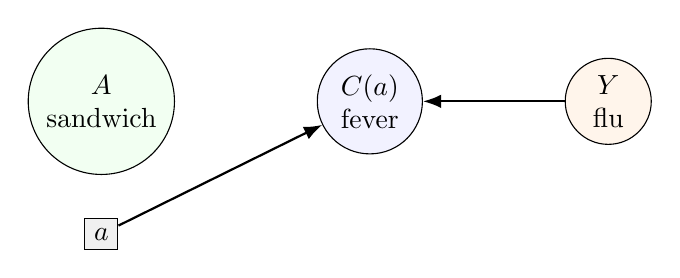
\begin{tikzpicture}[node distance=1.8cm,>=Latex]
  \node[draw, circle, fill=green!5] (A) {$A$\\sandwich};
  \node[draw, rectangle, fill=gray!12, below=.55cm of A] (a) {$a$};
  \node[draw, circle, fill=blue!5, right=of A] (C) {$C(a)$\\fever};
  \node[draw, circle, fill=orange!8, right=of C] (Y) {$Y$\\flu};
  \draw[->, thick] (a) -- (C);
  \draw[->, thick] (Y) -- (C);
\end{tikzpicture}
\caption{Conditioning on fever opens a path between sandwich type and influenza.}
\end{figure}

Since $Y$ is not downstream of $A$, there is no causal effect of sandwich on influenza. Unconditionally, $A$ and $Y$ may be independent. But conditioning on fever induces dependence: among people with fever, knowing the person ate chicken salad makes influenza more likely because chicken salad did not explain the fever.

\begin{keyidea}
Conditioning can create bias when the conditioned variable is a collider or a descendant of a collider.
\end{keyidea}

\subsection{Causal Effect among Compliers}

In some randomized studies, assignment $Z$ is randomized but treatment actually taken $A$ is not fully controlled. Some participants comply with assignment, while others do not. A common causal target is the effect among compliers:
\[
\E\{Y(1)-Y(0)\given A(1)=1,A(0)=0\},
\]
where $A(z)$ is the treatment that would be taken under assignment $Z=z$.

This estimand is not an ordinary ATE in the full population. It is an effect in a latent subgroup defined by joint potential treatment behaviors under two assignment levels.

\subsection{Principal Stratification}

Principal stratification defines subgroups using potential values of an intermediate variable. For example, in a vaccine study, one might ask for the effect of vaccination on growth among children who would have been infected without vaccination:
\[
\E\{G(1)-G(0)\given I(0)=1\}.
\]
Here $I(0)$ is infection status under no vaccination and $G(a)$ is growth under vaccination level $a$.

Principal strata can be scientifically appealing, but they often involve cross-world or partially latent quantities. Identification typically requires assumptions beyond standard exchangeability and positivity.

\subsection{Transition from Identification to Estimation}

This chapter has produced observed-data parameters for causal quantities. For example,
\[
\E\{\Ya{a}\}
=
\E\{\E(Y\given A=a,W)\}
\]
and
\[
\E\{\Ya{a}\}
=
\E\left\{
\frac{\ind(A=a)Y}{\Prob(A=a\given W)}
\right\}.
\]
These formulas do not yet tell us how to estimate the quantities in finite samples. They tell us what must be estimated: outcome regressions, propensity scores, covariate distributions, and expectations.

\begin{estimationbox}
The next step is estimation. Once identification has converted counterfactual parameters into observed-data parameters, we can construct estimators such as plug-in G-computation estimators, IPTW estimators, and later doubly robust estimators.
\end{estimationbox}


\chapterheading{4}{Basic Estimation of the Average Treatment Effect}
\lecture{4.1}{From Identification to Estimation}
\label{lec:4-1}

\subsection{Observed Data Structure: $O=(W,A,Y)$}

In the previous chapter, the average treatment effect was identified under consistency,
conditional randomization, and positivity. Identification gave formulas involving only
the observed-data distribution. Estimation begins after that step: we now have a
sample and must turn the identified statistical parameter into a numerical estimate.

Throughout this chapter the observed data are
\[
O_i=(W_i,A_i,Y_i), \qquad i=1,\ldots,n,
\]
where the observations are assumed to be independent and identically distributed:
\[
O_1,\ldots,O_n \iid P.
\]
Here $W$ is a vector of pre-treatment covariates, $A\in\{0,1\}$ is treatment, and
$Y$ is the outcome. The phrase ``pre-treatment'' is important. Variables affected by
treatment are not ordinary confounders for the effect of $A$ on $Y$ in a point-treatment
analysis, because adjusting for them can block part of the causal effect or create
collider bias.

\begin{assumptionbox}
The estimators in this chapter are estimators of causal effects only when the
identification assumptions from Chapter 3 are scientifically credible:
\[
Y(a)=Y \text{ if } A=a,\qquad
\Ya{a}\ci A\given W,\qquad
\Prob(A=a\given W=w)>0
\]
for all treatment levels $a$ and all covariate values $w$ in the target population.
Without these assumptions, the same formulas estimate well-defined statistical
parameters, but those parameters need not equal counterfactual means.
\end{assumptionbox}

\subsection{Outcome Regression $\Qbar(a,w)$}

\begin{definition}[Outcome regression]
The outcome regression is the conditional mean of the observed outcome given
treatment and covariates:
\[
\Qbar(a,w)=\E(Y\given A=a,W=w).
\]
\end{definition}

This function answers an observed-data question: among individuals who actually
received treatment level $a$ and had covariates $W=w$, what was the mean outcome?
Under the identification assumptions, this observed subgroup mean can be used as a
building block for the mean counterfactual outcome under treatment level $a$.

For a binary outcome, $\Qbar(a,w)$ is a conditional risk:
\[
\Qbar(a,w)=\Prob(Y=1\given A=a,W=w).
\]
For a continuous outcome, it is a conditional average. For an ordinal or count outcome,
it is still a conditional mean, although the mean may not fully summarize the whole
conditional distribution.

\subsection{Propensity Score $g_a(w)$}

\begin{definition}[Propensity score]
For a binary treatment, the treatment-specific propensity score is
\[
g_a(w)=\Prob(A=a\given W=w).
\]
The usual propensity score is $g_1(w)=\Prob(A=1\given W=w)$, and
$g_0(w)=1-g_1(w)$.
\end{definition}

The propensity score describes how treatment is assigned in the observed population.
It is not a causal effect. Instead, it measures the treatment probability among people
with covariate value $w$. In inverse probability weighting, individuals who received a
treatment level that was unlikely for their covariates receive larger weights. These
weights compensate for the unequal representation of covariate strata across treatment
groups.

\subsection{Plug-In Estimation}

The g-computation identification formula for the counterfactual mean is
\[
\psi(a)=\E\{\Ya{a}\}=\E\{\Qbar(a,W)\}.
\]
This formula contains two features of the observed-data distribution:
the conditional mean function $\Qbar(a,w)$ and the marginal distribution of $W$.
A plug-in estimator replaces each unknown population quantity by an estimate from
the data.

\begin{definition}[Plug-in estimator]
A plug-in estimator is obtained by writing the target parameter as a function of the
observed-data distribution and then substituting empirical or model-based estimates
for the unknown components of that distribution.
\end{definition}

If $\Qbar_n(a,w)$ estimates $\Qbar(a,w)$, the natural g-computation plug-in estimator is
\[
\psi_n^{\mathrm{gcomp}}(a)
=
\frac{1}{n}\sum_{i=1}^n \Qbar_n(a,W_i).
\]
This expression averages predicted outcomes under treatment level $a$ over the
observed covariate distribution. The observed covariates $W_1,\ldots,W_n$ are used
as an empirical approximation to the target population distribution of $W$.

\begin{figure}[H]
\centering
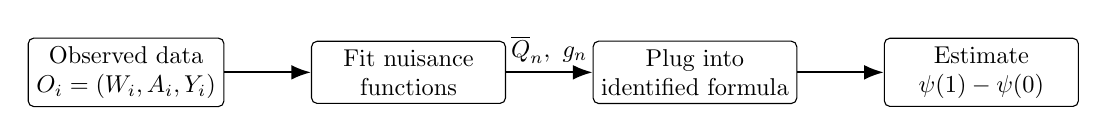
\begin{tikzpicture}[
  scale=.88,
  transform shape,
  node distance=1.25cm,
  box/.style={draw, rounded corners=2pt, minimum width=2.8cm, minimum height=.85cm},
  arr/.style={-{Latex[length=2.5mm]}, thick}
]
\node[box] (data) {Observed data\\ $O_i=(W_i,A_i,Y_i)$};
\node[box, right=of data] (fit) {Fit nuisance\\ functions};
\node[box, right=of fit] (plugin) {Plug into\\ identified formula};
\node[box, right=of plugin] (ate) {Estimate\\ $\psi(1)-\psi(0)$};
\draw[arr] (data) -- (fit);
\draw[arr] (fit) -- node[above] {$\Qbar_n,\ g_n$} (plugin);
\draw[arr] (plugin) -- (ate);
\end{tikzpicture}
\caption{Estimation turns the identified observed-data parameter into a sample quantity.}
\label{fig:ch4-estimation-flow}
\end{figure}

\subsection{Estimating Counterfactual Means}

There are two basic plug-in strategies emphasized in this chapter.

The first uses the outcome regression:
\[
\psi_n^{\mathrm{gcomp}}(a)=\frac{1}{n}\sum_{i=1}^n \Qbar_n(a,W_i).
\]
For each observed individual, we keep $W_i$ fixed and replace the observed treatment
by the hypothetical treatment value $a$ inside the fitted outcome regression. The
resulting predicted values are then averaged.

The second uses inverse probability weighting. If $g_{n,a}(w)$ estimates
$g_a(w)=\Prob(A=a\given W=w)$, then
\[
\psi_n^{\IPTW}(a)
=
\frac{1}{n}\sum_{i=1}^n
\frac{\ind(A_i=a)}{g_{n,a}(W_i)}Y_i.
\]
Only people who actually received treatment level $a$ contribute to the estimate of
$\E\{\Ya{a}\}$, but their outcomes are weighted by the inverse of their estimated
probability of receiving that treatment.

\begin{keyidea}
G-computation estimates counterfactual means by predicting everyone's outcome under
each treatment level. IPTW estimates counterfactual means by reweighting the people
who actually received each treatment level so that, after weighting, they represent the
full target population.
\end{keyidea}

\subsection{Estimating the ATE}

The average treatment effect is
\[
\ATE=\E\{\Yone\}-\E\{\Yzero\}=\psi(1)-\psi(0).
\]
The corresponding g-computation estimator is
\[
\widehat{\ATE}_{\mathrm{gcomp}}
=
\frac{1}{n}\sum_{i=1}^n
\left\{
\Qbar_n(1,W_i)-\Qbar_n(0,W_i)
\right\}.
\]
The corresponding IPTW estimator is
\[
\widehat{\ATE}_{\IPTW}
=
\frac{1}{n}\sum_{i=1}^n
\left\{
\frac{\ind(A_i=1)}{g_{n,1}(W_i)}Y_i
-
\frac{\ind(A_i=0)}{g_{n,0}(W_i)}Y_i
\right\}.
\]

\begin{estimationbox}
Basic estimation workflow for the ATE:
\begin{enumerate}
\item Choose whether to estimate the counterfactual means using the outcome
regression, the propensity score, or both in a later doubly robust method.
\item Estimate the nuisance function required by the chosen method.
\item Construct $\psi_n(1)$ and $\psi_n(0)$ using the identified formula.
\item Report $\widehat{\ATE}=\psi_n(1)-\psi_n(0)$.
\item Quantify uncertainty using an appropriate variance estimator or resampling
method such as the bootstrap.
\end{enumerate}
\end{estimationbox}

\lecture{4.2}{G-Computation with Discrete Data}
\label{lec:4-2}

\subsection{Empirical Mean Outcome Regression}

When $W$ takes only a small number of possible values, the most direct estimator of
the outcome regression is the sample mean within each $(A,W)$ subgroup. For a fixed
treatment value $a$ and covariate value $w$, define
\[
n_{aw}=\sum_{i=1}^n \ind(A_i=a,W_i=w).
\]
If $n_{aw}>0$, the empirical outcome regression is
\[
\Qbar_n(a,w)
=
\frac{\sum_{i=1}^n Y_i\ind(A_i=a,W_i=w)}
       {\sum_{i=1}^n \ind(A_i=a,W_i=w)}.
\]
This is simply the average observed outcome among people with treatment $A=a$ and
covariates $W=w$.

For example, if $W$ is a binary age indicator, then $\Qbar_n(1,0)$ is the sample mean
outcome among younger treated individuals, while $\Qbar_n(0,1)$ is the sample mean
outcome among older untreated individuals.

\begin{keyidea}
With low-dimensional discrete covariates, empirical g-computation is ordinary
stratification. Estimate the mean outcome in each treatment-covariate stratum, then
average those stratum means using the covariate distribution of the target population.
\end{keyidea}

\subsection{Saturated Regression Models}

A saturated model has enough parameters to reproduce every subgroup mean. With
binary $A$ and binary $W$, there are four treatment-covariate subgroups. A saturated
linear mean model is
\[
\E(Y\given A=a,W=w)=\beta_0+\beta_1 a+\beta_2 w+\beta_3 aw.
\]
The fitted means implied by this model are
\[
\begin{array}{c|cc}
& A=0 & A=1\\
\hline
W=0 & \beta_0 & \beta_0+\beta_1\\
W=1 & \beta_0+\beta_2 & \beta_0+\beta_1+\beta_2+\beta_3 .
\end{array}
\]
Because there are four parameters and four subgroup means, the model can exactly
match the empirical subgroup averages whenever each subgroup is observed. The
interaction term $aw$ is what makes the model saturated. Without it, the model would
force the treatment contrast to be the same at both levels of $W$ on the additive
scale.

\begin{remark}
The word ``saturated'' is about flexibility relative to the chosen covariate
description. If $W$ has many categories or multiple components, a truly saturated
model may require many main effects and interactions.
\end{remark}

\subsection{Estimating $\Prob(W=w)$}

The g-computation parameter also requires the marginal distribution of $W$:
\[
\psi(a)=\sum_w \Qbar(a,w)\Prob(W=w).
\]
For discrete $W$, the empirical estimator is the sample proportion
\[
P_n(W=w)
=
\frac{1}{n}\sum_{i=1}^n \ind(W_i=w).
\]
This is the fraction of the sample in covariate stratum $w$. It estimates the covariate
distribution in the target population represented by the sample.

\subsection{Computing $\E\{\Yone\}$}

The g-computation estimator of $\E\{\Yone\}$ is obtained by setting $a=1$:
\[
\psi_n(1)
=
\sum_w \Qbar_n(1,w)P_n(W=w).
\]
For binary $W$, this becomes
\[
\psi_n(1)
=
\Qbar_n(1,0)P_n(W=0)+\Qbar_n(1,1)P_n(W=1).
\]
The first term is the estimated treated mean outcome among people with $W=0$,
weighted by how common $W=0$ is in the full sample. The second term is the analogous
quantity for $W=1$.

\subsection{Computing $\E\{\Yzero\}$}

Similarly,
\[
\psi_n(0)
=
\sum_w \Qbar_n(0,w)P_n(W=w),
\]
and for binary $W$,
\[
\psi_n(0)
=
\Qbar_n(0,0)P_n(W=0)+\Qbar_n(0,1)P_n(W=1).
\]
This estimates the mean outcome that would have been observed if everyone in the
target population had received treatment level $0$.

\subsection{Computing the ATE}

The estimated average treatment effect is the difference between the two estimated
counterfactual means:
\[
\widehat{\ATE}_{\mathrm{gcomp}}
=
\psi_n(1)-\psi_n(0).
\]
Equivalently,
\[
\widehat{\ATE}_{\mathrm{gcomp}}
=
\sum_w
\left\{
\Qbar_n(1,w)-\Qbar_n(0,w)
\right\}P_n(W=w).
\]
This expression shows that empirical g-computation is a weighted average of
stratum-specific treatment contrasts. The weights are not the covariate distributions
inside the treated and untreated groups separately. They are the covariate distribution
of the full target sample.

\subsection{Equivalent Individual-Level Form}

Because $P_n(W=w)$ is the fraction of individuals whose covariates equal $w$, the
same estimator can be written as
\[
\psi_n(a)
=
\frac{1}{n}\sum_{i=1}^n \Qbar_n(a,W_i).
\]
To see this, start from the subgroup formula:
\[
\sum_w \Qbar_n(a,w)P_n(W=w)
=
\sum_w \Qbar_n(a,w)
\left\{
\frac{1}{n}\sum_{i=1}^n \ind(W_i=w)
\right\}.
\]
Move the finite sum over observations outside:
\[
=
\frac{1}{n}\sum_{i=1}^n
\sum_w \Qbar_n(a,w)\ind(W_i=w).
\]
For each individual $i$, exactly one value of $w$ equals $W_i$, so the inner sum is
$\Qbar_n(a,W_i)$. Therefore,
\[
\sum_w \Qbar_n(a,w)P_n(W=w)
=
\frac{1}{n}\sum_{i=1}^n \Qbar_n(a,W_i).
\]

\subsection{By-Hand Example}

Suppose $W$ is binary and the sample summaries are as follows:
\[
\begin{array}{c|cc|c}
W & \Qbar_n(0,W) & \Qbar_n(1,W) & P_n(W)\\
\hline
0 & 2.680 & 2.875 & 0.370\\
1 & 2.222 & 2.327 & 0.630
\end{array}
\]
Then
\[
\psi_n(1)=2.875(0.370)+2.327(0.630)=2.530,
\]
and
\[
\psi_n(0)=2.680(0.370)+2.222(0.630)=2.392.
\]
Thus
\[
\widehat{\ATE}_{\mathrm{gcomp}}=2.530-2.392=0.138.
\]
The interpretation is that, after standardizing the treated and untreated subgroup
means to the same covariate distribution, the estimated mean outcome is about 0.138 units
higher under treatment than under no treatment.

\begin{estimationbox}
By-hand empirical g-computation:
\begin{enumerate}
\item List all observed covariate strata $w$.
\item Compute $\Qbar_n(1,w)$ and $\Qbar_n(0,w)$ within each stratum.
\item Compute $P_n(W=w)$ for each stratum.
\item Form $\psi_n(1)=\sum_w \Qbar_n(1,w)P_n(W=w)$.
\item Form $\psi_n(0)=\sum_w \Qbar_n(0,w)P_n(W=w)$.
\item Subtract to obtain $\widehat{\ATE}_{\mathrm{gcomp}}$.
\end{enumerate}
\end{estimationbox}

\lecture{4.3}{G-Computation Using Regression Models}
\label{lec:4-3}

\subsection{Prediction-Based Implementation}

Empirical g-computation by hand is transparent, but it becomes cumbersome when $W$
has many components. Regression provides a systematic way to estimate
$\Qbar(a,w)=\E(Y\given A=a,W=w)$ and then evaluate the fitted regression under
counterfactual treatment values.

The generic regression-based g-computation estimator is
\[
\psi_n(a)=\frac{1}{n}\sum_{i=1}^n \Qbar_n(a,W_i),
\]
where $\Qbar_n$ is a fitted outcome regression. The estimated ATE is
\[
\widehat{\ATE}_{\mathrm{gcomp}}
=
\frac{1}{n}\sum_{i=1}^n
\left\{\Qbar_n(1,W_i)-\Qbar_n(0,W_i)\right\}.
\]

This estimator has two conceptually distinct stages. First, estimate conditional
outcome means from the observed data. Second, average predicted outcomes under
treatment levels that may differ from the treatment actually observed for a given
individual.

\subsection{Using \texttt{predict()} with Counterfactual Treatment Values}

In software, the most stable way to implement g-computation is to create two
modified copies of the covariate data:
\[
\text{data}^{(1)}=(W_i,A_i=1)_{i=1}^n,\qquad
\text{data}^{(0)}=(W_i,A_i=0)_{i=1}^n.
\]
The fitted outcome model is then used to predict the outcome for every row of each
modified dataset.

\begin{implementationbox}
Generic R pattern for g-computation:
\begin{lstlisting}[language=R]
# fit an outcome regression
fit_Q <- glm(Y ~ A + W, data = dat, family = gaussian())

# create treatment-specific prediction datasets
dat1 <- dat
dat1$A <- 1
dat0 <- dat
dat0$A <- 0

# predict under each treatment level
Q1 <- predict(fit_Q, newdata = dat1, type = "response")
Q0 <- predict(fit_Q, newdata = dat0, type = "response")

# estimate counterfactual means and ATE
psi1 <- mean(Q1)
psi0 <- mean(Q0)
ate  <- psi1 - psi0
\end{lstlisting}
\end{implementationbox}

The argument \texttt{newdata} is crucial. It asks the fitted regression to evaluate
the conditional mean at covariate-treatment combinations chosen by the analyst, not
only at the treatment values actually observed.

\subsection{Saturated GLMs}

For discrete covariates, a saturated generalized linear model can reproduce the
empirical subgroup means. With binary $A$ and binary $W$, a saturated linear model is
\[
\E(Y\given A=a,W=w)
=
\beta_0+\beta_1a+\beta_2w+\beta_3aw.
\]
If a Gaussian working model with identity link is fit by least squares, the predictions
at the four $(a,w)$ combinations equal the four observed subgroup sample means.

For a binary outcome, a saturated logistic model can be written as
\[
\logit\{\Prob(Y=1\given A=a,W=w)\}
=
\beta_0+\beta_1a+\beta_2w+\beta_3aw.
\]
Its fitted probabilities can match the empirical risks in each subgroup, provided the
data do not have complete separation and each subgroup contains observations. The
link function changes the parameterization, but saturation still means that no
subgroup restriction is imposed beyond the chosen covariate coding.

\subsection{Main-Terms GLMs}

In practice, analysts often use smoother, lower-dimensional regressions. A main-terms
linear outcome model is
\[
\Qbar_n(a,w)=\hat\beta_0+\hat\beta_1 a+\hat\beta_2^\top w.
\]
The g-computation estimator is then
\[
\psi_n(a)
=
\frac{1}{n}\sum_{i=1}^n
\left(\hat\beta_0+\hat\beta_1 a+\hat\beta_2^\top W_i\right)
=
\hat\beta_0+\hat\beta_1 a+\hat\beta_2^\top \bar W_n,
\]
where $\bar W_n=n^{-1}\sum_i W_i$. Therefore,
\[
\widehat{\ATE}_{\mathrm{gcomp}}
=
\psi_n(1)-\psi_n(0)
=
\hat\beta_1.
\]
This equality is a special property of the identity-link linear main-terms model. It
does not hold for most other models.

If the model includes a treatment-covariate interaction,
\[
\Qbar_n(a,w)=\hat\beta_0+\hat\beta_1 a+\hat\beta_2^\top w+\hat\beta_3^\top(aw),
\]
then
\[
\widehat{\ATE}_{\mathrm{gcomp}}
=
\frac{1}{n}\sum_{i=1}^n
\left(\hat\beta_1+\hat\beta_3^\top W_i\right)
=
\hat\beta_1+\hat\beta_3^\top \bar W_n.
\]
The coefficient $\hat\beta_1$ is the estimated treatment contrast when $W=0$, not the
population-average treatment effect unless $\bar W_n=0$ or $\hat\beta_3=0$.

\subsection{Logistic Regression G-Computation}

Suppose $Y$ is binary and we fit a main-terms logistic regression
\[
\Qbar_n(a,w)
=
\expit(\hat\gamma_0+\hat\gamma_1a+\hat\gamma_2^\top w).
\]
The g-computation estimator is
\[
\psi_n(1)
=
\frac{1}{n}\sum_{i=1}^n
\expit(\hat\gamma_0+\hat\gamma_1+\hat\gamma_2^\top W_i),
\]
\[
\psi_n(0)
=
\frac{1}{n}\sum_{i=1}^n
\expit(\hat\gamma_0+\hat\gamma_2^\top W_i),
\]
and
\[
\widehat{\ATE}_{\mathrm{gcomp}}
=
\frac{1}{n}\sum_{i=1}^n
\left[
\expit(\hat\gamma_0+\hat\gamma_1+\hat\gamma_2^\top W_i)
-
\expit(\hat\gamma_0+\hat\gamma_2^\top W_i)
\right].
\]

\begin{implementationbox}
Logistic regression g-computation in R:
\begin{lstlisting}[language=R]
fit_Q <- glm(Y ~ A + W, data = dat, family = binomial())

dat1 <- dat
dat1$A <- 1
dat0 <- dat
dat0$A <- 0

Q1 <- predict(fit_Q, newdata = dat1, type = "response")
Q0 <- predict(fit_Q, newdata = dat0, type = "response")

psi1 <- mean(Q1)
psi0 <- mean(Q0)
ate  <- psi1 - psi0
\end{lstlisting}
\end{implementationbox}

\subsection{Why Logistic Coefficients Are Not ATEs}

The coefficient $\hat\gamma_1$ in a logistic regression is a conditional log odds ratio
parameter. It compares the log odds of the outcome between treatment groups at a
fixed value of $W$, assuming the model is correctly specified on the log odds scale.
The ATE is a marginal risk difference:
\[
\E\{\Yone\}-\E\{\Yzero\}.
\]
These are different objects.

There are three reasons the logistic treatment coefficient is not generally an ATE.
First, it is on the log odds scale, whereas the ATE is a mean difference or risk
difference. Second, it is conditional on $W$, whereas the ATE averages over the
population distribution of $W$. Third, the expit function is nonlinear, so averaging
after applying the inverse-logit is not the same as applying the inverse-logit after
averaging:
\[
\frac{1}{n}\sum_{i=1}^n \expit(\eta_i)
\neq
\expit\left(\frac{1}{n}\sum_{i=1}^n \eta_i\right)
\]
in general.

\begin{keyidea}
For regression-based g-computation, the causal estimate is the average contrast of
predicted counterfactual outcomes. Regression coefficients are intermediate
nuisance quantities. They are not automatically causal effects.
\end{keyidea}

\lecture{4.4}{IPTW with Discrete Data}
\label{lec:4-4}

\subsection{Estimating Propensity Scores by Hand}

The inverse probability weighted estimator is motivated by the identification result
\[
\E\{\Ya{a}\}
=
\E\left\{
\frac{\ind(A=a)}{g_a(W)}Y
\right\},
\qquad
g_a(W)=\Prob(A=a\given W).
\]
With discrete $W$, the propensity score can be estimated within each covariate
stratum. For binary treatment,
\[
g_{n,1}(w)
=
\frac{\sum_{i=1}^n \ind(A_i=1,W_i=w)}
       {\sum_{i=1}^n \ind(W_i=w)},
\]
and
\[
g_{n,0}(w)=1-g_{n,1}(w).
\]
Thus $g_{n,1}(w)$ is the sample proportion treated among individuals with $W=w$.

If $W$ is binary, this gives two treatment probabilities:
\[
g_{n,1}(0)=\frac{\#\{i:A_i=1,W_i=0\}}{\#\{i:W_i=0\}},
\qquad
g_{n,1}(1)=\frac{\#\{i:A_i=1,W_i=1\}}{\#\{i:W_i=1\}}.
\]

\subsection{Estimating Propensity Scores Using Regression}

The same quantities can be obtained from a saturated logistic regression for
treatment. With binary $W$,
\[
\Prob(A=1\given W=w)=\expit(\gamma_0+\gamma_1w).
\]
There are two parameters and two covariate strata, so the fitted probabilities can
match the empirical treatment proportions in the two strata.

\begin{implementationbox}
Saturated propensity score model for binary $W$:
\begin{lstlisting}[language=R]
fit_g <- glm(A ~ W, data = dat, family = binomial())

newW <- data.frame(W = c(0, 1))
g1_by_W <- predict(fit_g, newdata = newW, type = "response")
g0_by_W <- 1 - g1_by_W
\end{lstlisting}
\end{implementationbox}

For more complex discrete $W$, a saturated treatment model requires enough terms to
represent the treatment probability in every covariate stratum. When $W$ is large or
continuous, analysts usually use a lower-dimensional regression or machine learning
method to smooth across similar covariate values.

\subsection{Estimating the Joint Distribution}

The fully discrete IPTW plug-in estimator can be written by estimating the joint
distribution of $(W,A,Y)$. If $W$, $A$, and $Y$ are discrete, the empirical joint
probability is
\[
P_n(W=w,A=a,Y=y)
=
\frac{1}{n}\sum_{i=1}^n \ind(W_i=w,A_i=a,Y_i=y).
\]
Plugging this empirical distribution and the estimated propensity score into the IPTW
identification formula gives
\[
\psi_n(a)
=
\sum_{w,a',y}
\frac{\ind(a'=a)}{g_{n,a}(w)}
y\,P_n(W=w,A=a',Y=y).
\]
The summation uses $a'$ as a dummy treatment value to avoid confusion with the target
intervention level $a$.

\subsection{Computing Inverse Probability Weights}

For target treatment level $a$, the inverse probability weight for observation $i$ is
\[
\omega_i(a)=\frac{\ind(A_i=a)}{g_{n,a}(W_i)}.
\]
If an individual actually received treatment level $a$, their weight is the inverse of
the estimated probability of receiving that treatment. If they did not receive
treatment level $a$, their weight is zero for estimating $\E\{\Ya{a}\}$.

\begin{figure}[H]
\centering
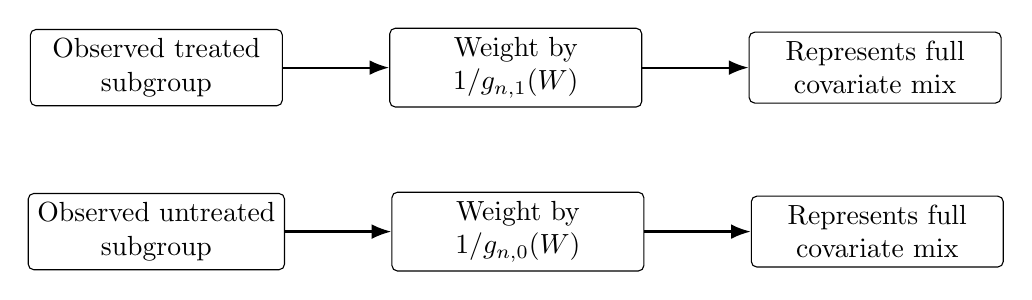
\begin{tikzpicture}[
  node distance=1.35cm,
  box/.style={draw, rounded corners=2pt, minimum width=3.2cm, minimum height=.8cm},
  arr/.style={-{Latex[length=2.5mm]}, thick}
]
\node[box] (obs) {Observed treated\\ subgroup};
\node[box, right=of obs] (weight) {Weight by\\ $1/g_{n,1}(W)$};
\node[box, right=of weight] (pseudo) {Represents full\\ covariate mix};
\draw[arr] (obs) -- (weight);
\draw[arr] (weight) -- (pseudo);
\node[box, below=1.1cm of obs] (obs0) {Observed untreated\\ subgroup};
\node[box, right=of obs0] (weight0) {Weight by\\ $1/g_{n,0}(W)$};
\node[box, right=of weight0] (pseudo0) {Represents full\\ covariate mix};
\draw[arr] (obs0) -- (weight0);
\draw[arr] (weight0) -- (pseudo0);
\end{tikzpicture}
\caption{IPTW reweights each observed treatment group to represent the target population.}
\label{fig:ch4-iptw-reweighting}
\end{figure}

Extreme weights arise when $g_{n,a}(W_i)$ is close to zero. Such observations can
dominate the estimate, which is why positivity is not merely a technical detail.

\subsection{Estimating $\E\{\Yone\}$, $\E\{\Yzero\}$, and the ATE}

Using the empirical joint distribution, the estimator simplifies to the individual-level
sample average
\[
\psi_n(a)
=
\frac{1}{n}\sum_{i=1}^n
\frac{\ind(A_i=a)}{g_{n,a}(W_i)}Y_i.
\]
The derivation follows by substituting the empirical distribution:
\[
\begin{aligned}
\sum_{w,a',y}
&\frac{\ind(a'=a)}{g_{n,a}(w)}
y\,P_n(W=w,A=a',Y=y)\\
&=
\sum_{w,a',y}
\frac{\ind(a'=a)}{g_{n,a}(w)}
y\left\{
\frac{1}{n}\sum_{i=1}^n
\ind(W_i=w,A_i=a',Y_i=y)
\right\}\\
&=
\frac{1}{n}\sum_{i=1}^n
\sum_{w,a',y}
\frac{\ind(a'=a)}{g_{n,a}(w)}
y\ind(W_i=w,A_i=a',Y_i=y)\\
&=
\frac{1}{n}\sum_{i=1}^n
\frac{\ind(A_i=a)}{g_{n,a}(W_i)}Y_i.
\end{aligned}
\]
Therefore,
\[
\psi_n(1)
=
\frac{1}{n}\sum_{i=1}^n
\frac{\ind(A_i=1)}{g_{n,1}(W_i)}Y_i,
\]
\[
\psi_n(0)
=
\frac{1}{n}\sum_{i=1}^n
\frac{\ind(A_i=0)}{g_{n,0}(W_i)}Y_i,
\]
and
\[
\widehat{\ATE}_{\IPTW}=\psi_n(1)-\psi_n(0).
\]

Using the same binary-$W$ summaries from empirical g-computation, suppose
\[
g_{n,1}(0)=0.476,\qquad g_{n,0}(0)=0.524,
\]
and
\[
g_{n,1}(1)=0.486,\qquad g_{n,0}(1)=0.514.
\]
The IPTW calculation weights each observed outcome by the inverse probability of
the treatment actually received. When the propensity scores are empirical stratum
proportions, the weighted treated mean reproduces the same standardized quantity
as empirical g-computation:
\[
\psi_n(1)=2.530,\qquad \psi_n(0)=2.392,
\]
and therefore
\[
\widehat{\ATE}_{\IPTW}=2.530-2.392=0.138.
\]
This numerical equality is a special property of the fully empirical discrete
estimator. It should not be expected once lower-dimensional regression smoothing is
used for $\Qbar_n$ or $g_n$.

\begin{implementationbox}
Regression-based IPTW in R:
\begin{lstlisting}[language=R]
fit_g <- glm(A ~ W, data = dat, family = binomial())

g1 <- predict(fit_g, type = "response")
g0 <- 1 - g1

psi1 <- mean((dat$A == 1) / g1 * dat$Y)
psi0 <- mean((dat$A == 0) / g0 * dat$Y)
ate  <- psi1 - psi0
\end{lstlisting}
\end{implementationbox}

\begin{estimationbox}
By-hand IPTW with discrete data:
\begin{enumerate}
\item Estimate $g_{n,1}(w)$ and $g_{n,0}(w)$ in every covariate stratum.
\item For each observation, compute $\omega_i(1)=\ind(A_i=1)/g_{n,1}(W_i)$ and
$\omega_i(0)=\ind(A_i=0)/g_{n,0}(W_i)$.
\item Compute $\psi_n(1)=n^{-1}\sum_i \omega_i(1)Y_i$.
\item Compute $\psi_n(0)=n^{-1}\sum_i \omega_i(0)Y_i$.
\item Subtract to estimate the ATE.
\end{enumerate}
\end{estimationbox}

\lecture{4.5}{Comparing G-Computation and IPTW}
\label{lec:4-5}

\subsection{When Empirical G-Computation and IPTW Coincide}

In the fully discrete setting, if both nuisance functions are estimated by empirical
subgroup proportions and means, empirical g-computation and empirical IPTW give the
same point estimate. This equality is not a general property of all g-computation and
IPTW estimators. It is a special algebraic feature of saturated discrete estimation.

\begin{proposition}[Equivalence under empirical discrete estimation]
Suppose $W$ is discrete, every relevant $(A=a,W=w)$ cell is nonempty, and
\[
\Qbar_n(a,w)
=
\frac{\sum_{i=1}^nY_i\ind(A_i=a,W_i=w)}
       {\sum_{i=1}^n\ind(A_i=a,W_i=w)},
\qquad
g_{n,a}(w)
=
\frac{\sum_{i=1}^n\ind(A_i=a,W_i=w)}
       {\sum_{i=1}^n\ind(W_i=w)}.
\]
Then
\[
\frac{1}{n}\sum_{i=1}^n \Qbar_n(a,W_i)
=
\frac{1}{n}\sum_{i=1}^n
\frac{\ind(A_i=a)}{g_{n,a}(W_i)}Y_i.
\]
\end{proposition}

\begin{proof}
Let $n_w=\sum_i\ind(W_i=w)$ and $n_{aw}=\sum_i\ind(A_i=a,W_i=w)$.
The g-computation estimator can be written as
\[
\sum_w \Qbar_n(a,w)\frac{n_w}{n}.
\]
Substituting the empirical subgroup mean,
\[
\sum_w
\left\{
\frac{\sum_iY_i\ind(A_i=a,W_i=w)}{n_{aw}}
\right\}
\frac{n_w}{n}.
\]
Substituting $g_{n,a}(w)=n_{aw}/n_w$ gives
\[
\frac{1}{n}\sum_w
\sum_i
Y_i\ind(A_i=a,W_i=w)
\frac{1}{g_{n,a}(w)}.
\]
For each observation $i$, only the term with $w=W_i$ contributes, so the expression
equals
\[
\frac{1}{n}\sum_{i=1}^n
\frac{\ind(A_i=a)}{g_{n,a}(W_i)}Y_i,
\]
which is the IPTW estimator.
\end{proof}

\subsection{Why the Equivalence Is Special}

The proof above uses two facts. First, $\Qbar_n(a,w)$ is the empirical mean in exactly
the same strata used to estimate $g_{n,a}(w)$. Second, the empirical covariate
distribution gives each stratum weight $n_w/n$. If either nuisance function is
estimated by a model that smooths across strata, the exact cancellation in the proof
usually disappears.

\begin{keyidea}
G-computation and IPTW are equivalent as identification formulas under the causal
assumptions. Their finite-sample estimators need not be equal, because the fitted
outcome regression and fitted propensity score can approximate different parts of the
observed-data distribution in different ways.
\end{keyidea}

\begin{figure}[H]
\centering
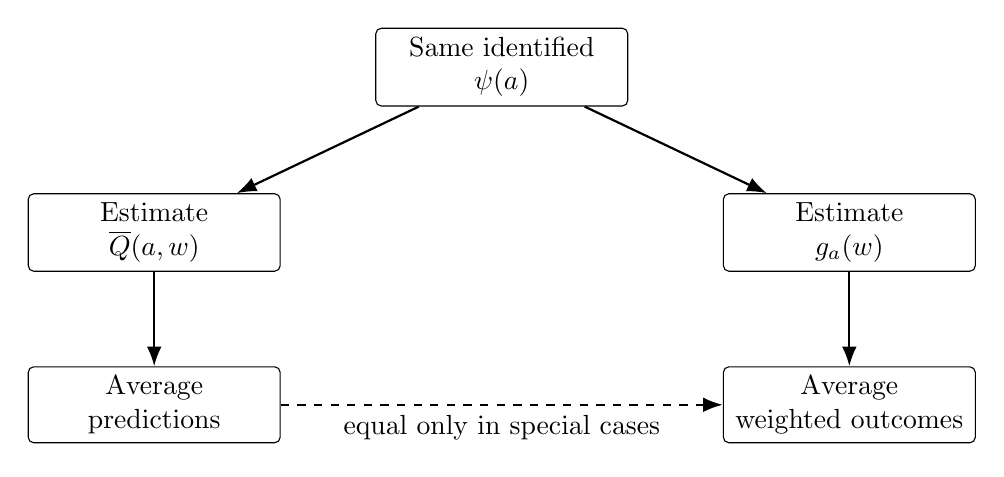
\begin{tikzpicture}[
  node distance=1.45cm,
  box/.style={draw, rounded corners=2pt, minimum width=3.2cm, minimum height=.8cm},
  arr/.style={-{Latex[length=2.5mm]}, thick}
]
\node[box] (id) {Same identified\\ $\psi(a)$};
\node[box, below left=1.1cm and 1.2cm of id] (gcomp) {Estimate\\ $\Qbar(a,w)$};
\node[box, below right=1.1cm and 1.2cm of id] (iptw) {Estimate\\ $g_a(w)$};
\node[box, below=1.2cm of gcomp] (pg) {Average\\ predictions};
\node[box, below=1.2cm of iptw] (pi) {Average\\ weighted outcomes};
\draw[arr] (id) -- (gcomp);
\draw[arr] (id) -- (iptw);
\draw[arr] (gcomp) -- (pg);
\draw[arr] (iptw) -- (pi);
\draw[arr, dashed] (pg) -- node[below] {equal only in special cases} (pi);
\end{tikzpicture}
\caption{The two methods estimate the same causal parameter through different nuisance functions.}
\label{fig:ch4-gcomp-iptw-comparison}
\end{figure}

\subsection{High-Dimensional Discrete Covariates}

Empirical stratification becomes fragile when $W$ has many discrete components.
If $W=(W_1,\ldots,W_p)$ and each $W_j$ is binary, then $W$ can take $2^p$ possible
values. Even moderate $p$ can create many sparse or empty strata.

Sparse strata create two problems. For g-computation, $\Qbar_n(a,w)$ is unstable when
only a few observations have $A=a$ and $W=w$, and undefined when no such observation
exists. For IPTW, $g_{n,a}(w)$ is unstable when treatment counts are small, and the
weights $1/g_{n,a}(w)$ can become extremely large.

\subsection{Continuous Covariates}

If $W$ contains a continuous component, exact empirical stratification usually fails.
In a continuous distribution, the probability that two individuals have exactly the
same covariate vector is often zero. Then the subgroup
\[
\{i:W_i=w\}
\]
may contain only one observation or none, making empirical subgroup means unusable.

This is not a conceptual problem for the estimand. The counterfactual mean
\[
\psi(a)=\E\{\Qbar(a,W)\}
\]
is still well-defined. The difficulty is statistical: we must estimate the smooth
conditional mean or treatment probability from finite data.

\subsection{Need for Regression Smoothing}

Regression smoothing borrows information across similar covariate values. Instead of
estimating a separate mean for every exact $w$, a model might assume
\[
\Qbar(a,w)=\beta_0+\beta_1a+\beta_2^\top w
\]
or
\[
g_1(w)=\expit(\alpha_0+\alpha_1^\top w).
\]
These restrictions reduce variance, but they introduce the possibility of model
misspecification. A simple main-terms model may be too rigid if the true outcome
regression has nonlinearities or treatment-covariate interactions.

The central estimation tradeoff is therefore:
\[
\text{less smoothing} \Rightarrow \text{lower modeling bias but higher variance},
\]
\[
\text{more smoothing} \Rightarrow \text{lower variance but higher risk of bias}.
\]

\subsection{Variance and Instability}

IPTW estimators are especially sensitive to near-violations of positivity. If
$g_{n,1}(W_i)=0.02$, then a treated individual receives weight $50$. A small number of
such observations can strongly influence the weighted mean.

G-computation can also be unstable or biased, but the failure mode is different. A
poor outcome regression may extrapolate into covariate-treatment combinations with
little support. For example, if very old individuals are almost never treated, then
$\Qbar_n(1,w)$ for very old $w$ is largely determined by model assumptions rather
than direct data.

\begin{estimationbox}
Practical comparison:
\begin{itemize}
\item Empirical g-computation and empirical IPTW coincide in low-dimensional
discrete settings with nonempty cells.
\item Regression-based g-computation and regression-based IPTW usually differ.
\item G-computation relies most directly on the quality of the outcome regression.
\item IPTW relies most directly on the quality of the propensity score and on stable
positivity.
\item Large weights, empty cells, and extrapolation are diagnostic signs that the
data may not contain enough information for the desired causal contrast without
strong modeling assumptions.
\end{itemize}
\end{estimationbox}

\lecture{4.6}{G-Computation and IPTW in R}
\label{lec:4-6}

\subsection{Data Preparation}

The R implementations of g-computation and IPTW are most reliable when the data are
prepared so that the notation matches the analysis. The dataset should contain one row
per individual and variables corresponding to $W$, $A$, and $Y$:
\[
O_i=(W_i,A_i,Y_i).
\]
Treatment should be coded consistently, often as $A=1$ for treated and $A=0$ for
untreated. Binary outcomes should also be coded as $0/1$ when logistic regression is
used.

\begin{implementationbox}
Example setup:
\begin{lstlisting}[language=R]
# dat has one row per individual
# A: binary treatment, coded 0/1
# Y: outcome
# W1, W2: pre-treatment covariates

dat <- dat[complete.cases(dat[, c("Y", "A", "W1", "W2")]), ]
dat$A <- as.numeric(dat$A == 1)
dat$Y <- as.numeric(dat$Y)
\end{lstlisting}
\end{implementationbox}

Dropping observations with missing data is simple but not always appropriate. If
missingness is related to treatment, outcome, or covariates, complete-case analysis can
change the target population or introduce bias. Later chapters treat missing data more
carefully.

\subsection{Fitting Outcome Regressions}

For g-computation, the nuisance function is
\[
\Qbar(a,w)=\E(Y\given A=a,W=w).
\]
The fitted outcome regression should include treatment and the confounders required
for identification. It may also include interactions or nonlinear terms if scientifically
or statistically warranted.

\begin{implementationbox}
Outcome regression examples:
\begin{lstlisting}[language=R]
# Continuous outcome, identity link
fit_Q_linear <- glm(Y ~ A + W1 + W2, data = dat, family = gaussian())

# Binary outcome, logistic link
fit_Q_logistic <- glm(Y ~ A + W1 + W2, data = dat, family = binomial())

# Interaction model allowing treatment effect heterogeneity by W1
fit_Q_interact <- glm(Y ~ A * W1 + W2, data = dat, family = binomial())
\end{lstlisting}
\end{implementationbox}

The fitted object is not itself the causal estimate. It is an estimate of a nuisance
function used to compute predicted counterfactual outcomes.

\subsection{Fitting Propensity Score Models}

For IPTW, the nuisance function is
\[
g_1(w)=\Prob(A=1\given W=w).
\]
Because $A$ is binary, logistic regression is a common starting point:
\[
\logit\{g_1(w)\}=\alpha_0+\alpha^\top w.
\]

\begin{implementationbox}
Propensity score model:
\begin{lstlisting}[language=R]
fit_g <- glm(A ~ W1 + W2, data = dat, family = binomial())

g1 <- predict(fit_g, type = "response")
g0 <- 1 - g1
\end{lstlisting}
\end{implementationbox}

After fitting the propensity score, inspect whether predicted probabilities are close
to zero or one. Very small $g_1(W_i)$ among treated individuals or very small
$g_0(W_i)$ among untreated individuals lead to large IPTW weights.

\subsection{Prediction Workflows}

The g-computation prediction workflow constructs the two estimated counterfactual
means by changing only the treatment variable:

\[
\psi_n(1)=\frac{1}{n}\sum_{i=1}^n\Qbar_n(1,W_i),
\qquad
\psi_n(0)=\frac{1}{n}\sum_{i=1}^n\Qbar_n(0,W_i).
\]

\begin{implementationbox}
G-computation prediction workflow:
\begin{lstlisting}[language=R]
dat1 <- dat
dat1$A <- 1

dat0 <- dat
dat0$A <- 0

Q1 <- predict(fit_Q_logistic, newdata = dat1, type = "response")
Q0 <- predict(fit_Q_logistic, newdata = dat0, type = "response")

psi1_gcomp <- mean(Q1)
psi0_gcomp <- mean(Q0)
ate_gcomp  <- psi1_gcomp - psi0_gcomp
\end{lstlisting}
\end{implementationbox}

For IPTW, no treatment-specific prediction datasets are required. The estimator uses
the observed treatment and observed outcome:
\[
\psi_n^{\IPTW}(a)=
\frac{1}{n}\sum_{i=1}^n
\frac{\ind(A_i=a)}{g_{n,a}(W_i)}Y_i.
\]

\begin{implementationbox}
IPTW workflow:
\begin{lstlisting}[language=R]
A <- dat$A
Y <- dat$Y

psi1_iptw <- mean((A == 1) / g1 * Y)
psi0_iptw <- mean((A == 0) / g0 * Y)
ate_iptw  <- psi1_iptw - psi0_iptw
\end{lstlisting}
\end{implementationbox}

\subsection{Treatment-Specific Datasets}

Treatment-specific datasets are useful because they make the estimand visible in the
code. The dataset \texttt{dat1} represents the empirical covariate distribution with
everyone assigned $A=1$; \texttt{dat0} represents the same empirical covariate
distribution with everyone assigned $A=0$.

\begin{figure}[H]
\centering
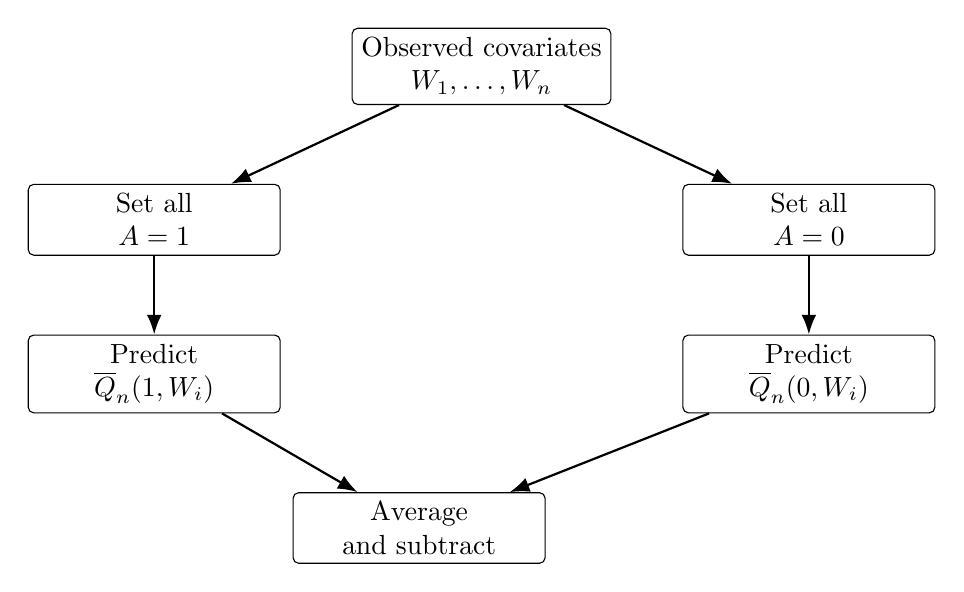
\begin{tikzpicture}[
  node distance=1.35cm,
  box/.style={draw, rounded corners=2pt, minimum width=3.2cm, minimum height=.8cm},
  arr/.style={-{Latex[length=2.5mm]}, thick}
]
\node[box] (dat) {Observed covariates\\ $W_1,\ldots,W_n$};
\node[box, below left=1cm and .9cm of dat] (dat1) {Set all\\ $A=1$};
\node[box, below right=1cm and .9cm of dat] (dat0) {Set all\\ $A=0$};
\node[box, below=1cm of dat1] (q1) {Predict\\ $\Qbar_n(1,W_i)$};
\node[box, below=1cm of dat0] (q0) {Predict\\ $\Qbar_n(0,W_i)$};
\node[box, below right=1cm and .15cm of q1] (ate) {Average\\ and subtract};
\draw[arr] (dat) -- (dat1);
\draw[arr] (dat) -- (dat0);
\draw[arr] (dat1) -- (q1);
\draw[arr] (dat0) -- (q0);
\draw[arr] (q1) -- (ate);
\draw[arr] (q0) -- (ate);
\end{tikzpicture}
\caption{Treatment-specific datasets implement g-computation predictions.}
\label{fig:ch4-treatment-specific-data}
\end{figure}

This workflow should not be confused with changing the observed data. The original
outcomes remain the data used to fit the outcome model. The modified datasets are
only prediction grids used to evaluate the fitted conditional mean.

\subsection{Practical Implementation Patterns}

It is often helpful to wrap estimators in functions. This makes bootstrap inference
straightforward and reduces the chance of accidentally using variables from the wrong
dataset.

\begin{implementationbox}
Reusable g-computation function:
\begin{lstlisting}[language=R]
get_gcomp <- function(input_data) {
  fit_Q <- glm(Y ~ A + W1 + W2, data = input_data, family = binomial())

  data1 <- input_data
  data1$A <- 1
  data0 <- input_data
  data0$A <- 0

  Q1 <- predict(fit_Q, newdata = data1, type = "response")
  Q0 <- predict(fit_Q, newdata = data0, type = "response")

  c(psi0 = mean(Q0), psi1 = mean(Q1), ate = mean(Q1) - mean(Q0))
}
\end{lstlisting}
\end{implementationbox}

\begin{implementationbox}
Reusable IPTW function:
\begin{lstlisting}[language=R]
get_iptw <- function(input_data) {
  fit_g <- glm(A ~ W1 + W2, data = input_data, family = binomial())

  g1 <- predict(fit_g, type = "response")
  g0 <- 1 - g1

  A <- input_data$A
  Y <- input_data$Y

  psi1 <- mean((A == 1) / g1 * Y)
  psi0 <- mean((A == 0) / g0 * Y)

  c(psi0 = psi0, psi1 = psi1, ate = psi1 - psi0)
}
\end{lstlisting}
\end{implementationbox}

\begin{estimationbox}
Implementation checks:
\begin{itemize}
\item Confirm that $A$, $Y$, and all covariates are coded as intended.
\item For g-computation, confirm that \texttt{newdata} contains the same covariate
names and factor levels as the model-fitting dataset.
\item For IPTW, inspect summaries of $g_1$, $g_0$, and the resulting weights.
\item Keep the estimation function self-contained so that resampling methods refit
all nuisance functions inside each resampled dataset.
\end{itemize}
\end{estimationbox}

\lecture{4.7}{Bootstrap Inference}
\label{lec:4-7}

\subsection{Why Variance Formulas Are Complex}

Point estimates alone are not enough. A causal analysis should also report uncertainty:
standard errors, confidence intervals, and sometimes hypothesis tests. For
g-computation and IPTW, uncertainty comes from several sources at once.

For g-computation, the estimator
\[
\psi_n^{\mathrm{gcomp}}(a)
=
\frac{1}{n}\sum_{i=1}^n \Qbar_n(a,W_i)
\]
depends on the empirical distribution of $W$ and on the fitted outcome regression
$\Qbar_n$. For IPTW, the estimator
\[
\psi_n^{\IPTW}(a)
=
\frac{1}{n}\sum_{i=1}^n
\frac{\ind(A_i=a)}{g_{n,a}(W_i)}Y_i
\]
depends on the empirical distribution of $(W,A,Y)$ and on the fitted propensity score
$g_{n,a}$. Treating $\Qbar_n$ or $g_n$ as fixed after fitting usually understates
uncertainty because it ignores the fact that the nuisance functions were estimated
from the same data.

\begin{keyidea}
The standard error must reflect the entire estimation procedure, not only the final
sample average. When nuisance functions are fit from data, their variability is part
of the variability of the causal effect estimator.
\end{keyidea}

\subsection{Nonparametric Bootstrap}

The nonparametric bootstrap approximates repeated sampling by resampling the observed
data. Let $\psi_n$ denote an estimator of a counterfactual mean or ATE. A bootstrap
replicate is constructed as follows:

\begin{enumerate}
\item Sample $n$ rows from the original dataset with replacement.
\item Refit all nuisance models in this bootstrap dataset.
\item Recompute the complete estimator in the bootstrap dataset.
\end{enumerate}

Repeating these steps $M$ times gives bootstrap estimates
\[
\psi_n^{\#,1},\psi_n^{\#,2},\ldots,\psi_n^{\#,M}.
\]
The symbol $\#$ is used here to distinguish bootstrap estimates from the original
estimate $\psi_n$.

\begin{figure}[H]
\centering
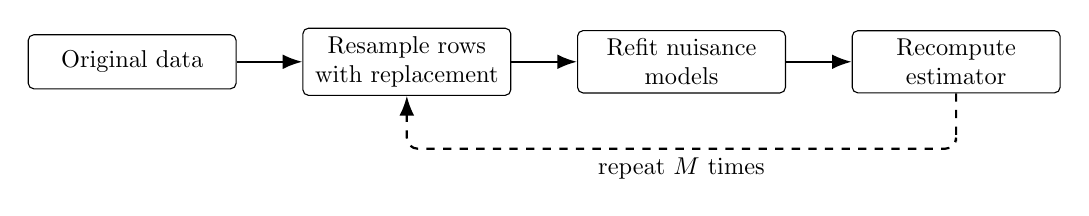
\begin{tikzpicture}[
  scale=.88,
  transform shape,
  node distance=.95cm,
  box/.style={draw, rounded corners=2pt, minimum width=3.0cm, minimum height=.78cm},
  arr/.style={-{Latex[length=2.5mm]}, thick}
]
\node[box] (data) {Original data};
\node[box, right=of data] (resample) {Resample rows\\ with replacement};
\node[box, right=of resample] (refit) {Refit nuisance\\ models};
\node[box, right=of refit] (estimate) {Recompute\\ estimator};
\draw[arr] (data) -- (resample);
\draw[arr] (resample) -- (refit);
\draw[arr] (refit) -- (estimate);
\draw[arr, rounded corners, dashed] (estimate.south) |- ++(0,-.8) -| node[below,pos=.25] {repeat $M$ times} (resample.south);
\end{tikzpicture}
\caption{Each bootstrap replicate repeats the full estimation procedure.}
\label{fig:ch4-bootstrap-flow}
\end{figure}

\subsection{Bootstrap Confidence Intervals}

A percentile bootstrap confidence interval uses quantiles of the bootstrap estimates.
For a nominal 95\% interval, let $\psi_n^\#(0.025)$ and $\psi_n^\#(0.975)$ be the
empirical 2.5th and 97.5th percentiles of
$\psi_n^{\#,1},\ldots,\psi_n^{\#,M}$. The interval is
\[
\left[
\psi_n^\#(0.025),\ \psi_n^\#(0.975)
\right].
\]
This interval is easy to compute and often adequate for introductory analyses, but it
can perform poorly in small samples, with highly skewed estimators, or when the
estimator is irregular.

\subsection{Bootstrap Standard Errors}

The bootstrap standard error is the sample standard deviation of the bootstrap
estimates:
\[
\hat\sigma^\#
=
\left[
\frac{1}{M-1}\sum_{m=1}^M
\left(\psi_n^{\#,m}-\bar\psi_n^\#\right)^2
\right]^{1/2},
\]
where
\[
\bar\psi_n^\#=\frac{1}{M}\sum_{m=1}^M \psi_n^{\#,m}.
\]
This standard error can be reported directly or used in Wald-style confidence
intervals of the form
\[
\psi_n\pm 1.96\,\hat\sigma^\#.
\]

\subsection{Wald-Style p-Values}

For testing
\[
H_0:\psi=0
\qquad\text{versus}\qquad
H_1:\psi\neq 0,
\]
a Wald-style test statistic is
\[
Z=\frac{\psi_n}{\hat\sigma^\#}.
\]
Using the standard normal approximation, the two-sided p-value is
\[
p=2\left\{1-\Phi(|Z|)\right\},
\]
where $\Phi$ is the cumulative distribution function of the standard normal
distribution.

This p-value inherits the assumptions of the large-sample approximation and the
bootstrap standard error. It should be interpreted as a statistical summary, not as a
measure of whether the causal assumptions are true.

\subsection{Bootstrap for G-Computation}

The key rule is that the outcome regression must be refit in every bootstrap sample.
If the fitted model from the original data is reused, the bootstrap will miss an
important component of uncertainty.

\begin{implementationbox}
Bootstrap for g-computation:
\begin{lstlisting}[language=R]
get_gcomp <- function(input_data) {
  fit_Q <- glm(Y ~ A + W1 + W2, data = input_data, family = binomial())

  data1 <- input_data
  data1$A <- 1
  data0 <- input_data
  data0$A <- 0

  Q1 <- predict(fit_Q, newdata = data1, type = "response")
  Q0 <- predict(fit_Q, newdata = data0, type = "response")

  psi1 <- mean(Q1)
  psi0 <- mean(Q0)
  c(psi0 = psi0, psi1 = psi1, ate = psi1 - psi0)
}

set.seed(1234)
M <- 1000
n <- nrow(dat)

boot_ate <- numeric(M)

for (m in seq_len(M)) {
  boot_ids <- sample(seq_len(n), size = n, replace = TRUE)
  boot_dat <- dat[boot_ids, ]
  boot_ate[m] <- get_gcomp(boot_dat)["ate"]
}

est <- get_gcomp(dat)["ate"]
se_boot <- sd(boot_ate)
ci_boot <- quantile(boot_ate, probs = c(0.025, 0.975))
p_value <- 2 * pnorm(-abs(est / se_boot))
\end{lstlisting}
\end{implementationbox}

The same bootstrap draws can be used to compute confidence intervals for
$\psi(0)$, $\psi(1)$, and the ATE if the function returns all three quantities.

\subsection{Bootstrap for IPTW}

For IPTW, the propensity score model must be refit in every bootstrap sample. The
weights in each bootstrap replicate should be computed from the bootstrap-fitted
propensity scores, not from the original fitted propensity scores.

\begin{implementationbox}
Bootstrap for IPTW:
\begin{lstlisting}[language=R]
get_iptw <- function(input_data) {
  fit_g <- glm(A ~ W1 + W2, data = input_data, family = binomial())

  g1 <- predict(fit_g, type = "response")
  g0 <- 1 - g1

  A <- input_data$A
  Y <- input_data$Y

  psi1 <- mean((A == 1) / g1 * Y)
  psi0 <- mean((A == 0) / g0 * Y)
  c(psi0 = psi0, psi1 = psi1, ate = psi1 - psi0)
}

set.seed(1234)
M <- 1000
n <- nrow(dat)

boot_ate <- numeric(M)

for (m in seq_len(M)) {
  boot_ids <- sample(seq_len(n), size = n, replace = TRUE)
  boot_dat <- dat[boot_ids, ]
  boot_ate[m] <- get_iptw(boot_dat)["ate"]
}

est <- get_iptw(dat)["ate"]
se_boot <- sd(boot_ate)
ci_boot <- quantile(boot_ate, probs = c(0.025, 0.975))
p_value <- 2 * pnorm(-abs(est / se_boot))
\end{lstlisting}
\end{implementationbox}

\begin{estimationbox}
Bootstrap checklist:
\begin{itemize}
\item Resample rows, not individual variables independently.
\item Refit every nuisance model inside each bootstrap sample.
\item Recompute the entire estimator from the resampled data.
\item Use enough bootstrap replicates for stable quantiles; $M=1000$ is a common
minimum for routine work.
\item Inspect failed model fits, separation warnings, and extreme weights, because
these are informative signs of instability.
\end{itemize}
\end{estimationbox}


\chapterheading{5}{Super Learning}
\lecture{5.1}{Why Flexible Regression Is Needed}
\label{lec:5-1}

\subsection{Limitations of Empirical Moment Estimators}

The g-computation and IPTW estimators from Chapter 4 require nuisance functions:
\[
\Qbar(a,w)=\E(Y\given A=a,W=w),
\qquad
g_a(w)=\Prob(A=a\given W=w).
\]
When $W$ is low-dimensional and discrete, these functions can be estimated by
empirical subgroup means and proportions. For example,
\[
\Qbar_n(a,w)=
\frac{\sum_{i=1}^nY_i\ind(A_i=a,W_i=w)}
     {\sum_{i=1}^n\ind(A_i=a,W_i=w)}
\]
is reasonable if there are enough observations in every treatment-covariate stratum.

This approach fails as soon as the number of strata is large relative to the sample
size. If $W$ contains ten binary variables, there are $2^{10}=1024$ possible covariate
patterns before treatment is even considered. Many cells will be empty, and many
nonempty cells will contain too few observations to estimate a stable conditional mean.
The same problem affects the propensity score: a stratum with only one treated and no
untreated individuals cannot support both $g_1(w)$ and $g_0(w)$ empirically.

\begin{keyidea}
Empirical moment estimators are transparent but local. They use only observations
with exactly the same covariate values. That is attractive in small discrete examples,
but it becomes unstable or undefined when covariates are high-dimensional or
continuous.
\end{keyidea}

\subsection{Continuous Covariates}

Continuous covariates make exact stratification especially problematic. Suppose $W$
is body mass index or age measured in years and decimals. In a continuous
distribution, the probability that two people have exactly the same value of $W$ is
often close to zero. Then the empirical subgroup
\[
\{i:W_i=w\}
\]
is empty for most values $w$ and may contain only one individual at observed values.

The target function $\Qbar(a,w)$ is still meaningful. The question
\[
\E(Y\given A=1,W=-3.5)
\]
asks for the average outcome among treated individuals with covariate value $-3.5$.
The problem is not conceptual; it is statistical. A finite sample does not contain many
people with exactly that covariate value, so we need a method that uses information
from nearby or otherwise similar covariate values.

\subsection{Borrowing Information Across Covariate Values}

To estimate $\Qbar(a,w)$ at a particular $w$, we must decide which observations are
informative about that point. Observations with covariates very close to $w$ are
usually more relevant than observations far away from $w$, but using only the closest
observations can produce a noisy estimate.

The same issue appears for the propensity score. To estimate
\[
g_1(w)=\Prob(A=1\given W=w),
\]
we need to learn how treatment probabilities vary with $W$. If we use only people
with exactly $W=w$, the estimate is unstable. If we use everyone equally, the estimate
may ignore important differences in treatment assignment across covariates.

\begin{figure}[H]
\centering
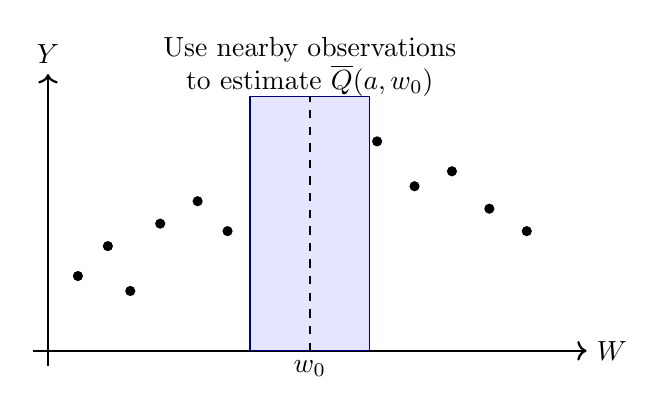
\begin{tikzpicture}[
  scale=.95,
  axis/.style={->, thick},
  pt/.style={circle, fill=black, inner sep=1.3pt},
  window/.style={fill=blue!10, draw=blue!50!black},
  arr/.style={-{Latex[length=2.5mm]}, thick}
]
\draw[axis] (-.2,0) -- (7.2,0) node[right] {$W$};
\draw[axis] (0,-.2) -- (0,3.7) node[above] {$Y$};
\foreach \x/\y in {.4/1.0,.8/1.4,1.1/.8,1.5/1.7,2.0/2.0,2.4/1.6,2.8/2.4,3.2/2.7,3.5/2.5,3.9/2.9,4.4/2.8,4.9/2.2,5.4/2.4,5.9/1.9,6.4/1.6}
  \node[pt] at (\x,\y) {};
\draw[window] (2.7,0) rectangle (4.3,3.4);
\draw[dashed, thick] (3.5,0) -- (3.5,3.4);
\node[below] at (3.5,0) {$w_0$};
\node[align=center] at (3.5,3.8) {Use nearby observations\\to estimate $\Qbar(a,w_0)$};
\end{tikzpicture}
\caption{Flexible regression borrows information across covariate values.}
\label{fig:ch5-borrowing}
\end{figure}

\subsection{Regression as Smoothing}

Regression is a formal way to borrow information. A regression estimator smooths the
observed outcomes across covariate values in order to estimate a conditional mean
function. The amount and shape of smoothing depend on the method.

A linear regression with
\[
\Qbar(a,w)=\beta_0+\beta_1a+\beta_2w
\]
borrows information very aggressively. The model assumes that a one-unit change in
$W$ has the same additive association with $Y$ everywhere. If this is true, the method
can be efficient. If it is false, the method may be biased.

A kernel regression borrows information locally. It estimates $\Qbar(a,w)$ using
observations whose covariates are close to $w$. A regression tree borrows information
within leaves of a fitted tree. A random forest averages many such trees. A generalized
additive model borrows information through smooth functions of predictors. Each
method embodies a different answer to the same question: which observations should
inform the prediction at a given covariate value, and how much should they count?

\subsection{Why Model Choice Matters for Causal Estimators}

In causal inference, nuisance regression quality matters because causal estimators are
functions of these regressions. For g-computation,
\[
\widehat{\ATE}_{\mathrm{gcomp}}
=
\frac{1}{n}\sum_{i=1}^n
\left\{\Qbar_n(1,W_i)-\Qbar_n(0,W_i)\right\}.
\]
If $\Qbar_n$ is biased in regions of the covariate space that are common in the target
population, the ATE estimate can be biased.

For IPTW,
\[
\widehat{\ATE}_{\IPTW}
=
\frac{1}{n}\sum_{i=1}^n
\left\{
\frac{\ind(A_i=1)}{g_{n,1}(W_i)}Y_i
-
\frac{\ind(A_i=0)}{g_{n,0}(W_i)}Y_i
\right\}.
\]
If $g_n$ is poorly estimated, the weights can be wrong, unstable, or both.

\begin{assumptionbox}
Flexible regression does not replace causal assumptions. Consistency,
conditional randomization, and positivity are still required to interpret the resulting
statistical estimates causally. Super Learning helps estimate observed-data nuisance
functions; it does not make unmeasured confounding disappear.
\end{assumptionbox}

\begin{estimationbox}
The practical objective in this chapter is to estimate nuisance functions well enough
for causal estimation. We therefore need a principled way to compare candidate
regression estimators before using them inside g-computation, IPTW, or later doubly
robust estimators.
\end{estimationbox}

\lecture{5.2}{Bias--Variance Tradeoff}
\label{lec:5-2}

\subsection{Low Bias vs High Variance}

Bias and variance describe two different ways an estimator can perform poorly.
Suppose the target regression function is
\[
Q_0(a,w)=\E(Y\given A=a,W=w),
\]
and $\Qbar_n(a,w)$ is an estimator computed from a sample. At a fixed point
$(a,w)$, the bias is the difference between the average value of the estimator across
repeated samples and the truth:
\[
\Bias\{\Qbar_n(a,w)\}
=
\E\{\Qbar_n(a,w)\}-Q_0(a,w).
\]
The variance describes how much $\Qbar_n(a,w)$ changes from sample to sample:
\[
\Var\{\Qbar_n(a,w)\}
=
\E\left[
\left\{\Qbar_n(a,w)-\E\{\Qbar_n(a,w)\}\right\}^2
\right].
\]

An estimator can have low bias but high variance. For example, an estimator that uses
only people with covariates extremely close to $w$ may target the local conditional
mean accurately, but because it uses very few observations, its estimate can fluctuate
substantially across samples.

\subsection{High Bias vs Low Variance}

An estimator can also have high bias but low variance. A simple linear regression may
use the full sample and therefore produce stable estimates. But if the true regression
function is strongly nonlinear, the fitted line may systematically miss the truth.

\begin{keyidea}
Bias is systematic error from using a method that is too rigid or otherwise wrong.
Variance is random error from using a method that is too sensitive to the particular
sample. Good prediction requires balancing both.
\end{keyidea}

\subsection{Kernel Regression Intuition}

Kernel regression provides a concrete picture of the bias-variance tradeoff. Consider
estimating $\E(Y\given A=1,W=w_0)$. A simple local estimator is the uniform-kernel
estimator
\[
\Qbar_{n,h}(1,w_0)
=
\frac{\sum_{i=1}^nY_i\ind(A_i=1)\ind(|W_i-w_0|\le h/2)}
       {\sum_{i=1}^n\ind(A_i=1)\ind(|W_i-w_0|\le h/2)}.
\]
The tuning parameter $h>0$ is the bandwidth. The estimator averages outcomes among
treated individuals whose $W$ values fall inside a window of width $h$ centered at
$w_0$.

If $h$ is small, the estimator uses only very similar people. That reduces bias when
the regression function changes with $W$, but it increases variance because the
estimate is based on fewer observations. If $h$ is large, the estimator uses more
people. That reduces variance but may introduce bias by averaging over people who are
not very similar to $w_0$.

\subsection{Bandwidth Choice}

Bandwidth choice is a model selection problem. There is no universally best
bandwidth because the optimal choice depends on the unknown smoothness of the true
regression function and on the sample size. A very smooth true function can tolerate a
larger bandwidth. A highly curved true function requires a smaller bandwidth to avoid
oversmoothing.

\begin{figure}[H]
\centering
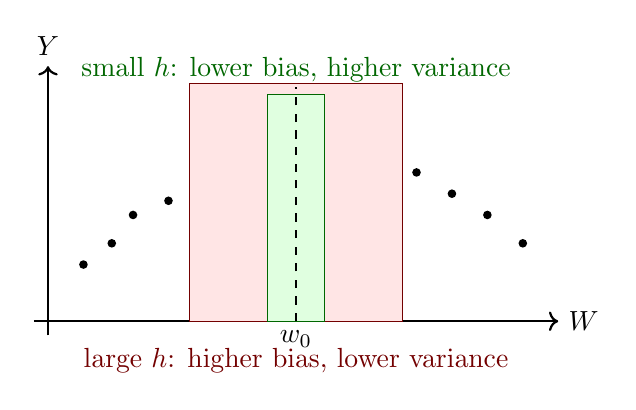
\begin{tikzpicture}[
  scale=.9,
  axis/.style={->, thick},
  pt/.style={circle, fill=black, inner sep=1.1pt},
  small/.style={fill=green!12, draw=green!40!black},
  large/.style={fill=red!10, draw=red!45!black}
]
\draw[axis] (-.2,0) -- (7.2,0) node[right] {$W$};
\draw[axis] (0,-.2) -- (0,3.6) node[above] {$Y$};
\foreach \x/\y in {.5/.8,.9/1.1,1.2/1.5,1.7/1.7,2.1/2.0,2.6/2.4,3.0/2.6,3.4/2.8,3.8/2.7,4.2/2.5,4.7/2.4,5.2/2.1,5.7/1.8,6.2/1.5,6.7/1.1}
  \node[pt] at (\x,\y) {};
\draw[large] (2.0,0) rectangle (5.0,3.35);
\draw[small] (3.1,0) rectangle (3.9,3.2);
\draw[dashed, thick] (3.5,0) -- (3.5,3.3);
\node[below] at (3.5,0) {$w_0$};
\node[green!40!black] at (3.5,3.55) {small $h$: lower bias, higher variance};
\node[red!45!black] at (3.5,-.55) {large $h$: higher bias, lower variance};
\end{tikzpicture}
\caption{The bandwidth controls how much information is borrowed across covariate values.}
\label{fig:ch5-bandwidth}
\end{figure}

\subsection{Parametric vs Semiparametric vs Nonparametric Methods}

Regression methods differ in how strongly they restrict the true regression function.

\begin{definition}[Parametric method]
A parametric regression method assumes that the regression function belongs to a
finite-dimensional family, such as
\[
\Qbar(a,w)=\beta_0+\beta_1a+\beta_2^\top w.
\]
\end{definition}

Parametric methods can have low variance because they impose strong structure, but
they can have high bias if the structure is wrong.

\begin{definition}[Semiparametric method]
A semiparametric method combines finite-dimensional components with flexible
components. For example,
\[
\Qbar(a,w)=\beta_0+\beta_1a+f(w)
\]
leaves the function $f$ unspecified or only weakly restricted.
\end{definition}

\begin{definition}[Nonparametric method]
A nonparametric method allows the regression function to become increasingly
flexible as the sample size grows. Examples include kernel regression, random
forests, neural networks, and certain spline or tree-based methods.
\end{definition}

The labels are less important than the practical consequence: different methods
borrow information in different ways and therefore occupy different points in the
bias-variance tradeoff.

\subsection{Unknown True Regression Function}

If the true regression function were known to be linear, a linear model would be a
natural choice. If the true function were known to have sharp interactions, a more
adaptive method would be needed. In practice, the true function is unknown.

This uncertainty is the motivation for Super Learning. Rather than choosing one
regression method because it is familiar, we pre-specify a library of plausible
candidate methods and use cross-validated risk to compare them.

\begin{estimationbox}
For causal estimation, model choice is not merely a prediction issue. Bias in
$\Qbar_n$ can bias g-computation; instability in $g_n$ can destabilize IPTW. The
next lectures develop a risk-based framework for choosing or combining nuisance
function estimators.
\end{estimationbox}

\lecture{5.3}{Risk and Loss Functions}
\label{lec:5-3}

\subsection{Prediction Loss}

To compare regression estimators, we need a numerical score. A loss function measures
how bad a prediction is for one observation. If $\Qbar_n$ predicts the outcome using
$A$ and $W$, then a loss function assigns a number
\[
L(\Qbar_n)(W,A,Y)
\]
to the prediction-observation pair. Smaller loss means better prediction.

The choice of loss should match the regression target. If the target is the conditional
mean of a continuous outcome, squared-error loss is natural. If the target is the
conditional probability of a binary outcome, negative log-likelihood loss is natural.

\subsection{Squared-Error Loss}

For a continuous or mean-valued outcome regression, squared-error loss is
\[
L(\Qbar_n)(w,a,y)
=
\{y-\Qbar_n(a,w)\}^2.
\]
This loss heavily penalizes large prediction errors because the error is squared. It is
the standard loss for estimating conditional means.

\subsection{Negative Log-Likelihood Loss}

For a binary outcome $Y\in\{0,1\}$, an outcome regression estimates
\[
\Qbar(a,w)=\Prob(Y=1\given A=a,W=w).
\]
If $\Qbar_n(a,w)$ is a predicted probability, the Bernoulli likelihood contribution is
\[
\Qbar_n(a,w)^y\{1-\Qbar_n(a,w)\}^{1-y}.
\]
The negative log-likelihood loss is
\[
L(\Qbar_n)(w,a,y)
=
-\log\left[
\Qbar_n(a,w)^y\{1-\Qbar_n(a,w)\}^{1-y}
\right].
\]
Equivalently,
\[
L(\Qbar_n)(w,a,y)
=
-y\log\{\Qbar_n(a,w)\}
-(1-y)\log\{1-\Qbar_n(a,w)\}.
\]
This loss rewards assigning high probability to the outcome that actually occurred
and strongly penalizes confident but wrong predictions.

\subsection{Risk as Average Loss}

\begin{definition}[Risk]
The risk of a regression estimator $\Qbar_n$ under loss $L$ is the expected loss under
the true observed-data distribution:
\[
R(\Qbar_n)=\E\left\{L(\Qbar_n)(W,A,Y)\right\}.
\]
For discrete $(W,A,Y)$,
\[
R(\Qbar_n)
=
\sum_{w,a,y}
L(\Qbar_n)(w,a,y)\Prob(W=w,A=a,Y=y).
\]
\end{definition}

Risk is the average prediction error we would expect if the fitted regression were
evaluated on new observations from the same population. The best estimator is the
one with the smallest risk, provided the loss function is appropriate for the target.

\subsection{Valid Loss Functions}

\begin{definition}[Valid loss function]
A loss function is valid for a regression target $\Qbar$ if the true regression function
minimizes the population risk:
\[
\Qbar \in \argmin_Q R(Q).
\]
\end{definition}

This definition formalizes the idea that the scoring rule should reward estimators for
getting close to the true target. Squared-error loss is valid for conditional means.
Bernoulli negative log-likelihood loss is valid for conditional probabilities.

\subsection{Why the True Regression Minimizes Risk}

We now show why squared-error loss targets the conditional mean. Let
\[
\Qbar(A,W)=\E(Y\given A,W)
\]
be the true outcome regression, and let $Q(A,W)$ be any candidate prediction
function. The squared-error risk is
\[
R(Q)=\E\left[\{Y-Q(A,W)\}^2\right].
\]
Add and subtract the true regression:
\[
Y-Q(A,W)
=
\{Y-\Qbar(A,W)\}+\{\Qbar(A,W)-Q(A,W)\}.
\]
Squaring and taking expectations gives
\[
\begin{aligned}
R(Q)
&=
\E\left[
\{Y-\Qbar(A,W)\}^2
\right]\\
&\quad+
2\E\left[
\{Y-\Qbar(A,W)\}\{\Qbar(A,W)-Q(A,W)\}
\right]\\
&\quad+
\E\left[
\{\Qbar(A,W)-Q(A,W)\}^2
\right].
\end{aligned}
\]
The middle term is zero. To see this, use iterated expectation:
\[
\begin{aligned}
&\E\left[
\{Y-\Qbar(A,W)\}\{\Qbar(A,W)-Q(A,W)\}
\right]\\
&=
\E\left[
\{\Qbar(A,W)-Q(A,W)\}
\E\{Y-\Qbar(A,W)\given A,W\}
\right].
\end{aligned}
\]
But
\[
\E\{Y-\Qbar(A,W)\given A,W\}
=
\E(Y\given A,W)-\Qbar(A,W)=0.
\]
Therefore,
\[
R(Q)
=
\E\left[
\{Y-\Qbar(A,W)\}^2
\right]
+
\E\left[
\{\Qbar(A,W)-Q(A,W)\}^2
\right].
\]
The first term does not depend on $Q$. The second term is nonnegative and equals zero
only when $Q(A,W)=\Qbar(A,W)$ with probability one. Thus the true conditional mean
minimizes squared-error risk.

\begin{keyidea}
Risk is useful because an appropriate loss function turns regression estimation into a
well-defined competition: the estimator with lower risk is closer to the true
regression target in the sense encoded by the loss.
\end{keyidea}

\subsection{Risk Decomposition into Noise, Bias, and Variance}

Risk also clarifies the bias-variance tradeoff. Under squared-error loss,
\[
R(\Qbar_n)
=
\E\left[
\{Y-\Qbar(A,W)\}^2
\right]
+
\E\left[
\{\Qbar(A,W)-\Qbar_n(A,W)\}^2
\right].
\]
The first term is irreducible noise: even the true conditional mean cannot predict the
individual outcome perfectly.

Now decompose the second term. Add and subtract the repeated-sampling expectation
$\E\{\Qbar_n(A,W)\}$:
\[
\Qbar(A,W)-\Qbar_n(A,W)
=
\left[\Qbar(A,W)-\E\{\Qbar_n(A,W)\}\right]
+
\left[\E\{\Qbar_n(A,W)\}-\Qbar_n(A,W)\right].
\]
After squaring and taking expectations, the cross-term is zero by the definition of the
expectation of $\Qbar_n$. Thus
\[
\begin{aligned}
\E\left[
\{\Qbar(A,W)-\Qbar_n(A,W)\}^2
\right]
&=
\E\left[
\{\Qbar(A,W)-\E\{\Qbar_n(A,W)\}\}^2
\right] \\
&\quad+
\E\left[
\{\E\{\Qbar_n(A,W)\}-\Qbar_n(A,W)\}^2
\right].
\end{aligned}
\]
The first term is squared bias and the second is variance. Therefore squared-error
risk can be viewed as
\[
\text{risk}
=
\text{noise}+\text{bias}^2+\text{variance}.
\]

\begin{estimationbox}
Cross-validation will estimate risk using validation observations that were not used
to fit the candidate regression. This matters because empirical risk on the training
sample can reward overfitting and give an overly optimistic score.
\end{estimationbox}

\lecture{5.4}{Cross-Validated Risk Assessment}
\label{lec:5-4}

\subsection{The Problem with Empirical Risk}

The population risk
\[
R(\Qbar_n)=\E\{L(\Qbar_n)(W,A,Y)\}
\]
cannot be computed directly because the true distribution of $(W,A,Y)$ is unknown.
A tempting estimate is the empirical risk on the same data used to fit $\Qbar_n$:
\[
R_n(\Qbar_n)
=
\frac{1}{n}\sum_{i=1}^n
L(\Qbar_n)(W_i,A_i,Y_i).
\]
For squared-error loss, this is
\[
R_n(\Qbar_n)
=
\frac{1}{n}\sum_{i=1}^n
\{Y_i-\Qbar_n(A_i,W_i)\}^2.
\]

The problem is that $\Qbar_n$ was trained to fit these same observations. A flexible
method can make training errors very small without learning a relationship that
generalizes to new data.

\subsection{Overfitting}

Overfitting occurs when an estimator captures idiosyncratic noise in the training data
instead of the stable signal in the population. A twentieth-degree polynomial may
thread through the observed data points and have very low training error, while a
third-degree polynomial may better approximate the true regression function on new
observations.

Training error is therefore often optimistic. It can also select the wrong method:
the method with the lowest empirical risk on the training data may have worse risk in
the population.

\begin{keyidea}
To evaluate prediction performance fairly, predictions should be tested on
observations that were not used to fit the prediction rule.
\end{keyidea}

\subsection{Training and Validation Samples}

Cross-validation mimics external validation by splitting the observed sample into two
roles:
\begin{itemize}
\item a training sample used to fit the regression estimator;
\item a validation sample used only to evaluate prediction loss.
\end{itemize}

If $\Qbar_{n,T}$ is fit using training set $T$ and evaluated on validation set $V$, the
validation risk estimate is
\[
R_{n,V}(\Qbar_{n,T})
=
\frac{1}{|V|}\sum_{i\in V}
L(\Qbar_{n,T})(W_i,A_i,Y_i).
\]
Because the validation observations were not used to fit $\Qbar_{n,T}$, this estimate
is a more honest measure of out-of-sample predictive performance.

\subsection{V-Fold Cross-Validation}

In $V$-fold cross-validation, the data are partitioned into $V$ approximately equal
folds. Let $\mathcal V_v$ denote the validation indices in fold $v$, and let
$\mathcal T_v$ be the remaining training indices. For each fold:
\begin{enumerate}
\item fit the candidate estimator on $\mathcal T_v$;
\item predict outcomes for observations in $\mathcal V_v$;
\item compute the average validation loss in $\mathcal V_v$.
\end{enumerate}

The cross-validated risk is the average validation loss over folds:
\[
R_{CV,n}(\Qbar_n)
=
\frac{1}{V}\sum_{v=1}^V
\left[
\frac{1}{|\mathcal V_v|}
\sum_{i\in\mathcal V_v}
L(\Qbar_{n,v})(W_i,A_i,Y_i)
\right],
\]
where $\Qbar_{n,v}$ is the estimator fit without the validation fold $\mathcal V_v$.
When folds are equal size, this is equivalent to the average loss across all
out-of-fold predictions.

\begin{figure}[H]
\centering
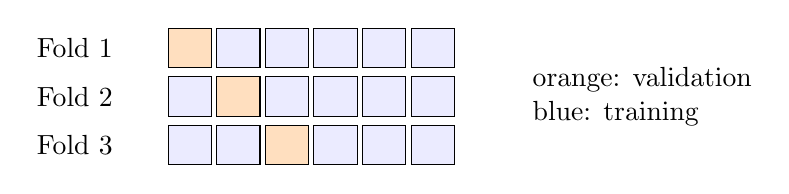
\begin{tikzpicture}[
  scale=.95,
  fold/.style={draw, minimum width=.55cm, minimum height=.5cm},
  val/.style={draw, fill=orange!25, minimum width=.55cm, minimum height=.5cm},
  train/.style={draw, fill=blue!8, minimum width=.55cm, minimum height=.5cm}
]
\foreach \r in {1,2,3} {
  \node[left] at (-.25,-.65*\r) {Fold \r};
  \foreach \c in {1,...,6} {
    \ifnum\c=\r
      \node[val] at (.65*\c,-.65*\r) {};
    \else
      \node[train] at (.65*\c,-.65*\r) {};
    \fi
  }
}
\node[align=left] at (6.7,-1.3) {orange: validation\\blue: training};
\end{tikzpicture}
\caption{In V-fold cross-validation, each fold is used once for validation.}
\label{fig:ch5-vfold}
\end{figure}

\subsection{Choosing the Number of Folds}

The number of folds controls a practical tradeoff.

With a larger $V$, each training set is closer in size to the full dataset. This can be
helpful in small samples or with flexible algorithms that need many observations to
train well. Leave-one-out cross-validation is the extreme case $V=n$.

With a smaller $V$, each validation fold is larger. This can make validation risk
estimates more stable, especially when outcomes are rare or highly skewed. Smaller
$V$ is also computationally cheaper because fewer models are fit.

Common choices include $V=5$ and $V=10$. The choice should be made before looking at
which algorithms win.

\subsection{Cross-Validated Risk as External-Data Mimicry}

The ideal way to evaluate a regression estimator would be to fit it in the study
sample and test it in a new independent sample from the same population. Such data
are rarely available. Cross-validation approximates this ideal by repeatedly creating
temporary training and validation samples from the observed data.

This matters for causal inference because nuisance functions are often selected before
being inserted into causal effect estimators. Cross-validated risk gives a pre-specified,
objective criterion for choosing among candidate outcome regressions or propensity
score models.

\begin{estimationbox}
V-fold cross-validation workflow:
\begin{enumerate}
\item Split the sample into $V$ folds.
\item For each candidate regression estimator and each fold, fit the estimator on the
training folds.
\item Predict on the held-out fold.
\item Compute validation loss.
\item Average validation loss over folds.
\item Prefer candidates with lower cross-validated risk.
\end{enumerate}
\end{estimationbox}

\lecture{5.5}{Candidate Estimator Selection}
\label{lec:5-5}

\subsection{Pre-Specifying the Candidate Library}

A candidate library is a set of regression algorithms chosen before looking at which
one gives the desired causal result. For outcome regression, the library might contain
linear regression, logistic regression, generalized additive models, random forests,
lasso, regression trees, splines, and neural networks. For propensity score estimation,
the same broad idea applies, but the outcome being predicted is treatment $A$ rather
than outcome $Y$.

\begin{definition}[Candidate library]
A candidate library is a pre-specified collection
\[
\mathcal L=\{\mathcal A_1,\ldots,\mathcal A_K\}
\]
of regression algorithms. When algorithm $\mathcal A_k$ is trained on the observed
data, it produces a fitted regression estimator $\Qbar_{n,k}$ or $g_{n,k}$.
\end{definition}

The library should be broad enough to include methods with different bias-variance
profiles. A useful library often contains both simple stable methods and flexible
adaptive methods. The simple methods protect against overfitting in small samples;
the flexible methods protect against bias when the true regression is complex.

\subsection{Comparing Regressions Using Cross-Validated Risk}

For each candidate algorithm $k$, compute its cross-validated risk:
\[
R_{CV,n}(\Qbar_{n,k})
=
\frac{1}{V}\sum_{v=1}^V
\frac{1}{|\mathcal V_v|}
\sum_{i\in\mathcal V_v}
L(\Qbar_{n,k,v})(W_i,A_i,Y_i),
\]
where $\Qbar_{n,k,v}$ is algorithm $k$ fit on the training data excluding validation
fold $\mathcal V_v$.

The candidate with the smallest cross-validated risk is selected:
\[
k_{CV}
=
\argmin_{k\in\{1,\ldots,K\}}
R_{CV,n}(\Qbar_{n,k}).
\]
The selected algorithm is then refit on the full dataset to produce the final nuisance
function estimate.

\subsection{Discrete Super Learner}

\begin{definition}[Discrete Super Learner]
The discrete Super Learner is the cross-validation selector that chooses the single
candidate algorithm with the lowest cross-validated risk and then refits that algorithm
on the full sample.
\end{definition}

The word ``discrete'' means that the final estimator is one member of the candidate
library, not a weighted combination. If the library contains $K$ algorithms, the
discrete Super Learner chooses one of those $K$ algorithms.

\begin{estimationbox}
Discrete Super Learner for an outcome regression:
\begin{enumerate}
\item Pre-specify candidate algorithms $\mathcal A_1,\ldots,\mathcal A_K$.
\item Choose a valid loss function for $\Qbar$, such as squared-error loss or
negative log-likelihood loss.
\item Compute cross-validated risk for each candidate.
\item Select the candidate with the smallest cross-validated risk.
\item Refit the selected candidate on the full sample.
\item Use the resulting $\Qbar_n$ inside the causal estimator.
\end{enumerate}
\end{estimationbox}

\subsection{Avoiding Post-Hoc Model Checking}

Traditional regression workflows often involve fitting a model, checking residual
plots or diagnostic tables, adding or removing terms, and refitting. This can be useful
for scientific exploration, but it creates problems for confirmatory estimation and
inference if the final model is chosen after seeing the data.

The issue is not that diagnostics are bad. The issue is that ordinary standard errors
and confidence intervals usually treat the final model as if it had been chosen in
advance. They do not account for the uncertainty introduced by trying many models
and selecting one.

Super Learning addresses this by moving model choice into a pre-specified algorithm.
If one would consider a main-terms model, an interaction model, a spline model, and a
random forest after inspecting diagnostics, those options can be placed in the library
in advance. Cross-validated risk then supplies the selection rule.

\begin{keyidea}
The analysis plan should specify the library, loss function, cross-validation scheme,
and selection rule before examining which candidate gives the most favorable causal
estimate.
\end{keyidea}

\subsection{Using Cross-Validation for Outcome Regression and Propensity Score Estimation}

The same framework applies to the two central nuisance functions:
\[
\Qbar(a,w)=\E(Y\given A=a,W=w),
\qquad
g_1(w)=\Prob(A=1\given W=w).
\]
For outcome regression, the validation loss compares predicted outcomes with
observed outcomes. For propensity score estimation, the validation loss compares
predicted treatment probabilities with observed treatment values.

For a binary treatment, a common propensity-score loss is the Bernoulli negative
log-likelihood:
\[
L(g_n)(w,a)
=
-a\log\{g_n(w)\}-(1-a)\log\{1-g_n(w)\}.
\]
This loss is minimized by the true conditional treatment probability
$\Prob(A=1\given W=w)$.

It is common for different algorithms to perform best for different nuisance
functions. A highly flexible method might predict the outcome well but estimate the
propensity score poorly, or vice versa. Therefore, the outcome regression library and
propensity score library should be evaluated separately, with losses appropriate to
each target.

\begin{implementationbox}
Conceptual R workflow:
\begin{lstlisting}[language=R]
# Outcome regression library:
# compare algorithms by cross-validated loss for predicting Y from A and W.

# Propensity score library:
# compare algorithms by cross-validated loss for predicting A from W.

# The selected outcome algorithm and selected propensity algorithm
# need not be the same.
\end{lstlisting}
\end{implementationbox}

\lecture{5.6}{Super Learner Ensembles}
\label{lec:5-6}

\subsection{Weighted Combinations of Estimators}

The discrete Super Learner chooses one candidate algorithm. But different algorithms
may capture different features of the data. A regression tree may capture threshold
effects, a generalized additive model may capture smooth nonlinearities, and a lasso
model may be stable in moderately high dimensions. Instead of choosing exactly one,
we can combine them.

Let $\Qbar_{n,1},\ldots,\Qbar_{n,K}$ be fitted candidate outcome regressions. A
weighted ensemble has the form
\[
\Qbar_{n,\omega}(a,w)
=
\sum_{k=1}^K \omega_k \Qbar_{n,k}(a,w),
\]
where $\omega=(\omega_1,\ldots,\omega_K)$ is a vector of weights.

\subsection{Convex Combinations}

Super Learner commonly uses convex combinations:
\[
\omega_k\ge 0,\qquad \sum_{k=1}^K\omega_k=1.
\]
The set of all such weights is the simplex
\[
\Delta_K=\left\{\omega\in\R^K:\omega_k\ge 0,\ \sum_{k=1}^K\omega_k=1\right\}.
\]

Convex combinations have a simple interpretation. If $\omega_3=0.70$ and
$\omega_5=0.30$, the ensemble prediction is 70\% from algorithm 3 and 30\% from
algorithm 5. Algorithms with weight zero do not contribute to the final prediction.

\begin{figure}[H]
\centering
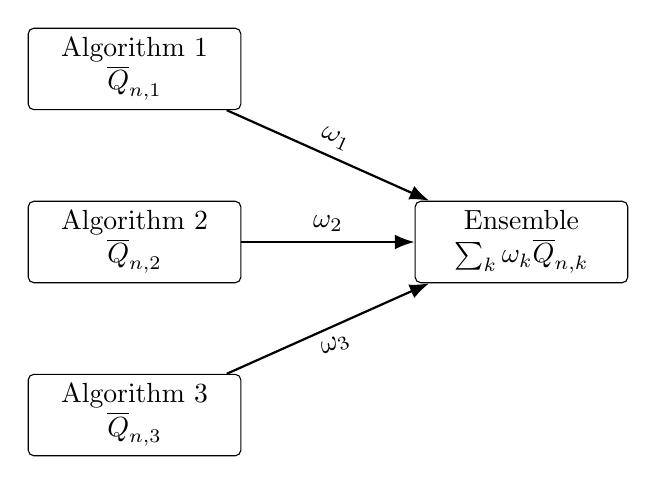
\begin{tikzpicture}[
  node distance=1.15cm,
  box/.style={draw, rounded corners=2pt, minimum width=2.7cm, minimum height=.75cm},
  arr/.style={-{Latex[length=2.5mm]}, thick}
]
\node[box] (a1) {Algorithm 1\\ $\Qbar_{n,1}$};
\node[box, below=of a1] (a2) {Algorithm 2\\ $\Qbar_{n,2}$};
\node[box, below=of a2] (a3) {Algorithm 3\\ $\Qbar_{n,3}$};
\node[box, right=2.2cm of a2] (ens) {Ensemble\\ $\sum_k\omega_k\Qbar_{n,k}$};
\draw[arr] (a1) -- node[above, sloped] {$\omega_1$} (ens);
\draw[arr] (a2) -- node[above] {$\omega_2$} (ens);
\draw[arr] (a3) -- node[below, sloped] {$\omega_3$} (ens);
\end{tikzpicture}
\caption{A Super Learner ensemble combines candidate predictions using learned weights.}
\label{fig:ch5-ensemble}
\end{figure}

\subsection{Choosing Weights by Cross-Validated Risk Minimization}

The Super Learner chooses $\omega$ to minimize cross-validated risk. For each fold
$v$, each candidate algorithm is trained on the training folds and predicts the
validation fold. For a proposed weight vector $\omega$, the ensemble prediction in
the validation fold is
\[
\Qbar_{n,\omega,v}(a,w)
=
\sum_{k=1}^K\omega_k\Qbar_{n,k,v}(a,w).
\]
The cross-validated risk of the ensemble is
\[
R_{CV,n}(\omega)
=
\frac{1}{V}\sum_{v=1}^V
\frac{1}{|\mathcal V_v|}
\sum_{i\in\mathcal V_v}
L(\Qbar_{n,\omega,v})(W_i,A_i,Y_i).
\]
The selected weights are
\[
\omega_{CV}
=
\argmin_{\omega\in\Delta_K}R_{CV,n}(\omega).
\]
After the weights are selected, each candidate algorithm is refit on the full dataset,
and the final Super Learner is
\[
\Qbar_{n,SL}(a,w)
=
\sum_{k=1}^K\omega_{CV,k}\Qbar_{n,k}^{\mathrm{full}}(a,w).
\]

\subsection{Oracle Inequalities}

The theoretical appeal of Super Learner comes from oracle inequalities. An oracle is
an imaginary procedure that knows the true risks of all candidates and chooses the
best one. The analyst cannot implement the oracle because true risk depends on the
unknown data-generating distribution.

An oracle inequality states, under regularity conditions, that the cross-validation
selector or ensemble performs nearly as well as the oracle, up to a term that becomes
small as sample size grows. A simplified version of the message is
\[
\text{risk of Super Learner}
\le
\text{risk of oracle choice}
+
\text{small remainder}.
\]
The remainder depends on sample size and on the size of the candidate library. This
supports the practical strategy of including a diverse pre-specified library rather than
trying to guess a single correct model.

\begin{keyidea}
The oracle is the best procedure in the chosen library for the data-generating
distribution. Super Learner uses cross-validation to approximate that oracle without
knowing the truth.
\end{keyidea}

\subsection{Model Stacking}

Combining candidate predictions is often called stacking. The idea is to treat the
out-of-fold predictions from the candidate algorithms as inputs to a second-stage
learner, sometimes called the metalearner. In the convex Super Learner, the
metalearner is a constrained regression that finds nonnegative weights summing to
one.

Stacking differs from ordinary model averaging based on subjective preference. The
weights are chosen to minimize a pre-specified cross-validated loss. This makes the
ensemble a fully specified estimator rather than a post-hoc compromise among models.

\subsection{Super Learner vs Single Best Algorithm}

The discrete Super Learner is guaranteed to choose one candidate. The ensemble Super
Learner can choose one candidate by putting all weight on it, but it can also combine
multiple candidates when that lowers cross-validated risk. Thus the ensemble contains
the discrete choice as a special case.

\begin{estimationbox}
Ensemble Super Learner workflow:
\begin{enumerate}
\item Pre-specify candidate algorithms and a valid loss function.
\item Generate out-of-fold predictions for every algorithm.
\item Choose convex weights minimizing cross-validated risk.
\item Refit all candidate algorithms on the full dataset.
\item Combine full-data predictions using the selected weights.
\item Use the resulting nuisance function estimate inside the causal estimator.
\end{enumerate}
\end{estimationbox}

\lecture{5.7}{Practical Interpretation of Super Learner Results}
\label{lec:5-7}

\subsection{Candidate Algorithms}

A Super Learner analysis should report the candidate library. The library is part of
the estimator. Two analyses with different libraries are using different statistical
procedures, even if both are called Super Learner.

Common candidate algorithms include:
\begin{itemize}
\item generalized linear models;
\item models with interactions or polynomial terms;
\item penalized regressions such as lasso and ridge;
\item generalized additive models;
\item multivariate adaptive regression splines;
\item regression trees and random forests;
\item gradient boosting;
\item Bayesian additive regression trees;
\item support vector machines;
\item neural networks;
\item simple empirical or intercept-only benchmarks.
\end{itemize}

The library should include algorithms with different levels of flexibility. It is often
useful to include simple benchmark models because they can perform well when the
sample is small or the signal is simple.

\subsection{Cross-Validated Risk Tables}

Super Learner output often includes a table of cross-validated risks. For squared-error
loss, lower risk means lower estimated out-of-sample mean squared error. For negative
log-likelihood loss, lower risk means better predicted probabilities.

A risk table might have the following conceptual form:
\[
\begin{array}{lcc}
\toprule
\text{Algorithm} & \text{CV risk for }\Qbar & \text{CV risk for }g\\
\midrule
\text{GLM} & 1.000 & 1.000\\
\text{GAM} & 0.994 & 0.987\\
\text{Random forest} & 0.997 & 0.989\\
\text{BART} & 0.988 & 4.462\\
\text{Super Learner} & 0.986 & 0.983\\
\bottomrule
\end{array}
\]
Risks are sometimes reported relative to a reference method, such as GLM. A relative
risk below 1 means the algorithm had lower cross-validated risk than the reference.
A relative risk above 1 means it performed worse by the chosen loss.

\subsection{Super Learner Weights}

The ensemble weights describe how the final prediction function is assembled:
\[
\Qbar_{n,SL}(a,w)=\sum_{k=1}^K\omega_k\Qbar_{n,k}(a,w).
\]
A large weight means that an algorithm contributes substantially to the final ensemble
prediction. A zero weight means that the algorithm did not improve the ensemble risk
given the other algorithms in the library.

Weights should not be interpreted as posterior probabilities that a model is true. A
Super Learner library is not a list of mutually exclusive scientific models. It is a
collection of prediction algorithms. The weights are chosen for predictive performance
under a loss function, not for causal interpretation.

\subsection{Why Zero Weights Are Common}

Zero weights are common because many algorithms make similar predictions. If two
algorithms are highly correlated, the ensemble may need only one of them. An
algorithm can also receive zero weight because it predicts poorly, because it is
redundant with better algorithms, or because adding it would increase validation risk.

Zero weight does not necessarily mean an algorithm is useless in all datasets. It means
that, in this dataset and this library, the cross-validated metalearner did not find it
helpful for reducing the chosen risk.

\begin{keyidea}
Super Learner weights are performance weights, not truth weights. They summarize
how candidate predictions were combined to minimize cross-validated loss.
\end{keyidea}

\subsection{Outcome Regression vs Propensity Score Performance}

The same algorithm can perform differently for $\Qbar$ and $g$. The outcome
regression predicts $Y$ from $(A,W)$, while the propensity score predicts $A$ from
$W$. These are different statistical tasks.

For example, a flexible tree-based method might capture nonlinear outcome patterns
well but produce unstable propensity scores near zero or one. A generalized additive
model might predict treatment assignment well because the treatment mechanism is
smooth, while offering little improvement for a noisy outcome.

This distinction is important for causal estimators. In g-computation, the outcome
regression is the central nuisance function. In IPTW, the propensity score is central.
In doubly robust estimators introduced later, both nuisance functions matter, and their
estimation quality can affect bias, variance, and confidence interval behavior.

\subsection{Reporting Model Libraries and Sensitivity Analyses}

Transparent reporting should include:
\begin{itemize}
\item the candidate algorithms;
\item important tuning parameter grids;
\item the loss function;
\item the number of cross-validation folds;
\item whether candidates used screening or preprocessing;
\item the cross-validated risks;
\item the selected discrete learner or ensemble weights;
\item any convergence failures or algorithms removed before analysis.
\end{itemize}

Sensitivity analyses are useful because Super Learner performance depends on the
library. A narrow library cannot choose a method that was not included. Analysts
should examine whether conclusions change when the library is expanded, when
highly unstable algorithms are removed, or when alternative reasonable losses are
used.

\begin{implementationbox}
Practical reporting template:
\begin{lstlisting}
Outcome regression:
  Loss: squared-error or negative log-likelihood
  Folds: V-fold cross-validation
  Library: GLM, GAM, lasso, random forest, ...
  Selected/weighted algorithms: report CV risks and weights

Propensity score:
  Loss: Bernoulli negative log-likelihood
  Folds: V-fold cross-validation
  Library: GLM, GAM, lasso, random forest, ...
  Diagnostics: predicted probabilities and weight summaries
\end{lstlisting}
\end{implementationbox}

\begin{estimationbox}
When Super Learner is used inside a causal analysis, it should be described as part
of the estimator of the causal parameter. Report the causal assumptions separately
from the regression performance. Good cross-validated prediction does not verify
exchangeability, consistency, or positivity.
\end{estimationbox}


\chapterheading{6}{Super Learning Lab}
\lecture{6.1}{Software Setup and Simulated Data}
\label{lec:6-1}

\subsection{Required R Packages}

This chapter is a computational lab for the ideas developed in Chapter 5. The goal is
to see how cross-validated risk minimization and Super Learner ensembles are
implemented in practice. The examples use simulated data so that the true treatment
mechanism and true outcome regression are known.

The main package is \texttt{SuperLearner}. Several other packages are often useful
because they supply candidate algorithms or optimization routines. A typical setup is:

\begin{implementationbox}
\begin{lstlisting}[language=R]
pkgs <- c("SuperLearner", "quadprog", "nloptr", "MASS",
          "ggplot2", "nnls")

installed_packages <- row.names(installed.packages())

for (p in pkgs) {
  if (!(p %in% installed_packages)) {
    install.packages(p)
  }
  library(p, character.only = TRUE)
}
\end{lstlisting}
\end{implementationbox}

The packages \texttt{quadprog}, \texttt{nloptr}, and \texttt{nnls} are optimization
tools used by some Super Learner metalearners. The package \texttt{MASS} supplies
regression utilities, and \texttt{ggplot2} is useful for plotting. Additional candidate
algorithms may require additional packages.

\subsection{Loading \texttt{SuperLearner}}

After installation, the package can be loaded with:

\begin{implementationbox}
\begin{lstlisting}[language=R]
library(SuperLearner)
\end{lstlisting}
\end{implementationbox}

The package provides two kinds of functions:
\begin{itemize}
\item user-facing functions such as \texttt{SuperLearner()} and
\texttt{CV.SuperLearner()};
\item wrapper functions, for example \texttt{SL.glm} and \texttt{SL.mean};
these tell the package how to fit candidate algorithms.
\end{itemize}

To view available built-in learners and screeners:

\begin{implementationbox}
\begin{lstlisting}[language=R]
listWrappers(what = "SL")
listWrappers(what = "screen")
\end{lstlisting}
\end{implementationbox}

\subsection{Simulated Covariates}

We simulate $n$ independent observations with two covariates:
\[
W_1\sim N(0,1), \qquad W_2\sim \operatorname{Uniform}(0,1).
\]
These covariates are deliberately simple, but they are rich enough to illustrate
interactions and nonlinear candidate regressions.

\begin{implementationbox}
\begin{lstlisting}[language=R]
set.seed(212)

n <- 500
W1 <- rnorm(n = n)
W2 <- runif(n = n)
\end{lstlisting}
\end{implementationbox}

\subsection{Simulated Treatment Mechanism}

Treatment is binary. The true propensity score is
\[
g_1(W)=\Prob(A=1\given W)
=
\expit(-1+W_1-W_2+2W_1W_2).
\]
This treatment mechanism includes an interaction between $W_1$ and $W_2$. A main
terms logistic regression for $A$ on $W_1$ and $W_2$ is therefore misspecified.

\begin{implementationbox}
\begin{lstlisting}[language=R]
g1W <- plogis(-1 + W1 - W2 + 2 * W1 * W2)
A <- rbinom(n = n, size = 1, prob = g1W)
\end{lstlisting}
\end{implementationbox}

\begin{figure}[H]
\centering
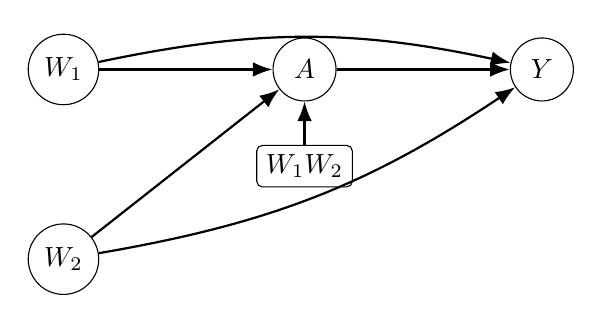
\begin{tikzpicture}[
  node distance=1.5cm,
  var/.style={draw, circle, minimum size=.8cm},
  arr/.style={-{Latex[length=2.5mm]}, thick}
]
\node[var] (W1) {$W_1$};
\node[var, below=of W1] (W2) {$W_2$};
\node[var, right=2.2cm of W1] (A) {$A$};
\node[var, right=2.2cm of A] (Y) {$Y$};
\draw[arr] (W1) -- (A);
\draw[arr] (W2) -- (A);
\draw[arr] (W1) to[bend left=12] (Y);
\draw[arr] (W2) to[bend right=12] (Y);
\draw[arr] (A) -- (Y);
\node[draw, rounded corners=2pt, below=.55cm of A] (int) {$W_1W_2$};
\draw[arr] (int) -- (A);
\end{tikzpicture}
\caption{The simulated data have covariate-dependent treatment and outcome mechanisms.}
\label{fig:ch6-sim-dag}
\end{figure}

\subsection{Simulated Outcome Regression}

The true outcome regression is linear:
\[
\Qbar(A,W)=\E(Y\given A,W)=W_1-W_2+A.
\]
The observed outcome is generated by adding independent normal noise:
\[
Y=\Qbar(A,W)+\varepsilon,\qquad \varepsilon\sim N(0,1).
\]

\begin{implementationbox}
\begin{lstlisting}[language=R]
QAW <- W1 - W2 + A
Y <- QAW + rnorm(n = n)

full_data <- data.frame(W1 = W1, W2 = W2, A = A, Y = Y)
\end{lstlisting}
\end{implementationbox}

Because the true $\Qbar$ is known, we can check whether flexible methods behave
sensibly. However, in real applications the true regression function is unknown. The
point of the lab is to practice methods that are useful precisely because the truth is
not known.

\subsection{Reproducibility with Seeds}

Simulation, cross-validation splits, and some machine learning algorithms involve
randomness. A random seed makes the analysis reproducible:

\begin{implementationbox}
\begin{lstlisting}[language=R]
set.seed(212)
\end{lstlisting}
\end{implementationbox}

Using a seed does not make the result less random in a statistical sense. It fixes the
particular random draw so that another analyst running the same code obtains the
same simulated data, folds, and fitted results.

\begin{keyidea}
In a lab setting, seeds make examples reproducible. In a scientific analysis, they also
make computational results auditable: the same data and same code should lead to the
same reported estimates.
\end{keyidea}

\lecture{6.2}{Manual Cross-Validation}
\label{lec:6-2}

\subsection{Full-Data Risk vs Cross-Validated Risk}

Before calling \texttt{SuperLearner()}, it is useful to implement cross-validation by
hand. This makes clear what the package automates.

Consider two candidate estimators for the outcome regression $\Qbar(A,W)$:
\[
\Qbar_{n,1}: \text{ main-terms linear regression},
\]
\[
\Qbar_{n,2}: \text{ a more flexible regression with quadratic and interaction terms}.
\]
The mean squared-error risk of a fitted estimator $Q$ is
\[
R(Q)=\E\left[\{Y-Q(A,W)\}^2\right].
\]
The naive full-data empirical risk is
\[
R_n(Q_n)=\frac{1}{n}\sum_{i=1}^n\{Y_i-Q_n(A_i,W_i)\}^2.
\]
This quantity can be too optimistic because the same observations are used both to fit
the regression and to evaluate its error.

\begin{implementationbox}
\begin{lstlisting}[language=R]
Q1_fit <- glm(Y ~ W1 + W2 + A, data = full_data)
Q1n <- as.numeric(predict(Q1_fit))
risk_Q1_full <- mean((Y - Q1n)^2)

Q2_fit <- glm(Y ~ I(W1^2) + I(W2^2) + W1 * W2 + W1 * A + W2 * A,
              data = full_data)
Q2n <- as.numeric(predict(Q2_fit))
risk_Q2_full <- mean((Y - Q2n)^2)
\end{lstlisting}
\end{implementationbox}

\subsection{Two-Fold Splitting}

Two-fold cross-validation splits the data into two validation sets. Each fold is used
once for validation and once as part of the training data. With two folds, the training
set for fold 1 is fold 2, and the training set for fold 2 is fold 1.

\begin{implementationbox}
\begin{lstlisting}[language=R]
split <- c(rep(1, n / 2), rep(2, n / 2))

split1 <- subset(full_data, split == 1)
split2 <- subset(full_data, split == 2)
\end{lstlisting}
\end{implementationbox}

In real analyses, folds are usually randomized rather than assigning the first half to
one fold and the second half to another. For teaching, a deterministic split makes the
logic easier to see.

\subsection{Training Regressions}

For $\Qbar_{n,1}$, fit the main-terms model on split 1 and validate on split 2:

\begin{implementationbox}
\begin{lstlisting}[language=R]
Q1_fit_split1 <- glm(Y ~ W1 + W2 + A, data = split1)
Q1n_split2 <- predict(Q1_fit_split1, newdata = split2)
risk_Q1_split2 <- mean((split2$Y - Q1n_split2)^2)
\end{lstlisting}
\end{implementationbox}

Then reverse the roles:

\begin{implementationbox}
\begin{lstlisting}[language=R]
Q1_fit_split2 <- glm(Y ~ W1 + W2 + A, data = split2)
Q1n_split1 <- predict(Q1_fit_split2, newdata = split1)
risk_Q1_split1 <- mean((split1$Y - Q1n_split1)^2)
\end{lstlisting}
\end{implementationbox}

\subsection{Validation Predictions}

The essential rule is that validation predictions must be made using a model that did
not train on the validation observations. For observation $i$ in validation fold $v$,
the prediction has the form
\[
\Qbar_{n,v}(A_i,W_i),
\]
where $\Qbar_{n,v}$ was fit using the training observations outside fold $v$.

\begin{figure}[H]
\centering
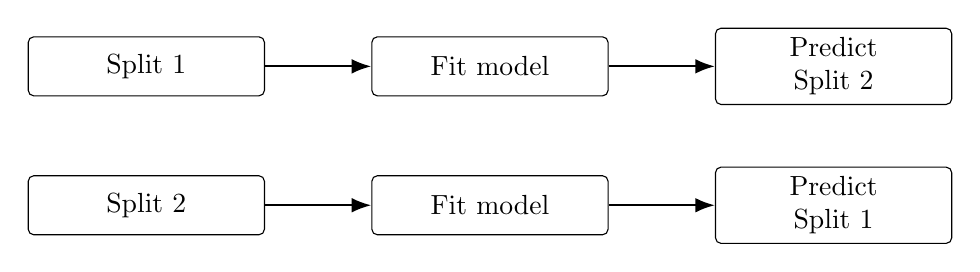
\begin{tikzpicture}[
  node distance=1.35cm,
  box/.style={draw, rounded corners=2pt, minimum width=3.0cm, minimum height=.75cm},
  arr/.style={-{Latex[length=2.5mm]}, thick}
]
\node[box] (s1) {Split 1};
\node[box, right=of s1] (fit1) {Fit model};
\node[box, right=of fit1] (pred2) {Predict\\ Split 2};
\draw[arr] (s1) -- (fit1);
\draw[arr] (fit1) -- (pred2);
\node[box, below=1cm of s1] (s2) {Split 2};
\node[box, right=of s2] (fit2) {Fit model};
\node[box, right=of fit2] (pred1) {Predict\\ Split 1};
\draw[arr] (s2) -- (fit2);
\draw[arr] (fit2) -- (pred1);
\end{tikzpicture}
\caption{Two-fold cross-validation swaps training and validation roles.}
\label{fig:ch6-twofold}
\end{figure}

\subsection{Mean Squared-Error Risk}

The two-fold cross-validated risk estimate is the average of the two fold-specific
validation risks:
\[
R_{CV,n}(\Qbar_{n,1})
=
\frac{1}{2}\left\{
R_{n,1}(\Qbar_{n,1,2})+
R_{n,2}(\Qbar_{n,1,1})
\right\}.
\]
In code:

\begin{implementationbox}
\begin{lstlisting}[language=R]
cv_risk_Q1 <- (risk_Q1_split1 + risk_Q1_split2) / 2
\end{lstlisting}
\end{implementationbox}

For the flexible model, repeat the same process:

\begin{implementationbox}
\begin{lstlisting}[language=R]
Q2_formula <- Y ~ I(W1^2) + I(W2^2) + W1 * W2 + W1 * A + W2 * A

Q2_fit_split1 <- glm(Q2_formula, data = split1)
Q2n_split2 <- predict(Q2_fit_split1, newdata = split2)
risk_Q2_split2 <- mean((split2$Y - Q2n_split2)^2)

Q2_fit_split2 <- glm(Q2_formula, data = split2)
Q2n_split1 <- predict(Q2_fit_split2, newdata = split1)
risk_Q2_split1 <- mean((split1$Y - Q2n_split1)^2)

cv_risk_Q2 <- (risk_Q2_split1 + risk_Q2_split2) / 2
\end{lstlisting}
\end{implementationbox}

\subsection{Comparing Simple and Flexible Regressions}

The candidate with lower cross-validated risk has better estimated out-of-sample
prediction performance under the chosen loss. A flexible model can have lower
training risk but higher cross-validated risk if it overfits. Conversely, a simple model
can win when the true signal is simple or when the sample size is limited.

\begin{keyidea}
Cross-validation evaluates how well a regression predicts observations it did not use
for training. This is why cross-validated risk is a better guide for selecting nuisance
regressions than full-data training error.
\end{keyidea}

\lecture{6.3}{Manual Ensemble Construction}
\label{lec:6-3}

\subsection{Ensemble Prediction Functions}

An ensemble combines predictions from multiple fitted regressions. With two
candidate outcome regressions $\Qbar_{n,1}$ and $\Qbar_{n,2}$, a convex ensemble is
\[
\Qbar_{n,\omega}(a,w)
=
\omega \Qbar_{n,1}(a,w)+(1-\omega)\Qbar_{n,2}(a,w),
\qquad 0\le \omega\le 1.
\]
The weight $\omega$ controls how much the ensemble uses the first candidate. If
$\omega=1$, the ensemble is $\Qbar_{n,1}$. If $\omega=0$, the ensemble is
$\Qbar_{n,2}$.

\subsection{Weighted Averages of Candidate Predictions}

The following function takes two fitted \texttt{glm} objects, obtains predictions from
each, and returns their weighted average:

\begin{implementationbox}
\begin{lstlisting}[language=R]
ensemble_predict <- function(Q1_fit, Q2_fit, newdata,
                             Q1_weight, Q2_weight = 1 - Q1_weight) {
  stopifnot(abs(1 - Q1_weight - Q2_weight) < 1e-5)

  Q1n <- predict(Q1_fit, newdata = newdata)
  Q2n <- predict(Q2_fit, newdata = newdata)

  ensemble_prediction <- Q1_weight * Q1n + Q2_weight * Q2n
  as.numeric(ensemble_prediction)
}
\end{lstlisting}
\end{implementationbox}

For one new observation, this function computes
\[
\omega \hat y_1+(1-\omega)\hat y_2.
\]
For many observations, it computes the same formula row by row.

\subsection{Weight Grids}

With two candidates, a simple way to search over possible ensembles is to create a
grid of weights:

\begin{implementationbox}
\begin{lstlisting}[language=R]
weight_sequence <- seq(from = 0, to = 1, length.out = 500)
\end{lstlisting}
\end{implementationbox}

Each value in \texttt{weight\_sequence} defines a different candidate ensemble.
The grid is only an approximation to the continuum $[0,1]$, but it is sufficient for
illustrating the idea. With many candidates, the weight vector lies in a higher
dimensional simplex, and numerical optimization methods are used instead of a simple
grid.

\begin{figure}[H]
\centering
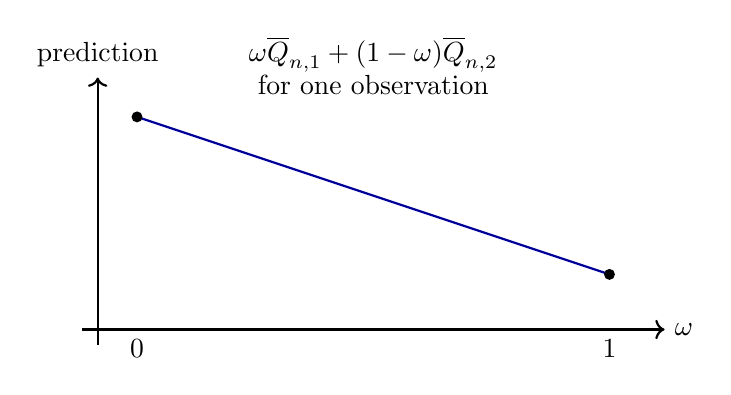
\begin{tikzpicture}[
  axis/.style={->, thick},
  pt/.style={circle, fill=black, inner sep=1.4pt}
]
\draw[axis] (-.2,0) -- (7.2,0) node[right] {$\omega$};
\draw[axis] (0,-.2) -- (0,3.2) node[above] {prediction};
\draw[thick, blue!60!black] (0.5,2.7) -- (6.5,.7);
\node[pt] at (.5,2.7) {};
\node[pt] at (6.5,.7) {};
\node[below] at (.5,0) {$0$};
\node[below] at (6.5,0) {$1$};
\node[align=center] at (3.5,3.35) {$\omega \Qbar_{n,1}+(1-\omega)\Qbar_{n,2}$\\for one observation};
\end{tikzpicture}
\caption{With two learners, ensemble predictions vary linearly with the weight.}
\label{fig:ch6-weight-path}
\end{figure}

\subsection{Cross-Validated Risk Across Weights}

For each weight, compute out-of-fold ensemble predictions and evaluate mean
squared-error loss. For a fixed $\omega$, the two-fold estimate is
\[
R_{CV,n}(\omega)
=
\frac{1}{2}
\left[
\frac{1}{n_1}\sum_{i\in \mathcal V_1}
\{Y_i-\Qbar_{n,\omega,2}(A_i,W_i)\}^2
+
\frac{1}{n_2}\sum_{i\in \mathcal V_2}
\{Y_i-\Qbar_{n,\omega,1}(A_i,W_i)\}^2
\right],
\]
where $\Qbar_{n,\omega,2}$ is the ensemble built from models trained in split 2 and
validated in split 1, and $\Qbar_{n,\omega,1}$ is the analogous ensemble trained in
split 1 and validated in split 2.

\begin{implementationbox}
\begin{lstlisting}[language=R]
cv_risks <- rep(NA_real_, length(weight_sequence))

for (i in seq_along(weight_sequence)) {
  w <- weight_sequence[i]

  pred_split2 <- ensemble_predict(Q1_fit_split1, Q2_fit_split1,
                                  newdata = split2,
                                  Q1_weight = w)
  risk_split2 <- mean((split2$Y - pred_split2)^2)

  pred_split1 <- ensemble_predict(Q1_fit_split2, Q2_fit_split2,
                                  newdata = split1,
                                  Q1_weight = w)
  risk_split1 <- mean((split1$Y - pred_split1)^2)

  cv_risks[i] <- (risk_split1 + risk_split2) / 2
}
\end{lstlisting}
\end{implementationbox}

\subsection{Selecting Optimal Ensemble Weights}

The Super Learner weight is the value with the smallest cross-validated risk:
\[
\omega_{CV}=\argmin_{\omega\in[0,1]}R_{CV,n}(\omega).
\]
On a grid, this is computed by:

\begin{implementationbox}
\begin{lstlisting}[language=R]
min_idx <- which.min(cv_risks)
omega_hat <- weight_sequence[min_idx]
min_cv_risk <- cv_risks[min_idx]
\end{lstlisting}
\end{implementationbox}

After the weight is selected, the candidate regressions are typically refit on the full
dataset. The final ensemble prediction function is
\[
\Qbar_{n,SL}(a,w)
=
\omega_{CV}\Qbar_{n,1}^{\mathrm{full}}(a,w)
+
(1-\omega_{CV})\Qbar_{n,2}^{\mathrm{full}}(a,w).
\]

\begin{keyidea}
Manual ensemble construction has two layers of learning. First, each candidate
regression learns from training data. Second, the ensemble learns weights by comparing
out-of-fold predictions.
\end{keyidea}

\begin{estimationbox}
When there are more than two candidates, Super Learner chooses weights
$\omega_1,\ldots,\omega_K$ satisfying $\omega_k\ge 0$ and $\sum_k\omega_k=1$.
Specialized optimization routines find the cross-validated risk minimizer over this
simplex more efficiently than a grid search.
\end{estimationbox}

\lecture{6.4}{Basic Calls to \texttt{SuperLearner}}
\label{lec:6-4}

\subsection{Main Arguments: \texttt{Y}, \texttt{X}, \texttt{SL.library}, \texttt{family}, \texttt{method}, \texttt{cvControl}}

The function \texttt{SuperLearner()} automates the cross-validation and ensemble
construction described in the previous lectures. Its most important arguments are:
\begin{itemize}
\item \texttt{Y}: the outcome to be predicted;
\item \texttt{X}: a data frame or matrix of predictors;
\item \texttt{SL.library}: candidate algorithms;
\item \texttt{family}: the outcome family, commonly \texttt{gaussian()} or
\texttt{binomial()};
\item \texttt{method}: the metalearner and loss used to choose weights;
\item \texttt{cvControl}: options controlling the internal cross-validation.
\end{itemize}

For outcome regression, \texttt{Y} is the observed outcome and \texttt{X} contains
$(A,W)$. For propensity score estimation, \texttt{Y} is the treatment $A$ and
\texttt{X} contains $W$.

\begin{implementationbox}
\begin{lstlisting}[language=R]
set.seed(123)

sl_fit1 <- SuperLearner(
  Y = Y,
  X = data.frame(W1 = W1, W2 = W2, A = A),
  SL.library = c("SL.glm", "SL.mean"),
  family = gaussian(),
  method = "method.CC_LS",
  cvControl = list(V = 2),
  verbose = FALSE
)
\end{lstlisting}
\end{implementationbox}

\subsection{Continuous vs Binary Outcomes}

For a continuous outcome regression, use \texttt{family = gaussian()} and a loss such
as squared-error loss. A common metalearner is \texttt{method.CC\_LS}, a convex
combination chosen to minimize least-squares loss.

For a binary outcome or binary treatment mechanism, use \texttt{family = binomial()}.
For predicted probabilities, a natural loss is negative log-likelihood. A useful
metalearner is \texttt{method.CC\_nloglik}.

\begin{implementationbox}
\begin{lstlisting}[language=R]
# Outcome regression for continuous Y
fit_Q <- SuperLearner(Y = Y,
                      X = data.frame(A = A, W1 = W1, W2 = W2),
                      SL.library = c("SL.glm", "SL.mean"),
                      family = gaussian(),
                      method = "method.CC_LS")

# Propensity score for binary A
fit_g <- SuperLearner(Y = A,
                      X = data.frame(W1 = W1, W2 = W2),
                      SL.library = c("SL.glm", "SL.mean"),
                      family = binomial(),
                      method = "method.CC_nloglik")
\end{lstlisting}
\end{implementationbox}

\subsection{Interpreting Printed Output}

Printing a \texttt{SuperLearner} object shows the call, the cross-validated risk of
each candidate, and the final ensemble coefficients. A typical table has columns:
\[
\text{Risk},\qquad \text{Coef}.
\]
The risk column describes candidate performance under the chosen cross-validated
loss. The coefficient column gives the ensemble weight assigned to each candidate.

\subsection{Risk}

The reported risk is not the full-data training error. It is an internal
cross-validated risk estimate for each candidate algorithm. For Gaussian outcomes
with \texttt{method.CC\_LS}, this risk is mean squared prediction error. For binomial
outcomes with \texttt{method.CC\_nloglik}, it is negative log-likelihood risk.

Risk values are comparable only when they use the same outcome and same loss. A
mean squared-error risk for $Y$ should not be numerically compared with a
negative-log-likelihood risk for $A$.

\subsection{Coefficients}

The coefficients are the estimated ensemble weights. If a candidate has coefficient
zero, it does not contribute to the final Super Learner prediction. This does not mean
the candidate is scientifically impossible or universally poor; it means that, given the
other candidates and the selected loss, the metalearner did not need that candidate to
reduce cross-validated risk.

\begin{keyidea}
The risk table scores individual algorithms. The coefficients describe the ensemble.
An algorithm can have mediocre individual risk but still receive weight if its
predictions complement the predictions of other learners.
\end{keyidea}

\subsection{Super Learner Predictions}

The object returned by \texttt{SuperLearner()} contains fitted predictions for the
observed rows:

\begin{implementationbox}
\begin{lstlisting}[language=R]
head(sl_fit1$SL.predict)
\end{lstlisting}
\end{implementationbox}

Predictions for new observations are obtained with \texttt{predict()}:

\begin{implementationbox}
\begin{lstlisting}[language=R]
new_obs <- data.frame(A = 1, W1 = 0, W2 = 0)

new_predictions <- predict(sl_fit1, newdata = new_obs)
new_predictions$pred
\end{lstlisting}
\end{implementationbox}

The returned \texttt{pred} component is the ensemble prediction.

\subsection{Library Predictions}

The same prediction call also returns predictions from each library member:

\begin{implementationbox}
\begin{lstlisting}[language=R]
new_predictions$library.predict
\end{lstlisting}
\end{implementationbox}

Inside the fitted object, useful components include:
\begin{itemize}
\item \texttt{SL.predict}: Super Learner predictions in the original data;
\item \texttt{library.predict}: full-data predictions from each candidate;
\item \texttt{coef}: ensemble weights;
\item \texttt{cvRisk}: internal cross-validated risk estimates;
\item \texttt{fitLibrary}: fitted candidate algorithms;
\item \texttt{validRows}: validation fold membership.
\end{itemize}

\begin{estimationbox}
For causal estimation, the fitted Super Learner is still a nuisance-function estimator.
To use it in g-computation, predict $\Qbar_n(1,W_i)$ and $\Qbar_n(0,W_i)$ using
treatment-specific prediction datasets. To use it for IPTW, estimate $g_{n,1}(W_i)$
and form inverse probability weights.
\end{estimationbox}

\lecture{6.5}{Writing Custom SuperLearner Wrappers}
\label{lec:6-5}

\subsection{Wrapper Function Structure}

A Super Learner wrapper is an R function that tells \texttt{SuperLearner()} how to fit
a candidate algorithm and how to generate predictions during cross-validation. Built-in
wrappers such as \texttt{SL.glm} follow the same structure custom wrappers must
follow.

The wrapper must return a list with two named components:
\[
\texttt{pred},\qquad \texttt{fit}.
\]
The \texttt{pred} component contains predictions on \texttt{newX}. The \texttt{fit}
component stores the fitted object or any information needed for later prediction.

\subsection{Required Inputs}

A standard wrapper has the form:

\begin{implementationbox}
\begin{lstlisting}[language=R]
SL.myalgorithm <- function(Y, X, newX, family, obsWeights, ...) {
  # fit model using Y and X
  # predict on newX
  # return list(pred = pred, fit = fit)
}
\end{lstlisting}
\end{implementationbox}

The key inputs are:
\begin{itemize}
\item \texttt{Y}: training outcomes;
\item \texttt{X}: training predictors;
\item \texttt{newX}: validation or prediction predictors;
\item \texttt{family}: outcome family;
\item \texttt{obsWeights}: observation weights, if supplied;
\item \texttt{...}: additional arguments passed by the package.
\end{itemize}

The \texttt{...} argument is important. It allows the wrapper to ignore arguments it
does not use without failing.

\subsection{Returning \texttt{pred} and \texttt{fit}}

The \texttt{pred} vector must have length \texttt{nrow(newX)}. The \texttt{fit} object
can be any list, but it should contain everything needed for future calls to
\texttt{predict()}.

\begin{implementationbox}
\begin{lstlisting}[language=R]
out <- list(pred = pred, fit = fit)
return(out)
\end{lstlisting}
\end{implementationbox}

It is useful to assign a class to the \texttt{fit} object:

\begin{implementationbox}
\begin{lstlisting}[language=R]
class(out$fit) <- "SL.myalgorithm"
\end{lstlisting}
\end{implementationbox}

The class allows R to dispatch to a custom prediction method later.

\subsection{Writing Prediction Methods}

When \texttt{predict()} is called on a Super Learner object containing a custom wrapper,
R must know how to predict from the custom fitted object. If the class is
\texttt{"SL.myalgorithm"}, R looks for a function named
\texttt{predict.SL.myalgorithm()}.

\begin{implementationbox}
\begin{lstlisting}[language=R]
predict.SL.myalgorithm <- function(object, newdata, ...) {
  pred <- predict(object$fitted_model, newdata = newdata, type = "response")
  return(pred)
}
\end{lstlisting}
\end{implementationbox}

The exact prediction call depends on the object stored inside \texttt{fit}. If
\texttt{fit} stores a \texttt{glm}, use \texttt{predict.glm}. If it stores a random
forest, use the prediction method for that random forest object.

\subsection{Custom Quadratic GLM Wrapper}

The following wrapper fits a linear regression with quadratic terms in $W_1$ and
$W_2$:

\begin{implementationbox}
\begin{lstlisting}[language=R]
SL.quadglm <- function(Y, X, newX, family, obsWeights, ...) {
  X <- as.data.frame(X)
  newX <- as.data.frame(newX)

  fit_glm <- glm(Y ~ W1 + I(W1^2) + W2 + I(W2^2) + A,
                 data = X,
                 family = family,
                 weights = obsWeights)

  pred <- predict(fit_glm, newdata = newX, type = "response")

  fit <- list(fitted_model = fit_glm)
  class(fit) <- "SL.quadglm"

  list(pred = pred, fit = fit)
}

predict.SL.quadglm <- function(object, newdata, ...) {
  predict(object$fitted_model, newdata = as.data.frame(newdata),
          type = "response")
}
\end{lstlisting}
\end{implementationbox}

This wrapper assumes the columns \texttt{W1}, \texttt{W2}, and \texttt{A} exist in
\texttt{X}. If those names are absent, the wrapper will fail. Custom wrappers should
therefore be written with clear expectations about input variable names.

\subsection{Custom Propensity Score Wrapper}

For the simulated data, the true propensity score has a $W_1W_2$ interaction. A custom
wrapper can fit that logistic regression:

\begin{implementationbox}
\begin{lstlisting}[language=R]
SL.truepropensity <- function(Y, X, newX, family, obsWeights, ...) {
  X <- as.data.frame(X)
  newX <- as.data.frame(newX)

  fit_glm <- glm(Y ~ W1 + W2 + W1:W2,
                 data = X,
                 family = binomial(),
                 weights = obsWeights)

  pred <- predict(fit_glm, newdata = newX, type = "response")

  fit <- list(fitted_model = fit_glm)
  class(fit) <- "SL.truepropensity"

  list(pred = pred, fit = fit)
}

predict.SL.truepropensity <- function(object, newdata, ...) {
  predict(object$fitted_model, newdata = as.data.frame(newdata),
          type = "response")
}
\end{lstlisting}
\end{implementationbox}

This learner can be included in a propensity score library:

\begin{implementationbox}
\begin{lstlisting}[language=R]
sl_fit_g <- SuperLearner(
  Y = A,
  X = data.frame(W1 = W1, W2 = W2),
  SL.library = c("SL.glm", "SL.mean", "SL.truepropensity"),
  family = binomial(),
  method = "method.CC_nloglik",
  cvControl = list(V = 2)
)
\end{lstlisting}
\end{implementationbox}

\subsection{Logistic-Linear Ensembles}

For binary outcomes or treatments, \texttt{method.CC\_nloglik} uses a
logistic-linear ensemble. If $g_{n,k}(w)$ is the predicted probability from candidate
$k$, the ensemble has the form
\[
g_{n,\omega}(w)
=
\expit\left\{\sum_{k=1}^K\omega_k\logit(g_{n,k}(w))\right\}.
\]
This combines candidates on the log odds scale and maps the result back to a
probability. The weights still satisfy $\omega_k\ge 0$ and $\sum_k\omega_k=1$.

\begin{keyidea}
A wrapper is the contract between an algorithm and \texttt{SuperLearner()}: fit on
training data, predict on new data, and store enough information to predict again
later.
\end{keyidea}

\lecture{6.6}{Variable Screening}
\label{lec:6-6}

\subsection{Why Screen Variables}

Variable screening is the process of selecting a subset of predictors before fitting a
learner. Screening can reduce variance, improve computation time, and allow the
library to include procedures representing different scientific or statistical choices.

In Super Learner, screening is itself part of the candidate algorithm. For example,
\texttt{SL.glm\_All} means a GLM using all variables, while
\texttt{SL.glm\_screen.corP} means a GLM fit only on variables selected by the
\texttt{screen.corP} screening rule.

\begin{keyidea}
Screening should be inside cross-validation. A screener must be fit on the training
fold only, then applied to determine which variables the learner uses for that fold.
Screening on the full dataset before cross-validation leaks validation information into
training.
\end{keyidea}

\subsection{Built-In Screeners}

Built-in screening functions can be listed with:

\begin{implementationbox}
\begin{lstlisting}[language=R]
listWrappers(what = "screen")
\end{lstlisting}
\end{implementationbox}

A screening function returns a logical vector indicating which columns of \texttt{X}
should be included. Its general structure is:

\begin{implementationbox}
\begin{lstlisting}[language=R]
screen.myScreen <- function(Y, X, family, obsWeights, id, ...) {
  # use training Y and X to decide which columns to keep
  keep <- rep(TRUE, ncol(X))
  return(keep)
}
\end{lstlisting}
\end{implementationbox}

\subsection{\texttt{screen.corP}}

The screener \texttt{screen.corP} selects variables based on marginal correlation tests
with the outcome. Conceptually, for each column $X_j$, it tests the association
between $X_j$ and $Y$ and keeps variables with small p-values. It also includes a
minimum-screening rule so that at least a small number of variables are retained.

This is a prediction-oriented screening rule. It is not a causal confounder-selection
procedure by itself. A variable can be a confounder even if its marginal correlation
with $Y$ is weak, and a variable can predict $Y$ without being needed for confounding
control.

\subsection{Combining Learners and Screeners}

To combine learners and screeners, pass \texttt{SL.library} as a list. Each element
contains a learner and a screener:

\begin{implementationbox}
\begin{lstlisting}[language=R]
sl_fit4 <- SuperLearner(
  Y = Y,
  X = data.frame(W1 = W1, W2 = W2, A = A),
  SL.library = list(c("SL.glm", "All"),
                    c("SL.glm", "screen.corP"),
                    c("SL.mean", "All")),
  family = gaussian(),
  method = "method.CC_LS",
  cvControl = list(V = 2),
  verbose = FALSE
)
\end{lstlisting}
\end{implementationbox}

The suffix in the printed learner name identifies the screener. A warning about
duplicate learners can occur when two learner-screener combinations lead to the same
selected variables and predictions.

\subsection{Custom Confounder Screening}

Sometimes an analyst wants a screener motivated by confounding control rather than
pure prediction. One simple historical rule is to include a covariate if adjusting for it
changes the treatment coefficient by more than a specified percentage. The rule below
always includes the treatment variable and screens other variables by the treatment
coefficient change criterion.

\begin{implementationbox}
\begin{lstlisting}[language=R]
screen_confounders <- function(Y, X, family, trt_name = "A",
                               change = 0.1, ...) {
  X <- as.data.frame(X)

  fit_init <- glm(as.formula(paste0("Y ~ ", trt_name)),
                  data = X, family = family)
  trt_coef <- coef(fit_init)[2]

  trt_col <- which(colnames(X) == trt_name)
  include <- rep(FALSE, ncol(X))
  include[trt_col] <- TRUE

  for (j in seq_len(ncol(X))[-trt_col]) {
    var_name <- colnames(X)[j]
    fit <- glm(as.formula(paste0("Y ~ ", trt_name, " + ", var_name)),
               data = X, family = family)
    new_trt_coef <- coef(fit)[2]
    include[j] <- abs((new_trt_coef - trt_coef) / trt_coef) > change
  }

  return(include)
}
\end{lstlisting}
\end{implementationbox}

\subsection{Treatment-Coefficient Change Criterion}

The change-in-estimate criterion compares
\[
\hat\beta_A^{\mathrm{unadjusted}}
\quad\text{and}\quad
\hat\beta_A^{\mathrm{adjusted\ for\ }X_j}.
\]
Variable $X_j$ is kept if
\[
\left|
\frac{\hat\beta_A^{\mathrm{adjusted\ for\ }X_j}
-\hat\beta_A^{\mathrm{unadjusted}}}
{\hat\beta_A^{\mathrm{unadjusted}}}
\right|>\delta,
\]
where $\delta$ might be $0.10$. This rule is heuristic. It depends on the outcome
model scale, can behave poorly when the unadjusted treatment coefficient is near zero,
and does not guarantee adjustment for all confounders.

\subsection{Interpreting Screened Learners}

A screened learner is a compound procedure: screening rule plus prediction algorithm.
For example, \texttt{SL.glm\_screen.corP} is not simply \texttt{SL.glm}; it is the
algorithm that first screens variables using \texttt{screen.corP} in each training fold
and then fits \texttt{SL.glm} using the selected variables.

\begin{assumptionbox}
Variable screening can remove variables needed for causal identification. If a
covariate is required for exchangeability based on subject-matter knowledge, it should
not be dropped solely because it has weak predictive association in the observed
sample. Prediction-oriented screening must be reconciled with the causal adjustment
set.
\end{assumptionbox}

\begin{estimationbox}
A practical compromise is to force known confounders into every nuisance model and
allow screening only among additional candidate predictors. This preserves the
scientific adjustment set while still allowing data-adaptive prediction improvements.
\end{estimationbox}

\lecture{6.7}{Evaluating the Super Learner}
\label{lec:6-7}

\subsection{\texttt{CV.SuperLearner}}

The function \texttt{SuperLearner()} uses internal cross-validation to choose ensemble
weights. That internal risk is useful for comparing library algorithms, but it is not by
itself an external evaluation of the final Super Learner procedure. To estimate the
out-of-sample risk of the Super Learner itself, use \texttt{CV.SuperLearner()}.

\begin{implementationbox}
\begin{lstlisting}[language=R]
set.seed(1234)

cv_sl <- CV.SuperLearner(
  Y = Y,
  X = data.frame(W1 = W1, W2 = W2, A = A),
  family = gaussian(),
  method = "method.CC_LS",
  SL.library = c("SL.glm", "SL.mean", "SL.quadglm"),
  cvControl = list(V = 2),
  innerCvControl = list(list(V = 2), list(V = 2))
)
\end{lstlisting}
\end{implementationbox}

\subsection{Nested Cross-Validation}

Evaluation of the Super Learner requires nested cross-validation. There are two
levels:
\begin{itemize}
\item outer folds estimate the out-of-sample risk of the whole Super Learner
procedure;
\item inner folds, inside each outer training set, choose the Super Learner ensemble
weights.
\end{itemize}

\begin{figure}[H]
\centering
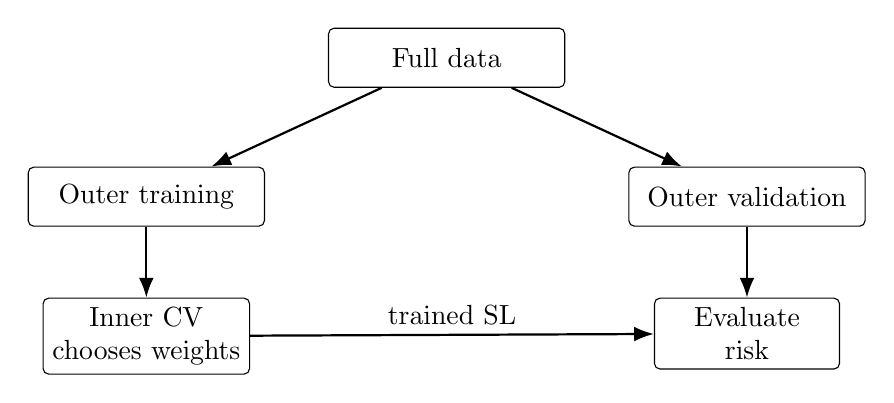
\begin{tikzpicture}[
  node distance=1.1cm,
  box/.style={draw, rounded corners=2pt, minimum width=3.0cm, minimum height=.75cm},
  small/.style={draw, rounded corners=2pt, minimum width=2.35cm, minimum height=.62cm},
  arr/.style={-{Latex[length=2.5mm]}, thick}
]
\node[box] (data) {Full data};
\node[box, below left=1cm and .8cm of data] (outertrain) {Outer training};
\node[box, below right=1cm and .8cm of data] (outervalid) {Outer validation};
\node[small, below=.9cm of outertrain] (inner) {Inner CV\\chooses weights};
\node[small, below=.9cm of outervalid] (risk) {Evaluate\\risk};
\draw[arr] (data) -- (outertrain);
\draw[arr] (data) -- (outervalid);
\draw[arr] (outertrain) -- (inner);
\draw[arr] (inner) -- node[above] {trained SL} (risk);
\draw[arr] (outervalid) -- (risk);
\end{tikzpicture}
\caption{Nested cross-validation evaluates the entire Super Learner procedure.}
\label{fig:ch6-nested-cv}
\end{figure}

If the same folds used to choose weights were also used to evaluate the final Super
Learner, the risk estimate would be optimistic. Nested cross-validation avoids this by
holding out outer validation observations from every part of fitting and weight
selection.

\subsection{Cross-Validated Risk Estimates}

\texttt{CV.SuperLearner()} returns risk estimates for:
\begin{itemize}
\item each candidate algorithm;
\item the discrete Super Learner;
\item the ensemble Super Learner.
\end{itemize}

For continuous outcomes with squared-error loss, the risk is estimated mean squared
prediction error:
\[
\widehat R_{CV}
=
\frac{1}{n}\sum_{i=1}^n
\{Y_i-\hat Q_{-v(i)}(A_i,W_i)\}^2,
\]
where $\hat Q_{-v(i)}$ denotes the prediction rule trained without the outer validation
fold containing observation $i$.

\subsection{Confidence Intervals for Risk}

Plots from \texttt{CV.SuperLearner()} often display estimated risk and approximate
confidence intervals. These intervals quantify uncertainty in the estimated predictive
risk, not uncertainty in a causal effect. They are useful for judging whether apparent
risk differences are meaningful or mostly noise.

If two algorithms have very similar risk estimates with overlapping intervals, it is not
reasonable to claim that one is clearly better. The ensemble can still use both, or put
weight on only one, depending on the metalearner optimization.

\subsection{Discrete Super Learner}

The discrete Super Learner is the single candidate with the best cross-validated risk.
When evaluating results, it is helpful to compare:
\[
\text{best single candidate},\qquad
\text{discrete Super Learner},\qquad
\text{ensemble Super Learner}.
\]
In some datasets, the ensemble improves on all individual candidates. In others, the
best single candidate performs about as well as the ensemble.

\subsection{Comparing Super Learner to Candidate Algorithms}

The following questions guide interpretation:
\begin{itemize}
\item Does the ensemble have lower estimated risk than the best single candidate?
\item Are risk differences large relative to their uncertainty?
\item Which algorithms receive nonzero weight?
\item Are any algorithms unstable, slow, or producing warnings?
\item Does the selected library behave differently for $\Qbar$ than for $g$?
\end{itemize}

\begin{keyidea}
\texttt{SuperLearner()} fits an ensemble for use in analysis. \texttt{CV.SuperLearner()}
evaluates how well the entire ensemble-building procedure predicts new data.
\end{keyidea}

\begin{estimationbox}
For causal effect estimation, nested evaluation is a diagnostic for nuisance-function
prediction. It does not prove that the resulting causal estimator is unbiased, because
causal validity still depends on identification assumptions and adequate positivity.
\end{estimationbox}

\lecture{6.8}{Reporting a Super Learner Analysis}
\label{lec:6-8}

\subsection{Number of Folds}

A report should state the number of cross-validation folds used to train and evaluate
the Super Learner. Common choices are $V=5$ and $V=10$. If nested cross-validation
was used, report both the outer folds and the inner folds.

For example, one might write:
\begin{quote}
The Super Learner was trained using ten-fold cross-validation to choose ensemble
weights. Predictive performance of the full Super Learner procedure was evaluated
using nested ten-fold cross-validation.
\end{quote}

\subsection{Candidate Algorithms}

The candidate library is part of the estimator and must be reported. Include the
algorithm names, important tuning parameters, and whether any variable screening
procedures were paired with each learner.

\[
\begin{array}{lll}
\toprule
\text{Learner} & \text{Description} & \text{Screener}\\
\midrule
\texttt{SL.glm} & \text{main-terms GLM} & \text{All variables}\\
\texttt{SL.mean} & \text{intercept-only model} & \text{All variables}\\
\texttt{SL.ranger} & \text{random forest} & \text{All variables}\\
\texttt{SL.glm} & \text{main-terms GLM} & \texttt{screen.corP}\\
\bottomrule
\end{array}
\]

Large libraries are often best placed in an appendix table.

\subsection{Ensemble Construction}

State whether the analysis used a discrete Super Learner or an ensemble Super
Learner. For ensemble Super Learner, describe the metalearner. For continuous
outcomes, a convex least-squares ensemble is common. For binary outcomes or
propensity scores, a logistic-linear ensemble minimizing negative log-likelihood is
often appropriate.

\subsection{Loss Functions}

The loss function determines what the Super Learner is optimizing. Reports should
state the loss separately for each nuisance function:
\begin{itemize}
\item outcome regression with continuous $Y$: mean squared-error loss;
\item outcome regression with binary $Y$: Bernoulli negative log-likelihood or
another valid binary-outcome loss;
\item propensity score: Bernoulli negative log-likelihood for treatment prediction.
\end{itemize}

\subsection{Cross-Validated Risk Summaries}

Risk summaries should include the Super Learner, the discrete Super Learner, and the
candidate algorithms. A clear table includes the risk estimate, an uncertainty summary
when available, and the ensemble weight.

\[
\begin{array}{lccc}
\toprule
\text{Learner} & \text{CV risk} & \text{Weight} & \text{Comment}\\
\midrule
\texttt{SL.glm\_All} & 1.03 & 0.40 & \text{stable benchmark}\\
\texttt{SL.mean\_All} & 2.72 & 0.00 & \text{intercept only}\\
\texttt{SL.quadglm\_All} & 1.05 & 0.60 & \text{quadratic terms}\\
\text{Super Learner} & 1.01 & -- & \text{ensemble}\\
\bottomrule
\end{array}
\]

\subsection{Sensitivity Analyses}

Super Learner results depend on the candidate library, loss function, and
cross-validation design. Sensitivity analyses can examine whether conclusions change
when:
\begin{itemize}
\item additional flexible learners are added;
\item unstable or extremely slow learners are removed;
\item the number of folds is changed;
\item required confounders are forced into every candidate;
\item alternative reasonable losses are used;
\item propensity score learners producing extreme weights are excluded or modified.
\end{itemize}

\subsection{Methods Write-Up}

A concise methods paragraph for an outcome regression might read:

\begin{quote}
The outcome regression was estimated using Super Learner. Candidate algorithms
included generalized linear models, penalized regression, generalized additive models,
random forests, and multivariate adaptive regression splines, with selected learners
paired with pre-specified screening rules. Ensemble weights were chosen to minimize
ten-fold cross-validated mean squared-error loss using a convex least-squares
metalearner.
\end{quote}

For a propensity score:

\begin{quote}
The propensity score was estimated using Super Learner with treatment as the outcome
and baseline covariates as predictors. Ensemble weights were chosen to minimize
ten-fold cross-validated Bernoulli negative log-likelihood using a logistic-linear
metalearner.
\end{quote}

\subsection{Results Write-Up}

A results paragraph should summarize which learners contributed meaningfully and how
the ensemble compared with individual candidates:

\begin{quote}
For the outcome regression, the Super Learner placed nonzero weight on five
candidate algorithms, with the largest weights assigned to a random forest and a
generalized additive model. Nested cross-validation suggested that the ensemble had
lower estimated risk than any single candidate. For the propensity score, the ensemble
performed similarly to the best individual learner, and predicted treatment
probabilities showed no severe near-zero or near-one instability.
\end{quote}

Avoid interpreting weights as evidence that a scientific model is true. They describe
predictive contributions under the chosen loss.

\subsection{Appendix Tables}

Appendix tables should make the analysis reproducible. At minimum, include:
\begin{itemize}
\item wrapper function names;
\item plain-language descriptions of each algorithm;
\item tuning parameters;
\item screening rules;
\item cross-validated risks;
\item Super Learner weights;
\item software versions when important.
\end{itemize}

\begin{assumptionbox}
Reporting Super Learner details does not replace reporting causal identification
assumptions. The final causal analysis should separately state the target causal
parameter, consistency, exchangeability, positivity, the adjustment set, and the
statistical estimator.
\end{assumptionbox}

\begin{estimationbox}
A complete Super Learner report lets another analyst reconstruct the nuisance
estimation procedure: folds, library, screeners, losses, metalearner, risk summaries,
weights, and sensitivity analyses.
\end{estimationbox}


\chapterheading{7}{Efficient, Doubly Robust Estimation of the ATE}
\lecture{7.1}{Limitations of Naive G-Computation and IPTW}
\label{lec:7-1}

\subsection{Dependence on Nuisance Regression Consistency}

The point-treatment ATE is identified, under consistency, conditional exchangeability,
and positivity, by
\[
\ATE=\E\{\Qbar(1,W)-\Qbar(0,W)\},
\qquad
\Qbar(a,w)=\E(Y\given A=a,W=w),
\]
and also by inverse probability weighting:
\[
\E\{\Ya{a}\}
=
\E\left\{\frac{\ind(A=a)}{g_a(W)}Y\right\},
\qquad
g_a(w)=\Prob(A=a\given W=w).
\]
These formulas lead directly to the estimators studied in Chapter 4:
\[
\psi_{n,G}(a)=\frac{1}{n}\sum_{i=1}^n\Qbar_n(a,W_i)
\]
and
\[
\psi_{n,\IPTW}(a)=
\frac{1}{n}\sum_{i=1}^n
\frac{\ind(A_i=a)}{g_{n,a}(W_i)}Y_i.
\]

Each estimator relies on consistent estimation of a nuisance regression. The
g-computation estimator relies on $\Qbar_n$ being close to $\Qbar$. The IPTW
estimator relies on $g_{n,a}$ being close to $g_a$. If the required nuisance function is
estimated poorly, the resulting causal effect estimator can be biased even in large
samples.

\begin{assumptionbox}
All estimators in this chapter require the same causal identification assumptions as
before:
\[
Y=Y(A),\qquad \Ya{a}\ci A\given W,\qquad 0<\Prob(A=a\given W=w)<1.
\]
Doubly robust estimation improves statistical robustness to nuisance-model
misspecification; it does not remove the need for these causal assumptions.
\end{assumptionbox}

\subsection{Outcome Regression Misspecification}

Suppose the analyst fits a main-terms outcome regression
\[
\Qbar_n(a,w)\approx \beta_0+\beta_1a+\beta_2w,
\]
but the true conditional mean contains an interaction:
\[
\Qbar(a,w)=\beta_0+\beta_1a+\beta_2w+\beta_3aw.
\]
Then $\Qbar_n(1,w)-\Qbar_n(0,w)$ may be systematically wrong for some values of
$w$. Since g-computation averages these predicted contrasts over the covariate
distribution, the resulting ATE estimator can converge to the wrong target.

This is not a small-sample problem. With enough data, the fitted main-terms model may
converge very precisely to the best linear approximation within the misspecified
model class. Precision around the wrong function is still bias for the causal
estimand.

\subsection{Propensity Score Misspecification}

IPTW has a parallel vulnerability. If the propensity score model is misspecified, the
weights
\[
\frac{\ind(A_i=a)}{g_{n,a}(W_i)}
\]
do not create the intended pseudo-population. Some covariate strata may remain
overrepresented and others underrepresented after weighting. In extreme cases, an
incorrect propensity model can also create highly variable weights without correcting
confounding.

For example, if the true propensity score is nonlinear,
\[
g_1(w)=\expit(\alpha_0+\alpha_1w+\alpha_2w^2),
\]
but the analyst fits $\expit(\gamma_0+\gamma_1w)$, the fitted probabilities can be
wrong exactly in regions where treatment assignment is most imbalanced.

\subsection{Flexible Regression Complications}

Super Learning and other flexible regression methods help reduce the risk of severe
misspecification. They allow $\Qbar_n$ and $g_n$ to adapt to nonlinearities,
interactions, and high-dimensional predictor structures.

However, flexible regression creates two new issues. First, flexible learners may
converge more slowly than parametric estimators. Second, their sampling distributions
can be difficult to characterize. The final causal estimator is no longer a simple
average of independent terms with fixed nuisance functions; it contains data-adaptive
estimated functions.

\begin{figure}[H]
\centering
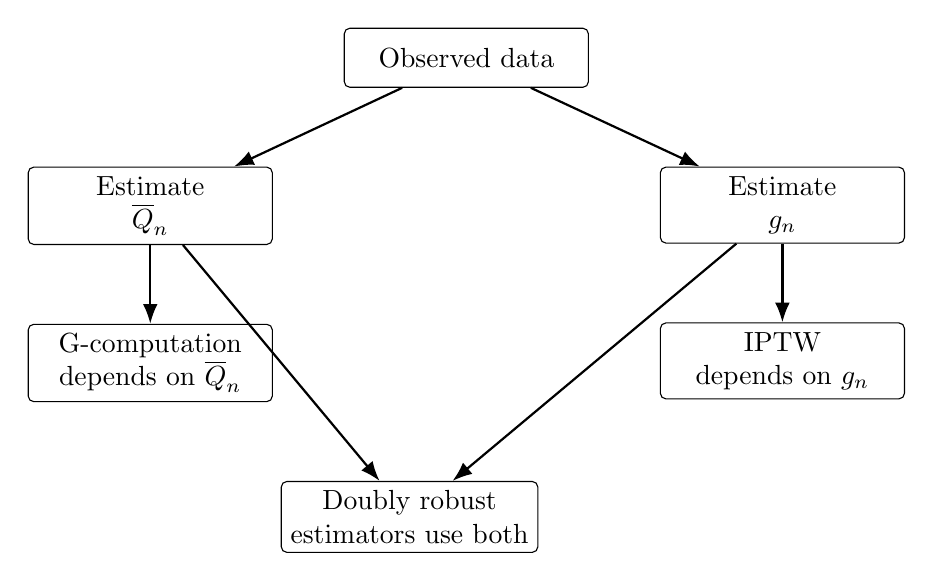
\begin{tikzpicture}[
  node distance=1.15cm,
  box/.style={draw, rounded corners=2pt, minimum width=3.1cm, minimum height=.75cm},
  arr/.style={-{Latex[length=2.5mm]}, thick}
]
\node[box] (data) {Observed data};
\node[box, below left=1cm and .9cm of data] (q) {Estimate\\ $\Qbar_n$};
\node[box, below right=1cm and .9cm of data] (g) {Estimate\\ $g_n$};
\node[box, below=1cm of q] (gc) {G-computation\\ depends on $\Qbar_n$};
\node[box, below=1cm of g] (ipw) {IPTW\\ depends on $g_n$};
\node[box, below right=1cm and .1cm of gc] (aipw) {Doubly robust\\ estimators use both};
\draw[arr] (data) -- (q);
\draw[arr] (data) -- (g);
\draw[arr] (q) -- (gc);
\draw[arr] (g) -- (ipw);
\draw[arr] (q) -- (aipw);
\draw[arr] (g) -- (aipw);
\end{tikzpicture}
\caption{Naive g-computation and IPTW each depend on one nuisance function; doubly robust estimators combine both.}
\label{fig:ch7-nuisance-dependence}
\end{figure}

\subsection{Lack of Standard Inference Basis}

For a simple sample mean, the central limit theorem gives a standard basis for
confidence intervals. For a parametric regression coefficient, classical regression
theory gives approximate standard errors under model assumptions. For naive
g-computation or IPTW with highly adaptive nuisance estimates, neither argument
directly applies without additional work.

The statistical question is not only whether $\psi_n$ is consistent. We also need an
approximation of the form
\[
\sqrt n(\psi_n-\psi)\overset{d}{\longrightarrow}N(0,\sigma^2),
\]
and a consistent estimator of $\sigma^2$. Doubly robust estimators are designed to
have an asymptotic linear representation under appropriate conditions, which gives a
direct route to inference.

\subsection{Bootstrap Limitations}

The nonparametric bootstrap is often useful, but it is not a universal remedy. With
highly adaptive learners, variable selection, non-smooth tuning, or near-positivity
violations, bootstrap distributions can fail to approximate the true sampling
distribution. The bootstrap may also be computationally expensive because every
bootstrap replicate must refit all nuisance functions.

\begin{keyidea}
The limitation of naive g-computation and IPTW is not that they are wrong as
identification formulas. The limitation is that, as estimators, they rely heavily on one
nuisance regression and do not automatically provide stable, valid inference when
that nuisance regression is learned flexibly.
\end{keyidea}

\lecture{7.2}{Augmented IPTW Estimation}
\label{lec:7-2}

\subsection{Combining G-Computation and IPTW}

G-computation and IPTW use different nuisance functions. G-computation predicts
counterfactual outcomes using $\Qbar_n(a,w)$. IPTW reweights observed outcomes
using $g_{n,a}(w)$. Augmented inverse probability weighting combines both ideas in a
single estimator.

The target counterfactual mean is
\[
\psi(a)=\E\{\Ya{a}\}.
\]
Under the usual identification assumptions,
\[
\psi(a)=\E\{\Qbar(a,W)\}
=
\E\left\{\frac{\ind(A=a)}{g_a(W)}Y\right\}.
\]
The AIPTW estimator adds a residual correction to the g-computation estimator, or
equivalently adds an outcome-regression correction to the IPTW estimator.

\subsection{AIPTW Estimator for $\E\{\Yone\}$}

For treatment level $1$, the AIPTW estimator is
\[
\psi_{n,\AIPTW}(1)
=
\frac{1}{n}\sum_{i=1}^n
\left[
\Qbar_n(1,W_i)
+
\frac{\ind(A_i=1)}{g_{n,1}(W_i)}
\{Y_i-\Qbar_n(1,W_i)\}
\right].
\]
The estimated ATE is obtained by forming the analogous estimator for treatment level
$0$ and subtracting:
\[
\widehat{\ATE}_{\AIPTW}
=
\psi_{n,\AIPTW}(1)-\psi_{n,\AIPTW}(0).
\]

\begin{estimationbox}
For binary treatment,
\[
\psi_{n,\AIPTW}(0)
=
\frac{1}{n}\sum_{i=1}^n
\left[
\Qbar_n(0,W_i)
+
\frac{\ind(A_i=0)}{g_{n,0}(W_i)}
\{Y_i-\Qbar_n(0,W_i)\}
\right],
\]
where $g_{n,0}(W_i)=1-g_{n,1}(W_i)$.
\end{estimationbox}

\subsection{IPTW Term}

The estimator can be rearranged as
\[
\psi_{n,\AIPTW}(1)
=
\frac{1}{n}\sum_{i=1}^n
\frac{\ind(A_i=1)}{g_{n,1}(W_i)}Y_i
+
\frac{1}{n}\sum_{i=1}^n
\left\{
1-\frac{\ind(A_i=1)}{g_{n,1}(W_i)}
\right\}
\Qbar_n(1,W_i).
\]
The first term is the usual IPTW estimator of $\E\{\Yone\}$:
\[
\frac{1}{n}\sum_{i=1}^n
\frac{\ind(A_i=1)}{g_{n,1}(W_i)}Y_i.
\]
It uses only observed treated outcomes, weighted by inverse treatment probabilities.

\subsection{Augmentation Term}

The second term,
\[
\frac{1}{n}\sum_{i=1}^n
\left\{
1-\frac{\ind(A_i=1)}{g_{n,1}(W_i)}
\right\}
\Qbar_n(1,W_i),
\]
is the augmentation term. It uses the outcome regression to correct the IPTW
estimator. If the estimated propensity score underweights or overweights certain
treated individuals, the augmentation term offsets part of the resulting distortion.

For example, suppose $Y$ is nonnegative and $g_{n,1}(W)$ tends to underestimate the
true probability of treatment. Then treated individuals receive weights that are too
large, and the IPTW part tends to overshoot. The factor
$1-\ind(A=1)/g_{n,1}(W)$ tends to be negative for treated observations with inflated
weights, so the augmentation term can pull the estimate downward.

\subsection{AIPTW as Augmented G-Computation}

The same estimator can be viewed as g-computation plus a weighted residual average:
\[
\psi_{n,\AIPTW}(1)
=
\underbrace{
\frac{1}{n}\sum_{i=1}^n \Qbar_n(1,W_i)
}_{\text{g-computation}}
+
\underbrace{
\frac{1}{n}\sum_{i=1}^n
\frac{\ind(A_i=1)}{g_{n,1}(W_i)}
\{Y_i-\Qbar_n(1,W_i)\}
}_{\text{augmentation}}.
\]
The augmentation is an average of observed residuals among treated individuals,
weighted to represent the target population. If the outcome regression
$\Qbar_n(1,W)$ systematically overpredicts treated outcomes, then the residuals
$Y-\Qbar_n(1,W)$ tend to be negative, and the augmentation term lowers the
g-computation estimate.

\subsection{Intuition for Bias Correction}

AIPTW uses $\Qbar_n$ to predict missing counterfactual outcomes and uses $g_n$ to
check those predictions against observed residuals in the treatment group that
actually reveals the relevant potential outcome. This creates a bias-correction
mechanism.

\begin{figure}[H]
\centering
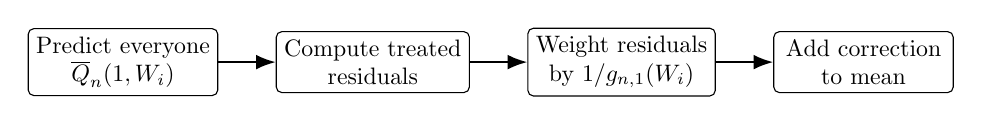
\begin{tikzpicture}[
  scale=.86,
  transform shape,
  node distance=.85cm,
  box/.style={draw, rounded corners=2pt, minimum width=2.65cm, minimum height=.76cm},
  arr/.style={-{Latex[length=2.5mm]}, thick}
]
\node[box] (gcomp) {Predict everyone\\ $\Qbar_n(1,W_i)$};
\node[box, right=of gcomp] (resid) {Compute treated\\ residuals};
\node[box, right=of resid] (weight) {Weight residuals\\ by $1/g_{n,1}(W_i)$};
\node[box, right=of weight] (add) {Add correction\\ to mean};
\draw[arr] (gcomp) -- (resid);
\draw[arr] (resid) -- (weight);
\draw[arr] (weight) -- (add);
\end{tikzpicture}
\caption{AIPTW augments predicted counterfactual means with weighted residual corrections.}
\label{fig:ch7-aiptw-correction}
\end{figure}

\begin{keyidea}
AIPTW is both augmented IPTW and augmented g-computation. The two algebraic forms
are identical, but they highlight different sources of protection: the propensity score
helps correct outcome-regression errors, and the outcome regression helps correct
propensity-score errors.
\end{keyidea}

\lecture{7.3}{Double Robustness}
\label{lec:7-3}

\subsection{Large-Sample Limits of AIPTW}

Double robustness is a large-sample property. Suppose
\[
\Qbar_n(a,w)\overset{p}{\longrightarrow}\Qbar^*(a,w),
\qquad
g_{n,a}(w)\overset{p}{\longrightarrow}g_a^*(w),
\]
where $\Qbar^*$ and $g_a^*$ may or may not equal the true nuisance functions
$\Qbar$ and $g_a$. For treatment level $1$, the AIPTW estimator is expected to
converge to
\[
H(\Qbar^*,g_1^*)
=
\E\left[
\Qbar^*(1,W)
+
\frac{\ind(A=1)}{g_1^*(W)}
\{Y-\Qbar^*(1,W)\}
\right].
\]
The question is when this limit equals the target $\E\{\Yone\}$.

\subsection{Correct Outcome Regression}

First suppose the outcome regression is consistently estimated, so that
\[
\Qbar^*(1,W)=\Qbar(1,W)=\E(Y\given A=1,W).
\]
Then
\[
\begin{aligned}
H(\Qbar,g_1^*)
&=
\E\left[
\Qbar(1,W)
+
\frac{\ind(A=1)}{g_1^*(W)}
\{Y-\Qbar(1,W)\}
\right]\\
&=
\E\left[
\Qbar(1,W)
+
\E\left\{
\frac{\ind(A=1)}{g_1^*(W)}
\{Y-\Qbar(1,W)\}
\given W
\right\}
\right].
\end{aligned}
\]
The inner expectation is zero because
\[
\begin{aligned}
\E\left[
\ind(A=1)\{Y-\Qbar(1,W)\}
\given W
\right]
&=
\Prob(A=1\given W)
\E\{Y-\Qbar(1,W)\given A=1,W\}\\
&=
g_1(W)\{ \Qbar(1,W)-\Qbar(1,W)\}\\
&=0.
\end{aligned}
\]
Therefore,
\[
H(\Qbar,g_1^*)=\E\{\Qbar(1,W)\}=\E\{\Yone\}.
\]
The propensity score limit may be wrong, but the estimator is still consistent if the
outcome regression is correct.

\subsection{Correct Propensity Score}

Now suppose the propensity score is consistently estimated, so
$g_1^*(W)=g_1(W)$, but $\Qbar^*$ may be wrong. Then
\[
\begin{aligned}
H(\Qbar^*,g_1)
&=
\E\left[
\Qbar^*(1,W)
+
\frac{\ind(A=1)}{g_1(W)}
\{Y-\Qbar^*(1,W)\}
\right]\\
&=
\E\left[
\Qbar^*(1,W)
+
\E\left\{
\frac{\ind(A=1)}{g_1(W)}
\{Y-\Qbar^*(1,W)\}
\given W
\right\}
\right].
\end{aligned}
\]
Compute the inner expectation:
\[
\begin{aligned}
\E\left[
\frac{\ind(A=1)}{g_1(W)}
\{Y-\Qbar^*(1,W)\}
\given W
\right]
&=
\frac{1}{g_1(W)}
\E\left[
\ind(A=1)\{Y-\Qbar^*(1,W)\}
\given W
\right]\\
&=
\frac{g_1(W)}{g_1(W)}
\{\Qbar(1,W)-\Qbar^*(1,W)\}\\
&=
\Qbar(1,W)-\Qbar^*(1,W).
\end{aligned}
\]
Substituting back,
\[
H(\Qbar^*,g_1)
=
\E\left[
\Qbar^*(1,W)+\Qbar(1,W)-\Qbar^*(1,W)
\right]
=
\E\{\Qbar(1,W)\}
=
\E\{\Yone\}.
\]

\subsection{Two Chances to Be Consistent}

\begin{definition}[Double robustness]
An estimator is doubly robust for a parameter if it is consistent when either of two
nuisance components is consistently estimated, even if the other nuisance component
is inconsistently estimated.
\end{definition}

For AIPTW, the two nuisance components are $\Qbar$ and $g$. The estimator of
$\E\{\Yone\}$ is consistent if either $\Qbar_n(1,w)$ is consistent for $\Qbar(1,w)$ or
$g_{n,1}(w)$ is consistent for $g_1(w)$. The same reasoning applies to
$\E\{\Yzero\}$ and therefore to the ATE.

\begin{identificationbox}
Under the causal identification assumptions, the AIPTW estimator targets
$\E\{\Ya{a}\}$. Its large-sample limit equals this target if either
$\Qbar_n(a,w)$ consistently estimates $\Qbar(a,w)$ or $g_{n,a}(w)$ consistently
estimates $g_a(w)$.
\end{identificationbox}

\subsection{Concrete Misspecification Example}

A simple data-generating system makes the double-robustness statement
operational. Suppose
\[
  W\sim \operatorname{Uniform}(-2,2),
  \qquad
  A\given W=w\sim \operatorname{Bernoulli}\{g_0(w)\},
\]
where
\[
  g_0(w)=\operatorname{expit}\left\{\frac{3}{2}(w+1)^2-3\right\},
\]
and suppose the conditional mean outcome is
\[
  \Qbar_0(a,w)=\E(Y\given A=a,W=w)=1+a-w-aw.
\]
The true outcome regression contains an interaction between treatment and the
covariate because of the term $-aw$. A main-terms-only outcome regression, such
as $\E(Y\given A,W)=\beta_0+\beta_1A+\beta_2W$, is therefore misspecified. The
true propensity score is nonlinear in $W$ because it contains $(w+1)^2$. A
logistic propensity score model with only a linear term in $W$ is therefore
misspecified.

This example creates four useful cases:
\[
\begin{array}{c|c|c|c}
\text{Outcome model} & \text{Propensity model} & \text{G-computation}
& \text{IPTW}\\
\hline
\text{correct} & \text{correct} & \text{consistent} & \text{consistent}\\
\text{correct} & \text{wrong} & \text{consistent} & \text{biased in general}\\
\text{wrong} & \text{correct} & \text{biased in general} & \text{consistent}\\
\text{wrong} & \text{wrong} & \text{biased in general} & \text{biased in general}
\end{array}
\]
The AIPTW estimator is consistent in the first three rows, but not generally in
the fourth row, where both nuisance models are wrong. In the second row, the augmentation term uses
the correct outcome regression and the residual correction has mean zero. In the
third row, the residual correction is weighted by the correct propensity score
and removes the bias left by the wrong outcome regression. The fourth row is the
warning case: double robustness gives two chances to remove bias, not a
guarantee when both chances fail.

\subsection{Why Double Robustness Is Not a License for Bad Models}

Double robustness is sometimes summarized as ``two chances to get it right.'' That
phrase is useful, but it can be misleading. If both nuisance estimators are poor, the
AIPTW estimator can be badly biased. If both are estimated by simplistic parametric
models that miss important nonlinearities or interactions, there may be no real second
chance.

Double robustness also does not protect against violations of causal assumptions.
Unmeasured confounding, interference, ill-defined interventions, or severe
positivity violations can invalidate the causal interpretation regardless of the
statistical estimator.

\subsection{Connection to Efficiency}

The AIPTW estimator is closely related to the efficient influence function for the
counterfactual mean. When both nuisance functions are consistently estimated at
sufficient rates, AIPTW can achieve the nonparametric efficiency bound for the target
parameter. This means that, in large samples and under regularity conditions, no
regular asymptotically linear estimator can have smaller asymptotic variance in the
nonparametric model.

\begin{keyidea}
Double robustness concerns consistency under one correct nuisance function.
Efficiency concerns variance when both nuisance functions are sufficiently well
estimated. The same augmentation structure is responsible for both properties.
\end{keyidea}

\lecture{7.4}{AIPTW Implementation in R}
\label{lec:7-4}

\subsection{Fitting the Outcome Regression}

To compute AIPTW, first estimate the outcome regression
\[
\Qbar(a,w)=\E(Y\given A=a,W=w).
\]
For a binary outcome, logistic regression is a simple starting point:

\begin{implementationbox}
\begin{lstlisting}[language=R]
# dat contains Y, A, and W variables
or_fit <- glm(Y ~ A + W, data = dat, family = binomial())

dat1 <- dat
dat1$A <- 1
Qbar_1W <- predict(or_fit, newdata = dat1, type = "response")

dat0 <- dat
dat0$A <- 0
Qbar_0W <- predict(or_fit, newdata = dat0, type = "response")
\end{lstlisting}
\end{implementationbox}

The objects \texttt{Qbar\_1W} and \texttt{Qbar\_0W} are estimates of
$\Qbar(1,W_i)$ and $\Qbar(0,W_i)$ for every observed individual.

\subsection{Fitting the Propensity Score}

Next estimate the propensity score:
\[
g_1(w)=\Prob(A=1\given W=w).
\]

\begin{implementationbox}
\begin{lstlisting}[language=R]
ps_fit <- glm(A ~ W, data = dat, family = binomial())

g_1W <- predict(ps_fit, newdata = dat, type = "response")
g_0W <- 1 - g_1W
\end{lstlisting}
\end{implementationbox}

In practice, both $\Qbar_n$ and $g_n$ can be estimated using Super Learner. The
subsequent AIPTW calculations are the same once predicted values are available.

\subsection{Computing AIPTW for $\E\{\Yone\}$}

For treatment level $1$,
\[
\psi_{n,\AIPTW}(1)
=
\frac{1}{n}\sum_{i=1}^n
\left[
\Qbar_n(1,W_i)
+
\frac{\ind(A_i=1)}{g_{n,1}(W_i)}
\{Y_i-\Qbar_n(1,W_i)\}
\right].
\]
In R:

\begin{implementationbox}
\begin{lstlisting}[language=R]
A <- dat$A
Y <- dat$Y

aiptw_ey1 <- mean(Qbar_1W + (A == 1) / g_1W * (Y - Qbar_1W))
\end{lstlisting}
\end{implementationbox}

This expression is often safer than writing separate means for the g-computation and
augmentation terms because it keeps the individual contribution visible.

\subsection{Computing AIPTW for $\E\{\Yzero\}$}

For treatment level $0$,
\[
\psi_{n,\AIPTW}(0)
=
\frac{1}{n}\sum_{i=1}^n
\left[
\Qbar_n(0,W_i)
+
\frac{\ind(A_i=0)}{g_{n,0}(W_i)}
\{Y_i-\Qbar_n(0,W_i)\}
\right].
\]
In R:

\begin{implementationbox}
\begin{lstlisting}[language=R]
aiptw_ey0 <- mean(Qbar_0W + (A == 0) / g_0W * (Y - Qbar_0W))
\end{lstlisting}
\end{implementationbox}

\subsection{Computing the ATE}

The AIPTW ATE estimator is
\[
\widehat{\ATE}_{\AIPTW}
=
\psi_{n,\AIPTW}(1)-\psi_{n,\AIPTW}(0).
\]

\begin{implementationbox}
\begin{lstlisting}[language=R]
aiptw_ate <- aiptw_ey1 - aiptw_ey0
\end{lstlisting}
\end{implementationbox}

Equivalently, define individual ATE contributions
\[
D_{i,n}
=
\Qbar_n(1,W_i)-\Qbar_n(0,W_i)
+
\frac{A_i}{g_{n,1}(W_i)}\{Y_i-\Qbar_n(1,W_i)\}
-
\frac{1-A_i}{g_{n,0}(W_i)}\{Y_i-\Qbar_n(0,W_i)\}.
\]
Then
\[
\widehat{\ATE}_{\AIPTW}=\frac{1}{n}\sum_{i=1}^nD_{i,n}.
\]

\subsection{Practical Coding Workflow}

\begin{estimationbox}
AIPTW coding workflow:
\begin{enumerate}
\item Fit or otherwise estimate $\Qbar_n(A,W)$.
\item Predict $\Qbar_n(1,W_i)$ and $\Qbar_n(0,W_i)$ for every individual.
\item Fit or otherwise estimate $g_{n,1}(W)$.
\item Compute $g_{n,0}(W_i)=1-g_{n,1}(W_i)$.
\item Form $\psi_{n,\AIPTW}(1)$ and $\psi_{n,\AIPTW}(0)$.
\item Subtract to estimate the ATE.
\item Compute influence-function-based standard errors as described in the next
lecture.
\end{enumerate}
\end{estimationbox}

Always check the range of estimated propensity scores. Extremely small values of
$g_{n,1}(W_i)$ among treated observations or $g_{n,0}(W_i)$ among untreated
observations can create unstable residual corrections.

\begin{implementationbox}
\begin{lstlisting}[language=R]
summary(g_1W)
summary(g_0W)
summary((A == 1) / g_1W)
summary((A == 0) / g_0W)
\end{lstlisting}
\end{implementationbox}

\lecture{7.5}{Influence-Function-Based Inference}
\label{lec:7-5}

\subsection{Asymptotic Linearity}

An estimator $\psi_n$ is asymptotically linear for a parameter $\psi$ if it can be
written as
\[
\psi_n-\psi
=
\frac{1}{n}\sum_{i=1}^n D(O_i)+o_p(n^{-1/2}),
\]
where $D(O)$ has mean zero and finite variance. The function $D$ is an influence
function. This representation implies
\[
\sqrt n(\psi_n-\psi)\overset{d}{\longrightarrow}
N\{0,\Var(D(O))\}.
\]

For the counterfactual mean $\psi(1)=\E\{\Yone\}$, the efficient influence function
under the nonparametric point-treatment model is
\[
D_1(O)
=
\frac{\ind(A=1)}{g_1(W)}
\{Y-\Qbar(1,W)\}
+
\Qbar(1,W)-\psi(1).
\]
For $\psi(0)$,
\[
D_0(O)
=
\frac{\ind(A=0)}{g_0(W)}
\{Y-\Qbar(0,W)\}
+
\Qbar(0,W)-\psi(0).
\]
For the ATE, the influence function is
\[
D_{\ATE}(O)=D_1(O)-D_0(O).
\]

\subsection{Estimated Influence Function}

In practice, replace unknown quantities by estimates. For $\psi(1)$:
\[
D_{1,n}(O_i)
=
\frac{\ind(A_i=1)}{g_{n,1}(W_i)}
\{Y_i-\Qbar_n(1,W_i)\}
+
\Qbar_n(1,W_i)-\psi_{n,\AIPTW}(1).
\]
For $\psi(0)$:
\[
D_{0,n}(O_i)
=
\frac{\ind(A_i=0)}{g_{n,0}(W_i)}
\{Y_i-\Qbar_n(0,W_i)\}
+
\Qbar_n(0,W_i)-\psi_{n,\AIPTW}(0).
\]
For the ATE:
\[
D_{\ATE,n}(O_i)=D_{1,n}(O_i)-D_{0,n}(O_i).
\]

\subsection{Variance Estimation}

Estimate the asymptotic variance of $\psi_n(1)$ by the empirical variance of the
estimated influence function:
\[
\hat\tau_1^2
=
\frac{1}{n}\sum_{i=1}^n D_{1,n}(O_i)^2.
\]
The standard error is
\[
\widehat{\mathrm{SE}}\{\psi_n(1)\}
=
\sqrt{\hat\tau_1^2/n}.
\]
For the ATE, use
\[
\hat\tau_{\ATE}^2
=
\frac{1}{n}\sum_{i=1}^n
\left\{
D_{\ATE,n}(O_i)-\bar D_{\ATE,n}
\right\}^2,
\]
where $\bar D_{\ATE,n}=n^{-1}\sum_iD_{\ATE,n}(O_i)$, and
\[
\widehat{\mathrm{SE}}(\widehat{\ATE})
=
\sqrt{\hat\tau_{\ATE}^2/n}.
\]
For AIPTW, $\bar D_{\ATE,n}$ is usually very close to zero by construction, but
centering is harmless and often used in software.

\subsection{Wald Confidence Intervals}

An approximate 95\% Wald interval for $\psi(1)$ is
\[
\psi_{n,\AIPTW}(1)
\pm
1.96\sqrt{\hat\tau_1^2/n}.
\]
An approximate 95\% interval for the ATE is
\[
\widehat{\ATE}_{\AIPTW}
\pm
1.96\,\widehat{\mathrm{SE}}(\widehat{\ATE}).
\]

\begin{implementationbox}
Influence-function standard error for the ATE:
\begin{lstlisting}[language=R]
D1 <- (A == 1) / g_1W * (Y - Qbar_1W) + Qbar_1W - aiptw_ey1
D0 <- (A == 0) / g_0W * (Y - Qbar_0W) + Qbar_0W - aiptw_ey0
Date <- D1 - D0

se_ate <- sqrt(var(Date) / length(Y))
ci_ate <- aiptw_ate + c(-1.96, 1.96) * se_ate
\end{lstlisting}
\end{implementationbox}

\subsection{Hypothesis Tests}

For testing
\[
H_0:\ATE=0
\qquad\text{versus}\qquad
H_1:\ATE\neq 0,
\]
use
\[
Z=\frac{\widehat{\ATE}_{\AIPTW}}
{\widehat{\mathrm{SE}}(\widehat{\ATE})}.
\]
The two-sided Wald p-value is
\[
p=2\{1-\Phi(|Z|)\},
\]
where $\Phi$ is the standard normal distribution function.

\subsection{Coverage in Finite Samples}

Influence-function inference is asymptotic. In finite samples, coverage can be below
or above the nominal level if nuisance regressions are unstable, positivity is weak, or
the sample size is too small for the normal approximation. Coverage often improves as
$n$ grows, provided the nuisance estimators and regularity conditions are adequate.

The estimated influence-function values should be inspected. A few extremely large
values can indicate that confidence intervals are being driven by near-zero propensity
scores or extreme residuals.

\subsection{Simulation Interpretation}

Simulation studies often compare the empirical coverage probability of nominal 95\%
confidence intervals. If 1000 simulated datasets are generated and the 95\% interval
contains the true parameter in 946 of them, the estimated coverage probability is
94.6\%. Such studies reveal finite-sample behavior of the estimator and interval, not
whether a single real-data analysis satisfies the causal assumptions.

\begin{keyidea}
The influence function turns a complicated doubly robust estimator into an approximate
sample mean of mean-zero terms. This is the basis for standard errors, Wald intervals,
and p-values.
\end{keyidea}

\lecture{7.6}{Use in Randomized Trials}
\label{lec:7-6}

\subsection{Why Covariate Adjustment Can Improve Precision}

In a randomized trial, treatment assignment is controlled by design. If treatment is
randomized with probability $p$, then
\[
A\ci W,\qquad \Prob(A=1\given W)=p.
\]
Because treatment is randomized, the unadjusted difference in means is consistent for
the ATE:
\[
\hat\psi_{\mathrm{unadj}}
=
\frac{\sum_iY_i\ind(A_i=1)}{\sum_i\ind(A_i=1)}
-
\frac{\sum_iY_i\ind(A_i=0)}{\sum_i\ind(A_i=0)}.
\]

Covariate adjustment is not required to remove confounding in a well-conducted
randomized trial. It can still improve precision. If baseline covariates strongly
predict the outcome, adjusting for them can remove outcome variation unrelated to
treatment, leading to smaller standard errors.

\subsection{Known Propensity Score Under Randomization}

In a trial with known randomization probability $p$,
\[
g_1(W)=p,\qquad g_0(W)=1-p.
\]
For equal randomization, $p=0.5$. In AIPTW, the known propensity score can be used
instead of estimating $g$:
\[
\psi_{n,\AIPTW}(1)
=
\frac{1}{n}\sum_{i=1}^n
\left[
\Qbar_n(1,W_i)
+
\frac{A_i}{p}\{Y_i-\Qbar_n(1,W_i)\}
\right].
\]
The corresponding expression for $a=0$ uses $(1-A_i)/(1-p)$.

\begin{assumptionbox}
In a randomized trial, exchangeability follows from the randomization design only for
the trial population and intervention actually randomized. Other issues, such as
nonadherence, loss to follow-up, interference, or changes in the target population,
require additional causal assumptions.
\end{assumptionbox}

\subsection{Efficiency Gains}

If $\Qbar_n$ predicts $Y$ well, the residuals $Y-\Qbar_n(A,W)$ are less variable than
the raw outcomes. AIPTW and TMLE use this predictive information while preserving
validness through the known randomization probability. The gain is largest when
baseline covariates are strongly prognostic.

For equal randomization and a well-estimated outcome regression, the precision gain
depends on how much variation in the outcome is explained by baseline covariates and
how treatment effects vary with covariates.

\begin{figure}[H]
\centering
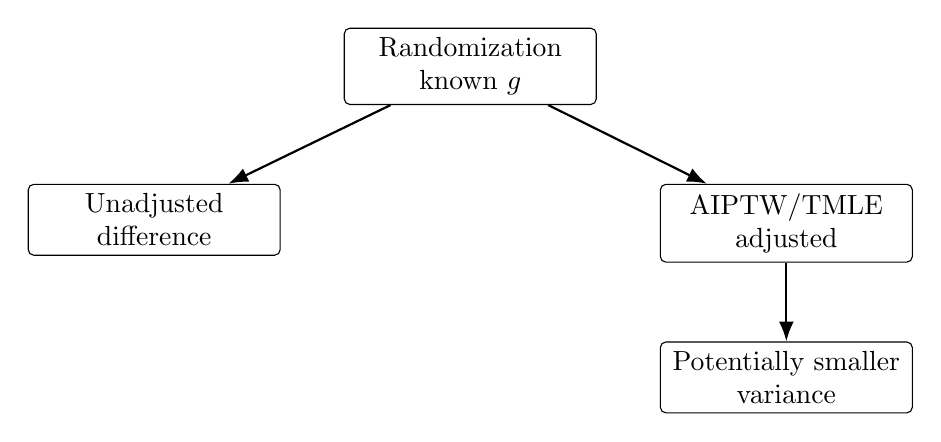
\begin{tikzpicture}[
  node distance=1.35cm,
  box/.style={draw, rounded corners=2pt, minimum width=3.2cm, minimum height=.78cm},
  arr/.style={-{Latex[length=2.5mm]}, thick}
]
\node[box] (rand) {Randomization\\ known $g$};
\node[box, below left=1cm and .8cm of rand] (unadj) {Unadjusted\\ difference};
\node[box, below right=1cm and .8cm of rand] (adj) {AIPTW/TMLE\\ adjusted};
\node[box, below=1cm of adj] (prec) {Potentially smaller\\ variance};
\draw[arr] (rand) -- (unadj);
\draw[arr] (rand) -- (adj);
\draw[arr] (adj) -- (prec);
\end{tikzpicture}
\caption{In randomized trials, adjustment is used for precision rather than confounding control.}
\label{fig:ch7-trial-adjustment}
\end{figure}

\subsection{Outcome Regression in Randomized Trials}

The outcome regression in a trial can include baseline covariates and treatment:
\[
\Qbar(a,w)=\E(Y\given A=a,W=w).
\]
It may include treatment-covariate interactions if effect heterogeneity is plausible.
Because the propensity score is known, double robustness implies that consistency of
AIPTW does not require the outcome regression to be correct. However, a poor outcome
regression can fail to improve precision and may slightly harm finite-sample
performance.

\subsection{When Doubly Robust Methods Are Useful Even Without Confounding}

Doubly robust methods are useful in randomized trials because they provide:
\begin{itemize}
\item design-protected consistency through the known $g$;
\item valid influence-function inference under mild conditions;
\item possible efficiency gains from prognostic baseline covariates;
\item a unified analysis strategy that extends naturally to trials with unequal
randomization or covariate-adaptive designs.
\end{itemize}

\begin{keyidea}
In observational studies, adjustment is needed for identification. In randomized
trials, adjustment is often used for efficiency. The same AIPTW and TMLE formulas
apply, but the known randomization probability gives a particularly strong foundation.
\end{keyidea}

\lecture{7.7}{Targeted Minimum Loss-Based Estimation}
\label{lec:7-7}

\subsection{Compatible Plug-In Estimators}

A compatible plug-in estimator is an estimator that can be written as a parameter
mapping applied to an estimated distribution. For example, the g-computation
estimator
\[
\psi_{n,G}(1)=\frac{1}{n}\sum_{i=1}^n\Qbar_n(1,W_i)
\]
is a plug-in estimator: it applies the counterfactual mean mapping to an estimated
outcome regression and empirical covariate distribution.

IPTW and AIPTW are not generally plug-in estimators in this sense. They can produce
values outside natural parameter bounds. For example, for a binary outcome, a
counterfactual mean should lie in $[0,1]$, but a weighted residual estimator can in
finite samples fall outside that interval.

\subsection{Motivation for TMLE}

Targeted minimum loss-based estimation constructs a plug-in estimator with
influence-function-based bias correction. The idea is to start with an initial outcome
regression $\Qbar_n$, then update it in a targeted way so that the empirical mean of
the efficient influence function is approximately zero.

For $\psi(1)$, the relevant residual equation is
\[
0=
\frac{1}{n}\sum_{i=1}^n
\frac{\ind(A_i=1)}{g_{n,1}(W_i)}
\{Y_i-\Qbar_n^*(1,W_i)\}.
\]
If the updated regression $\Qbar_n^*$ satisfies this equation and remains a valid
conditional mean, then the plug-in estimator
\[
\psi_{n,\TMLE}(1)=\frac{1}{n}\sum_{i=1}^n\Qbar_n^*(1,W_i)
\]
inherits the same first-order bias correction as AIPTW while preserving parameter
constraints.

\subsection{Initial Outcome Regression}

TMLE begins by estimating $\Qbar(A,W)$ and $g_1(W)$. These can be estimated using
parametric models or flexible learners such as Super Learner. For a bounded or binary
outcome, the initial outcome regression should produce predictions inside $(0,1)$.

\subsection{Targeting Step}

For simplicity, consider a binary outcome and estimation of $\psi(1)$. Let
\[
K_i=\logit\{\Qbar_n(1,W_i)\}
\]
be the offset and define the clever covariate
\[
H_1(A_i,W_i)=\frac{\ind(A_i=1)}{g_{n,1}(W_i)}.
\]
Fit a logistic regression with outcome $Y$, offset $K_i$, and single covariate
$H_1(A_i,W_i)$, often using only observations with $A_i=1$ for this one-treatment
update. The fitted coefficient is denoted $\hat\epsilon$. Logistic fluctuation is
directly natural for binary outcomes or outcomes scaled to $[0,1]$; for
continuous unbounded outcomes, TMLE should use an appropriate loss and submodel
or transform the outcome before using a bounded-loss formulation.

\subsection{Clever Covariate}

The clever covariate is called ``clever'' because it is chosen from the efficient
influence function. For treatment level $1$,
\[
H_1(A,W)=\frac{\ind(A=1)}{g_1(W)}.
\]
It weights the outcome-regression fluctuation so that the updated regression solves
the empirical residual equation associated with $\psi(1)$.

\subsection{Updated Regression}

The updated regression for treatment level $1$ is
\[
\Qbar_n^*(1,w)
=
\expit\left[
\logit\{\Qbar_n(1,w)\}
+
\hat\epsilon\frac{1}{g_{n,1}(w)}
\right].
\]
More generally, to target both $\psi(1)$ and $\psi(0)$ simultaneously, define
\[
H_1(A,W)=\frac{A}{g_{n,1}(W)},\qquad
H_0(A,W)=\frac{1-A}{g_{n,0}(W)}.
\]
Fit a logistic fluctuation model with offset $\logit\{\Qbar_n(A,W)\}$ and covariates
$H_1$ and $H_0$. If the fitted coefficients are $\hat\epsilon_1$ and
$\hat\epsilon_0$, then
\[
\Qbar_n^*(a,w)
=
\expit\left[
\logit\{\Qbar_n(a,w)\}
+
\hat\epsilon_1\frac{a}{g_{n,1}(w)}
+
\hat\epsilon_0\frac{1-a}{g_{n,0}(w)}
\right].
\]

\subsection{TMLE Estimate}

The TMLE counterfactual means are plug-in estimates:
\[
\psi_{n,\TMLE}(1)
=
\frac{1}{n}\sum_{i=1}^n\Qbar_n^*(1,W_i),
\]
\[
\psi_{n,\TMLE}(0)
=
\frac{1}{n}\sum_{i=1}^n\Qbar_n^*(0,W_i),
\]
and
\[
\widehat{\ATE}_{\TMLE}
=
\psi_{n,\TMLE}(1)-\psi_{n,\TMLE}(0).
\]

\begin{implementationbox}
Conceptual TMLE code for a binary outcome:
\begin{lstlisting}[language=R]
H1 <- A / g_1W
H0 <- (1 - A) / g_0W
K  <- qlogis(Qbar_AW)

target_fit <- glm(Y ~ -1 + offset(K) + H1 + H0,
                  family = binomial(),
                  start = c(0, 0))

eps1 <- coef(target_fit)["H1"]
eps0 <- coef(target_fit)["H0"]

Qstar_1W <- plogis(qlogis(Qbar_1W) + eps1 / g_1W)
Qstar_0W <- plogis(qlogis(Qbar_0W) + eps0 / g_0W)

tmle_ate <- mean(Qstar_1W - Qstar_0W)
\end{lstlisting}
\end{implementationbox}

\subsection{TMLE vs AIPTW}

AIPTW and TMLE have the same efficient influence function under standard conditions.
Both are doubly robust for consistency. The key difference is that TMLE is a targeted
plug-in estimator. For bounded outcomes, it respects the natural bounds of the
parameter. It can also have better finite-sample behavior in settings with practical
positivity concerns.

\begin{keyidea}
TMLE updates the initial outcome regression just enough to solve the efficient
influence-function estimating equation, then estimates the causal parameter by
plugging in the updated regression.
\end{keyidea}

\lecture{7.8}{Doubly Robust Inference with Flexible Learners}
\label{lec:7-8}

\subsection{Flexible Nuisance Estimation}

Flexible learners are attractive because they reduce reliance on simple parametric
models for $\Qbar$ and $g$. However, flexible nuisance estimation complicates
inference. Consistency of AIPTW or TMLE can hold if either nuisance function is
consistently estimated, but standard Wald inference usually requires more: a tractable
asymptotic linear expansion with consistently estimable variance.

When both nuisance functions are consistently estimated at adequate rates, standard
AIPTW and standard TMLE often have valid influence-function-based inference. The
harder question is what happens when only one nuisance function is consistently
estimated and flexible methods are used.

\subsection{Standard TMLE}

Standard TMLE targets the efficient influence function equation
\[
\frac{1}{n}\sum_{i=1}^nD_n^*(O_i)\approx 0,
\]
where $D_n^*$ is the efficient influence function with $\Qbar_n^*$ and $g_n$ plugged
in. This targeting step gives TMLE the same first-order expansion as AIPTW when the
nuisance estimators behave well.

Standard TMLE is doubly robust for consistency: if either $\Qbar_n$ or $g_n$ is
consistent, the parameter estimate can still be consistent. But this does not
automatically guarantee valid confidence intervals when the other nuisance estimator
is inconsistent and flexible estimation is used.

\subsection{TMLE for Doubly Robust Inference}

Doubly robust inference means more than doubly robust consistency. It means the
estimator has a usable asymptotic normal distribution and variance estimator even
when only one nuisance component is consistently estimated.

Specialized TMLEs can be constructed to target additional equations beyond the usual
efficient influence-function equation. These methods may update both the outcome
regression and the propensity score, often iteratively, to remove additional second-order
terms that would otherwise prevent valid inference.

The technical details are advanced, but the practical message is clear: standard AIPTW
and standard TMLE should not be assumed to deliver valid inference under arbitrary
flexible nuisance estimation if one nuisance function is badly inconsistent.

\subsection{Sample-Size Effects}

Finite-sample performance depends strongly on sample size. In small samples,
flexible learners can overfit, estimated propensity scores can be unstable, and
influence-function approximations can be poor. As sample size grows, flexible
regression can better approximate the nuisance functions, and coverage of
influence-function intervals often improves.

The rate at which coverage improves depends on the complexity of the true nuisance
functions, the learner library, positivity, and the amount of outcome noise.

\subsection{Coverage Probability}

Coverage probability is the repeated-sampling probability that a confidence interval
contains the true parameter. A nominal 95\% interval has good coverage if, across many
repeated samples, it contains the target about 95\% of the time.

Simulation studies comparing naive g-computation, standard TMLE, and TMLE designed
for doubly robust inference often show that coverage can be poor at small sample
sizes, especially when one nuisance regression is misspecified. Methods designed for
doubly robust inference can improve coverage in such settings, but they are more
complex and require careful implementation.

\subsection{Practical Cautions}

\begin{estimationbox}
Practical guidance for flexible doubly robust estimation:
\begin{itemize}
\item Use rich but pre-specified nuisance-function libraries.
\item Inspect estimated propensity scores and clever covariates for extreme values.
\item Use cross-fitting or sample splitting when required by the estimator's theory.
\item Report whether inference relies on both nuisance functions being consistently
estimated or on a method designed for doubly robust inference.
\item Treat small-sample Wald intervals cautiously when weights or influence-function
values are highly variable.
\end{itemize}
\end{estimationbox}

Flexible learners are valuable, but they do not make inference automatic. The more
adaptive the nuisance estimation procedure, the more important it is to use an
estimator and inference procedure whose theoretical conditions match the analysis.

\begin{keyidea}
Doubly robust consistency says that the point estimator can remain consistent if one
nuisance function is correct. Doubly robust inference is stronger: it asks for valid
standard errors and confidence intervals under that same one-correct-nuisance
scenario.
\end{keyidea}

\begin{assumptionbox}
No amount of flexible nuisance estimation can diagnose unmeasured confounding from
the observed data alone. Doubly robust inference concerns statistical robustness after
identification assumptions have been accepted.
\end{assumptionbox}


\chapterheading{8}{Identification and Inference for Time-Varying Interventions}
\lecture{8.1}{Longitudinal Causal Questions}
\label{lec:8-1}

\subsection{Multi-Timepoint Treatments}

Many important interventions are not single decisions. A patient may take a
medication every day, receive chemotherapy at several cycles, return for repeated
injections, or decide whether to continue a behavioral program at each visit. In
such settings the causal question concerns a \emph{sequence} of treatment
decisions, not only one baseline exposure.

Let time be indexed by $k=0,1,\ldots,K$. At time $k$, an individual has a
recorded history, receives or does not receive treatment, and then continues to
the next time point. The final outcome $Y$ is observed after the last treatment
decision.

\begin{figure}[H]
\centering
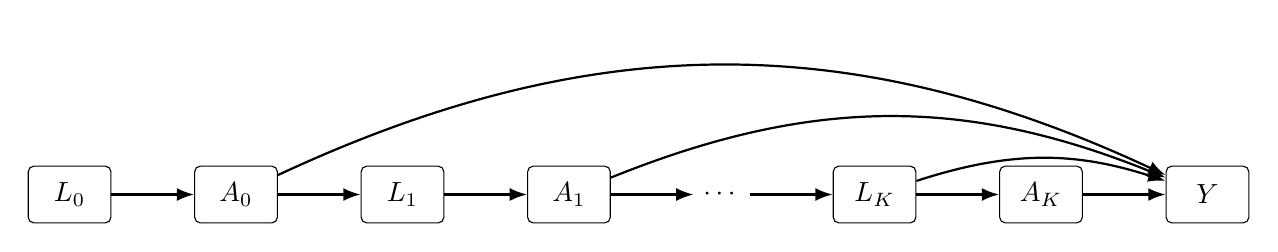
\begin{tikzpicture}[
  node distance=1.05cm,
  box/.style={draw, rounded corners=2pt, minimum width=1.05cm, minimum height=.72cm},
  arr/.style={-{Latex[length=2.2mm]}, thick}
]
\node[box] (L0) {$L_0$};
\node[box, right=of L0] (A0) {$A_0$};
\node[box, right=of A0] (L1) {$L_1$};
\node[box, right=of L1] (A1) {$A_1$};
\node[right=of A1] (dots) {$\cdots$};
\node[box, right=of dots] (LK) {$L_K$};
\node[box, right=of LK] (AK) {$A_K$};
\node[box, right=of AK] (Y) {$Y$};
\draw[arr] (L0) -- (A0);
\draw[arr] (A0) -- (L1);
\draw[arr] (L1) -- (A1);
\draw[arr] (A1) -- (dots);
\draw[arr] (dots) -- (LK);
\draw[arr] (LK) -- (AK);
\draw[arr] (AK) -- (Y);
\draw[arr, bend left=25] (A0) to (Y);
\draw[arr, bend left=22] (A1) to (Y);
\draw[arr, bend left=18] (LK) to (Y);
\end{tikzpicture}
\caption{A generic longitudinal treatment process. Covariates and treatments alternate over time before the final outcome.}
\label{fig:ch8-longitudinal-timeline}
\end{figure}

\begin{keyidea}
A longitudinal causal question asks what would happen if the entire treatment
history were set by an intervention. The unit of intervention is the treatment
regime $\abar=(a_0,\ldots,a_K)$, not a single treatment indicator.
\end{keyidea}

\subsection{Longitudinal Data Structure}

For one individual, write the observed data as
\[
  O=(L_0,A_0,L_1,A_1,\ldots,L_K,A_K,Y).
\]
For $n$ independent individuals, the sample is
\[
  O_1,\ldots,O_n \iid P_0,
\]
where $P_0$ denotes the true observed-data distribution. The variables have the
following roles:
\[
  L_k = \text{covariates recorded at time } k,\qquad
  A_k = \text{treatment at time } k,\qquad
  Y = \text{final outcome}.
\]
The covariate $L_k$ may include new measurements, updated disease severity,
adverse events, adherence information, symptoms, laboratory values, and summaries
of earlier history. It is often vector-valued.

\begin{notation}
We use overbars for histories:
\[
  \Lbar_k=(L_0,\ldots,L_k),\qquad
  \Abar_k=(A_0,\ldots,A_k).
\]
For fixed treatment values,
\[
  \lbar_k=(l_0,\ldots,l_k),\qquad
  \abar_k=(a_0,\ldots,a_k).
\]
When the full treatment history is meant, $\Abar=\Abar_K$ and
$\abar=\abar_K$.
\end{notation}

The timing convention matters. In these notes, $L_k$ is measured before $A_k$.
Thus $A_k$ may depend on $\Lbar_k$ and $\Abar_{k-1}$, but not on future
covariates or future outcomes. This convention is not merely bookkeeping: it
determines what information can be used by a treatment rule at time $k$.

\subsection{$L_k$, $A_k$, and $Y$}

The variable $L_k$ can be both a confounder and an intermediate. For example,
baseline treatment $A_0$ may affect a later biomarker $L_1$, and that biomarker
may affect both later treatment $A_1$ and the outcome $Y$. This feedback is a
central reason why longitudinal causal inference requires special methods.

For two treatment times, the observed data are
\[
  O=(L_0,A_0,L_1,A_1,Y).
\]
A typical causal ordering is
\[
  L_0 \rightarrow A_0 \rightarrow L_1 \rightarrow A_1 \rightarrow Y,
\]
with additional arrows from earlier variables to later variables. The later
covariate $L_1$ is post-treatment with respect to $A_0$, but pre-treatment with
respect to $A_1$.

\subsection{Treatment Regimes}

\begin{definition}[Static treatment regime]
A static treatment regime is a fixed vector
\[
  \abar=(a_0,\ldots,a_K)
\]
that assigns the same treatment value at each time point to every individual,
regardless of the individual's evolving covariate history.
\end{definition}

Examples include ``always treat,'' represented by $(1,1,\ldots,1)$, and
``never treat,'' represented by $(0,0,\ldots,0)$ for a binary treatment.
Other static regimes are possible, such as treating only during the first two
visits and then stopping.

\begin{definition}[Dynamic treatment regime]
A dynamic treatment regime is a sequence of decision rules
\[
  d=(d_0,\ldots,d_K),
\]
where $d_k$ maps the information available at time $k$ to a treatment value:
\[
  A_k=d_k(\Lbar_k,\Abar_{k-1}).
\]
\end{definition}

Dynamic regimes are discussed in detail in \cref{lec:8-11}. For now, the key
point is that longitudinal notation can handle both fixed treatment profiles and
rules that respond to patient history.

\subsection{Counterfactual Outcomes $Y(a_0,\ldots,a_K)$}

\begin{definition}[Longitudinal counterfactual outcome]
For a fixed treatment regime $\abar=(a_0,\ldots,a_K)$, the counterfactual
outcome $Y(\abar)$ is the outcome that would be observed for an individual if,
possibly contrary to fact, treatment were set to $a_k$ at every time
$k=0,\ldots,K$.
\end{definition}

For example, $Y(1,1)$ is the outcome that would be observed under treatment at
both time 0 and time 1. If the observed data contain $A_0=1$ and $A_1=0$, then
$Y(1,1)$ is not directly observed for that individual, even though $Y(1,0)$ may
be linked to the observed outcome by consistency.

Common population-level causal parameters include
\[
  \psi(\abar)=\E\{Y(\abar)\},
\]
and contrasts such as
\[
  \E\{Y(1,\ldots,1)\}-\E\{Y(0,\ldots,0)\}.
\]
For a binary outcome, this contrast is a risk difference comparing two entire
treatment strategies.

\subsection{Clinical Examples}

\begin{example}[Weekly osteoporosis therapy]
Suppose $A_k$ indicates whether a patient took alendronate during week $k$,
where $k=0,\ldots,52$. Let $L_k$ include age, prior fracture status, recent bone
density measurements, thyroid hormone use, side effects, and other clinical
information available at week $k$. Let $Y$ indicate whether hip fracture occurs
within one year. A static contrast of interest is
\[
  \E\{Y(1,1,\ldots,1)\}-\E\{Y(0,0,\ldots,0)\},
\]
the difference in one-year fracture risk under weekly therapy for the whole year
versus no therapy during the year.
\end{example}

\begin{example}[Cancer treatment continuation]
At each chemotherapy cycle, $A_k$ may indicate whether treatment is continued.
The covariate $L_k$ may include tumor response, toxicity, blood counts, and
functional status. Treatment discontinuation may be caused by lack of response,
and lack of response also predicts mortality. Thus later treatment decisions are
confounded by earlier treatment-induced covariates.
\end{example}

\begin{example}[Smoking cessation]
Let $A_k$ indicate whether an individual smokes during month $k$. Respiratory
symptoms recorded in $L_k$ may lead a person to quit smoking and may also be
early signs of disease. A comparison of sustained smoking versus sustained
cessation must handle the fact that symptoms are both affected by prior smoking
and predictive of later smoking and future outcomes.
\end{example}

\lecture{8.2}{Sequential Identification Assumptions}
\label{lec:8-2}

\subsection{Sequential Randomized Trials}

The cleanest way to learn the mean counterfactual outcome $\E\{Y(\abar)\}$ is
to run a trial that randomizes treatment at each time point. In a sequentially
randomized trial, treatment $A_k$ is assigned by a known randomization mechanism
after observing the history available at time $k$.

For a fixed regime $\abar=(a_0,\ldots,a_K)$, randomization implies that treatment
at each time is independent of the relevant counterfactual outcome within the
history strata used by the trial:
\[
  Y(\abar) \ci A_k \given \Lbar_k,\Abar_{k-1}
  \qquad \text{for } k=0,\ldots,K.
\]
At $k=0$, the conditioning set is just $L_0$.

Plainly, among people with the same history up to time $k$, the next treatment
assignment is as if randomized with respect to what would happen under the
regime $\abar$. This is the longitudinal analogue of conditional randomization
for a point treatment.

\subsection{Observational Longitudinal Studies}

In observational longitudinal studies, treatment is not assigned by the analyst.
Patients and clinicians make decisions using information that evolves over time.
Some of this information is measured and included in $\Lbar_k$; some may be
unmeasured.

The inferential challenge is that the observed treatment process may be
informative about future outcomes. For example, a patient may discontinue
chemotherapy because disease is progressing, or a smoker may quit because early
respiratory symptoms have appeared. If those health changes are also associated
with the final outcome, treated and untreated histories are not automatically
comparable.

\subsection{Time-Varying Confounding}

\begin{definition}[Time-varying confounder]
A time-varying confounder is a covariate $L_k$ that predicts later treatment
$A_k$ or $A_{k+1}$ and also predicts the outcome, while possibly being affected
by earlier treatment.
\end{definition}

This dual role is what makes longitudinal confounding different from ordinary
baseline confounding. A later covariate can be necessary for controlling
confounding of later treatment, yet inappropriate to condition on naively when
estimating effects of earlier treatment because it lies on a causal pathway from
earlier treatment to the outcome.

\begin{figure}[H]
\centering
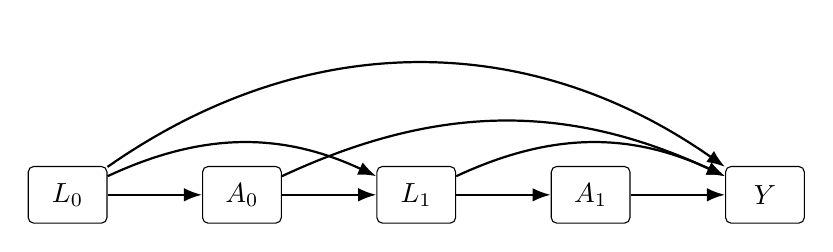
\begin{tikzpicture}[
  node distance=1.2cm,
  box/.style={draw, rounded corners=2pt, minimum width=1.0cm, minimum height=.72cm},
  arr/.style={-{Latex[length=2.3mm]}, thick}
]
\node[box] (L0) {$L_0$};
\node[box, right=of L0] (A0) {$A_0$};
\node[box, right=of A0] (L1) {$L_1$};
\node[box, right=of L1] (A1) {$A_1$};
\node[box, right=of A1] (Y) {$Y$};
\draw[arr] (L0) -- (A0);
\draw[arr] (L0) to[bend left=25] (L1);
\draw[arr] (L0) to[bend left=35] (Y);
\draw[arr] (A0) -- (L1);
\draw[arr] (A0) to[bend left=25] (Y);
\draw[arr] (L1) -- (A1);
\draw[arr] (L1) to[bend left=25] (Y);
\draw[arr] (A1) -- (Y);
\end{tikzpicture}
\caption{Treatment-confounder feedback: $L_1$ is affected by $A_0$ and also confounds the effect of $A_1$ on $Y$.}
\label{fig:ch8-time-varying-confounding}
\end{figure}

\subsection{Sequential Randomization}

\begin{assumptionbox}
For a fixed static regime $\abar=(a_0,\ldots,a_K)$, the sequential
randomization assumption is
\[
  Y(\abar) \ci A_k \given \Lbar_k,\Abar_{k-1}=\abar_{k-1}
  \qquad k=0,\ldots,K.
\]
Equivalently, among individuals whose observed treatment history has followed
the regime through time $k-1$, the next treatment decision is independent of the
counterfactual outcome under the full regime after conditioning on the measured
covariate history.
\end{assumptionbox}

The restriction $\Abar_{k-1}=\abar_{k-1}$ appears because, when identifying
$Y(\abar)$, the relevant risk set at time $k$ consists of individuals who have
remained compatible with the regime up to that time. If a person has already
deviated from the regime, later treatment decisions for that person do not
directly reveal outcomes under the full regime $\abar$ without further modeling.

\subsection{Sequential Exchangeability}

Sequential exchangeability is another name for the same identifying condition.
It emphasizes comparability: after conditioning on the measured history, those
who receive $A_k=a_k$ and those who do not are exchangeable with respect to the
future counterfactual outcome under $\abar$.

For two treatment times and regime $(1,1)$, the assumption is
\[
  Y(1,1) \ci A_0 \given L_0,
\]
and
\[
  Y(1,1) \ci A_1 \given L_0,A_0=1,L_1.
\]
The first line says baseline treatment is unconfounded within baseline covariate
strata. The second says the second treatment is unconfounded within strata of
the history observed among people treated at baseline.

This assumption is not empirically verifiable. The observed data can show
whether treatment depends on measured covariates, but cannot show whether
treatment depends on unmeasured determinants of the counterfactual outcome.

\subsection{Longitudinal Positivity}

\begin{assumptionbox}
For every history with positive probability under the regime of interest,
the probability of receiving the regime-compatible treatment must be positive:
\[
  \Prob(A_k=a_k \given \Lbar_k=\lbar_k,\Abar_{k-1}=\abar_{k-1})>0
  \qquad k=0,\ldots,K.
\]
\end{assumptionbox}

For the always-treated regime $(1,\ldots,1)$ this becomes
\[
  \Prob(A_0=1\given L_0=l_0)>0,
\]
\[
  \Prob(A_1=1\given \Lbar_1=\lbar_1,A_0=1)>0,
\]
and so on through time $K$.

Longitudinal positivity is more fragile than single-timepoint positivity because
probabilities multiply over time. Even if every time-specific probability is
moderate, the probability of observing the entire treatment sequence can be
small:
\[
  \prod_{k=0}^K
  \Prob(A_k=a_k\given \Lbar_k,\Abar_{k-1}=\abar_{k-1}).
\]
Small products lead to unstable inverse probability weights and can make some
static regimes impossible to learn in a given population.

\begin{keyidea}
Identification of a longitudinal regime requires local exchangeability and local
positivity at every treatment decision. A failure at one time point can break
identification of the entire treatment sequence.
\end{keyidea}

\lecture{8.3}{Longitudinal G-Computation Formula}
\label{lec:8-3}

\subsection{Two-Timepoint Derivation}

Consider the observed data
\[
  O=(L_0,A_0,L_1,A_1,Y)
\]
and the target parameter
\[
  \psi(1,1)=\E\{Y(1,1)\}.
\]
Assume the three identifying conditions hold: consistency, sequential
exchangeability, and positivity. The formula repeatedly replaces counterfactual
conditional means with observed conditional means, then averages over the
relevant covariate distributions.

Start with the innermost observed outcome regression:
\[
  \E(Y\given A_1=1,L_1,A_0=1,L_0).
\]
By consistency, among individuals with $A_0=1$ and $A_1=1$, the observed outcome
equals $Y(1,1)$. Therefore
\[
  \E(Y\given A_1=1,L_1,A_0=1,L_0)
  =
  \E\{Y(1,1)\given A_1=1,L_1,A_0=1,L_0\}.
\]
By sequential exchangeability at time 1,
\[
  Y(1,1)\ci A_1\given L_0,A_0=1,L_1,
\]
so
\[
  \E\{Y(1,1)\given A_1=1,L_1,A_0=1,L_0\}
  =
  \E\{Y(1,1)\given L_1,A_0=1,L_0\}.
\]
Define
\[
  \Qbar_2(L_0,L_1)
  =
  \E(Y\given A_1=1,L_1,A_0=1,L_0).
\]
Then
\[
  \Qbar_2(L_0,L_1)
  =
  \E\{Y(1,1)\given L_1,A_0=1,L_0\}.
\]

Now average over the distribution of $L_1$ among those with $A_0=1$ and $L_0$:
\[
  \E\{\Qbar_2(L_0,L_1)\given A_0=1,L_0\}
  =
  \E\{Y(1,1)\given A_0=1,L_0\}.
\]
By sequential exchangeability at time 0,
\[
  Y(1,1)\ci A_0\given L_0,
\]
so
\[
  \E\{Y(1,1)\given A_0=1,L_0\}
  =
  \E\{Y(1,1)\given L_0\}.
\]
Define
\[
  \Qbar_1(L_0)=\E\{\Qbar_2(L_0,L_1)\given A_0=1,L_0\}.
\]
Finally, average over the baseline covariate distribution:
\[
  \E\{\Qbar_1(L_0)\}
  =
  \E\{Y(1,1)\}.
\]

\begin{identificationbox}
For two treatment times,
\[
  \E\{Y(1,1)\}
  =
  \E\left[
    \E\left\{
      \E(Y\given A_1=1,L_1,A_0=1,L_0)
      \given A_0=1,L_0
    \right\}
  \right].
\]
The outer expectation is over the marginal distribution of $L_0$.
\end{identificationbox}

\subsection{Iterated Conditional Expectations}

The formula is a direct application of the tower rule, but the conditioning sets
are chosen according to the intervention. The innermost regression describes the
outcome among individuals who followed the regime through the final treatment.
The next expectation averages over the covariate that would be observed after
following the regime through the previous time. Repeating this process moves
backward through time.

\begin{figure}[H]
\centering
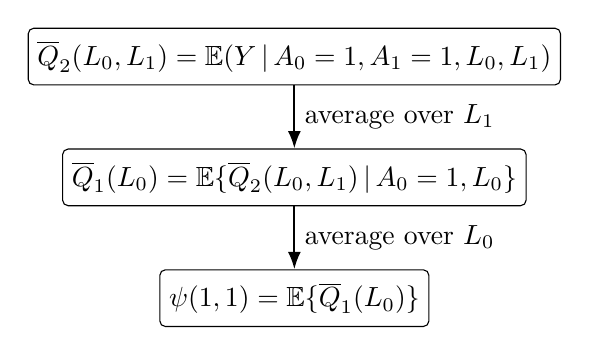
\begin{tikzpicture}[
  node distance=.8cm,
  box/.style={draw, rounded corners=2pt, minimum width=3.2cm, minimum height=.72cm},
  arr/.style={-{Latex[length=2.2mm]}, thick}
]
\node[box] (q2) {$\Qbar_2(L_0,L_1)=\E(Y\given A_0=1,A_1=1,L_0,L_1)$};
\node[box, below=of q2] (q1) {$\Qbar_1(L_0)=\E\{\Qbar_2(L_0,L_1)\given A_0=1,L_0\}$};
\node[box, below=of q1] (q0) {$\psi(1,1)=\E\{\Qbar_1(L_0)\}$};
\draw[arr] (q2) -- node[right] {average over $L_1$} (q1);
\draw[arr] (q1) -- node[right] {average over $L_0$} (q0);
\end{tikzpicture}
\caption{Longitudinal g-computation as backward nested averaging.}
\label{fig:ch8-gcomp-nesting}
\end{figure}

\subsection{General $K$-Timepoint Formula}

For a fixed regime $\abar=(a_0,\ldots,a_K)$, define
\[
  \Qbar_{K+1}(\Lbar_K)
  =
  \E(Y\given \Abar_K=\abar_K,\Lbar_K).
\]
Then recursively define, for $k=K,K-1,\ldots,1$,
\[
  \Qbar_k(\Lbar_{k-1})
  =
  \E\{\Qbar_{k+1}(\Lbar_k)
    \given \Abar_{k-1}=\abar_{k-1},\Lbar_{k-1}\}.
\]
The target mean is
\[
  \psi(\abar)=\E\{\Qbar_1(L_0)\}.
\]

Equivalently, the formula can be displayed as nested expectations:
\[
  \E\{Y(\abar)\}
  =
  \E\left[
  \E\left[
  \cdots
  \E\left[
  \E(Y\given \Abar_K=\abar_K,\Lbar_K)
  \given \Abar_{K-1}=\abar_{K-1},\Lbar_{K-1}
  \right]
  \cdots
  \given A_0=a_0,L_0
  \right]\right].
\]

\subsection{Sequential Outcome Regressions}

The functions $\Qbar_{K+1},\Qbar_K,\ldots,\Qbar_1$ are called sequential outcome
regressions. They are not all regressions of $Y$. Only $\Qbar_{K+1}$ is the
conditional mean of the observed outcome. The earlier regressions use later
predicted values as pseudo-outcomes.

For $K=1$, the sequence is:
\[
  \Qbar_2(L_0,L_1)=\E(Y\given A_0=a_0,A_1=a_1,L_0,L_1),
\]
\[
  \Qbar_1(L_0)=\E\{\Qbar_2(L_0,L_1)\given A_0=a_0,L_0\},
\]
\[
  \psi(a_0,a_1)=\E\{\Qbar_1(L_0)\}.
\]

\subsection{Interpretation of Nested Expectations}

Each expectation performs one of two tasks. First, it replaces the observed
treatment assignment with the regime value. Second, it averages over covariates
that would naturally arise after earlier parts of the regime.

For the regime $(1,1)$, the inner regression asks: among people who received
treatment at both times and had a given covariate history, what was the mean
outcome? The next regression asks: among people who received treatment at time
0 and had a given $L_0$, what covariate histories $L_1$ occurred, and what
outcomes would those histories imply if treatment also occurred at time 1? The
final average transports these predicted means to the baseline target population.

\begin{keyidea}
Longitudinal g-computation is standardization over time. It standardizes the
final outcome regression over the sequence of covariate distributions generated
under the intervention history.
\end{keyidea}

\lecture{8.4}{Longitudinal IPTW Formula}
\label{lec:8-4}

\subsection{Generalized Propensity Scores}

For a point treatment, the propensity score is the conditional probability of
receiving the observed or target treatment. In a longitudinal study, there is a
time-specific treatment mechanism at every decision time.

\begin{definition}[Generalized propensity score]
For a binary treatment and fixed regime $\abar=(a_0,\ldots,a_K)$, define
\[
  g_k(a_k\given \lbar_k,\abar_{k-1})
  =
  \Prob(A_k=a_k\given \Lbar_k=\lbar_k,\Abar_{k-1}=\abar_{k-1}).
\]
For the always-treated regime, write
\[
  g_k(\lbar_k)
  =
  \Prob(A_k=1\given \Lbar_k=\lbar_k,\Abar_{k-1}=\mathbf{1}_k).
\]
\end{definition}

The time-specific propensity score is local: it concerns the treatment decision
at time $k$ among individuals whose previous treatment history is compatible
with the regime.

\subsection{Composite Treatment Probabilities}

The probability of receiving an entire treatment profile is the product of the
time-specific probabilities. For regime $\abar$ define
\[
  \gbar_K(\Lbar_K)
  =
  \prod_{k=0}^K
  g_k(a_k\given \Lbar_k,\Abar_{k-1}=\abar_{k-1}).
\]
For the always-treated regime this is
\[
  \gbar_K(\Lbar_K)
  =
  g_0(L_0)g_1(\Lbar_1)\cdots g_K(\Lbar_K).
\]

This product is the probability that a person with the realized covariate
history would follow the regime through all treatment times, under the observed
treatment mechanism.

\subsection{Treatment-Regime Weights}

The inverse probability weight for a regime $\abar$ is
\[
  H_{\abar}
  =
  \frac{\ind(\Abar_K=\abar_K)}{\gbar_K(\Lbar_K)}.
\]
For the always-treated regime,
\[
  H_{\mathbf{1}}
  =
  \frac{A_0A_1\cdots A_K}
       {g_0(L_0)g_1(\Lbar_1)\cdots g_K(\Lbar_K)}.
\]

The numerator selects individuals whose observed treatment history matches the
regime. The denominator upweights those individuals by the inverse probability
of observing that full history.

\begin{figure}[H]
\centering
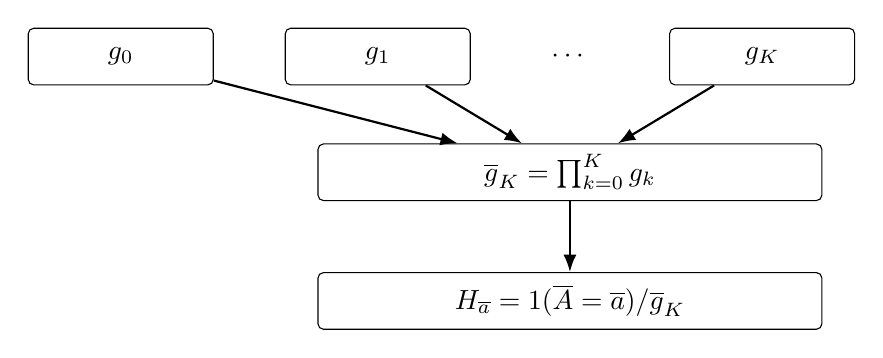
\begin{tikzpicture}[
  node distance=.9cm,
  box/.style={draw, rounded corners=2pt, minimum width=2.35cm, minimum height=.72cm},
  arr/.style={-{Latex[length=2.2mm]}, thick}
]
\node[box] (p0) {$g_0$};
\node[box, right=of p0] (p1) {$g_1$};
\node[right=of p1] (dots) {$\cdots$};
\node[box, right=of dots] (pK) {$g_K$};
\node[box, below=of dots, minimum width=6.4cm] (prod) {$\gbar_K=\prod_{k=0}^K g_k$};
\node[box, below=of prod, minimum width=6.4cm] (w) {$H_{\abar}=\ind(\Abar=\abar)/\gbar_K$};
\draw[arr] (p0) -- (prod);
\draw[arr] (p1) -- (prod);
\draw[arr] (pK) -- (prod);
\draw[arr] (prod) -- (w);
\end{tikzpicture}
\caption{Longitudinal IPTW uses the product of time-specific treatment probabilities.}
\label{fig:ch8-longitudinal-iptw}
\end{figure}

\subsection{IPTW Identification for Treatment Profiles}

\begin{identificationbox}
Under consistency, sequential exchangeability, and longitudinal positivity,
\[
  \E\{Y(\abar)\}
  =
  \E\left[
    \frac{\ind(\Abar_K=\abar_K)}
         {\prod_{k=0}^K g_k(a_k\given \Lbar_k,\Abar_{k-1}=\abar_{k-1})}
    Y
  \right].
\]
For the always-treated regime,
\[
  \E\{Y(1,\ldots,1)\}
  =
  \E\left[
    \frac{A_0A_1\cdots A_K}
         {g_0(L_0)g_1(\Lbar_1)\cdots g_K(\Lbar_K)}
    Y
  \right].
\]
\end{identificationbox}

The formula creates a pseudo-population in which following the regime is no
longer associated with measured history. Individuals with rare regime-compatible
histories receive larger weights because they represent many similar individuals
who did not follow the regime.

\subsection{Positivity Problems Over Time}

Longitudinal weights can become unstable quickly. If $K=5$ and each
time-specific probability equals $0.5$, then the composite probability is
$0.5^6=0.015625$. The corresponding weight is $64$ for an individual who
follows the whole regime. If some probabilities are smaller, weights can be much
larger.

There are two kinds of positivity problems:
\begin{itemize}
  \item \textbf{Structural violations}: a treatment sequence is impossible for
  some history, such as a contraindicated drug after severe toxicity.
  \item \textbf{Practical violations}: the sequence is possible in principle but
  rarely observed in the sample.
\end{itemize}
Both problems are more common as the number of treatment times grows.

\subsection{Equivalence with G-Computation}

The IPTW and g-computation formulas identify the same counterfactual mean. The
equivalence follows by repeated use of iterated expectation.

For the always-treated regime, let
\[
  \Qbar_{K+1}(\Lbar_K)=\E(Y\given \Abar_K=\mathbf{1}_{K+1},\Lbar_K).
\]
Then
\[
\begin{aligned}
&\E\left[
  \frac{A_0\cdots A_K}{g_0(\Lbar_0)\cdots g_K(\Lbar_K)}Y
\right] \\
&=
\E\left[
  \frac{A_0\cdots A_K}{g_0(\Lbar_0)\cdots g_K(\Lbar_K)}
  \E(Y\given \Lbar_K,\Abar_K)
\right] \\
&=
\E\left[
  \frac{A_0\cdots A_K}{g_0(\Lbar_0)\cdots g_K(\Lbar_K)}
  \Qbar_{K+1}(\Lbar_K)
\right].
\end{aligned}
\]
Now condition on $\Lbar_K,\Abar_{K-1}$. Since
\[
  \E(A_K\given \Lbar_K,\Abar_{K-1}=\mathbf{1}_K)=g_K(\Lbar_K),
\]
the factor $A_K/g_K(\Lbar_K)$ averages to one among those compatible with the
past regime. Therefore the last expression becomes
\[
  \E\left[
  \frac{A_0\cdots A_{K-1}}{g_0(\Lbar_0)\cdots g_{K-1}(\Lbar_{K-1})}
  \E\{\Qbar_{K+1}(\Lbar_K)\given \Lbar_{K-1},\Abar_{K-1}=\mathbf{1}_K\}
  \right].
\]
The conditional expectation is $\Qbar_K(\Lbar_{K-1})$. Repeating the same
argument removes $A_{K-1}/g_{K-1}$, then $A_{K-2}/g_{K-2}$, and so on, yielding
\[
  \E\{\Qbar_1(L_0)\},
\]
which is the g-computation formula.

\begin{keyidea}
IPTW and g-computation are two representations of the same identifying
functional. G-computation integrates outcome regressions forward through the
covariate process; IPTW reweights observed regime followers to represent the
target population.
\end{keyidea}

\lecture{8.5}{Failure of Naive Regression}
\label{lec:8-5}

\subsection{Regression Coefficients in Single-Timepoint Settings}

Even in a point-treatment setting, a regression coefficient is not automatically
an average treatment effect. Suppose
\[
  \E(Y\given A=a,W=w)=\beta_0+\beta_1 a+\beta_2 w.
\]
Then
\[
  \E(Y\given A=1,W=w)-\E(Y\given A=0,W=w)=\beta_1
\]
for every $w$, and the standardized mean difference is also $\beta_1$:
\[
  \E\{\E(Y\given A=1,W)-\E(Y\given A=0,W)\}=\beta_1.
\]
This special equality depends on the linear model and the absence of treatment
effect modification by $W$.

\subsection{Linear Models Without Interactions}

When a linear model has no interaction between treatment and covariates, the
treatment coefficient is a constant conditional mean contrast. Under the usual
identification assumptions, it can equal the g-computation estimate of the ATE.
This is a special case, not a general rule.

\subsection{Linear Models With Interactions}

If the conditional mean includes an interaction,
\[
  \E(Y\given A=a,W=w)=\beta_0+\beta_1a+\beta_2w+\beta_3aw,
\]
then the conditional contrast is
\[
  \E(Y\given A=1,W=w)-\E(Y\given A=0,W=w)=\beta_1+\beta_3w.
\]
The marginal standardized contrast is
\[
  \E(\beta_1+\beta_3W)=\beta_1+\beta_3\E(W).
\]
Thus $\beta_1$ is the conditional contrast at $W=0$, not the average treatment
effect unless $\E(W)=0$ or $\beta_3=0$.

\subsection{Logistic Models}

For binary outcomes, logistic regression is nonlinear:
\[
  \E(Y\given A=a,W=w)=\expit(\beta_0+\beta_1a+\beta_2w).
\]
The risk difference at covariate value $w$ is
\[
  \expit(\beta_0+\beta_1+\beta_2w)-\expit(\beta_0+\beta_2w),
\]
and the marginal risk difference is
\[
  \E\left[
    \expit(\beta_0+\beta_1+\beta_2W)-\expit(\beta_0+\beta_2W)
  \right].
\]
The coefficient $\beta_1$ is a conditional log-odds ratio parameter, not a risk
difference and not a marginal ATE.

\subsection{Time-Varying Confounder Feedback}

Longitudinal settings introduce a deeper problem. Consider
\[
  L_0 \rightarrow A_0 \rightarrow L_1 \rightarrow A_1 \rightarrow Y,
\]
where $L_1$ also affects $Y$. A regression of $Y$ on $A_0,L_1,A_1$ conditions
on $L_1$. This may be useful for estimating the effect of $A_1$, because $L_1$
confounds the $A_1$--$Y$ relation. But it blocks part of the effect of $A_0$ on
$Y$ that operates through $L_1$.

\begin{figure}[H]
\centering
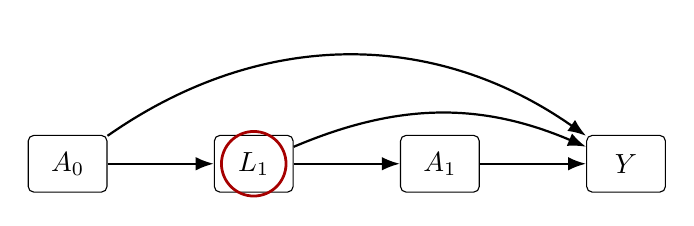
\begin{tikzpicture}[
  node distance=1.35cm,
  box/.style={draw, rounded corners=2pt, minimum width=1.0cm, minimum height=.72cm},
  arr/.style={-{Latex[length=2.3mm]}, thick},
  block/.style={draw=red!65!black, line width=1pt, circle, minimum size=.82cm}
]
\node[box] (A0) {$A_0$};
\node[box, right=of A0] (L1) {$L_1$};
\node[box, right=of L1] (A1) {$A_1$};
\node[box, right=of A1] (Y) {$Y$};
\draw[arr] (A0) -- (L1);
\draw[arr] (L1) -- (A1);
\draw[arr] (A1) -- (Y);
\draw[arr, bend left=23] (L1) to (Y);
\draw[arr, bend left=35] (A0) to (Y);
\node[block] at (L1) {};
\end{tikzpicture}
\caption{Conditioning on $L_1$ can block the mediated path from $A_0$ to $Y$ while controlling confounding for $A_1$.}
\label{fig:ch8-naive-blocking}
\end{figure}

\subsection{A Numerical Data-Generating Example}

Suppose
\[
  A_0\sim \operatorname{Bernoulli}(0.5),
\]
\[
  L_1\given A_0=a_0 \sim N(1+a_0,1),
\]
\[
  A_1\given L_1=l_1,A_0=a_0
  \sim \operatorname{Bernoulli}\{\expit(-1+l_1+a_0)\},
\]
and
\[
  Y\given A_1=a_1,L_1=l_1,A_0=a_0
  \sim N(1+a_1+2l_1,1).
\]
The mean outcome regression does not contain $A_0$ directly. Nevertheless,
$A_0$ has a causal effect because it shifts $L_1$, and $L_1$ affects $Y$.

Using g-computation,
\[
\begin{aligned}
  \E\{Y(1,1)\}
  &=\E\{\E(Y\given A_1=1,L_1,A_0=1)\given A_0=1\}\\
  &=\E(2+2L_1\given A_0=1)=2+2(2)=6,
\end{aligned}
\]
because $\E(L_1\given A_0=1)=2$. Similarly,
\[
  \E\{Y(1,0)\}=5,\qquad
  \E\{Y(0,1)\}=4,\qquad
  \E\{Y(0,0)\}=3.
\]
Therefore the effect of changing $A_0$ from 0 to 1 while holding $A_1=1$ is
\[
  \E\{Y(1,1)-Y(0,1)\}=2.
\]

Now fit the correctly specified conditional mean regression
\[
  \E(Y\given A_1,L_1,A_0)=1+A_1+2L_1+0\cdot A_0.
\]
The coefficient on $A_0$ is zero because the regression conditions on $L_1$.
Reading the $A_0$ coefficient as the causal effect of baseline treatment would
therefore be wrong.

\subsection{Blocking Causal Pathways by Conditioning on Intermediates}

The problem is not that regression is useless. The problem is using one
conditional regression as if it were the causal estimand. Sequential
g-computation uses regressions carefully: it conditions on $L_1$ in the final
outcome regression and then averages over the distribution of $L_1$ that would
arise under each baseline treatment. A naive regression coefficient conditions
on $L_1$ and stops there.

\begin{keyidea}
In longitudinal studies, the same covariate can be a confounder for later
treatment and a mediator for earlier treatment. Ordinary regression adjustment
cannot generally handle this feedback by reading off coefficients.
\end{keyidea}

\lecture{8.6}{IPTW Estimation for Time-Varying Interventions}
\label{lec:8-6}

\subsection{Estimating Time-Specific Propensity Scores}

The longitudinal IPTW identification formula suggests a direct estimator. For a
fixed regime $\abar$, estimate each treatment mechanism
\[
  g_k(a_k\given \Lbar_k,\Abar_{k-1}=\abar_{k-1})
\]
and then average the weighted outcomes among individuals whose observed
treatment history matches the regime.

For two treatment times and binary treatments, estimate
\[
  g_0(a_0\given L_0)=\Prob(A_0=a_0\given L_0),
\]
and
\[
  g_1(a_1\given L_0,A_0=a_0,L_1)
  =
  \Prob(A_1=a_1\given L_0,A_0=a_0,L_1).
\]
The models for these probabilities may be logistic regressions, Super Learner
fits, or other binary regression estimators.

\subsection{Constructing Cumulative Weights}

For subject $i$, define the estimated regime probability
\[
  \gbar_{n,K,i}(\abar)
  =
  \prod_{k=0}^K
  g_{n,k}(a_k\given \Lbar_{k,i},\Abar_{k-1,i}=\abar_{k-1}).
\]
The estimated weight is
\[
  H_{n,i}(\abar)
  =
  \frac{\ind(\Abar_{K,i}=\abar_K)}{\gbar_{n,K,i}(\abar)}.
\]

\begin{estimationbox}
The IPTW estimator of the counterfactual mean under regime $\abar$ is
\[
  \psi_{n,\IPTW}(\abar)
  =
  \frac{1}{n}\sum_{i=1}^n
  H_{n,i}(\abar)Y_i.
\]
An ATE comparing regimes $\abar$ and $\abar'$ is estimated by
\[
  \psi_{n,\IPTW}(\abar)-\psi_{n,\IPTW}(\abar').
\]
\end{estimationbox}

Some analysts use stabilized weights to reduce variance. For a static regime,
a stabilized weight has a numerator that models the probability of the treatment
history using less covariate information, for example
\[
  \prod_{k=0}^K
  \Prob(A_k=a_k\given \Abar_{k-1}=\abar_{k-1}),
\]
divided by the full denominator. Stabilization changes the variance properties,
but the denominator is still the part that removes measured confounding.

\subsection{Estimating Counterfactual Means}

For $K=1$ and regime $(1,1)$,
\[
  \psi_{n,\IPTW}(1,1)
  =
  \frac{1}{n}\sum_{i=1}^n
  \frac{\ind(A_{0i}=1,A_{1i}=1)}
       {g_{n,0}(1\given L_{0i})
        g_{n,1}(1\given L_{0i},A_0=1,L_{1i})}
  Y_i.
\]
For regime $(1,0)$,
\[
  \psi_{n,\IPTW}(1,0)
  =
  \frac{1}{n}\sum_{i=1}^n
  \frac{\ind(A_{0i}=1,A_{1i}=0)}
       {g_{n,0}(1\given L_{0i})
        \{1-g_{n,1}(1\given L_{0i},A_0=1,L_{1i})\}}
  Y_i.
\]
The same pattern applies to $(0,1)$ and $(0,0)$, with the appropriate
probabilities in the denominator.

\subsection{R Implementation}

The following code implements the two-timepoint estimator in a simulated data
set with variables `A0`, `L1`, `A1`, and `Y`. The treatment at time 0 is
randomized in this example, so the first propensity model is intercept-only.

\begin{lstlisting}[language=R]
# time-0 treatment mechanism
ps0 <- glm(A0 ~ 1, family = binomial())
g_0 <- predict(ps0, type = "response")

# time-1 treatment mechanism
ps1 <- glm(A1 ~ L1 + A0, family = binomial())

# P(A1 = 1 | A0 = 1, L1 = L1_i)
g_1_A0_1 <- predict(
  ps1,
  newdata = data.frame(A0 = 1, L1 = L1),
  type = "response"
)

# P(A1 = 1 | A0 = 0, L1 = L1_i)
g_1_A0_0 <- predict(
  ps1,
  newdata = data.frame(A0 = 0, L1 = L1),
  type = "response"
)

EY_11 <- mean((A0 == 1 & A1 == 1) / (g_0 * g_1_A0_1) * Y)
EY_10 <- mean((A0 == 1 & A1 == 0) / (g_0 * (1 - g_1_A0_1)) * Y)
EY_01 <- mean((A0 == 0 & A1 == 1) / ((1 - g_0) * g_1_A0_0) * Y)
EY_00 <- mean((A0 == 0 & A1 == 0) / ((1 - g_0) * (1 - g_1_A0_0)) * Y)

ate_11_vs_00 <- EY_11 - EY_00
\end{lstlisting}

\subsection{Simulated Examples}

In the data-generating example from \cref{lec:8-5}, the true counterfactual means
are
\[
  \E\{Y(1,1)\}=6,\quad
  \E\{Y(1,0)\}=5,\quad
  \E\{Y(0,1)\}=4,\quad
  \E\{Y(0,0)\}=3.
\]
If the propensity score models are correctly specified and the sample is large,
the IPTW estimates should be close to these values. Discrepancies in finite
samples arise from random error, propensity score estimation error, and weight
instability.

\subsection{Diagnosing Extreme Weights}

Because longitudinal weights multiply inverse probabilities, diagnostics are
essential. At a minimum, inspect:
\begin{itemize}
  \item summaries of each time-specific propensity score;
  \item summaries of the cumulative denominator $\gbar_{n,K}$;
  \item summaries of the final weights $H_{n,i}(\abar)$;
  \item the number of individuals who follow each regime;
  \item whether large weights are concentrated in clinically unusual histories.
\end{itemize}

\begin{lstlisting}[language=R]
w_11 <- (A0 == 1 & A1 == 1) / (g_0 * g_1_A0_1)

summary(g_0)
summary(g_1_A0_1)
summary(w_11)
quantile(w_11, probs = c(.5, .9, .95, .99, 1))
mean(A0 == 1 & A1 == 1)
\end{lstlisting}

Large weights do not automatically imply bias, but they indicate that the
estimate depends heavily on a small number of observations. Truncating weights
can reduce variance but changes the estimand or introduces bias, so it should be
reported as a sensitivity analysis rather than hidden as a default.

\begin{keyidea}
Longitudinal IPTW is simple to compute once time-specific propensity scores are
available, but it can be highly variable because a full treatment history may be
rare even when each individual treatment decision is not rare.
\end{keyidea}

\lecture{8.7}{Sequential Regression G-Computation}
\label{lec:8-7}

\subsection{Backward Recursive Regressions}

Sequential regression is an implementation of the longitudinal g-computation
formula that avoids explicitly estimating the full conditional distribution of
each time-varying covariate. Instead, it works backward from the final outcome.

For $K=1$ and regime $(a_0,a_1)$:
\[
  \Qbar_2(L_0,L_1)=\E(Y\given A_0=a_0,A_1=a_1,L_0,L_1),
\]
\[
  \Qbar_1(L_0)=\E\{\Qbar_2(L_0,L_1)\given A_0=a_0,L_0\},
\]
\[
  \psi(a_0,a_1)=\E\{\Qbar_1(L_0)\}.
\]
Sequential regression estimates $\Qbar_2$, predicts it for all individuals, then
uses those predictions as the outcome in a regression for $\Qbar_1$ among
individuals with $A_0=a_0$.

\begin{figure}[H]
\centering
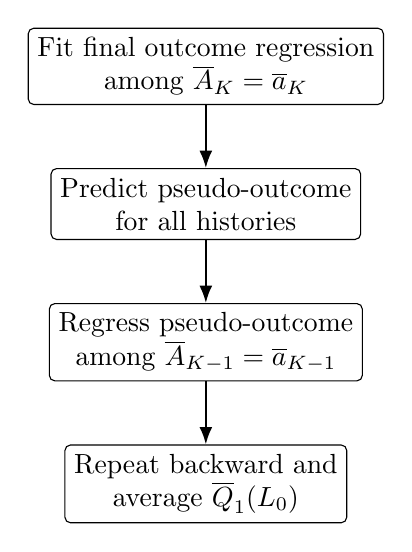
\begin{tikzpicture}[
  node distance=.8cm,
  box/.style={draw, rounded corners=2pt, minimum width=3.5cm, minimum height=.74cm},
  arr/.style={-{Latex[length=2.2mm]}, thick}
]
\node[box] (s1) {Fit final outcome regression\\ among $\Abar_K=\abar_K$};
\node[box, below=of s1] (s2) {Predict pseudo-outcome\\ for all histories};
\node[box, below=of s2] (s3) {Regress pseudo-outcome\\ among $\Abar_{K-1}=\abar_{K-1}$};
\node[box, below=of s3] (s4) {Repeat backward and\\ average $\Qbar_1(L_0)$};
\draw[arr] (s1) -- (s2);
\draw[arr] (s2) -- (s3);
\draw[arr] (s3) -- (s4);
\end{tikzpicture}
\caption{Sequential regression implements g-computation by backward recursion.}
\label{fig:ch8-sequential-regression}
\end{figure}

\subsection{Pseudo-Outcomes}

A pseudo-outcome is a fitted value from a later regression that becomes the
outcome for an earlier regression. In the two-timepoint case:
\begin{enumerate}
  \item Fit a regression for $Y$ among those with $A_0=a_0,A_1=a_1$.
  \item Predict $\Qbar_{2,n}(L_{0i},L_{1i})$ for every individual.
  \item Among those with $A_0=a_0$, regress $\Qbar_{2,n}(L_{0i},L_{1i})$ on
  $L_{0i}$.
  \item Predict $\Qbar_{1,n}(L_{0i})$ for every individual.
  \item Average these predictions.
\end{enumerate}

This is a regression-based way to perform the integration over $L_1$ required by
the g-computation formula.

\subsection{Binary Time-Varying Confounders}

If $L_1$ is binary or low-dimensional discrete, one can also implement
g-computation by explicitly summing over possible $L_1$ values:
\[
  \Qbar_1(L_0)
  =
  \sum_{l_1}
  \Qbar_2(L_0,l_1)
  \Prob(L_1=l_1\given A_0=a_0,L_0).
\]
For binary $L_1$,
\[
\begin{aligned}
  \Qbar_1(L_0)
  &=
  \Qbar_2(L_0,1)\Prob(L_1=1\given A_0=a_0,L_0)\\
  &\quad+
  \Qbar_2(L_0,0)\Prob(L_1=0\given A_0=a_0,L_0).
\end{aligned}
\]
This approach is transparent, but it becomes difficult when time-varying
covariates are continuous or high-dimensional.

\subsection{Estimating $\Qbar_{K+1},\Qbar_K,\ldots,\Qbar_1$}

For a general fixed regime $\abar$, sequential regression proceeds as follows:
\begin{estimationbox}
\begin{enumerate}
  \item Estimate
  \[
    \Qbar_{K+1}(\Lbar_K)=
    \E(Y\given \Abar_K=\abar_K,\Lbar_K)
  \]
  using observations with $\Abar_K=\abar_K$.
  \item Predict $\Qbar_{K+1,n}(\Lbar_{K,i})$ for all individuals.
  \item For $k=K,K-1,\ldots,1$, estimate
  \[
    \Qbar_k(\Lbar_{k-1})=
    \E\{\Qbar_{k+1}(\Lbar_k)\given
    \Abar_{k-1}=\abar_{k-1},\Lbar_{k-1}\}
  \]
  by regressing the current pseudo-outcome on $\Lbar_{k-1}$ among those with
  $\Abar_{k-1}=\abar_{k-1}$.
  \item Estimate
  \[
    \psi(\abar)=\frac{1}{n}\sum_{i=1}^n \Qbar_{1,n}(L_{0i}).
  \]
\end{enumerate}
\end{estimationbox}

\subsection{R Implementation}

For two treatment times and regime $(1,1)$:

\begin{lstlisting}[language=R]
full_data <- data.frame(L0 = L0, A0 = A0, L1 = L1, A1 = A1, Y = Y)

# Step 1: final outcome regression among regime followers
data_11 <- subset(full_data, A0 == 1 & A1 == 1)
fit_Q2 <- glm(Y ~ L0 + L1, data = data_11)

# Step 2: predict Q2 for everyone at their observed L0, L1
full_data$Q2n <- predict(fit_Q2, newdata = full_data, type = "response")

# Step 3: regress the pseudo-outcome among those with A0 = 1
data_1 <- subset(full_data, A0 == 1)
fit_Q1 <- glm(Q2n ~ L0, data = data_1)

# Step 4: predict Q1 for everyone and average
full_data$Q1n <- predict(fit_Q1, newdata = full_data, type = "response")
psi_11 <- mean(full_data$Q1n)
\end{lstlisting}

If the outcome is binary, logistic regression may be used for both steps:

\begin{lstlisting}[language=R]
fit_Q2 <- glm(Y ~ L0 + L1, data = data_11, family = binomial())
full_data$Q2n <- predict(fit_Q2, newdata = full_data, type = "response")

fit_Q1 <- glm(Q2n ~ L0, data = data_1, family = binomial())
full_data$Q1n <- predict(fit_Q1, newdata = full_data, type = "response")
psi_11 <- mean(full_data$Q1n)
\end{lstlisting}

\subsection{Comparing With IPTW}

Sequential regression and IPTW estimate the same counterfactual mean under the
same identification assumptions, but they rely on different nuisance functions.
Sequential regression relies on the outcome regression sequence
$\Qbar_{K+1},\ldots,\Qbar_1$. IPTW relies on the treatment mechanism sequence
$g_0,\ldots,g_K$.

Sequential regression often has lower variance because it does not use inverse
probability weights. However, it can be biased if the sequential outcome
regressions are misspecified. IPTW may be more robust to outcome model
misspecification but can be unstable under near-positivity violations.

\begin{keyidea}
Sequential regression turns nested expectations into a sequence of prediction
problems. At each step, the outcome is the predicted counterfactual mean from
the next later step.
\end{keyidea}

\lecture{8.8}{Doubly Robust Longitudinal Estimation}
\label{lec:8-8}

\subsection{Longitudinal AIPTW}

Longitudinal augmented inverse probability weighting combines the sequential
outcome-regression representation with the longitudinal weighting
representation. For the always-treated regime, define
\[
  \gbar_{j,n}(\Lbar_j)=\prod_{m=0}^j g_{m,n}(\Lbar_m),
\]
and let $\Qbar_{j,n}$ estimate the sequential outcome regressions from
\cref{lec:8-3}. The baseline plug-in part is the sequential g-computation
estimate
\[
  \frac{1}{n}\sum_{i=1}^n \Qbar_{1,n}(L_{0i}).
\]
The weighted residual corrections are applied after this baseline averaging. For
$j=0,\ldots,K-1$, define
\[
  \Delta_{ji}
  =
  \Qbar_{j+2,n}(\Lbar_{j+1,i})
  -
  \Qbar_{j+1,n}(\Lbar_{j,i}),
\]
and define the final residual as
\[
  \Delta_{Ki}
  =
  Y_i-\Qbar_{K+1,n}(\Lbar_{K,i}).
\]
The longitudinal AIPTW estimator can then be written as
\[
  \psi_{n,\AIPTW}
  =
  \frac{1}{n}\sum_{i=1}^n \Qbar_{1,n}(L_{0i})
  +
  \frac{1}{n}\sum_{i=1}^n
  \sum_{j=0}^K
  \frac{A_{0i}\cdots A_{ji}}{\gbar_{j,n}(\Lbar_{j,i})}
  \Delta_{ji},
\]
with the convention that $\Qbar_{K+1,n}(\Lbar_K)$ is the final outcome
regression. The baseline plug-in term is not weighted; only the residual
corrections are weighted by regime-following inverse probabilities.

For $K=1$ and regime $(1,1)$, this becomes
\[
\begin{aligned}
  \psi_{n,\AIPTW}
  &=
  \frac{1}{n}\sum_{i=1}^n \Qbar_{1,n}(L_{0i})\\
  &\quad+
  \frac{1}{n}\sum_{i=1}^n
  \frac{A_{0i}}{g_{0,n}(L_{0i})}
  \{\Qbar_{2,n}(L_{0i},L_{1i})-\Qbar_{1,n}(L_{0i})\}\\
  &\quad+
  \frac{1}{n}\sum_{i=1}^n
  \frac{A_{0i}A_{1i}}{g_{0,n}(L_{0i})g_{1,n}(\Lbar_{1i})}
  \{Y_i-\Qbar_{2,n}(L_{0i},L_{1i})\}.
\end{aligned}
\]
The first line is sequential g-computation. The second and third lines are
weighted residual corrections at time 0 and time 1.

\subsection{Nuisance Functions Over Time}

Longitudinal doubly robust estimation uses two nuisance sequences:
\[
  \Qbar=(\Qbar_1,\ldots,\Qbar_{K+1}),
  \qquad
  g=(g_0,\ldots,g_K).
\]
The $\Qbar$ sequence describes outcome and pseudo-outcome regressions. The $g$
sequence describes the treatment process. The estimator uses both because each
sequence can help correct errors in the other.

\subsection{Double Robustness in Multi-Timepoint Settings}

\begin{definition}[Longitudinal double robustness]
A longitudinal estimator is doubly robust if it consistently estimates
$\E\{Y(\abar)\}$ when either the required outcome-regression sequence is
consistently estimated or the required treatment-mechanism sequence is
consistently estimated, under the other identification assumptions.
\end{definition}

For multiple time points, there are also mixed robustness patterns. Roughly, the
estimator can remain consistent when the treatment mechanism is consistently
estimated for earlier parts of the process and the outcome regressions are
consistently estimated for later parts. The exact statement depends on the
recursive representation of the estimator, but the practical message is that
longitudinal AIPTW has more robustness than pure g-computation or pure IPTW.
Mixed robustness is not an arbitrary mix-and-match property: the exact
combinations of correctly estimated $\Qbar$- and $g$-components that yield
consistency depend on the recursive estimator and its indexing.

\subsection{Correct $\Qbar$-Sequence}

If the sequential outcome regressions are consistently estimated, then the
g-computation component already converges to the target:
\[
  \frac{1}{n}\sum_{i=1}^n\Qbar_{1,n}(L_{0i})
  \rightarrow \E\{Y(\abar)\}.
\]
The weighted residual augmentation terms have mean approximately zero because
the residuals
\[
  \Delta_{ji}
\]
are centered correctly given the earlier histories. Thus the estimator remains
consistent even if the propensity scores are not consistently estimated, provided
the weights are well behaved.

\subsection{Correct $g$-Sequence}

If the treatment mechanisms are consistently estimated, the weighted residual
terms correct bias in the outcome regressions. The intuition is the same as in
the point-treatment AIPTW estimator. The inverse probability weights make the
observed regime-compatible histories representative of the target population,
and the residual terms repair the g-computation plug-in estimate.

For $K=1$, if $g_{0,n}$ and $g_{1,n}$ converge to the true treatment mechanisms,
then the weighted residuals at the two stages remove the drift caused by
incorrect $\Qbar_{1,n}$ and $\Qbar_{2,n}$.

\subsection{Mixed Robustness Patterns Over Time}

With many treatment times, robustness can be more nuanced. For example, an
estimator may be consistent if:
\begin{itemize}
  \item the treatment mechanisms are correct through early time points, and
  \item the outcome regressions are correct from a later time point onward.
\end{itemize}
This occurs because backward recursion only needs enough correct information to
bridge each step between the final outcome and baseline. However, this should
not be interpreted as permission to fit careless models. A misspecified nuisance
function can still harm finite-sample performance, inflate variance, and damage
inference. The valid mixed-robustness patterns are estimator-specific, not
arbitrary choices of some correct $g$ terms and some correct $\Qbar$ terms.

\begin{estimationbox}
The longitudinal AIPTW workflow is:
\begin{enumerate}
  \item Fit all time-specific propensity score models $g_{0,n},\ldots,g_{K,n}$.
  \item Fit the sequential outcome regressions
  $\Qbar_{K+1,n},\ldots,\Qbar_{1,n}$.
  \item Compute the g-computation plug-in estimate
  $n^{-1}\sum_i\Qbar_{1,n}(L_{0i})$.
  \item Add weighted residual corrections at each time point.
  \item Estimate uncertainty using the empirical variance of the estimated
  influence-function contributions, with caution when nuisance fits are highly
  adaptive.
\end{enumerate}
\end{estimationbox}

\begin{keyidea}
Longitudinal AIPTW corrects sequential g-computation by adding weighted residuals
at every treatment time. Its robustness comes from using both the outcome
process and the treatment process.
\end{keyidea}

\lecture{8.9}{Longitudinal TMLE}
\label{lec:8-9}

\subsection{Sequential TMLE Algorithm}

Targeted minimum loss-based estimation (TMLE) modifies sequential
g-computation so that the final estimator remains a plug-in estimator while also
solving bias-correction equations related to the efficient influence function.
In longitudinal settings, TMLE proceeds backward through time, just like
sequential regression, but inserts a targeting step after each outcome
regression.

For the always-treated regime, the algorithm has the following structure:
\begin{enumerate}
  \item Estimate the final outcome regression
  $\Qbar_{K+1,n}(\Lbar_K)=\E_n(Y\given \Abar_K=\mathbf{1},\Lbar_K)$.
  \item Target this regression using a clever covariate based on
  $1/\gbar_{K,n}$, producing $\Qbar_{K+1,n}^*$.
  \item Regress $\Qbar_{K+1,n}^*$ on earlier history among individuals who
  followed the regime through time $K-1$, producing $\Qbar_{K,n}$.
  \item Target $\Qbar_{K,n}$ using the clever covariate based on
  $1/\gbar_{K-1,n}$, producing $\Qbar_{K,n}^*$.
  \item Continue backward until $\Qbar_{1,n}^*$ is obtained.
  \item Estimate the target mean by
  \[
    \psi_{n,\TMLE}=\frac{1}{n}\sum_{i=1}^n \Qbar_{1,n}^*(L_{0i}).
  \]
\end{enumerate}

\subsection{Targeted Refinement at Each Time}

Assume the outcome or pseudo-outcome is bounded in $[0,1]$, so logistic
fluctuation is natural. At a generic step $j$, suppose we have an initial
regression $\Qbar_{j,n}$ and a pseudo-outcome $Z_j$. The targeting step fits a
low-dimensional regression with:
\begin{itemize}
  \item outcome $Z_j$,
  \item offset $\logit\{\Qbar_{j,n}\}$,
  \item clever covariate based on the inverse probability of following the
  regime through the relevant time.
\end{itemize}
The fitted fluctuation coefficient updates $\Qbar_{j,n}$ to
$\Qbar_{j,n}^*$.

\subsection{Clever Covariates}

For two treatment times and regime $(1,1)$, the final outcome regression is
\[
  \Qbar_{2,n}(L_0,L_1)\approx \E(Y\given A_0=1,A_1=1,L_0,L_1).
\]
The clever covariate for targeting this regression is
\[
  H_{2,n}=\frac{\ind(A_0=1,A_1=1)}
  {g_{0,n}(L_0)g_{1,n}(\Lbar_1)}.
\]
A logistic fluctuation fits
\[
  \logit\{\Qbar_{2,n}^*(L_0,L_1)\}
  =
  \logit\{\Qbar_{2,n}(L_0,L_1)\}
  +\hat\epsilon_2 H_{2,n}.
\]
The next regression estimates
\[
  \Qbar_{1,n}(L_0)\approx
  \E\{\Qbar_{2,n}^*(L_0,L_1)\given A_0=1,L_0\},
\]
and its clever covariate is
\[
  H_{1,n}=\frac{\ind(A_0=1)}{g_{0,n}(L_0)}.
\]
The update is
\[
  \logit\{\Qbar_{1,n}^*(L_0)\}
  =
  \logit\{\Qbar_{1,n}(L_0)\}+\hat\epsilon_1H_{1,n}.
\]

\subsection{Final Plug-In Estimate}

The final estimate is
\[
  \psi_{n,\TMLE}(1,1)=\frac{1}{n}\sum_{i=1}^n\Qbar_{1,n}^*(L_{0i}).
\]
It is a plug-in estimator because it is the empirical mean of an updated
counterfactual outcome regression. For binary outcomes, this guarantees that the
estimate lies in $[0,1]$, unlike some weighted estimators that can behave poorly
in small samples.

\subsection{TMLE Implementation in R}

The following sketch shows the two-timepoint binary-outcome implementation.

\begin{lstlisting}[language=R]
# propensity scores
ps0_fit <- glm(A0 ~ L0, family = binomial())
ps1_fit <- glm(A1 ~ L0 + A0 + L1, family = binomial())

g_0 <- predict(ps0_fit, type = "response")
g_1 <- predict(
  ps1_fit,
  newdata = data.frame(L0 = L0, A0 = 1, L1 = L1),
  type = "response"
)

# initial Q2
or2_fit <- glm(Y ~ A0 + A1 + L0 + L1, family = binomial())
Q2_obs <- predict(or2_fit, type = "response")
Q2_11 <- predict(
  or2_fit,
  newdata = data.frame(A0 = 1, A1 = 1, L0 = L0, L1 = L1),
  type = "response"
)

# target Q2
H2 <- (A0 == 1 & A1 == 1) / (g_0 * g_1)
eps2_fit <- glm(
  Y ~ -1 + offset(qlogis(Q2_obs)) + H2,
  family = binomial()
)
Q2_11_star <- plogis(qlogis(Q2_11) + coef(eps2_fit)["H2"] / (g_0 * g_1))

# initial Q1
or1_fit <- glm(Q2_11_star ~ A0 * L0, family = binomial())
Q1_obs <- predict(or1_fit, type = "response")
Q1_1 <- predict(
  or1_fit,
  newdata = data.frame(A0 = 1, L0 = L0),
  type = "response"
)

# target Q1
H1 <- (A0 == 1) / g_0
eps1_fit <- glm(
  Q2_11_star ~ -1 + offset(qlogis(Q1_obs)) + H1,
  family = binomial()
)
Q1_1_star <- plogis(qlogis(Q1_1) + coef(eps1_fit)["H1"] / g_0)

psi_tmle <- mean(Q1_1_star)
\end{lstlisting}

\subsection{Relationship to Sequential Regression}

Sequential regression estimates the nested g-computation formula and stops.
Longitudinal TMLE follows the same backward structure, but after each regression
it performs a targeted update using the propensity score sequence. This update
is designed so that the empirical mean of the efficient influence-function
component is close to zero.

\begin{keyidea}
Longitudinal TMLE is targeted sequential regression. It keeps the plug-in
interpretation of g-computation while incorporating inverse-probability
information through clever covariates.
\end{keyidea}

\lecture{8.10}{Time-to-Event and Competing Risks}
\label{lec:8-10}

\subsection{Longitudinal Data With Event Times}

Time-to-event data can be represented using the same longitudinal structure as
time-varying treatments. Let $T$ be the event time of interest and let $C$ be a
right-censoring time. The observed time is
\[
  \widetilde T=\min(T,C),
\]
with event indicator
\[
  \Delta=\ind(T\le C).
\]
For causal questions, one often wants the counterfactual cumulative incidence
\[
  \Prob\{T(a)\le t\}
\]
or its longitudinal analogue under a treatment or censoring intervention.

Discretize time into intervals $1,\ldots,t$. Define
\[
  L_j=\ind(\text{event has occurred by time } j),
\]
and let $A_j$ indicate remaining uncensored through the relevant interval. Then
\[
  \Prob\{T(a)\le t\}=\Prob\{L_t(a)=1\}.
\]
The event process $L_j$ is a counting process with an absorbing state: once
$L_j=1$, all later $L_s$ for $s>j$ must also equal 1.

\subsection{Censoring}

Right censoring can be viewed as a time-varying process that prevents later
outcomes from being observed. If $A_j=1$ denotes not being censored through time
$j$, then estimating a full-data event probability can be framed as estimating
the outcome under the intervention
\[
  A_1=A_2=\cdots=A_t=1,
\]
that is, the intervention that eliminates censoring.

\begin{assumptionbox}
Identification under censoring requires sequential exchangeability for the
censoring process:
\[
  L_t(\bar a) \ci A_j \given \Lbar_j,\Abar_{j-1}
  \qquad j=1,\ldots,t.
\]
In words, among people with the same observed history, remaining uncensored is
independent of the counterfactual event status that would be observed under the
no-censoring intervention.
\end{assumptionbox}

\subsection{Sequential Regression for Survival Outcomes}

Consider estimating $\Prob\{L_3(1,1,1)=1\}$, the cumulative incidence by time 3
under no censoring. A sequential regression algorithm works backward:

\begin{enumerate}
  \item Estimate
  \[
    \Qbar_3(\Lbar_2)=\E(L_3\given \Abar_3=\mathbf{1},\Lbar_2).
  \]
  If $L_2=1$, then $\Qbar_3(\Lbar_2)=1$ by the absorbing event structure.
  Therefore only histories with $L_2=0$ require a regression model.
  \item Build a pseudo-outcome $\Qbar_{3,n}$ that equals 1 for those with
  $L_2=1$ and equals the fitted probability for those with $L_2=0$.
  \item Estimate
  \[
    \Qbar_2(\Lbar_1)=\E\{\Qbar_3(\Lbar_2)\given \Abar_2=\mathbf{1},\Lbar_1\}.
  \]
  If $L_1=1$, then $\Qbar_2(\Lbar_1)=1$.
  \item Continue backward and average the final prediction over baseline
  covariates.
\end{enumerate}

\begin{lstlisting}[language=R]
# L1, L2, L3 are indicators of event by times 1, 2, 3.
# A1, A2, A3 are indicators of remaining uncensored.

full_data$Q3n <- NA
full_data$Q3n[full_data$L2 == 1] <- 1

fit_data_Q3 <- subset(
  full_data,
  A1 == 1 & A2 == 1 & A3 == 1 & L2 == 0
)
fit_Q3 <- glm(L3 ~ L0, data = fit_data_Q3, family = binomial())

pred_data <- full_data[full_data$L2 == 0, ]
full_data$Q3n[full_data$L2 == 0] <-
  predict(fit_Q3, newdata = pred_data, type = "response")

full_data$Q2n <- NA
full_data$Q2n[full_data$L1 == 1] <- 1

fit_data_Q2 <- subset(full_data, A1 == 1 & A2 == 1 & L1 == 0)
fit_Q2 <- glm(Q3n ~ L0, data = fit_data_Q2, family = binomial())

pred_data <- full_data[full_data$L1 == 0, ]
full_data$Q2n[full_data$L1 == 0] <-
  predict(fit_Q2, newdata = pred_data, type = "response")

fit_data_Q1 <- subset(full_data, A1 == 1)
fit_Q1 <- glm(Q2n ~ L0, data = fit_data_Q1, family = binomial())
full_data$Q1n <- predict(fit_Q1, newdata = full_data, type = "response")

cuminc_3 <- mean(full_data$Q1n)
\end{lstlisting}

\subsection{Competing Risks}

In competing risks, the first event may be one of several types. Let
$J\in\{1,\ldots,m\}$ denote event type. The observed event indicator may take
values
\[
  \Delta=0 \text{ for censoring},\qquad
  \Delta=j \text{ for an event of type } j.
\]
For discrete time, define
\[
  L_{kj}=\ind(\text{event of type } j \text{ has occurred by time } k),
\]
and collect these into
\[
  L_k=(L_{k1},\ldots,L_{km}).
\]
The type-$j$ cumulative incidence is
\[
  \Prob\{T(a)\le t,J(a)=j\}=\Prob\{L_{tj}(a)=1\}.
\]

The absorbing structure is more restrictive than in the single-event case. If a
type 1 event occurred by time $k$, then type 1 remains occurred at all later
times and no other first-event type can occur later. For two event types:
\[
  L_{k1}=1 \Rightarrow L_{s1}=1,\ L_{s2}=0
  \quad\text{for }s>k.
\]

\subsection{Counterfactual Cumulative Incidence}

The counterfactual cumulative incidence under treatment or no censoring is a
standard longitudinal counterfactual mean. The outcome is the event indicator by
time $t$, and the intervention may set treatment, censoring, or both.

For example, with no censoring through time $t$,
\[
  \psi_j(t)=\E\{L_{tj}(\mathbf{1})\}
  =
  \Prob\{T(\mathbf{1})\le t,J(\mathbf{1})=j\}.
\]
Contrasts of $\psi_j(t)$ across treatment regimes are causal contrasts of
cumulative incidence curves.

\subsection{Practical Estimation Issues}

Survival and competing-risk estimation require the analyst to respect deterministic
history restrictions:
\begin{itemize}
  \item do not fit event regressions among people who already had the event when
  the outcome is already known;
  \item set the pseudo-outcome to 1 after the target event has occurred;
  \item set the pseudo-outcome to 0 after a competing first event has occurred
  when estimating the cumulative incidence of a different event type;
  \item define censoring indicators carefully so that future outcomes are not
  used after censoring.
\end{itemize}

\begin{keyidea}
Time-to-event data become longitudinal data after discretization. The main extra
work is enforcing the absorbing-state logic of event histories and, for competing
risks, the mutually exclusive nature of first-event types.
\end{keyidea}

\lecture{8.11}{Dynamic Treatment Rules}
\label{lec:8-11}

\subsection{Static vs Dynamic Regimes}

A static regime assigns the same treatment sequence to everyone:
\[
  \abar=(a_0,\ldots,a_K).
\]
Examples are always treat, never treat, or treat at visits 0 and 1 only.

A dynamic regime assigns treatment according to observed history. It is a
sequence of rules
\[
  d=(d_0,\ldots,d_K),
\]
where
\[
  A_k=d_k(\Lbar_k,\Abar_{k-1}).
\]
The rule may depend on laboratory values, symptoms, adverse events, previous
treatment, or other information available at time $k$.

\subsection{Rule-Based Interventions}

\begin{definition}[Dynamic treatment rule]
A dynamic treatment rule is an intervention that sets treatment at each time to
a deterministic or stochastic function of the individual's observed history up
to that time.
\end{definition}

For example, in inflammatory bowel disease, a drug may be recommended only while
liver function remains adequate:
\[
  d_k(\Lbar_k)=
  \begin{cases}
  1, & \text{if recent liver function is adequate},\\
  0, & \text{otherwise}.
  \end{cases}
\]
This rule is more realistic than ``always treat'' if treatment is contraindicated
after signs of liver damage.

\subsection{Treatment Decisions Based on Evolving Covariates}

Dynamic regimes are often clinically natural because real treatment decisions
respond to evolving information. A rule might say:
\begin{itemize}
  \item continue chemotherapy if tumor response is adequate and toxicity is mild;
  \item intensify antihypertensive therapy if blood pressure remains high;
  \item stop a medication if a severe adverse event occurs;
  \item initiate rescue therapy if symptoms cross a threshold.
\end{itemize}

\begin{figure}[H]
\centering
\begin{tikzpicture}[
  node distance=1.05cm,
  box/.style={draw, rounded corners=2pt, minimum width=1.15cm, minimum height=.72cm},
  rule/.style={draw, rounded corners=2pt, fill=gray!8, minimum width=2.1cm, minimum height=.72cm},
  arr/.style={-{Latex[length=2.2mm]}, thick}
]
\node[box] (L0) {$L_0$};
\node[rule, right=of L0] (d0) {$A_0=d_0(L_0)$};
\node[box, right=of d0] (L1) {$L_1$};
\node[rule, right=of L1] (d1) {$A_1=d_1(\Lbar_1,A_0)$};
\node[right=of d1] (dots) {$\cdots$};
\node[box, right=of dots] (Y) {$Y(d)$};
\draw[arr] (L0) -- (d0);
\draw[arr] (d0) -- (L1);
\draw[arr] (L1) -- (d1);
\draw[arr] (d1) -- (dots);
\draw[arr] (dots) -- (Y);
\end{tikzpicture}
\caption{A dynamic rule maps the evolving observed history into treatment decisions.}
\label{fig:ch8-dynamic-rule}
\end{figure}

\subsection{Counterfactual Outcomes Under Dynamic Rules}

Let $Y(d)$ denote the outcome that would be observed if treatment were assigned
according to rule $d$ at every time point. The causal mean under the rule is
\[
  \psi(d)=\E\{Y(d)\}.
\]
A causal contrast between two rules is
\[
  \psi(d)-\psi(d')
  =
  \E\{Y(d)\}-\E\{Y(d')\}.
\]

The consistency assumption for a dynamic rule states that if an individual's
observed treatment history happens to agree with the rule at every time, then
the observed outcome equals the counterfactual outcome under that rule:
\[
  \text{if } A_k=d_k(\Lbar_k,\Abar_{k-1})\text{ for all }k,
  \quad Y=Y(d).
\]

\subsection{Identification Extensions}

Identification conditions are the dynamic-rule versions of the static-regime
conditions. Sequential exchangeability becomes
\[
  Y(d) \ci A_k \given \Lbar_k,\Abar_{k-1}
\]
among histories compatible with the rule up to time $k-1$. Positivity requires
positive probability of receiving the rule-recommended treatment:
\[
  \Prob\{A_k=d_k(\Lbar_k,\Abar_{k-1})
  \given \Lbar_k,\Abar_{k-1}\}>0
\]
for histories that can occur under the rule.

The g-computation formula is obtained by replacing fixed values $a_k$ with rule
values $d_k(\Lbar_k,\Abar_{k-1})$. For example, the time-specific treatment
mechanism used in IPTW is evaluated at the rule-recommended treatment:
\[
  g_k^d(\Lbar_k,\Abar_{k-1})
  =
  \Prob\{A_k=d_k(\Lbar_k,\Abar_{k-1})
  \given \Lbar_k,\Abar_{k-1}\}.
\]
The dynamic-regime weight is
\[
  H_d=
  \prod_{k=0}^K
  \frac{\ind\{A_k=d_k(\Lbar_k,\Abar_{k-1})\}}
  {g_k^d(\Lbar_k,\Abar_{k-1})}.
\]

\begin{identificationbox}
Under consistency, sequential exchangeability, and positivity for the dynamic
rule $d$,
\[
  \E\{Y(d)\}
  =
  \E\left[
    \prod_{k=0}^K
    \frac{\ind\{A_k=d_k(\Lbar_k,\Abar_{k-1})\}}
    {\Prob\{A_k=d_k(\Lbar_k,\Abar_{k-1})
      \given \Lbar_k,\Abar_{k-1}\}}
    Y
  \right],
\]
and an analogous dynamic g-computation formula is obtained by recursively
setting each treatment to the value recommended by $d$.
\end{identificationbox}

Dynamic regimes can reduce positivity problems because they avoid treatment
assignments that are impossible or clinically inappropriate for some histories.
For example, ``treat while liver function permits'' may be identifiable in a
population where ``always treat regardless of liver damage'' is not.

\subsection{Optimal Dynamic Regimes}

A separate line of work asks which rule among a class of candidate rules
maximizes a desired outcome:
\[
  d_{\mathrm{opt}}\in \argmax_{d\in\mathcal{D}}\E\{Y(d)\}.
\]
This is an optimal dynamic treatment regime problem. It is harder than
estimating the value of a pre-specified rule because the same data are used to
select the rule and estimate its value. Valid inference must account for this
selection step.

\begin{keyidea}
Dynamic treatment rules replace fixed treatment values with history-dependent
decisions. They are often more realistic, more clinically interpretable, and
less vulnerable to structural positivity violations than static regimes.
\end{keyidea}


\chapterheading{9}{Miscellaneous Topics}
\lecture{9.1}{Non-Binary and Continuous Treatments}
\label{lec:9-1}

\subsection{Review of Point Exposures}

For a point exposure, the observed data for one individual are
\[
  O=(W,A,Y),
\]
where $W$ denotes pre-treatment covariates, $A$ denotes treatment or exposure,
and $Y$ denotes the outcome. Earlier chapters focused mainly on binary
treatments, but the counterfactual notation is not limited to binary $A$. For
any exposure value $a$ in the support of $A$, write
\[
  \Ya{a}
\]
for the outcome that would be observed if the exposure were set to $a$.

\subsection{Binary ATE}

When $A\in\{0,1\}$, the average treatment effect is
\[
  \ATE=\E(\Yone)-\E(\Yzero).
\]
Under consistency, conditional exchangeability, and positivity,
\[
  \E\{\Ya{a}\}=\E\{\E(Y\given A=a,W)\},
\]
so
\[
  \ATE
  =
  \E\{\E(Y\given A=1,W)-\E(Y\given A=0,W)\}.
\]
This is a contrast between two points on a counterfactual response surface.

\subsection{Continuous Exposures}

If $A$ is continuous, there is no single treated-versus-untreated comparison.
Instead, the target is usually the entire causal response curve
\[
  \mu(a)=\E\{\Ya{a}\},\qquad a\in\mathcal{A},
\]
or a contrast between two exposure levels,
\[
  \mu(a)-\mu(a'),\qquad
  \frac{\mu(a)}{\mu(a')},\qquad
  \dd{\mu(a)}{a}.
\]
The derivative is meaningful only when the dose-response curve is sufficiently
smooth and the intervention ``increase exposure infinitesimally'' is scientifically
well-defined.

\subsection{Dose-Response Curves}

\begin{definition}[Causal dose-response curve]
For an exposure $A$ with support $\mathcal{A}$, the causal dose-response curve is
the function
\[
  a\mapsto \mu(a)=\E\{\Ya{a}\}.
\]
It maps each intervention level $a$ to the mean outcome that would be observed
if every member of the target population were assigned that level.
\end{definition}

\begin{figure}[H]
\centering
\begin{tikzpicture}
\begin{axis}[
  width=.72\textwidth,
  height=5cm,
  xlabel={Exposure level $a$},
  ylabel={Counterfactual mean $\mu(a)$},
  xmin=0,xmax=10,ymin=0,ymax=6,
  axis lines=left,
  samples=100
]
\addplot[blue!70!black, thick, domain=0:10] {1 + .75*x - .045*x^2};
\addplot[dashed, gray] coordinates {(2,0) (2,2.32)};
\addplot[dashed, gray] coordinates {(8,0) (8,4.12)};
\end{axis}
\end{tikzpicture}
\caption{A dose-response curve is a collection of counterfactual means indexed by exposure level.}
\label{fig:ch9-dose-response}
\end{figure}

\subsection{Identification Assumptions for Non-Binary Treatments}

\begin{assumptionbox}
For every $a\in\mathcal{A}$:
\[
  \text{Consistency:}\qquad A=a\Rightarrow Y=\Ya{a}.
\]
\[
  \text{Conditional exchangeability:}\qquad \Ya{a}\ci A\given W.
\]
\[
  \text{Positivity:}\qquad f_{A\given W}(a\given w)>0
  \text{ whenever } f_W(w)>0
  \text{ and } a \text{ is targeted}.
\]
\end{assumptionbox}

Under these assumptions,
\[
\begin{aligned}
  \E\{\Ya{a}\}
  &=\E\left[\E\{\Ya{a}\given W\}\right]\\
  &=\E\left[\E\{\Ya{a}\given A=a,W\}\right]\\
  &=\E\left[\E(Y\given A=a,W)\right].
\end{aligned}
\]
The first equality is the tower rule, the second uses conditional
exchangeability, and the third uses consistency.

\begin{identificationbox}
The dose-response curve is identified by
\[
  \mu(a)=\E\{\E(Y\given A=a,W)\}.
\]
For discrete non-binary $A$, this formula is evaluated at each exposure category.
For continuous $A$, it is evaluated across exposure values in the target support.
\end{identificationbox}

\subsection{Positivity With Continuous Treatments}

Continuous-treatment positivity is stronger than it first appears. Since
$\Prob(A=a\given W=w)=0$ for any exact point $a$, positivity is stated in terms
of conditional densities. The data must contain enough individuals near exposure
level $a$ for each covariate profile $w$ being standardized over.

Practical positivity problems arise when:
\begin{itemize}
  \item some exposure values occur only in narrow covariate strata;
  \item the target curve includes doses outside the observed range;
  \item the conditional density $f_{A\given W}(a\given w)$ is very small;
  \item scientific interventions at some levels are not meaningful or safe.
\end{itemize}

\begin{keyidea}
For non-binary treatments, the causal estimand is usually a response curve or a
contrast along that curve. Identification still uses consistency,
exchangeability, and positivity, but positivity becomes a support condition over
the exposure distribution.
\end{keyidea}

\lecture{9.2}{Multidimensional Exposures}
\label{lec:9-2}

\subsection{Radiation Oncology Example}

Some exposures are naturally high-dimensional. In radiation oncology, the
treatment is not simply ``radiation'' versus ``no radiation.'' A patient receives
a spatial dose distribution across tissues. For head and neck cancer, dose to
salivary glands may affect xerostomia, food intake, and weight loss. Minor
changes in where dose is delivered can matter clinically even if the total dose
is similar.

Let $A$ denote a vector of radiation-dose summaries and let $Y$ denote a
secondary outcome such as severe weight loss. A causal question may be:
what would the mean outcome be if every patient received dose map $a$ rather
than dose map $a'$?
\[
  \E\{\Ya{a}\}-\E\{\Ya{a'}\}.
\]
The difficulty is that $a$ and $a'$ may be high-dimensional objects rather than
simple scalar doses.

\subsection{3D Dose Maps}

A raw radiation plan can be represented as a three-dimensional voxel map:
\[
  A=(A_1,\ldots,A_p),
\]
where $A_j$ is the dose delivered to voxel $j$. The dimension $p$ may be very
large. The causal response surface
\[
  a\mapsto \E\{\Ya{a}\}
\]
is therefore a function over a high-dimensional exposure space.

\begin{figure}[H]
\centering
\begin{tikzpicture}[
  cell/.style={draw, minimum size=.42cm},
  arr/.style={-{Latex[length=2.2mm]}, thick}
]
\foreach \x in {0,...,4} {
  \foreach \y in {0,...,3} {
    \pgfmathtruncatemacro{\shade}{20+8*\x+10*\y}
    \node[cell, fill=blue!\shade] at (.42*\x,.42*\y) {};
  }
}
\node[right=2.0cm of current bounding box.east] (vec) {$A=(A_1,\ldots,A_p)$};
\draw[arr] (1.1,.8) -- (vec);
\end{tikzpicture}
\caption{A spatial exposure such as radiation dose can be encoded as a high-dimensional vector.}
\label{fig:ch9-dose-map}
\end{figure}

\subsection{Dose-Volume Summaries}

Clinical analyses often replace the full map with lower-dimensional summaries,
such as the dose received by each percentile of a gland's volume. For example,
$A_k$ might be the dose at the $k$th percentile, $k=1,\ldots,100$. This
summarizes localization but still leaves a high-dimensional ordered vector.

Such summaries are useful, but they are not automatically causal. If two dose
maps have the same summary but different biological effects, the summary loses
causally relevant information. If the summary is associated with confounders
such as tumor location or disease severity, associational prediction may not
recover causal effects.

\subsection{High-Dimensional Text Exposures}

In natural language processing applications, the exposure may be a document,
message, or clinical note. The intervention might alter wording, tone, content,
or information ordering. Text can be encoded as word counts, embeddings, topics,
or transformer features, but each representation changes the meaning of the
intervention.

For causal inference, one must specify what it means to intervene on text. A
change in a word embedding is not automatically a meaningful intervention unless
it corresponds to an interpretable change in text generation.

\subsection{Neuroimaging Exposures}

Neuroimaging studies may treat patterns of neural activity, connectivity, or
regional activation as exposures. These exposures are structured, correlated,
and high-dimensional. A causal claim might concern the effect of activity in a
network on behavior, but manipulating one region while holding the rest fixed
may be biologically impossible.

\subsection{Environmental Mixtures}

Environmental epidemiology often studies mixtures: particulate matter, ozone,
heavy metals, temperature, humidity, and other exposures occurring jointly.
The causal effect of one pollutant may depend on the levels of others, and the
positivity condition may fail because some mixtures are never observed.

\subsection{Why Multidimensional Treatments Complicate Causal Interpretation}

Multidimensional exposures create several linked problems:
\begin{itemize}
  \item \textbf{Estimand complexity}: the response surface
  $\E\{\Ya{a}\}$ is indexed by a high-dimensional $a$.
  \item \textbf{Intervention meaning}: not every vector $a$ corresponds to a
  feasible intervention.
  \item \textbf{Positivity}: the observed data may cover only a small region of
  the exposure space.
  \item \textbf{Confounding}: high-dimensional exposures are often assigned by
  complex clinical, environmental, or social processes.
  \item \textbf{Interpretability}: even if a model predicts well, the estimated
  causal contrast may not map to an actionable intervention.
\end{itemize}

\begin{keyidea}
High-dimensional exposure analysis begins with defining a meaningful
intervention. Dimension reduction and machine learning are useful only after the
causal estimand is scientifically interpretable.
\end{keyidea}

\lecture{9.3}{Causal Dimension Reduction}
\label{lec:9-3}

\subsection{Lower-Dimensional Treatment Representations}

When $A\in\R^p$ is high-dimensional, direct estimation of
$a\mapsto\E\{\Ya{a}\}$ is often infeasible. A natural strategy is to replace
$A$ by a lower-dimensional representation
\[
  G=g(A)\in\R^d,\qquad d<p.
\]
The goal is not merely to compress $A$, but to preserve the causal information
in $A$ that is relevant for $Y$.

\subsection{Effect-Preserving Maps $g(A)$}

\begin{definition}[Effect-preserving representation]
A map $g:\mathcal{A}\rightarrow\mathcal{G}$ is effect-preserving for the mean
counterfactual outcome if
\[
  \E\{\Ya{a}\}=\theta\{g(a)\}
\]
for some function $\theta$ and for all exposure values $a$ in the target set.
\end{definition}

This means that any two exposure values with the same reduced representation
have the same mean counterfactual outcome:
\[
  g(a)=g(a')\quad\Rightarrow\quad \E\{\Ya{a}\}=\E\{\Ya{a'}\}.
\]
The reduced feature $g(A)$ is then sufficient for the causal effect of $A$ on
the mean outcome.

\subsection{Linear Dimension Reduction $g(A;\beta)$}

A common model is a linear reduction:
\[
  g(A;\beta)=\beta^\top A,
\]
or, for $d>1$,
\[
  g(A;\beta)=\beta^\top A,\qquad \beta\in\R^{p\times d}.
\]
The causal dimension-reduction condition becomes
\[
  \E\{\Ya{a}\}=\theta(\beta^\top a).
\]
Here $\beta$ defines directions in the exposure space that are causally relevant
for the outcome.

\begin{figure}[H]
\centering
\begin{tikzpicture}[
  box/.style={draw, rounded corners=2pt, minimum width=2.8cm, minimum height=.8cm},
  arr/.style={-{Latex[length=2.3mm]}, thick},
  node distance=1.1cm
]
\node[box] (A) {High-dimensional\\ exposure $A\in\R^p$};
\node[box, right=of A] (G) {Reduced exposure\\ $g(A)\in\R^d$};
\node[box, right=of G] (Y) {Causal response\\ $\E\{\Ya{a}\}$};
\draw[arr] (A) -- node[above] {$g$} (G);
\draw[arr] (G) -- node[above] {$\theta$} (Y);
\end{tikzpicture}
\caption{Causal dimension reduction seeks a low-dimensional exposure summary that preserves counterfactual means.}
\label{fig:ch9-causal-dimred}
\end{figure}

\subsection{Why PCA Is Insufficient}

Principal component analysis finds directions that explain variation in the
exposure distribution. It does not use the outcome and does not distinguish
causal signal from confounding. A principal component can explain large
variation in $A$ while having no causal effect on $Y$, and a low-variance
component can be highly relevant to $Y$.

More importantly, preserving the association between $A$ and $Y$ is not enough.
Because
\[
  \E\{\Ya{a}\}\ne \E(Y\given A=a)
\]
in the presence of confounding, a dimension-reduction method that optimizes
prediction of $Y$ from $A$ may preserve confounded associations rather than
causal effects.

\subsection{Confounding-Aware Dimension Reduction}

Under conditional exchangeability,
\[
  \E\{\Ya{a}\}=\E\{\E(Y\given A=a,W)\}.
\]
A confounding-aware reduction must therefore preserve the standardized outcome
regression, not merely the raw conditional mean $\E(Y\given A=a)$. The
covariates $W$ enter because the causal response at $a$ is obtained by averaging
over the target population distribution of $W$.

One conceptual approach is to search for $\beta$ such that
\[
  \E\{\E(Y\given A=a,W)\}
  =
  \theta(\beta^\top a)
\]
over the exposure values of interest.

\subsection{Causal Sufficient Dimension Reduction}

\begin{definition}[Causal sufficient dimension reduction]
A reduction $g(A)$ is causally sufficient for the mean effect of $A$ if the
counterfactual mean depends on $a$ only through $g(a)$:
\[
  \E\{\Ya{a}\}=\E\{\Ya{a'}\}
  \quad\text{whenever}\quad g(a)=g(a').
\]
\end{definition}

This definition is about counterfactual distributions, not the observed exposure
distribution. Estimating such a reduction requires causal assumptions, adequate
support, and a method that accounts for confounding.

\begin{keyidea}
Causal dimension reduction is not ordinary compression. It asks for a
low-dimensional representation that preserves intervention effects, not just
variation in the exposure or prediction of the observed outcome.
\end{keyidea}

\lecture{9.4}{Sensitivity Analysis for Unmeasured Confounding}
\label{lec:9-4}

\subsection{Violation of Conditional Ignorability}

For a binary treatment, the usual identification proof for $\E\{\Yone\}$ starts
from
\[
  \E\{\Yone\}
  =
  \sum_w\sum_a
  \E(\Yone\given A=a,W=w)\Prob(A=a\given W=w)\Prob(W=w).
\]
Split the sum over $a$:
\[
\begin{aligned}
  \E\{\Yone\}
  &=
  \sum_w \E(\Yone\given A=1,W=w)\Prob(A=1\given W=w)\Prob(W=w)\\
  &\quad+
  \sum_w \E(\Yone\given A=0,W=w)\Prob(A=0\given W=w)\Prob(W=w).
\end{aligned}
\]
The first conditional mean is identified by consistency:
\[
  \E(\Yone\given A=1,W=w)=\E(Y\given A=1,W=w).
\]
The second conditional mean concerns untreated individuals under treatment:
\[
  \E(\Yone\given A=0,W=w).
\]
It is not observed directly.

If $\Yone\ci A\given W$, then
\[
  \E(\Yone\given A=0,W=w)
  =
  \E(\Yone\given A=1,W=w)
  =
  \E(Y\given A=1,W=w),
\]
and the usual adjustment formula follows. If conditional ignorability fails,
this replacement is not justified.

\subsection{Non-Identifiable Counterfactual Components}

The unidentified piece is the distribution of $\Yone$ among those with $A=0$.
Similarly, identification of $\E\{\Yzero\}$ requires information about $\Yzero$
among those with $A=1$. These are counterfactual components that the observed
data do not reveal without assumptions.

\begin{keyidea}
Unmeasured confounding breaks identification because some counterfactual
outcome distributions are never observed in the treatment groups where they are
needed.
\end{keyidea}

\subsection{Bounds Without Sensitivity Parameters}

If $Y$ is bounded, partial identification is possible without specifying a
sensitivity model. Suppose $Y\in[0,1]$. Then
\[
  0\le \E(\Yone\given A=0,W=w)\le 1.
\]
Therefore $\E\{\Yone\}$ is bounded by replacing the unidentified component with
0 or 1:
\[
\begin{aligned}
  \sum_w &\E(Y\given A=1,W=w)\Prob(A=1\given W=w)\Prob(W=w)\\
  &\le \E\{\Yone\}\\
  &\le
  \sum_w
  \left[
  \E(Y\given A=1,W=w)\Prob(A=1\given W=w)
  +\Prob(A=0\given W=w)
  \right]\Prob(W=w).
\end{aligned}
\]
These bounds are honest but often wide.

\subsection{Bounds With Sensitivity Parameters}

Sensitivity parameters narrow the set of plausible counterfactual distributions
by restricting the magnitude of unmeasured confounding. For example, one might
bound the difference
\[
  \left|
  \E(\Yone\given A=0,W=w)-\E(\Yone\given A=1,W=w)
  \right|
  \le \delta.
\]
For each value of $\delta$, this yields an interval of possible values for
$\E\{\Yone\}$ and therefore for the ATE. Reporting the range over plausible
$\delta$ values makes the dependence on untestable assumptions explicit.

\subsection{Point Identification With Sensitivity Parameters}

Another approach specifies a sensitivity model that maps observed outcome
distributions to the unobserved counterfactual distributions. Once the
sensitivity parameter is fixed, the causal parameter becomes identified.

\subsection{Robins Sensitivity Model}

One useful model relates the density of $\Yone$ among untreated individuals to
the density among treated individuals:
\[
  p(y_1\given A=0,W)
  =
  \frac{
  p(y_1\given A=1,W)\exp\{\gamma S(y_1)\}
  }{
  \E[\exp\{\gamma S(Y)\}\given A=1,W]
  }.
\]
Here $S(\cdot)$ is a specified function and $\gamma$ is a sensitivity parameter.
When $\gamma=0$, the two conditional distributions are equal, corresponding to
no unmeasured confounding for $\Yone$ within strata of $W$.

Under this model,
\[
  \E(\Yone\given A=0,W=w)
  =
  \frac{
  \E[Y\exp\{\gamma S(Y)\}\given A=1,W=w]
  }{
  \E[\exp\{\gamma S(Y)\}\given A=1,W=w]
  }.
\]
Thus, for fixed $\gamma$,
\[
\begin{aligned}
  \E\{\Yone\}
  &=
  \sum_w \E(Y\given A=1,W=w)\Prob(A=1\given W=w)\Prob(W=w)\\
  &\quad+
  \sum_w
  \frac{
  \E[Y\exp\{\gamma S(Y)\}\given A=1,W=w]
  }{
  \E[\exp\{\gamma S(Y)\}\given A=1,W=w]
  }
  \Prob(A=0\given W=w)\Prob(W=w).
\end{aligned}
\]

\begin{estimationbox}
A sensitivity analysis workflow is:
\begin{enumerate}
  \item Choose a sensitivity model and interpret its parameter scale.
  \item Select a scientifically plausible grid of sensitivity values.
  \item Estimate the identified functional at each value.
  \item Report how the causal conclusion changes across the grid.
\end{enumerate}
\end{estimationbox}

\lecture{9.5}{Instrumental Variables}
\label{lec:9-5}

\subsection{IV Graph}

An instrumental variable is a variable $Z$ that affects treatment $A$ but is
otherwise unrelated to the outcome $Y$ except through $A$. It is useful when
there is unmeasured confounding between $A$ and $Y$.

\begin{figure}[H]
\centering
\begin{tikzpicture}[
  node distance=1.35cm,
  box/.style={draw, rounded corners=2pt, minimum width=.9cm, minimum height=.7cm},
  arr/.style={-{Latex[length=2.3mm]}, thick},
  bi/.style={<->, >=Latex, thick, dashed}
]
\node[box] (Z) {$Z$};
\node[box, right=of Z] (A) {$A$};
\node[box, right=of A] (Y) {$Y$};
\node[box, above=of A] (U) {$U$};
\draw[arr] (Z) -- (A);
\draw[arr] (A) -- (Y);
\draw[arr] (U) -- (A);
\draw[arr] (U) -- (Y);
\end{tikzpicture}
\caption{Instrumental variable graph: $Z$ affects $Y$ only through $A$, while $U$ confounds $A$ and $Y$.}
\label{fig:ch9-iv-graph}
\end{figure}

\subsection{Relevance}

\begin{assumptionbox}
The instrument must be associated with treatment:
\[
  Z \nci A.
\]
In linear models this is often expressed as
\[
  \Cov(Z,A)\ne 0.
\]
\end{assumptionbox}

Relevance is partly empirically checkable because $Z$ and $A$ are observed.
Weak relevance leads to unstable IV estimates.

\subsection{Marginal Ignorability}

\begin{assumptionbox}
The instrument is marginally independent of the potential outcomes:
\[
  Y(a,z)\ci Z
  \qquad\text{for all }a,z.
\]
\end{assumptionbox}

This says $Z$ is as-if randomized with respect to the outcome process. In
practice, this is a scientific assumption: an observed association between $Z$
and baseline covariates may cast doubt on it, but no observed-data test can
prove it.

\subsection{Exclusion Restriction}

\begin{assumptionbox}
The instrument has no direct effect on the outcome:
\[
  Y(a,z)=Y(a)
  \qquad\text{for all }a,z.
\]
\end{assumptionbox}

The exclusion restriction rules out all pathways from $Z$ to $Y$ except through
$A$. It is often the most controversial IV assumption.

\subsection{Linear Model Assumption}

In the simplest linear structural model, suppose variables are standardized and
\[
  A=\gamma_{az}Z+\gamma_{au}U+\epsilon_A,
\]
\[
  Y=\gamma_{ya}A+\gamma_{yu}U+\epsilon_Y.
\]
The causal effect of $A$ on $Y$ is $\gamma_{ya}$. Because $U$ is unobserved,
the ordinary association between $A$ and $Y$ is confounded.

\subsection{IV Estimand}

Under the IV assumptions and the linear model,
\[
  \Cov(Z,Y)=\gamma_{ya}\Cov(Z,A).
\]
Therefore
\[
  \gamma_{ya}=\frac{\Cov(Z,Y)}{\Cov(Z,A)}.
\]
If variables are standardized, covariances can be written as correlations:
\[
  \gamma_{ya}=\frac{\operatorname{Corr}(Z,Y)}
  {\operatorname{Corr}(Z,A)}.
\]

\subsection{Wald Ratio Intuition}

For a binary instrument, the Wald estimand is
\[
  \frac{\E(Y\given Z=1)-\E(Y\given Z=0)}
       {\E(A\given Z=1)-\E(A\given Z=0)}.
\]
The numerator is the effect of the instrument on the outcome. The denominator is
the effect of the instrument on the treatment. If the instrument affects the
outcome only by shifting treatment, the ratio rescales the intention-to-treat
effect by the amount of treatment movement induced by the instrument.
With a binary instrument and a binary or otherwise nonlinear treatment setting,
the Wald ratio is commonly interpreted as a LATE or CACE only under additional
assumptions such as monotonicity, exclusion, and appropriate independence
assumptions; without them, it is not automatically the population ATE.

\begin{identificationbox}
In a linear IV model with relevance, instrument ignorability, and exclusion,
\[
  \text{causal effect of }A\text{ on }Y
  =
  \frac{\Cov(Z,Y)}{\Cov(Z,A)}.
\]
\end{identificationbox}

\subsection{Limitations of IV Analysis}

IV analysis is powerful but fragile. Limitations include:
\begin{itemize}
  \item exclusion restrictions are untestable and often scientifically strong;
  \item weak instruments produce unstable estimates;
  \item linear IV identifies a model-specific effect, not necessarily a
  nonparametric ATE;
  \item with heterogeneous treatment effects, additional assumptions are needed
  to interpret the estimand as an effect for a particular subpopulation;
  \item invalid instruments can amplify rather than reduce bias.
\end{itemize}

\begin{keyidea}
An instrument replaces adjustment for unmeasured confounding with different
untestable assumptions: the instrument must move treatment, be as-if randomized,
and affect the outcome only through treatment.
\end{keyidea}

\lecture{9.6}{Nonparametric Identification with Unmeasured Variables}
\label{lec:9-6}

\subsection{Observed and Unobserved Variables}

Let $V$ denote observed variables and $U$ denote unobserved variables. A causal
graph may be defined over $V\cup U$, but the analyst only observes the marginal
distribution $p(V)$. The identification question is:
\[
  \E\{\Ya{a}\}\quad =\quad ?\quad \text{a function of }p(V).
\]
Nonparametric identification means the answer must hold for every distribution
compatible with the graph, without imposing linearity, normality, or other
parametric restrictions.

\subsection{Adjustment Failure}

The adjustment formula works when there is a measured set $Z$ satisfying the
appropriate graphical criterion:
\[
  \E\{\Ya{a}\}=\E\{\E(Y\given A=a,Z)\}.
\]
If an unmeasured variable lies on an open noncausal path from $A$ to $Y$, no
observed adjustment set may block the path.

\begin{figure}[H]
\centering
\begin{tikzpicture}[
  node distance=1.25cm,
  box/.style={draw, rounded corners=2pt, minimum width=.9cm, minimum height=.7cm},
  arr/.style={-{Latex[length=2.3mm]}, thick}
]
\node[box] (U) {$U$};
\node[box, below left=of U] (A) {$A$};
\node[box, below right=of U] (Y) {$Y$};
\draw[arr] (U) -- (A);
\draw[arr] (U) -- (Y);
\draw[arr] (A) -- (Y);
\end{tikzpicture}
\caption{Unmeasured common cause $U$ creates an open noncausal path between $A$ and $Y$.}
\label{fig:ch9-unmeasured-confounding}
\end{figure}

\subsection{Valid Adjustment Sets}

If $U$ is absent, the parents of $A$ in the causal DAG often provide a valid
adjustment set:
\[
  \Ya{a}\ci A\given \pa(A).
\]
If $U$ is present but an observed set blocks all noncausal paths, the effect is
still identified by adjustment. For example, if $Z$ blocks the back-door path
from $A$ to $Y$, then
\[
  \E\{\Ya{a}\}=\E\{\E(Y\given A=a,Z)\}.
\]

\subsection{Non-Identification}

If no valid adjustment set exists, the effect may or may not be identified by
some other functional. Non-identification means more than failure of a favorite
method. It means there exist two causal models that imply the same observed
distribution $p(V)$ but different values of $\E\{\Ya{a}\}$.

\begin{definition}[Non-identification]
A causal parameter $\psi$ is not identified from $p(V)$ in a model $\M$ if there
exist two distributions $P_1,P_2\in\M$ such that
\[
  p_1(V)=p_2(V)
  \qquad\text{but}\qquad
  \psi(P_1)\ne \psi(P_2).
\]
\end{definition}

\subsection{Linear SEM Counterexamples}

A simple linear structural equation model illustrates the problem. Suppose
\[
  A=\alpha U+\epsilon_A,
\]
\[
  Y=\gamma A+\beta U+\epsilon_Y,
\]
with independent errors. The observed association between $A$ and $Y$ can be
written schematically as
\[
  \rho_{AY}=\gamma+\alpha\beta.
\]
The causal effect is $\gamma$, while $\alpha\beta$ is the spurious association
through the unmeasured common cause. The observed data provide one association
but there are two unknown components. Infinitely many pairs
$(\gamma,\alpha\beta)$ can produce the same $\rho_{AY}$.

For example, if $\rho_{AY}=0.6$, then both of the following are compatible with
the same observed association:
\[
  \gamma=0.6,\ \alpha\beta=0,
  \qquad\text{and}\qquad
  \gamma=0.1,\ \alpha\beta=0.5.
\]
The observed distribution alone cannot choose between them.

\subsection{Using Submodels to Prove Non-Identification}

Non-identification in a simple submodel can be enough to prove
non-identification in a larger model. Let $\M_{\mathrm{sub}}$ be a statistical
model contained in a larger model $\M_{\mathrm{super}}$:
\[
  \M_{\mathrm{sub}}\subset \M_{\mathrm{super}}.
\]
If a causal parameter is identified in the larger model, then it must also be
identified in every smaller submodel:
\[
  \psi \text{ identified in } \M_{\mathrm{super}}
  \Rightarrow
  \psi \text{ identified in } \M_{\mathrm{sub}}.
\]
Taking the contrapositive,
\[
  \psi \text{ not identified in } \M_{\mathrm{sub}}
  \Rightarrow
  \psi \text{ not identified in } \M_{\mathrm{super}}.
\]
This is why a linear structural equation counterexample can prove a
nonparametric non-identification result. If even a restricted linear submodel
contains two distributions with the same observed law and different causal
effects, then the larger nonparametric model also contains those two
distributions.

The reverse implication is false. Identification in a linear Gaussian submodel
does not imply identification in the unrestricted nonparametric model. A linear
model may use algebraic restrictions that are not implied by the graph alone.

\subsection{Why Machine Learning Cannot Solve Non-Identification}

Machine learning can estimate complex functions of the observed distribution
$p(V)$. It cannot recover information that is not contained in $p(V)$. If two
causal models have the same observed distribution but different causal effects,
any algorithm trained only on observed data must return the same output for both
models, while the correct causal answers differ.

\begin{keyidea}
Non-identification is not a failure of modeling flexibility. It is a logical
failure of information: the observed distribution does not contain enough
information to determine the causal parameter under the assumed model.
\end{keyidea}

\lecture{9.7}{Front-Door Identification}
\label{lec:9-7}

\subsection{Front-Door Graph}

The front-door model shows that an effect can be identified even when there is
unmeasured confounding between treatment and outcome and no valid adjustment
set. The key is a measured mediator $M$ through which all effects of $A$ on $Y$
pass.

\begin{figure}[H]
\centering
\begin{tikzpicture}[
  node distance=1.35cm,
  box/.style={draw, rounded corners=2pt, minimum width=.9cm, minimum height=.7cm},
  arr/.style={-{Latex[length=2.3mm]}, thick}
]
\node[box] (A) {$A$};
\node[box, right=of A] (M) {$M$};
\node[box, right=of M] (Y) {$Y$};
\node[box, above=of M] (U) {$U$};
\draw[arr] (A) -- (M);
\draw[arr] (M) -- (Y);
\draw[arr] (U) -- (A);
\draw[arr] (U) -- (Y);
\end{tikzpicture}
\caption{Front-door graph: $A$ and $Y$ are confounded by $U$, but the effect of $A$ on $Y$ is fully mediated by observed $M$.}
\label{fig:ch9-frontdoor}
\end{figure}

\subsection{Mediator-Based Identification}

The graph says that the causal effect decomposes into two parts:
\[
  A\rightarrow M,\qquad M\rightarrow Y.
\]
The effect of $A$ on $M$ is unconfounded. The effect of $M$ on $Y$ can be
identified by adjusting for $A$, because the remaining noncausal path from $M$
to $Y$ goes through $A$.

\subsection{SWIGs for Front-Door Models}

The front-door argument can be expressed with counterfactual independencies:
\[
  M(a)\ci A,
\]
\[
  Y(m)\ci M\given A,
\]
\[
  Y(m)\ci M(a).
\]
The exclusion-type condition is
\[
  Y(a,m)=Y(m),
\]
which states that once the mediator is set to $m$, the value assigned to $A$
does not further affect $Y$.

\begin{figure}[H]
\centering
\begin{tikzpicture}[
  scale=.92,
  transform shape,
  box/.style={
    draw,
    rounded corners=2pt,
    align=center,
    minimum width=.9cm,
    minimum height=.65cm
  },
  fixed/.style={
    draw,
    rounded corners=2pt,
    fill=gray!12,
    align=center,
    minimum width=.9cm,
    minimum height=.65cm
  },
  arr/.style={-{Latex[length=2.1mm]}, thick}
]

% ---------- Row 1 ----------
\node[box]   (A1) at (0,0) {$A$};
\node[fixed] (a1) at (1.6,0) {$a$};
\node[box]   (M1) at (3.2,0) {$M(a)$};
\node[box]   (Y1) at (5.0,0) {$Y(a)$};
\node[box]   (U1) at (2.7,1.35) {$U$};

\draw[arr] (a1) -- (M1);
\draw[arr] (M1) -- (Y1);
\draw[arr] (U1) -- (A1);
\draw[arr] (U1) -- (Y1);

\node[right=1.0cm of Y1] {$M(a)\ci A$};

% ---------- Row 2 ----------
\node[box]   (A2) at (0,-2.6) {$A$};
\node[box]   (M2) at (1.6,-2.6) {$M$};
\node[fixed] (m2) at (3.2,-2.6) {$m$};
\node[box]   (Y2) at (5.0,-2.6) {$Y(m)$};
\node[box]   (U2) at (2.7,-1.25) {$U$};

\draw[arr] (A2) -- (M2);
\draw[arr] (m2) -- (Y2);
\draw[arr] (U2) -- (A2);
\draw[arr] (U2) -- (Y2);

\node[right=1.0cm of Y2] {$Y(m)\ci M\given A$};

% ---------- Row 3 ----------
\node[fixed] (a3) at (0,-5.2) {$a$};
\node[box]   (M3) at (1.6,-5.2) {$M(a)$};
\node[fixed] (m3) at (3.2,-5.2) {$m$};
\node[box]   (Y3) at (5.0,-5.2) {$Y(m)$};
\node[box]   (U3) at (2.7,-3.85) {$U$};

\draw[arr] (a3) -- (M3);
\draw[arr] (m3) -- (Y3);
\draw[arr] (U3) -- (Y3);

\node[right=1.0cm of Y3] {$Y(m)\ci M(a)$};

\end{tikzpicture}
\caption{SWIG-style views of the counterfactual independencies used in front-door identification.}
\label{fig:ch9-frontdoor-swig}
\end{figure}

\subsection{Identification Steps}

Start from the distribution of $Y(a)$:
\[
  p\{Y(a)\}=\sum_m p\{Y(a),M(a)=m\}.
\]
By the mediation condition, when $M(a)=m$,
\[
  Y(a)=Y(a,m)=Y(m).
\]
Thus
\[
  p\{Y(a)\}=\sum_m p\{Y(m),M(a)=m\}.
\]
Using the counterfactual independence $Y(m)\ci M(a)$,
\[
  p\{Y(a)\}=\sum_m p\{Y(m)\}p\{M(a)=m\}.
\]
The mediator distribution is identified because $M(a)\ci A$ and consistency:
\[
  p\{M(a)=m\}=p(M=m\given A=a).
\]
The remaining term is
\[
  p\{Y(m)\}=\sum_{a'}p\{Y(m)\given A=a'\}p(A=a').
\]
Using $Y(m)\ci M\given A$ and consistency,
\[
  p\{Y(m)\given A=a'\}=p(Y\given M=m,A=a').
\]

\subsection{Front-Door Adjustment Formula}

\begin{identificationbox}
For discrete $A$ and $M$, the front-door formula is
\[
  \E\{\Ya{a}\}
  =
  \sum_m
  \left[
    \sum_{a'} \E(Y\given M=m,A=a')\Prob(A=a')
  \right]
  \Prob(M=m\given A=a).
\]
\end{identificationbox}

The assigned value $a$ appears only in the mediator distribution
$\Prob(M=m\given A=a)$. The inner sum identifies the effect of setting the
mediator to $m$ on the outcome by averaging over the treatment distribution.

\subsection{Key Assumptions}

\begin{assumptionbox}
Front-door identification requires:
\begin{itemize}
  \item all directed effects of $A$ on $Y$ pass through $M$;
  \item no unmeasured confounding of $A$ and $M$;
  \item no unmeasured confounding of $M$ and $Y$ after conditioning on $A$;
  \item positivity for the relevant treatment and mediator levels.
\end{itemize}
\end{assumptionbox}

If there is a direct arrow $A\rightarrow Y$, then $Y(a,m)=Y(m)$ fails. If there
is unmeasured confounding between $A$ and $M$, then $p(M(a))$ is not identified
from $p(M\given A=a)$. If there is unmeasured confounding between $M$ and $Y$
within levels of $A$, then the mediator effect is not identified.

\subsection{Practical Implications}

The front-door formula is rarely justified automatically. It requires a mediator
that captures the entire causal effect of treatment and is itself sufficiently
well measured. Nevertheless, it is important because it proves that adjustment
is not the only route to nonparametric identification.

\subsection{Extensions and Software}

Modern identification algorithms generalize front-door reasoning to larger
graphs with hidden variables. Software can take a graph with observed and hidden
variables and return an identifying functional when one exists. Estimation then
requires fitting the conditional distributions appearing in that functional,
often with one-step or TMLE-style estimators.

\begin{figure}[H]
\centering
\begin{tikzpicture}[
  node distance=1.0cm,
  box/.style={draw, rounded corners=2pt, minimum width=.9cm, minimum height=.65cm},
  arr/.style={-{Latex[length=2.1mm]}, thick},
  bi/.style={<->, >=Latex, thick, dashed}
]
\node[box] (X) {$X$};
\node[box, right=of X] (A) {$A$};
\node[box, right=of A] (M) {$M$};
\node[box, right=of M] (L) {$L$};
\node[box, right=of L] (Y) {$Y$};
\draw[arr] (X) -- (A);
\draw[arr] (X) to[bend left=22] (M);
\draw[arr] (X) to[bend left=30] (Y);
\draw[arr] (A) -- (M);
\draw[arr] (M) -- (L);
\draw[arr] (L) -- (Y);
\draw[bi] (A) to[bend right=22] (Y);
\end{tikzpicture}
\caption{Extended front-door-type graphs can be identifiable even when no ordinary adjustment set exists.}
\label{fig:ch9-extended-frontdoor}
\end{figure}

\begin{implementationbox}
Graph-based software for hidden-variable causal models typically asks the user
to provide the observed variables, directed edges, hidden-variable or bidirected
edges, the treatment, and the outcome. The software then checks whether the
effect is identifiable and, when possible, returns an identifying functional and
estimators such as one-step or TMLE estimators. The graph specification is part
of the statistical analysis; changing the graph changes the estimand that can be
identified.
\end{implementationbox}

\begin{keyidea}
Front-door identification works by replacing an unidentifiable direct treatment
effect with two identifiable pieces: the effect of treatment on mediator and the
effect of mediator on outcome.
\end{keyidea}

\lecture{9.8}{Missing Data: Traditional Statistical View}
\label{lec:9-8}

\subsection{Target Estimands With Incomplete Data}

Missing data problems begin with a target estimand defined for a complete-data
distribution. Examples include
\[
  \psi_1=\E(Y),
\]
\[
  \psi_2=\E(Y\given X=x),
\]
and, under causal assumptions,
\[
  \psi_3=\E\{\E(Y\given X,T=1)-\E(Y\given X,T=0)\}.
\]
These estimands are functions of variables such as $(X,T,Y)$ that may not be
fully observed for every sampled unit.

\subsection{Missingness Indicators}

Let $V$ be a variable that may be missing. Define
\[
  R_V=
  \begin{cases}
  1, & V \text{ is observed},\\
  0, & V \text{ is missing}.
  \end{cases}
\]
The observed version is
\[
  V^*=
  \begin{cases}
  V, & R_V=1,\\
  ?, & R_V=0.
  \end{cases}
\]
If $X,T,Y$ can all be missing, then the observed data include
\[
  X^*,T^*,Y^*,R_X,R_T,R_Y.
\]

\begin{figure}[H]
\centering
\begin{tikzpicture}[
  box/.style={draw, rounded corners=2pt, minimum width=1.1cm, minimum height=.7cm},
  arr/.style={-{Latex[length=2.2mm]}, thick},
  node distance=1.0cm
]
\node[box] (V) {$V$};
\node[box, below=of V] (R) {$R_V$};
\node[box, right=of R] (Vstar) {$V^*$};
\draw[arr] (V) -- (Vstar);
\draw[arr] (R) -- (Vstar);
\end{tikzpicture}
\caption{The observed variable $V^*$ is determined by the full value $V$ and the missingness indicator $R_V$.}
\label{fig:ch9-missing-indicator}
\end{figure}

\subsection{Complete-Case Analysis}

Complete-case analysis discards any row with missing values in variables needed
for the analysis. It is simple, but it changes the target population from all
sampled units to units with complete records. It is unbiased for some estimands
only under strong missingness conditions, such as missingness independent of the
variables relevant to the estimand.

\subsection{Imputation}

Imputation replaces missing values with predicted or sampled values. Single
imputation fills in one value; multiple imputation creates several completed
data sets and combines results. Imputation can improve efficiency relative to
complete-case analysis, but it depends on assumptions about the missingness
mechanism and the imputation model.

Imputation should not be viewed as a purely technical repair. It encodes
assumptions about what the missing values would have been.

\subsection{Efficiency Loss}

Ignoring incomplete rows reduces sample size and can discard partially observed
information. For example, a row with $X$ and $T$ observed but $Y$ missing still
contains information about the distribution of covariates and treatment. A row
with $Y$ observed but one covariate missing still contains outcome information.
Efficient methods use all observed components compatible with the identifying
assumptions.

\subsection{Bias From Missingness}

Bias occurs when complete cases differ systematically from incomplete cases in
ways related to the target estimand. For example, if people with severe disease
are less likely to report an outcome, the observed outcome mean among
respondents can underestimate the true mean. If missingness depends on the
unobserved value itself, naive analyses can be badly biased.

\subsection{Sources of Missing Data}

Common sources include:
\begin{itemize}
  \item random data-entry failures;
  \item survey nonresponse to sensitive questions;
  \item variables introduced partway through a study;
  \item measurement limits, such as values too fast or too small to record;
  \item dropout or loss to follow-up;
  \item clinician decisions about whether to order a test.
\end{itemize}
Different sources imply different assumptions. A randomly skipped data-entry
field is not the same as a refused sensitive survey question or a diagnostic
test ordered only for high-risk patients.

\begin{keyidea}
Missing data analysis is an identification problem. Before choosing complete
cases, imputation, or weighting, specify the target complete-data estimand and
the assumptions linking observed records to missing values.
\end{keyidea}

\lecture{9.9}{Rubin's Missingness Hierarchy}
\label{lec:9-9}

\subsection{Missing Completely at Random}

\begin{definition}[Missing completely at random]
Missingness is missing completely at random (MCAR) if the probability of
missingness does not depend on any data values, observed or unobserved.
\[
  R\ci (X_{\obs},X_{\mis},Z),
  \qquad
  p(R\given X,Z)=p(R).
\]
\end{definition}

MCAR is like randomly removing entries from a data set. Complete cases are a
random subsample with respect to the variables in the full data. This is a strong
condition and often implausible in medical and social data.

\subsection{Missing at Random}

\begin{definition}[Missing at random]
Missingness is missing at random (MAR) if the probability of missingness may
depend on observed information but not on missing values after conditioning on
the observed information:
\[
  R\ci X_{\mis}\given Z,X_{\obs},
  \qquad
  p(R\given X,Z)=p(R\given Z,X_{\obs}).
\]
\end{definition}

For example, outcome missingness may depend on age and sex if those variables
are observed for everyone. Under MAR, methods such as inverse probability
weighting and multiple imputation can be justified if the models are correctly
specified.

\subsection{Missing Not at Random}

\begin{definition}[Missing not at random]
Missingness is missing not at random (MNAR) if the probability of missingness
depends on missing values themselves, even after conditioning on observed
information.
\end{definition}

For example, income may be missing because high-income respondents choose not
to report it, or substance-use history may be missing because people with
substance-use history refuse to answer. MNAR is not one model; it is a broad
category containing many different mechanisms.

\subsection{Statistical Definitions Using $R$, $X_{\text{obs}}$, $X_{\text{miss}}$, and $Z$}

Let $Z$ denote variables observed for all units. Let $X$ denote variables subject
to missingness, decomposed into observed and missing parts:
\[
  X=(X_{\obs},X_{\mis}).
\]
Let $R$ denote the missingness pattern. The hierarchy can be summarized as:
\[
  \text{MCAR:}\qquad p(R\given X,Z)=p(R),
\]
\[
  \text{MAR:}\qquad p(R\given X,Z)=p(R\given X_{\obs},Z),
\]
\[
  \text{MNAR:}\qquad p(R\given X,Z)
  \text{ depends on }X_{\mis}\text{ for at least one pattern}.
\]

\begin{figure}[H]
\centering
\begin{tikzpicture}[
  box/.style={draw, rounded corners=2pt, minimum width=2.5cm, minimum height=.75cm},
  arr/.style={-{Latex[length=2.2mm]}, thick},
  node distance=.9cm
]
\node[box] (mcar) {MCAR\\ $R$ independent of data};
\node[box, below=of mcar] (mar) {MAR\\ $R$ depends on observed data};
\node[box, below=of mar] (mnar) {MNAR\\ $R$ depends on missing data};
\draw[arr] (mcar) -- (mar);
\draw[arr] (mar) -- (mnar);
\end{tikzpicture}
\caption{Rubin's hierarchy classifies missingness by what information predicts missingness.}
\label{fig:ch9-rubin-hierarchy}
\end{figure}

\subsection{Limitations of MCAR/MAR/MNAR}

The hierarchy is useful but incomplete. Its limitations include:
\begin{itemize}
  \item MCAR and MAR are statistical restrictions, not causal explanations.
  \item MNAR is too broad: many distinct mechanisms are all labeled MNAR.
  \item The hierarchy can be hard to apply when several variables are missing.
  \item It does not automatically tell us whether a target estimand is
  recoverable.
  \item It does not by itself specify an estimation strategy.
\end{itemize}

\begin{keyidea}
MCAR, MAR, and MNAR describe how missingness probabilities relate to observed
and unobserved values. They are useful labels, but causal graphs provide a more
explicit language for why values are missing and what can be recovered.
\end{keyidea}

\lecture{9.10}{Causal and Counterfactual Views of Missing Data}
\label{lec:9-10}

\subsection{Why Missingness Is Causal}

Missingness can be viewed as a causal process. Let $R_k$ indicate whether
variable $L_k$ is observed. Intervening to set $R_k=1$ corresponds to forcing the
variable to be measured. The full value can be written as a counterfactual
quantity:
\[
  L_k(1)=\text{the value of }L_k\text{ that would be recorded if }R_k=1.
\]
The factual observed value is
\[
  L_k=
  \begin{cases}
  L_k(1), & R_k=1,\\
  ?, & R_k=0.
  \end{cases}
\]
Thus missing data involve counterfactuals: values that would have been observed
under a measurement intervention.

\subsection{Missing Data DAGs}

A missing data DAG contains full-data variables, missingness indicators, and
observed coarsened variables. For one partially observed variable:

\begin{figure}[H]
\centering
\begin{tikzpicture}[
  box/.style={draw, rounded corners=2pt, minimum width=1.1cm, minimum height=.7cm},
  arr/.style={-{Latex[length=2.2mm]}, thick},
  det/.style={-{Latex[length=2.2mm]}, thick, gray},
  node distance=1.0cm
]
\node[box] (Lfull) {$L(1)$};
\node[box, below=of Lfull] (R) {$R$};
\node[box, right=of R] (Lobs) {$L$};
\draw[det] (Lfull) -- (Lobs);
\draw[det] (R) -- (Lobs);
\end{tikzpicture}
\caption{Basic missing-data structure: the observed value is determined by the full value and its missingness indicator.}
\label{fig:ch9-basic-missing-dag}
\end{figure}

With several variables, missingness indicators may depend on full values,
observed values, other indicators, or completely observed covariates $Z$.
Graphical restrictions encode assumptions about these dependencies.

\subsection{Full-Law Factorization}

Let $Z$ denote completely observed variables, $L(1)$ the full-data variables
that would be observed under measurement, $R$ the missingness indicators, and
$L$ the coarsened observed variables. The full law can be factored as
\[
  p\{Z,L(1),R,L\}
  =
  p\{Z,L(1)\}\,
  p\{R\given L(1),Z\}\,
  p\{L\given L(1),R,Z\}.
\]
The first factor is the target full-data law. The second factor is the
missingness mechanism. The third factor is deterministic once the consistency
rule is specified:
\[
  L_k=
  \begin{cases}
  L_k(1), & R_k=1,\\
  ?, & R_k=0.
  \end{cases}
\]
The observed-data law is obtained after marginalizing over the unobserved
components of $L(1)$.

\subsection{Recoverability}

\begin{definition}[Recoverability]
A target full-data parameter is recoverable if it can be written as a function
of the observed-data distribution.
\end{definition}

Recoverability is the missing-data analogue of causal identification. For
example, the full-data mean $\E\{L(1)\}$ is recoverable under suitable
missingness assumptions, but may not be recoverable if missingness depends on
the unobserved value in an unrestricted way.

\subsection{Missingness Mechanisms as Graphs}

Consider two partially observed variables, smoking status $L_1(1)$ and bronchitis
status $L_2(1)$, with indicators $R_1$ and $R_2$. Different arrows tell different
stories:
\begin{itemize}
  \item $L_2(1)\rightarrow R_1$: inquiry about smoking depends on true
  bronchitis status.
  \item $R_1\rightarrow R_2$: whether a diagnostic test is ordered depends on
  whether smoking was assessed.
  \item $L_1\rightarrow R_2$: observed smoking status affects diagnostic
  testing.
  \item $L_1(1)\rightarrow R_2$: true smoking status affects diagnostic testing,
  even when smoking status is not observed.
\end{itemize}

\begin{figure}[H]
\centering
\begin{tikzpicture}[
  box/.style={
    draw,
    rounded corners=2pt,
    align=center,
    minimum width=1.05cm,
    minimum height=.7cm
  },
  arr/.style={-{Latex[length=2.2mm]}, thick},
  det/.style={-{Latex[length=2.2mm]}, thick, gray}
]

% Nodes: symmetric layered layout
\node[box] (L11) at (0, 2.6) {$L_1(1)$};
\node[box] (L21) at (3.2, 2.6) {$L_2(1)$};

\node[box] (R1)  at (0, 1.25) {$R_1$};
\node[box] (R2)  at (3.2, 1.25) {$R_2$};

\node[box] (L1)  at (0, -0.15) {$L_1$};
\node[box] (L2)  at (3.2, -0.15) {$L_2$};

% Black structural arrows
\draw[arr] (L21.south west) to[out=210,in=35] (R1.north east);
\draw[arr] (R1.east) -- (R2.west);
\draw[arr] (L1.north east) to[out=35,in=220] (R2.south west);

% Gray deterministic arrows, routed outside
\draw[det] (L11.south west) to[out=-100,in=100] (L1.north west);
\draw[det] (R1.south west)  to[out=-120,in=60]  (L1.north east);

\draw[det] (L21.south east) to[out=-80,in=80]   (L2.north east);
\draw[det] (R2.south east)  to[out=-60,in=120]  (L2.north west);

\end{tikzpicture}
\caption{A missing-data DAG can encode how true values, observed values, and measurement decisions interact.}
\label{fig:ch9-missing-dag-example}
\end{figure}

\subsection{Graphical MCAR, MAR, and MNAR}

Graphically:
\begin{itemize}
  \item MCAR means there are no arrows into missingness indicators from data
  variables or other missingness-relevant variables.
  \item MAR means missingness indicators may depend on completely observed
  variables and observed values, but not on full values that are hidden when
  missing.
  \item MNAR means at least one missingness indicator has a parent among the
  full-data variables whose values may be unobserved.
\end{itemize}
The graph is more informative than a label because it records which variables
drive which missingness decisions.

\subsection{Workflow for Missing Data Analysis}

\begin{estimationbox}
A graphical missing-data workflow is:
\begin{enumerate}
  \item Define the full-data estimand, such as $\E\{L(1)\}$ or a causal effect.
  \item Draw a graph over full-data variables, missingness indicators, observed
  coarsened variables, and completely observed variables.
  \item Assess recoverability: can the estimand be written using the observed
  data law?
  \item If recoverable, estimate the identifying functional with regression,
  weighting, imputation, TMLE, or another appropriate method.
  \item If not recoverable, report bounds, perform sensitivity analysis, or
  collect additional data.
\end{enumerate}
\end{estimationbox}

\subsection{Connections to Censoring Bias}

Censoring is a special case of missingness over time. In survival analysis, a
future outcome is missing after dropout. Treating censoring indicators as
time-varying treatment variables leads to the same identification logic used for
longitudinal interventions: consistency, exchangeability for the censoring
process, and positivity of remaining uncensored.

\begin{keyidea}
The causal view treats missingness indicators as intervention variables and
missing values as counterfactual full-data quantities. This turns missing-data
analysis into a recoverability problem, parallel to causal identification.
\end{keyidea}


\end{document}
